	\section{Casi d'uso}
	\subsection{Classificazione dei casi d'uso}
	I casi d'uso sono classificati secondo la seguente notazione:
	\begin{center}
		UC[Codice padre].[Codice identificativo]
	\end{center}
	dove:
	\begin{itemize}
		\item \textbf{codice padre:} indica il codice numerico in forma gerarchica del caso d'uso da cui deriva, viene omesso se non identificabile;
		\item \textbf{codice identificativo:} indica il codice numerico del caso d'uso.
	\end{itemize}
	\subsection{Attori}
	Il sistema prevede come unico attore l'utente, ovvero l'agente assicuratore, già autenticato nel sistema, come da accordi presi con il proponente.
	\subsection{Panoramica generale}
	Per facilitare la consultazione dei casi d'uso, vengono fornite delle immagini riassuntive (non in notazione UML) che descrivono le principali funzionalità offerte dall'applicazione.
	\begin{figure}[H]
		\centering
		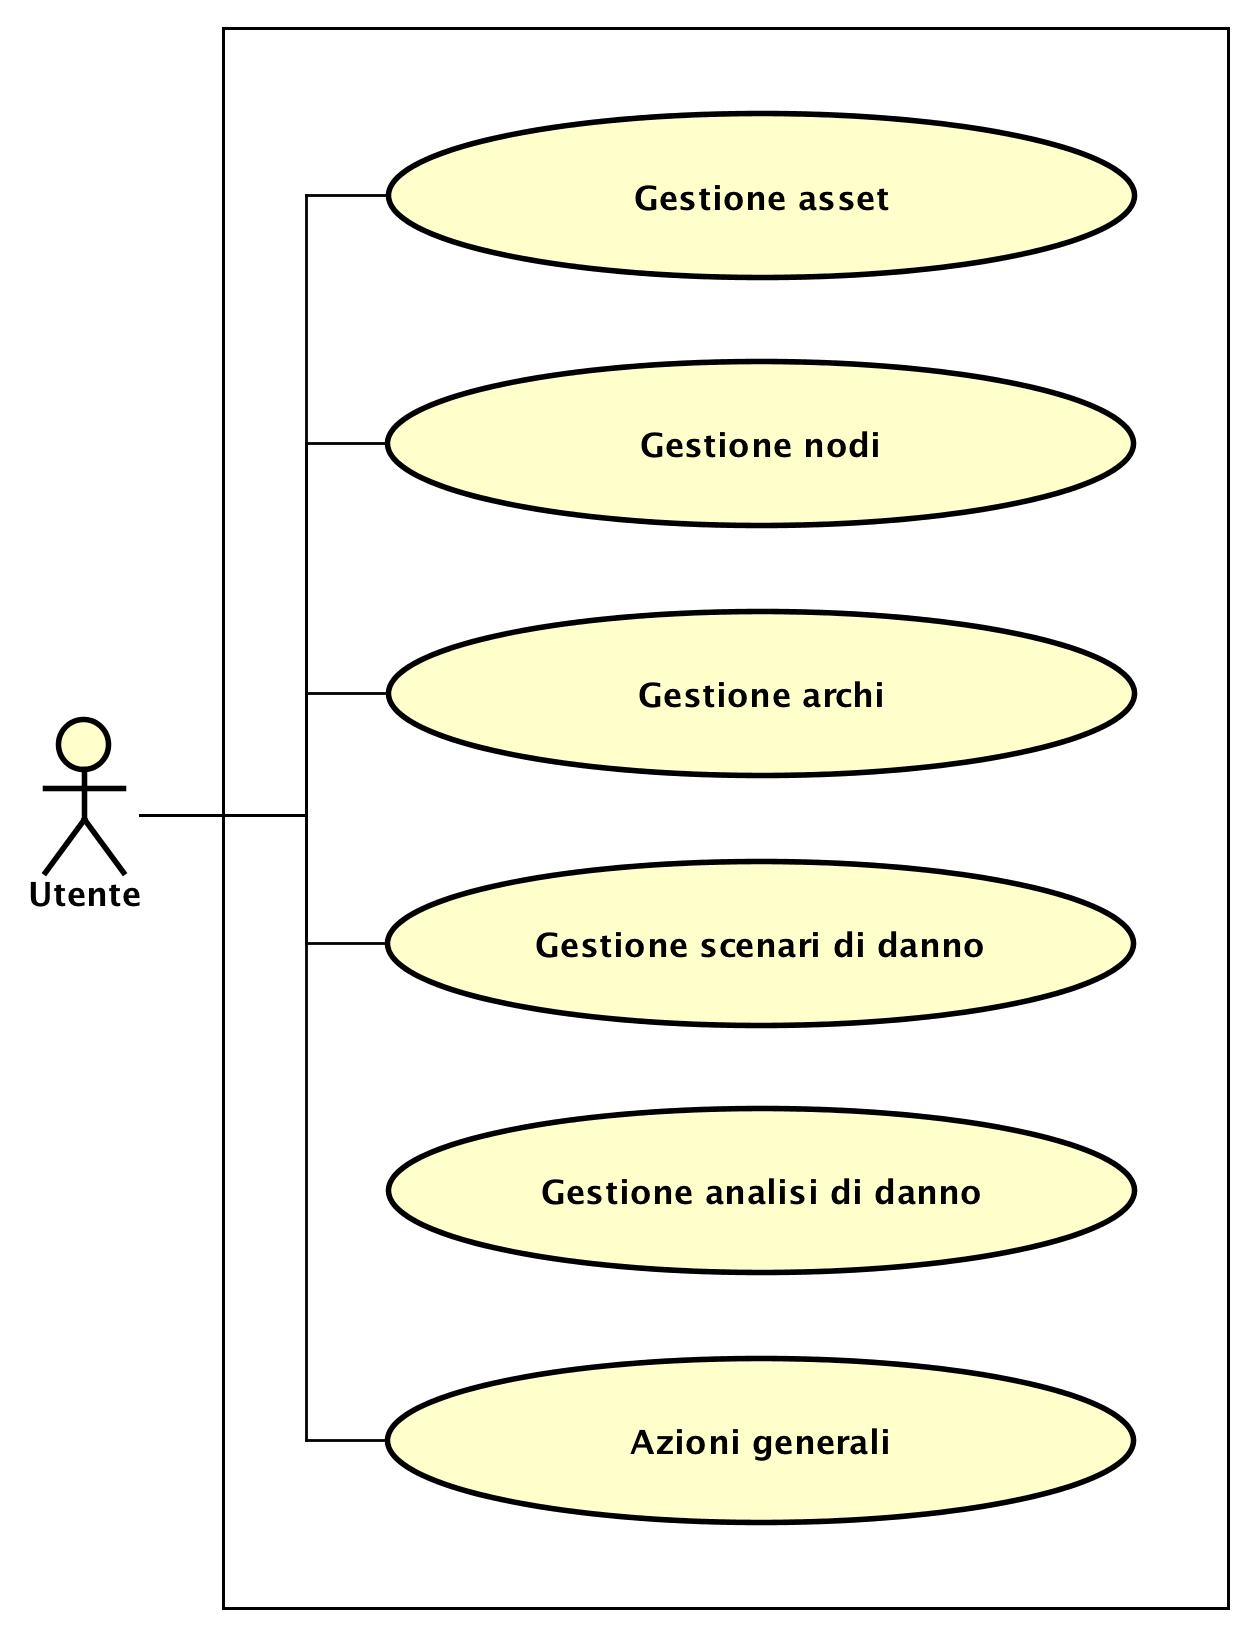
\includegraphics[width=\textwidth]{{img/uc00}.png}
		\caption{Panoramica dei casi d'uso - Generale}
	\end{figure}
	\begin{figure}[H]
		\centering
		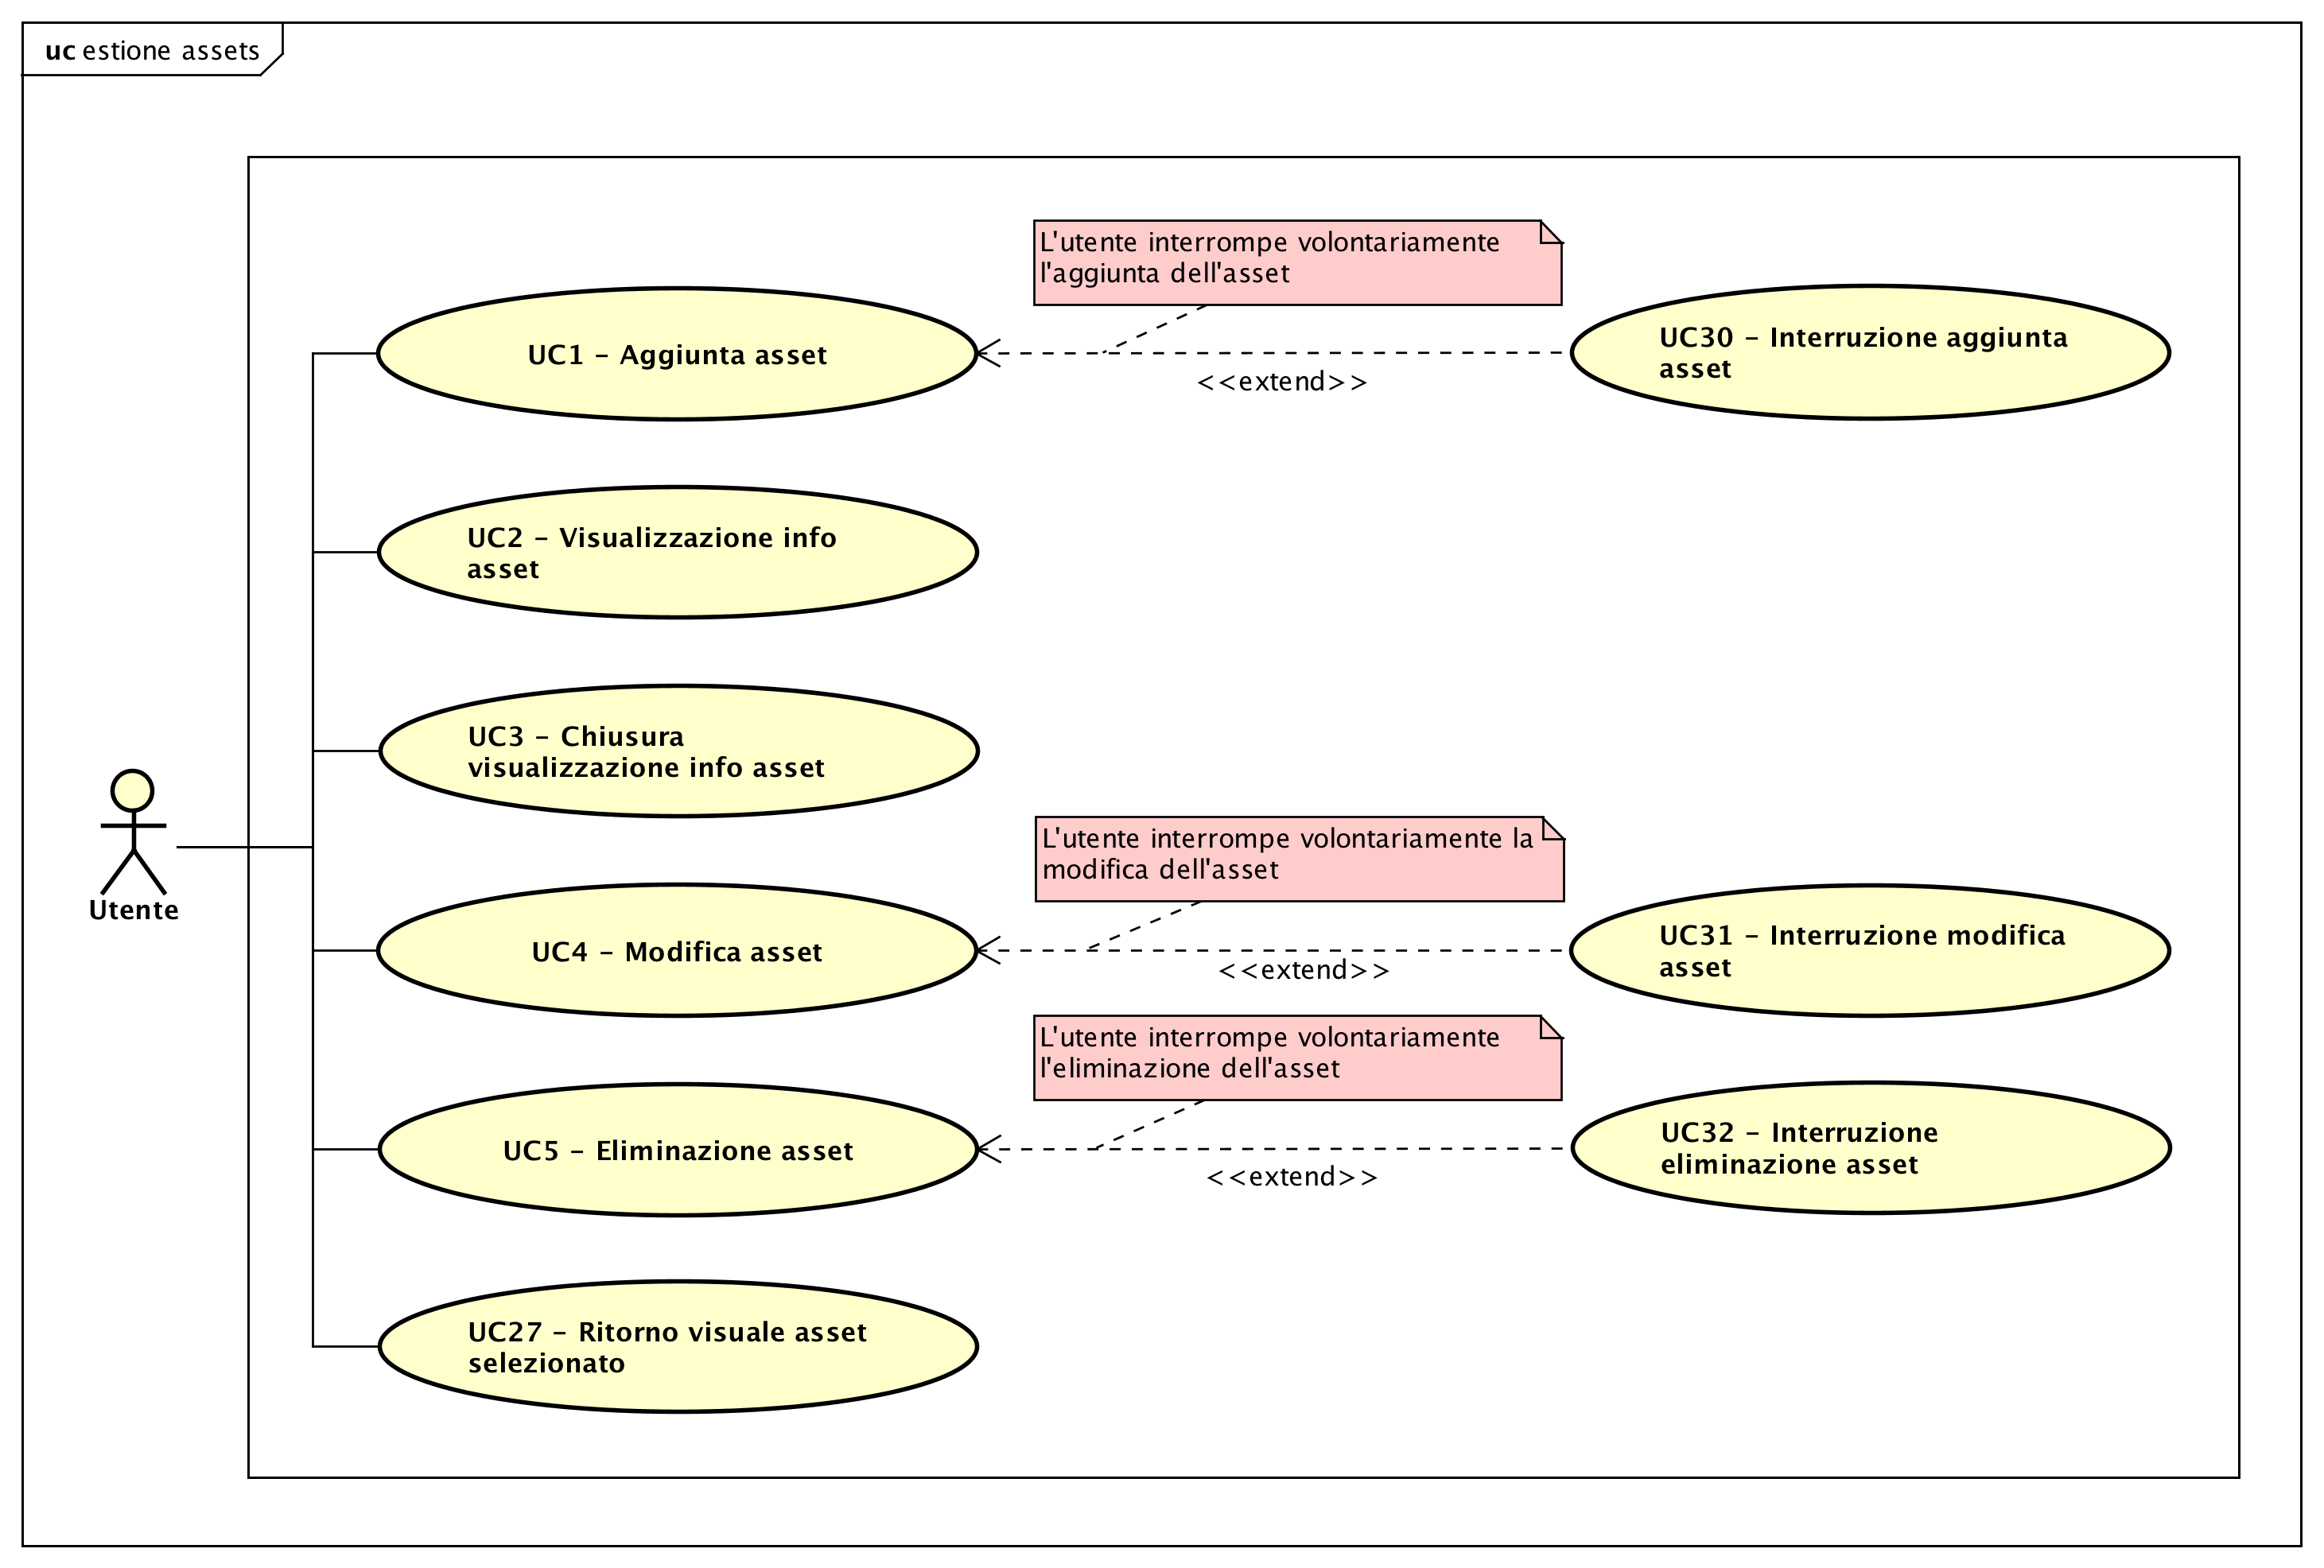
\includegraphics[width=\textwidth]{{img/uc0.1}.png}
		\caption{Panoramica dei casi d'uso - Gestione asset}
	\end{figure}
	\begin{figure}[H]
		\centering
		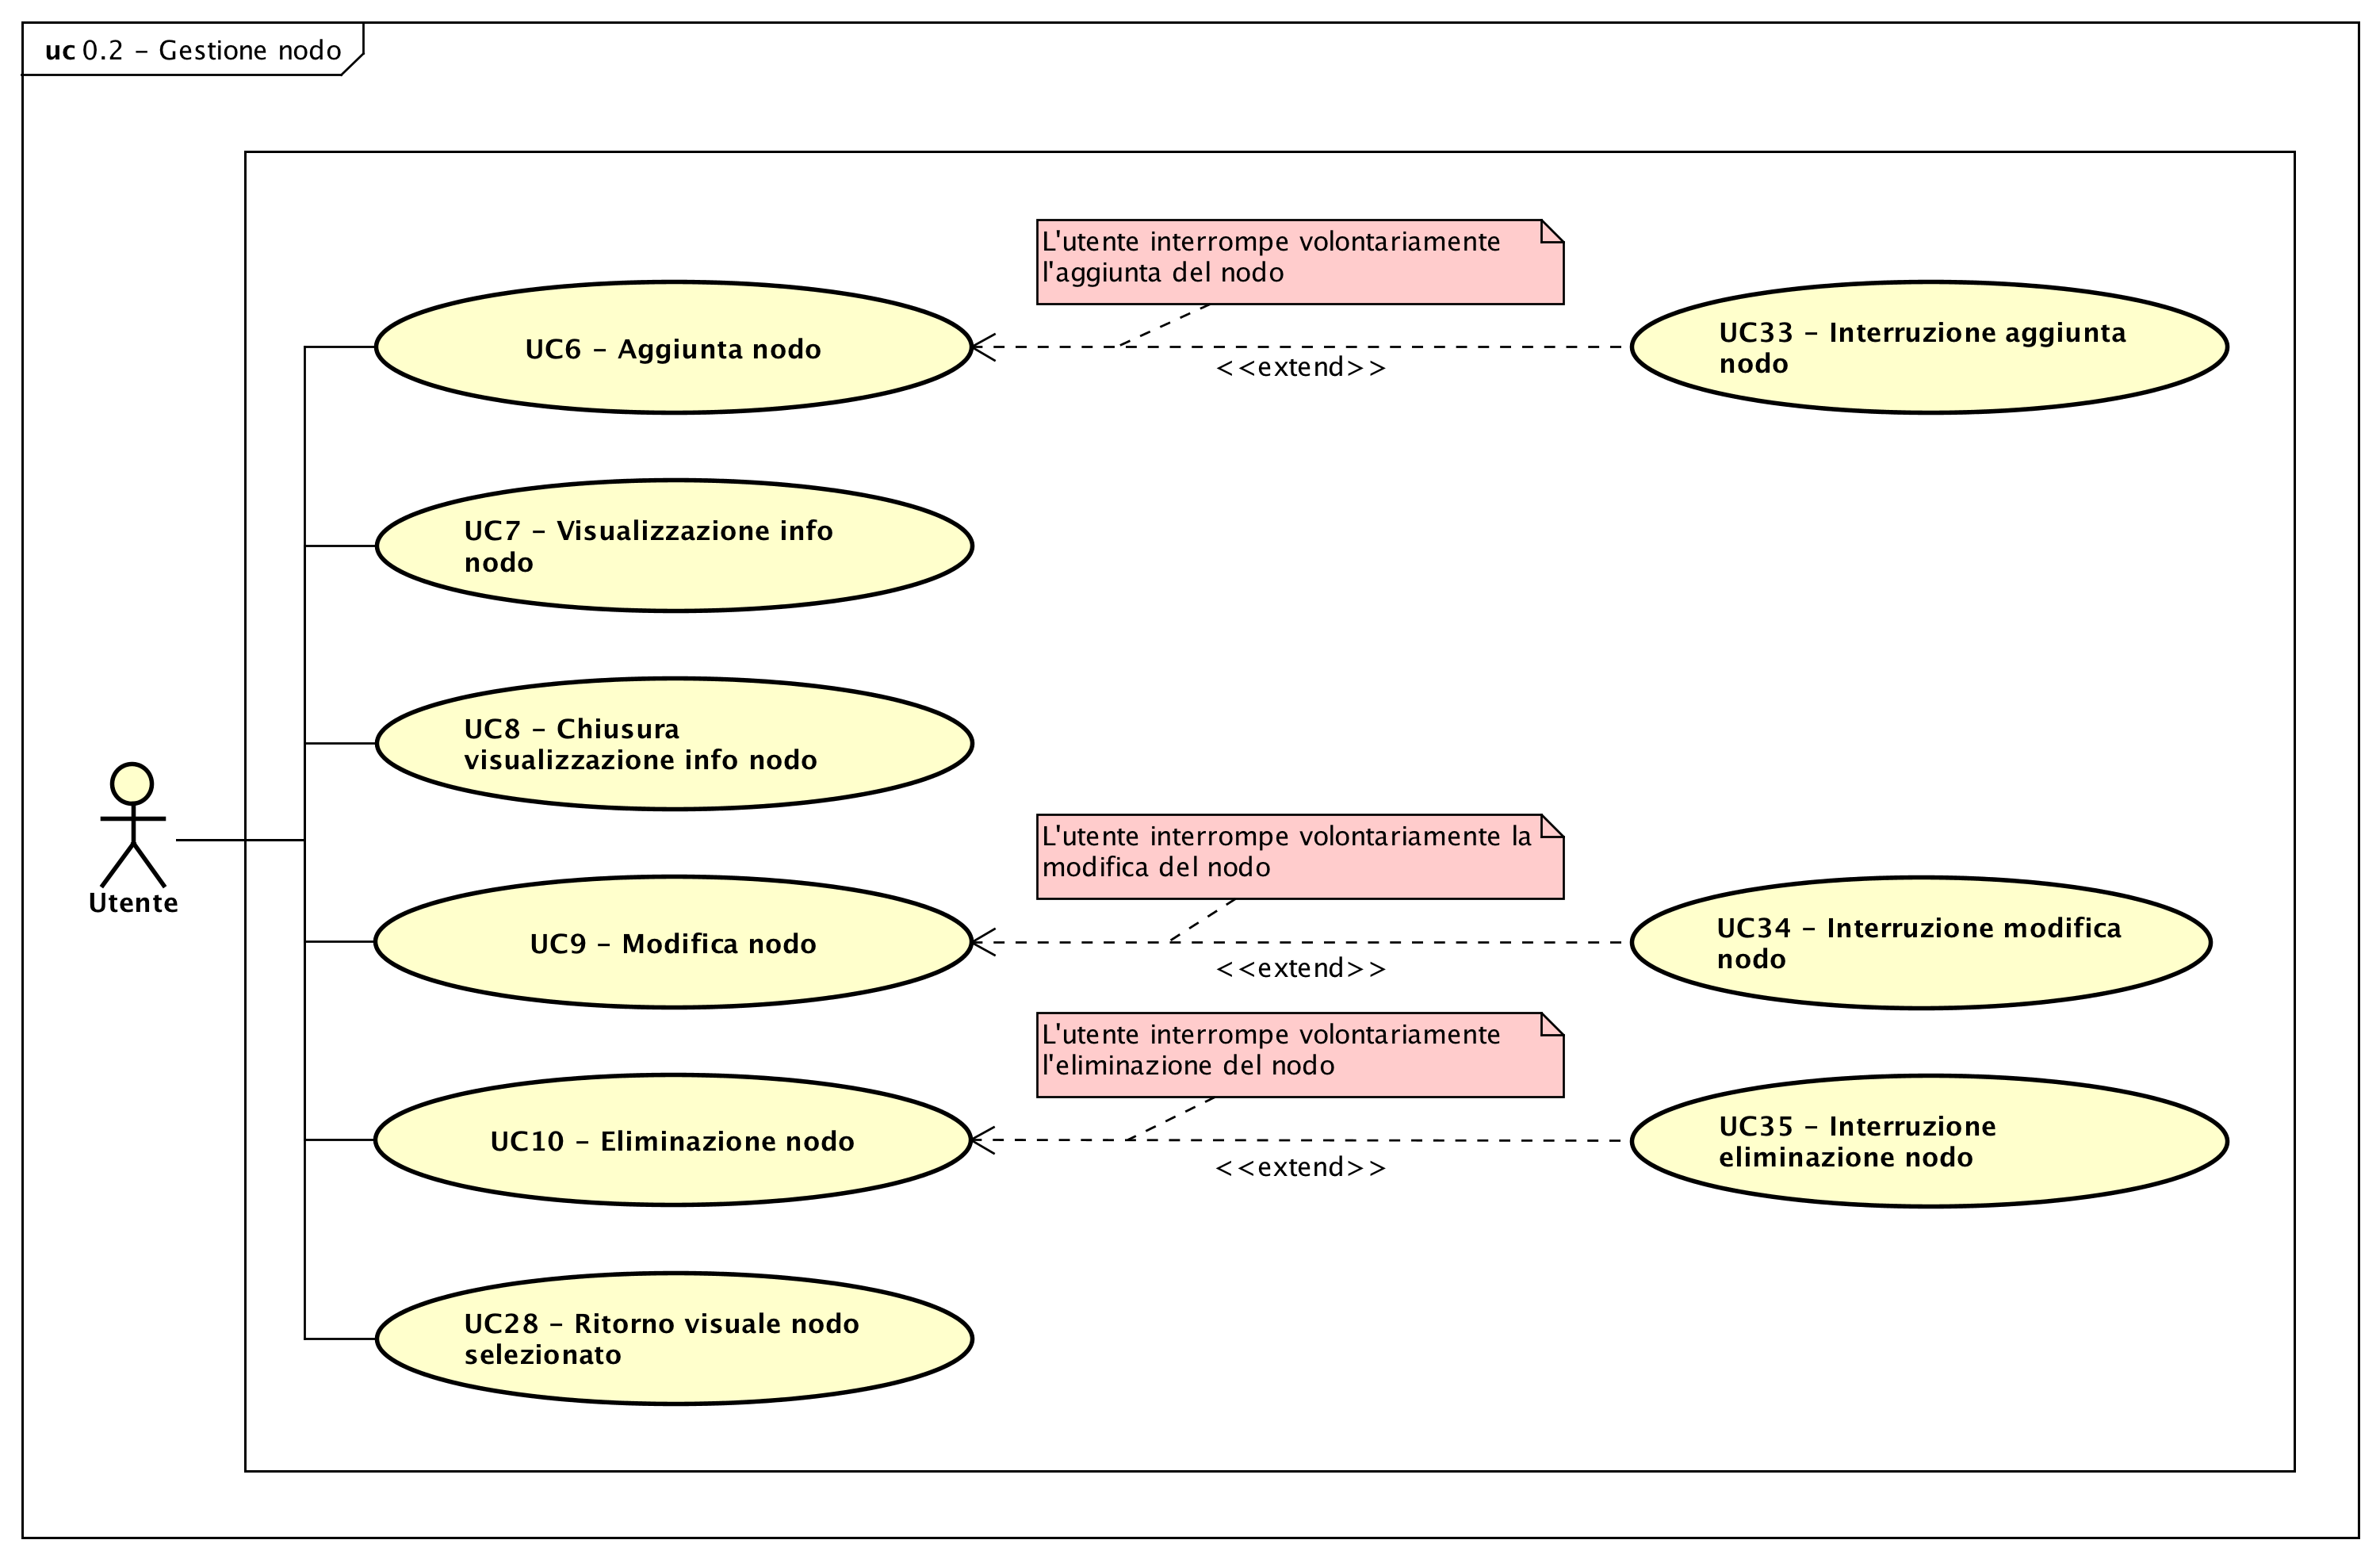
\includegraphics[width=\textwidth]{{img/uc0.2}.png}
		\caption{Panoramica dei casi d'uso - Gestione nodi}
	\end{figure}
	\begin{figure}[H]
		\centering
		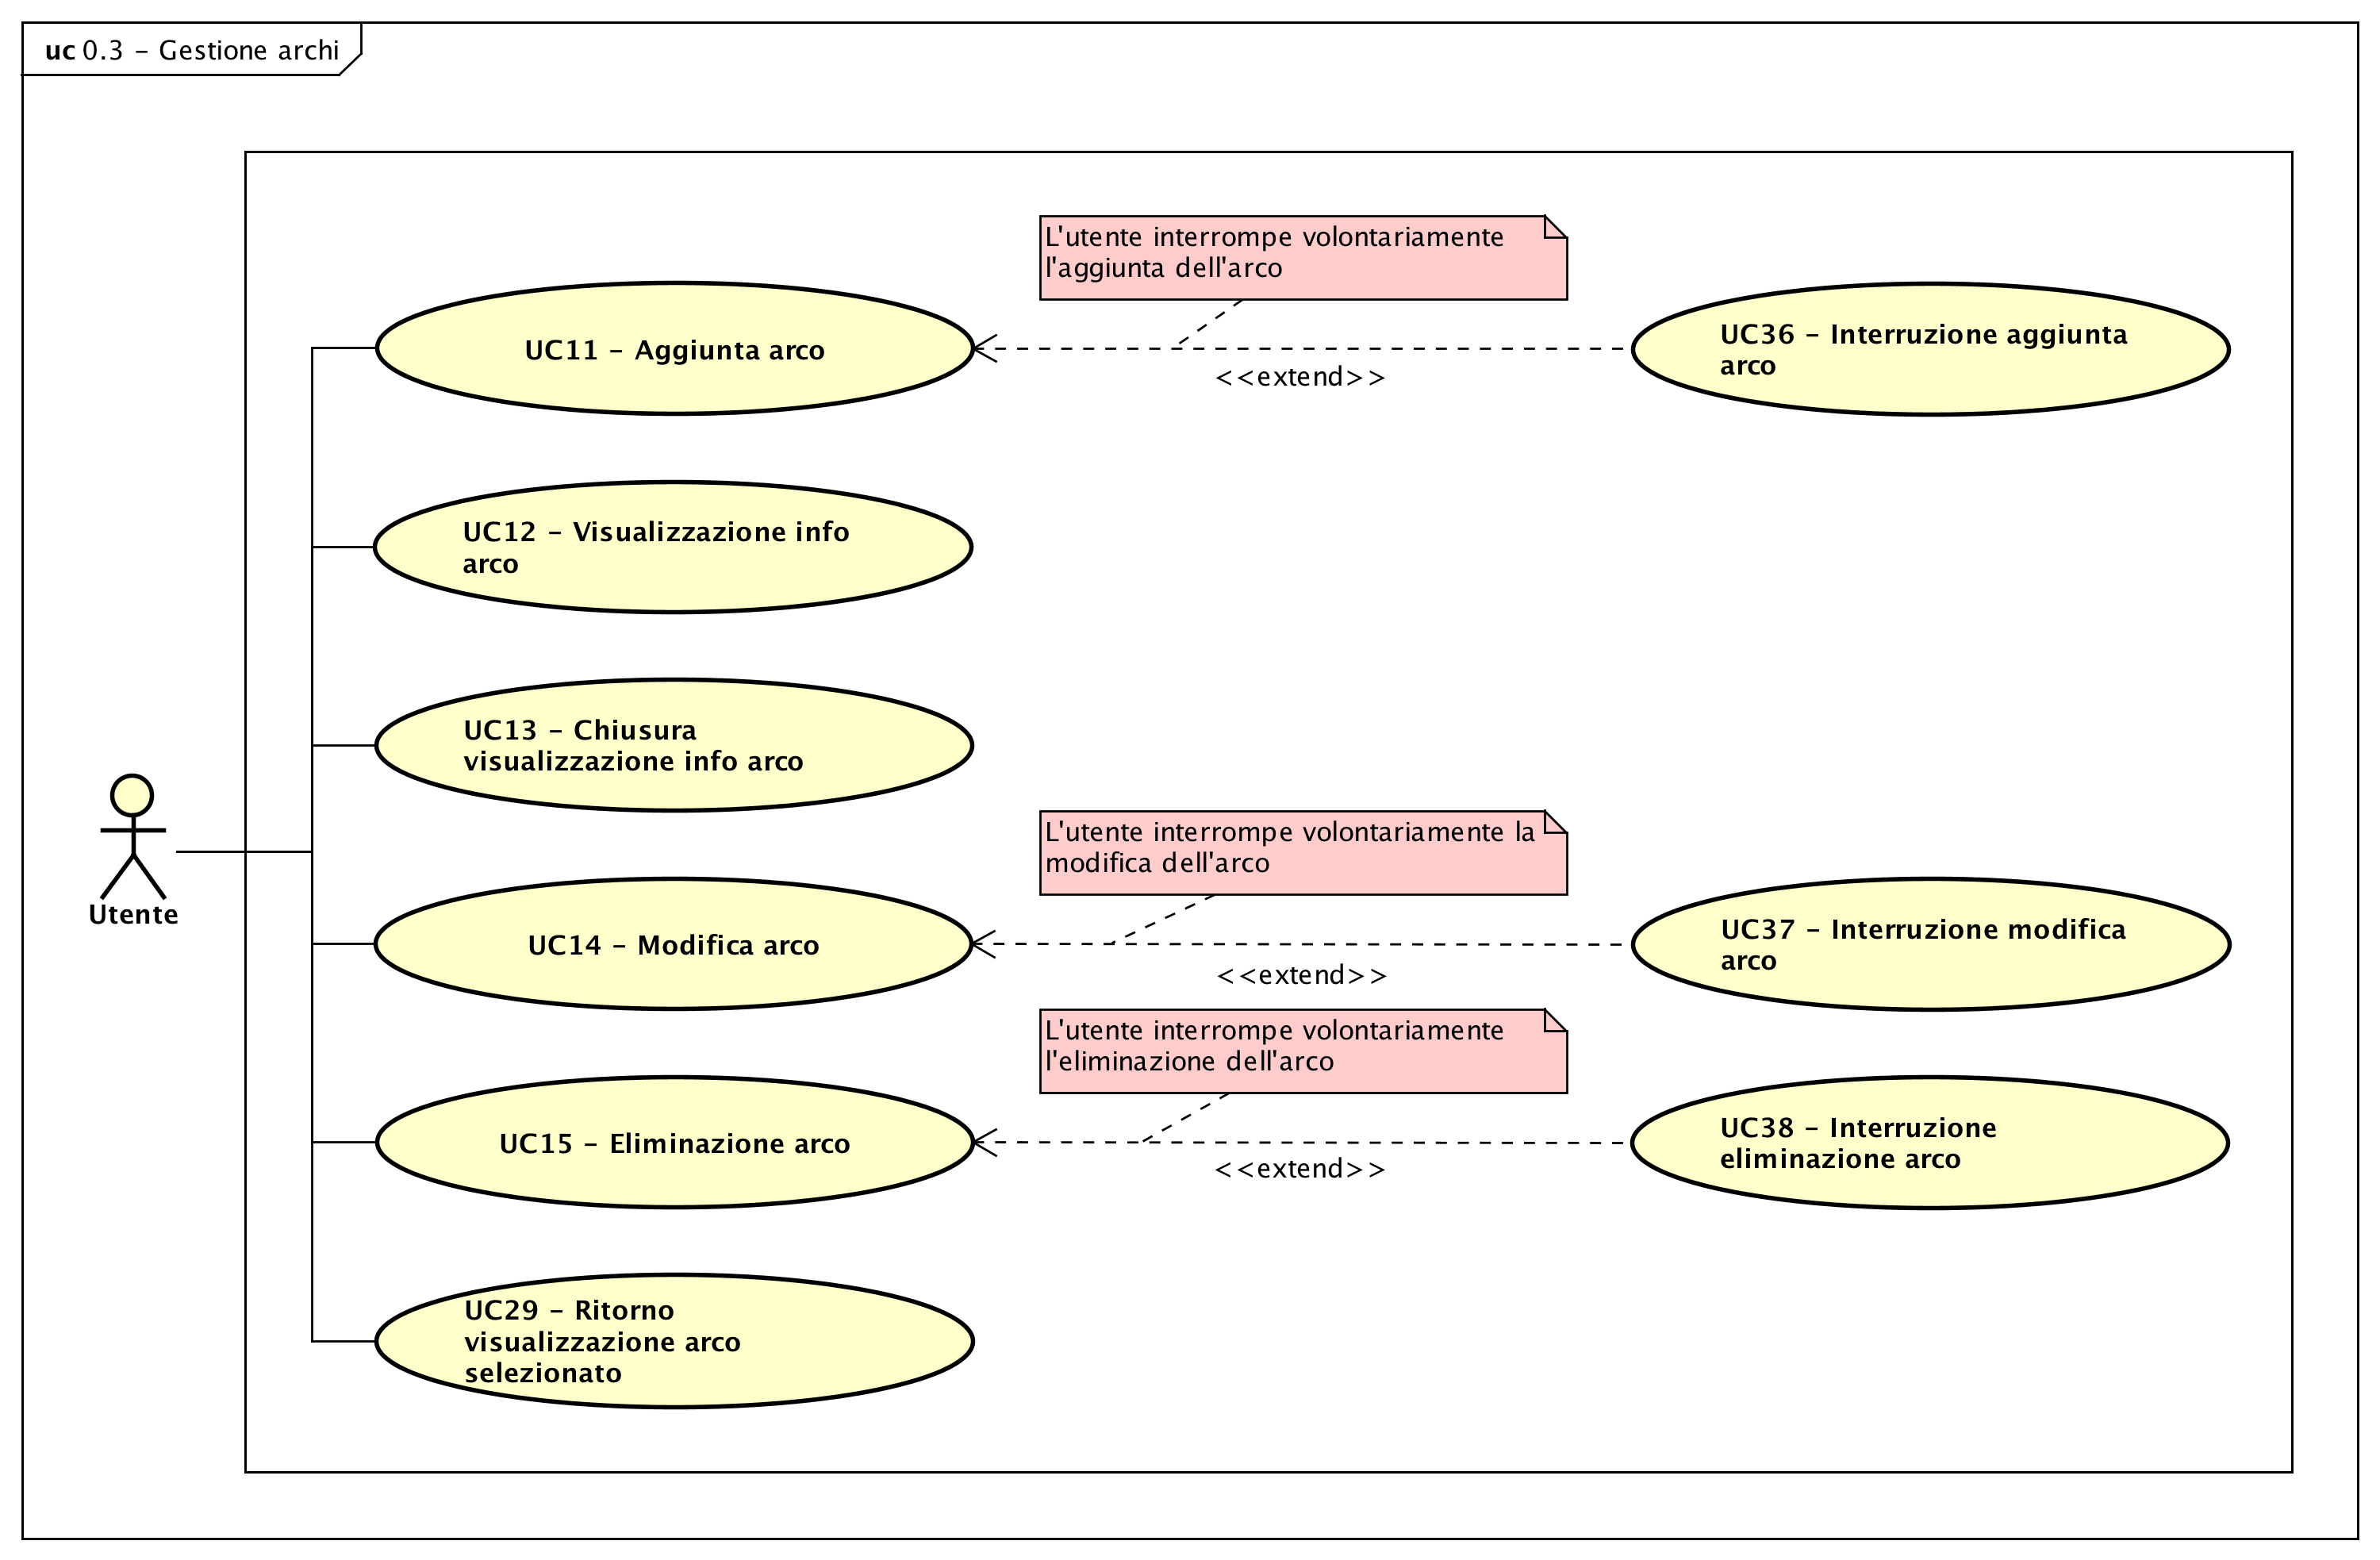
\includegraphics[width=\textwidth]{{img/uc0.3}.png}
		\caption{Panoramica dei casi d'uso - Gestione archi}
	\end{figure}
	\begin{figure}[H]
		\centering
		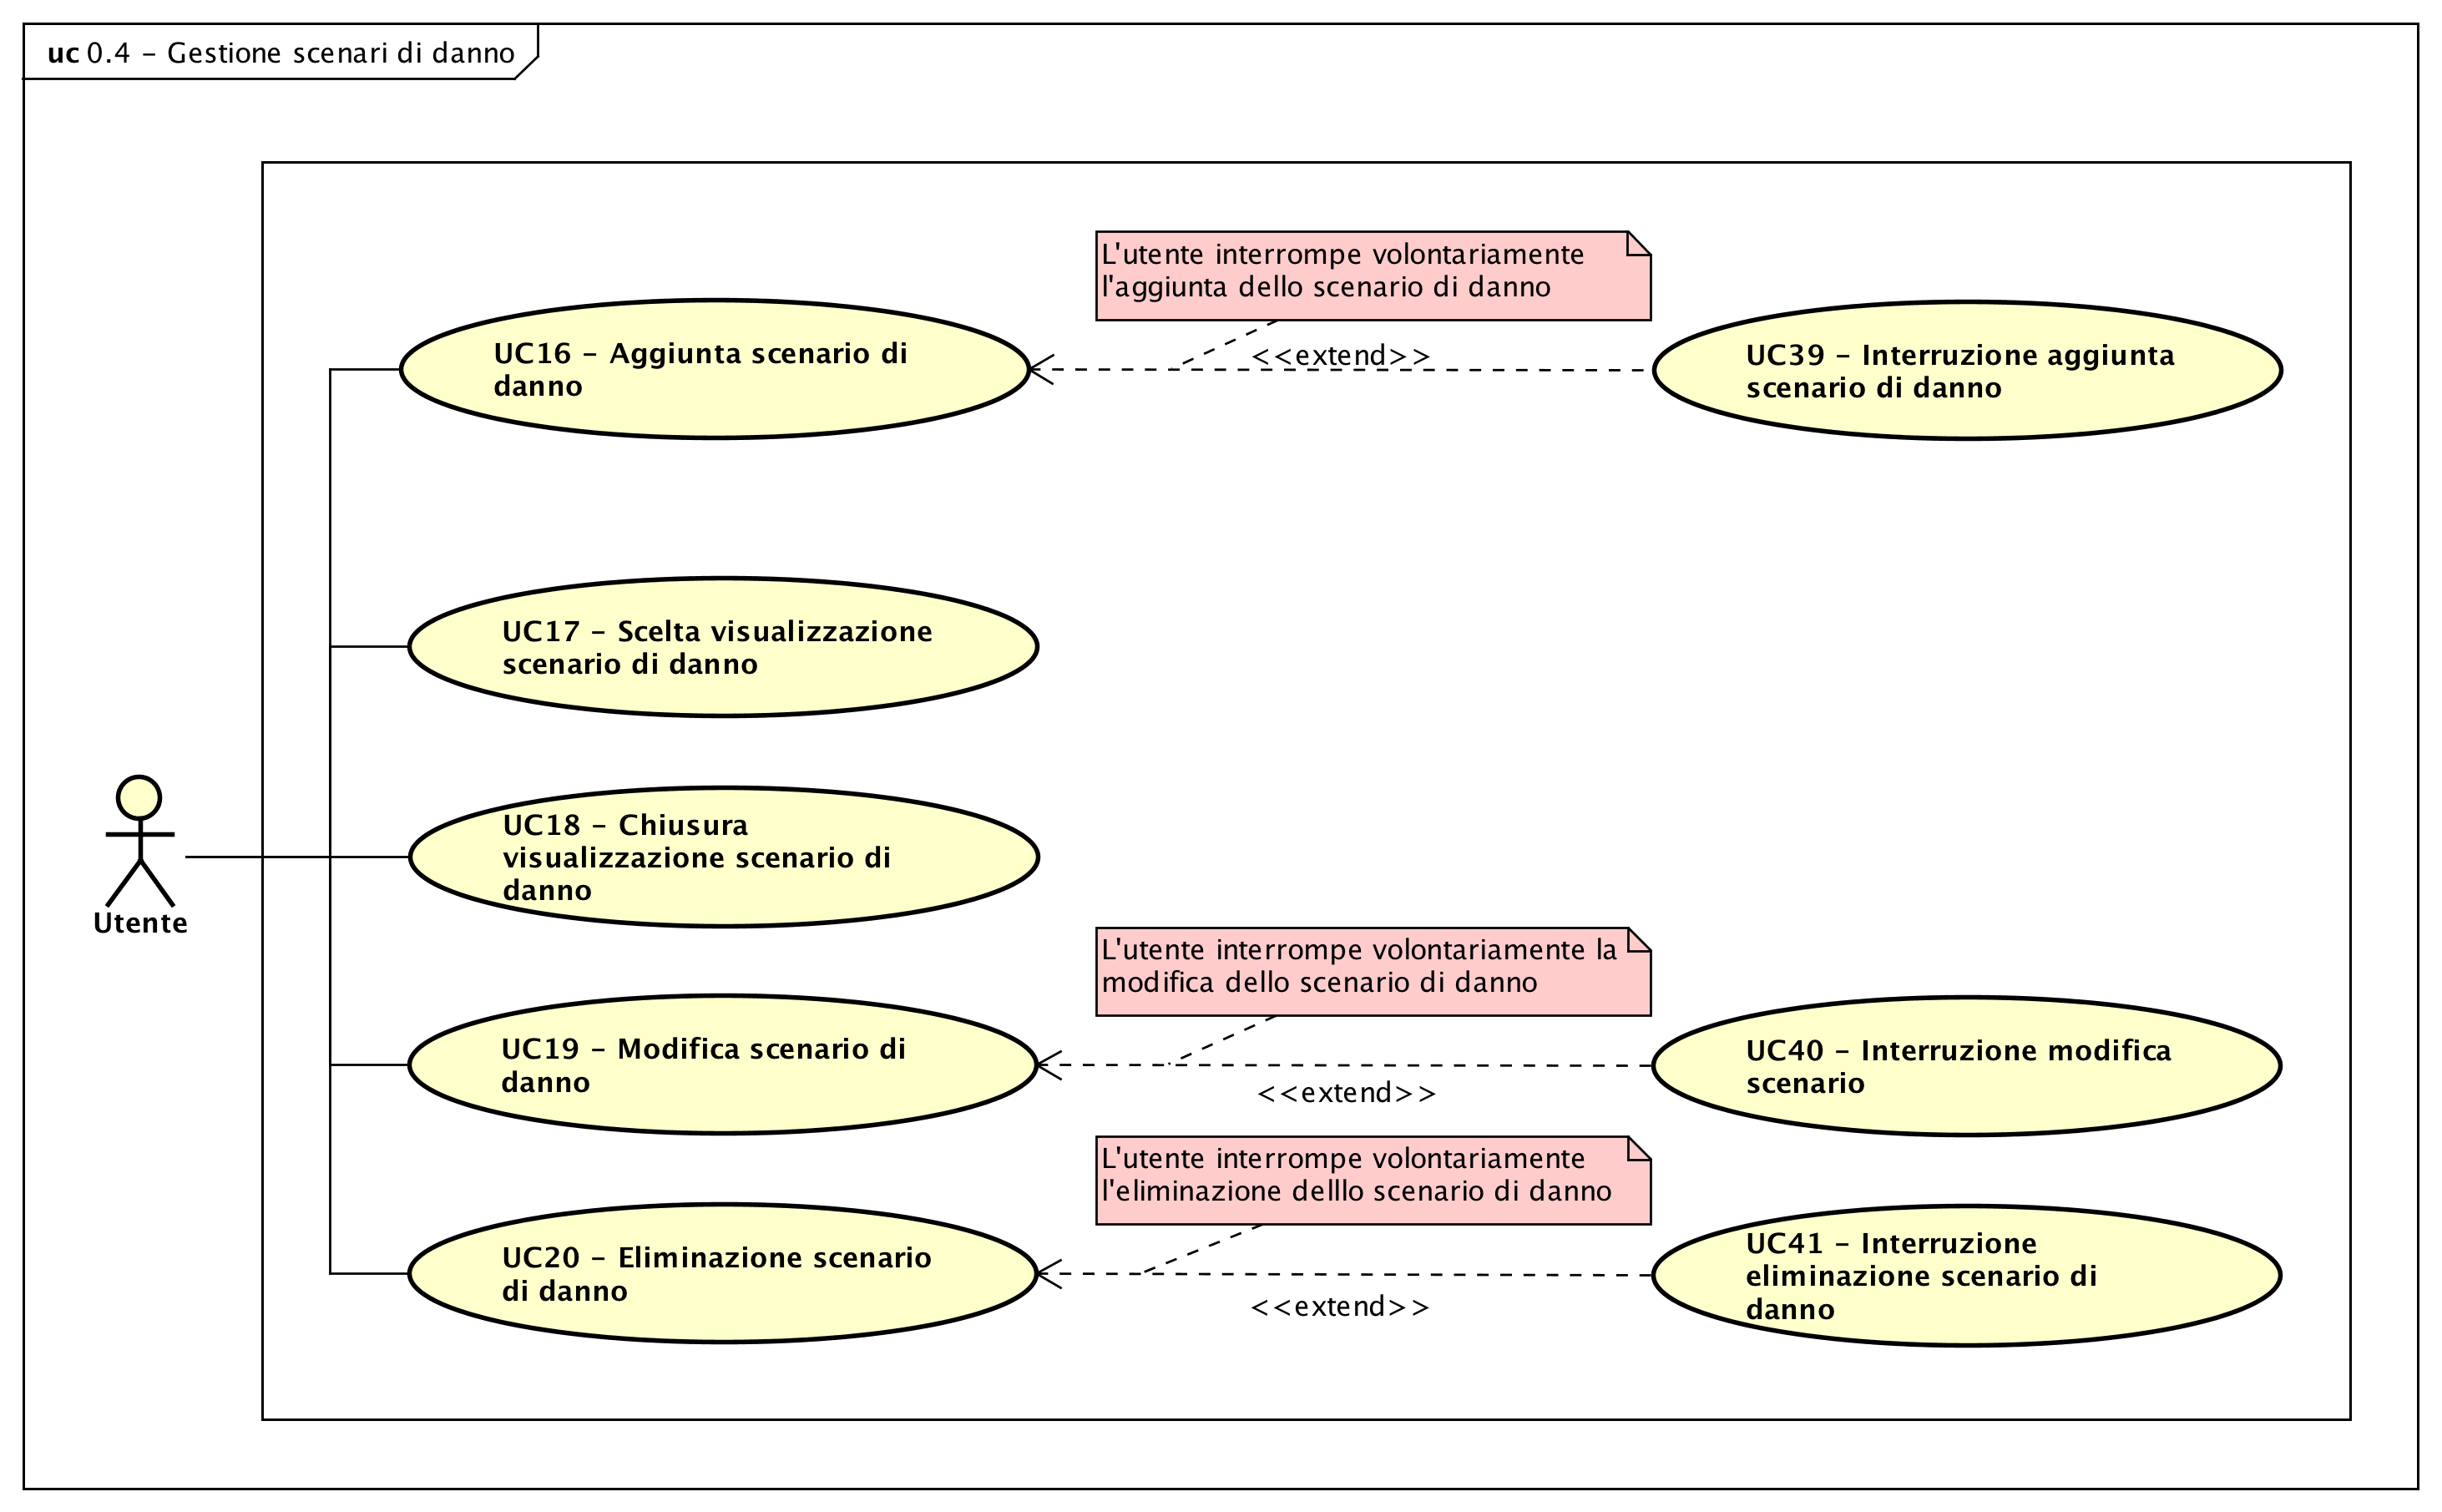
\includegraphics[width=\textwidth]{{img/uc0.4}.png}
		\caption{Panoramica dei casi d'uso - Gestione scenari di danno}
	\end{figure}
	\begin{figure}[H]
		\centering
		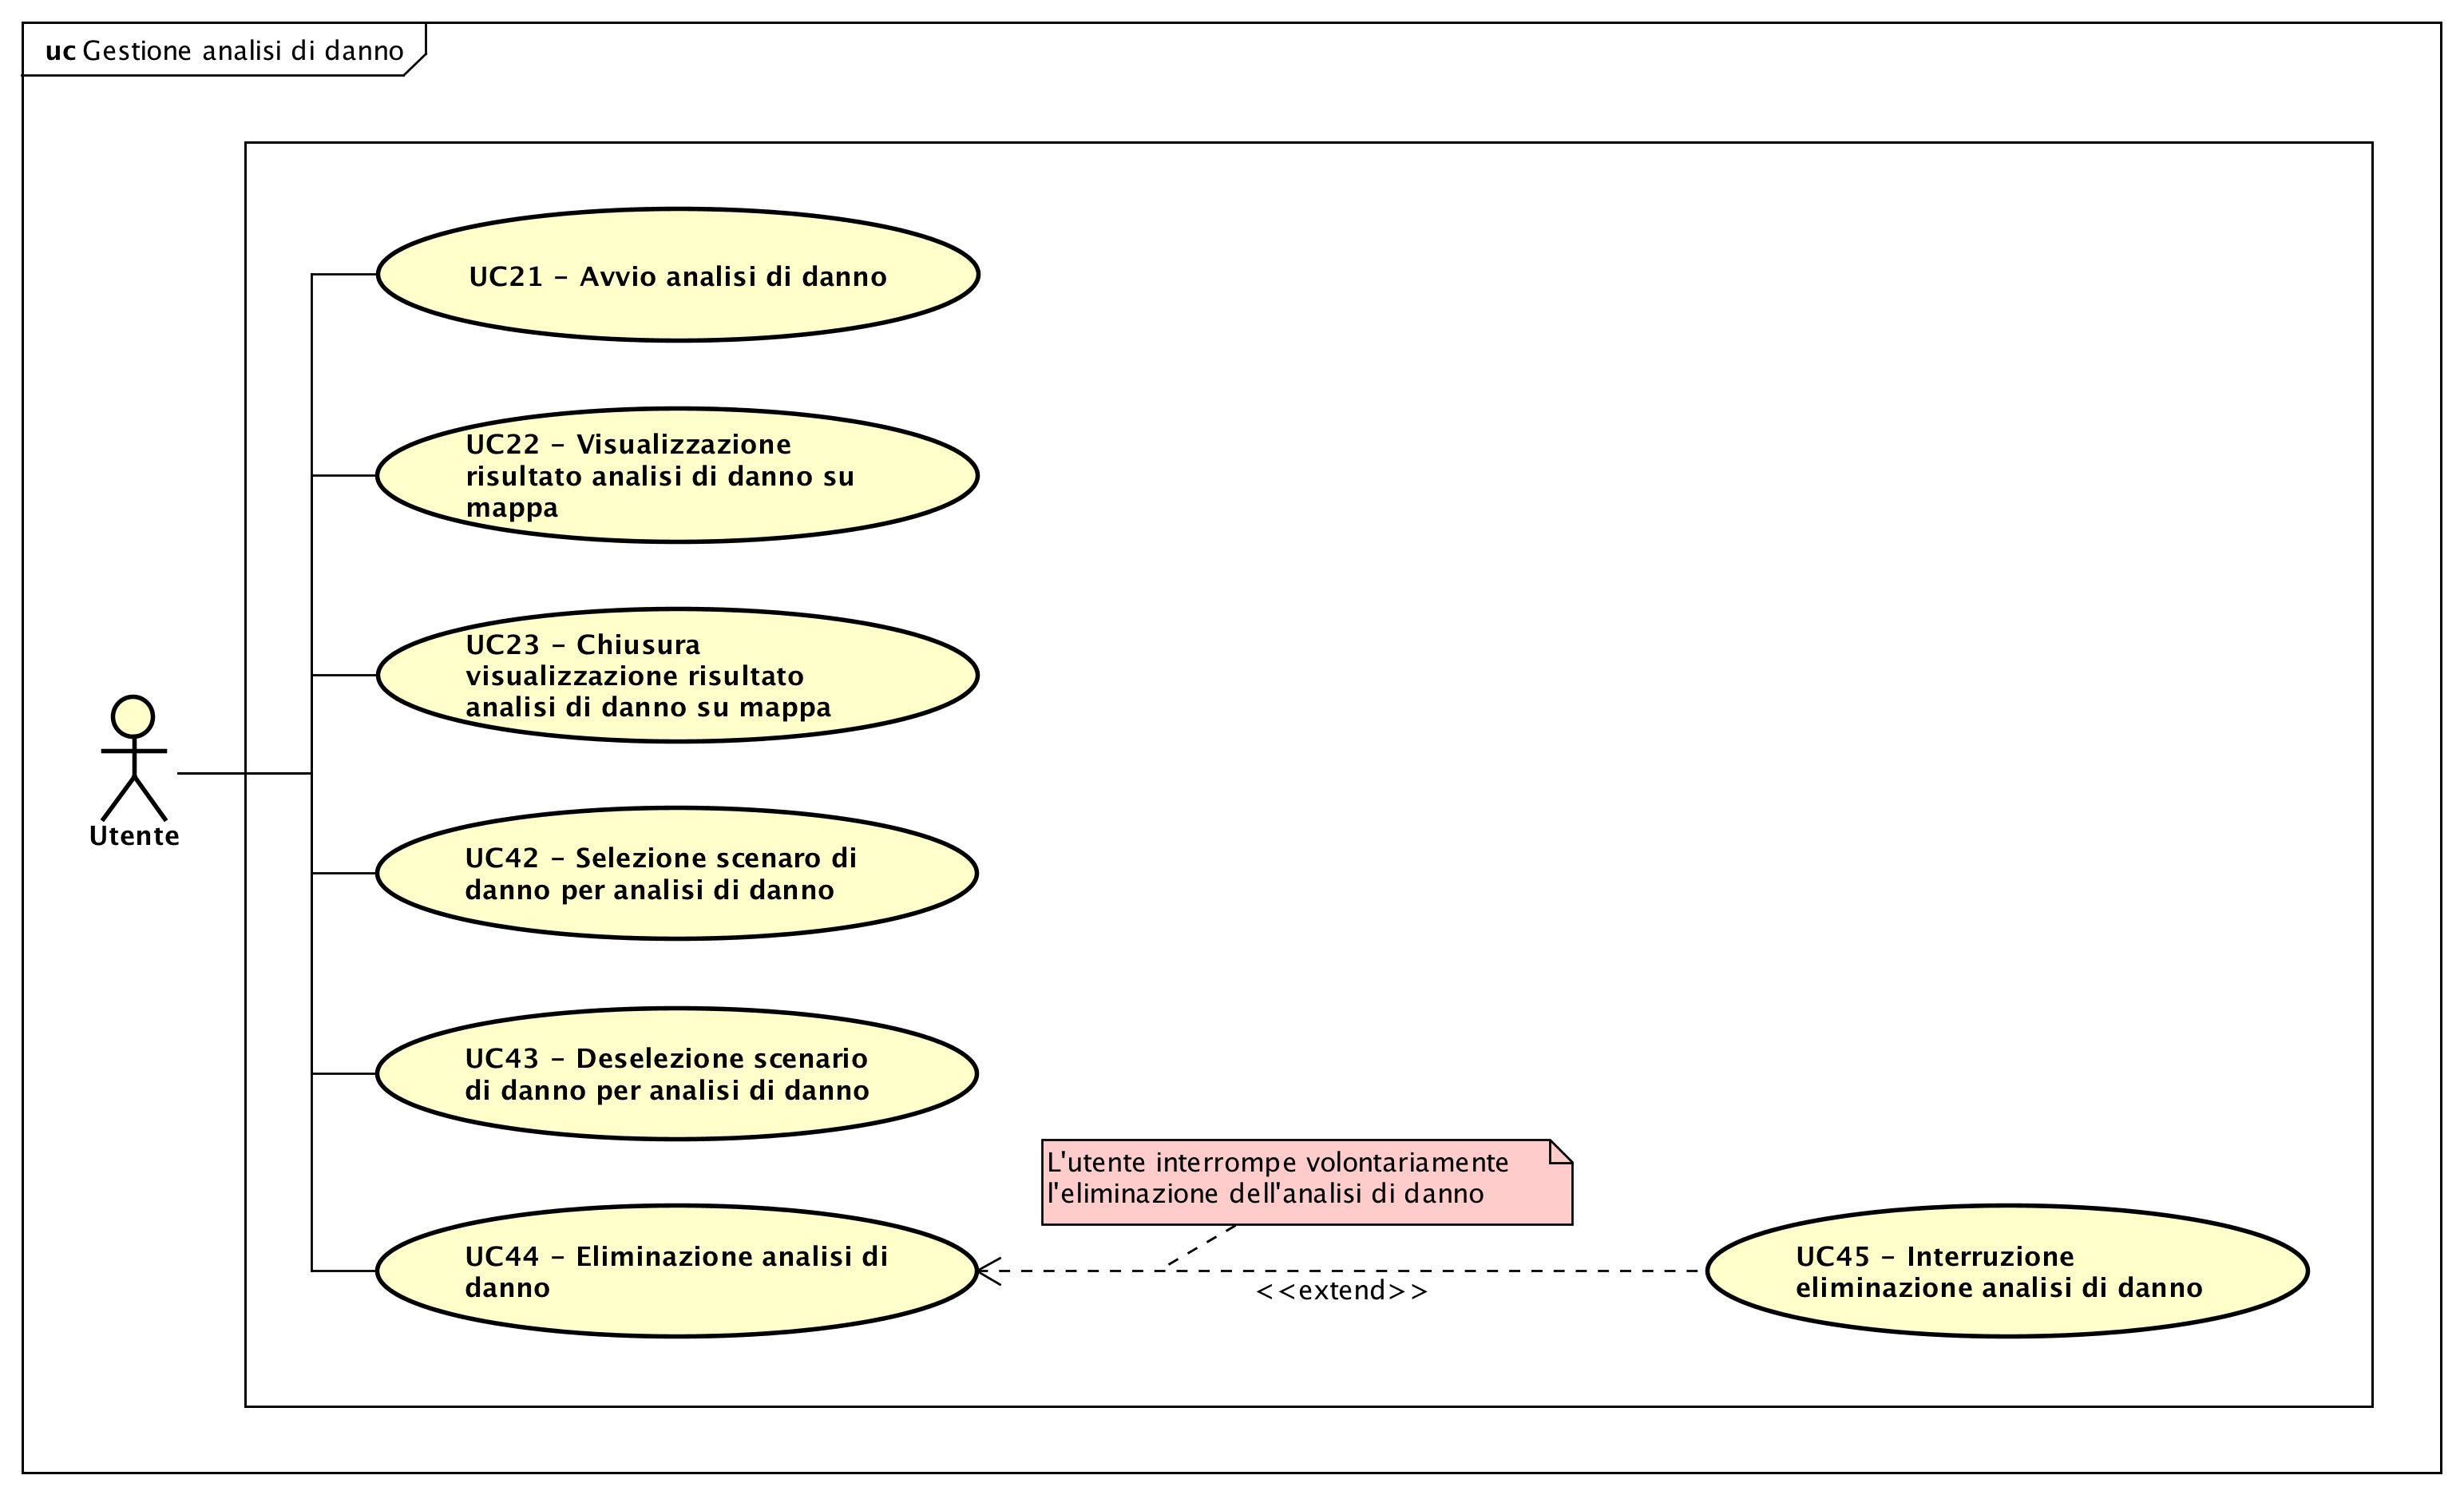
\includegraphics[width=\textwidth]{{img/uc0.5}.png}
		\caption{Panoramica dei casi d'uso - Gestione analisi di danno}
	\end{figure}
	\begin{figure}[H]
		\centering
		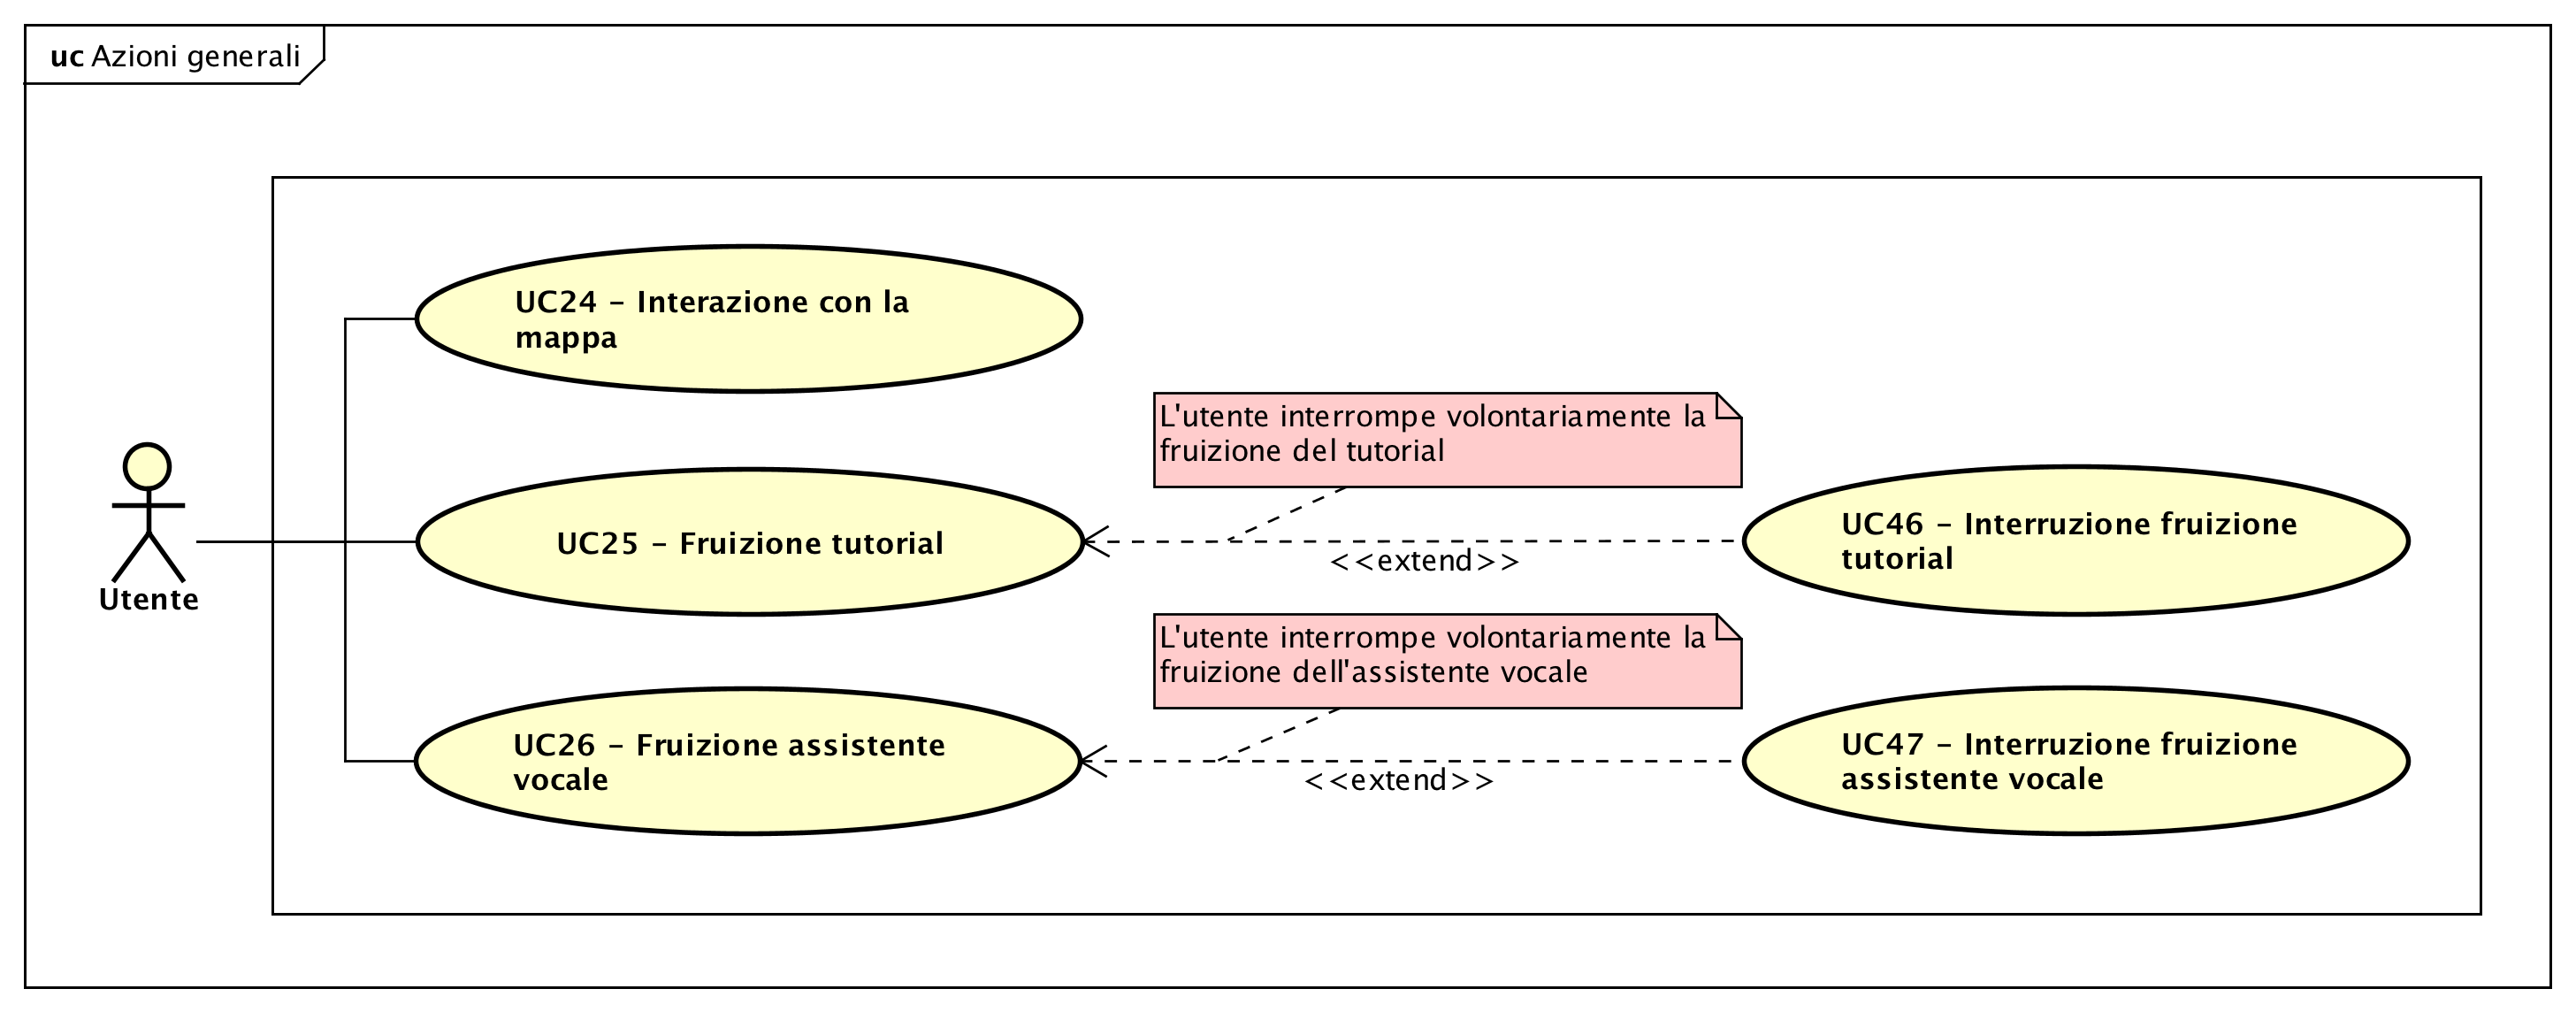
\includegraphics[width=\textwidth]{{img/uc0.6}.png}
		\caption{Panoramica dei casi d'uso - Azioni generali}
	\end{figure}
\subsection{UC1 - Aggiunta asset} 
\label{sssec:UC1} 
\begin{figure}[H] 
	\centering 
	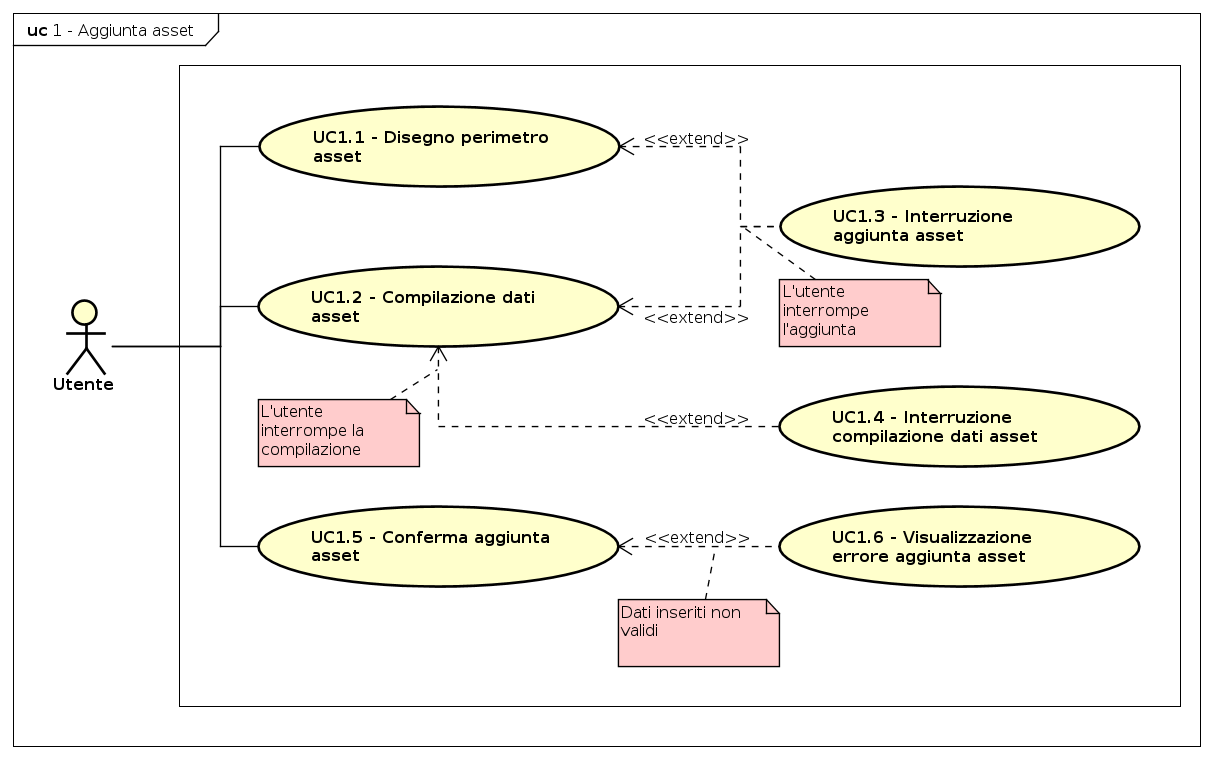
\includegraphics[width=\textwidth]{{img/uc1}.png} 
	\caption{UC1 - Aggiunta asset}
\end{figure}
\def\arraystretch{1.5}
\rowcolors{2}{D}{P}
\begin{tabularx}{\textwidth}{l|p{0.7\textwidth}}
	\rowcolor{I} \multicolumn{2}{c}{\color{white}\textbf{UC1 - Aggiunta asset}} \\
	\toprule
	\endhead
	\textbf{Attori} & Utente\\
	\textbf{Descrizione} & l'utente aggiunge un asset\\
	\textbf{Pre-condizione} & l'utente ha aperto l'applicazione\\
	\textbf{Post-condizione} & un nuovo asset è stato aggiunto ed è visualizzabile sulla mappa; l'utente visualizza un messaggio che comunica la corretta esecuzione dell'operazione; l'area informativa rimane impostata sull'asset appena inserito; la posizione e il livello di ingrandimento della mappa rimangono invariati\\
	\textbf{Scenario principale} & \vspace{-1.2em}\begin{enumerate}[leftmargin=*,noitemsep,nosep]
		\item \nameref{sssec:UC1.1};
		\item \nameref{sssec:UC1.2};
		\item \nameref{sssec:UC1.4}.
	\end{enumerate}\\
	\textbf{Estensioni} & \vspace{-1.2em}\begin{itemize}[leftmargin=*,noitemsep,nosep]
		\item \nameref{sssec:UC30}: l’utente interrompe volontariamente l’aggiunta dell’asset
	\end{itemize}\\
	\textbf{Scenari alternativi} & \vspace{-1.2em}\begin{itemize}[leftmargin=*,noitemsep,nosep]
		\item \nameref{sssec:UC1.3};
		\item \nameref{sssec:UC1.5}.
	\end{itemize}\\
	%\textbf{Generalizzazioni} &  \\
	\bottomrule
\end{tabularx}
\subsection{UC1.1 - Disegno perimetro asset} 
\label{sssec:UC1.1} 
\begin{figure}[H] 
	\centering 
	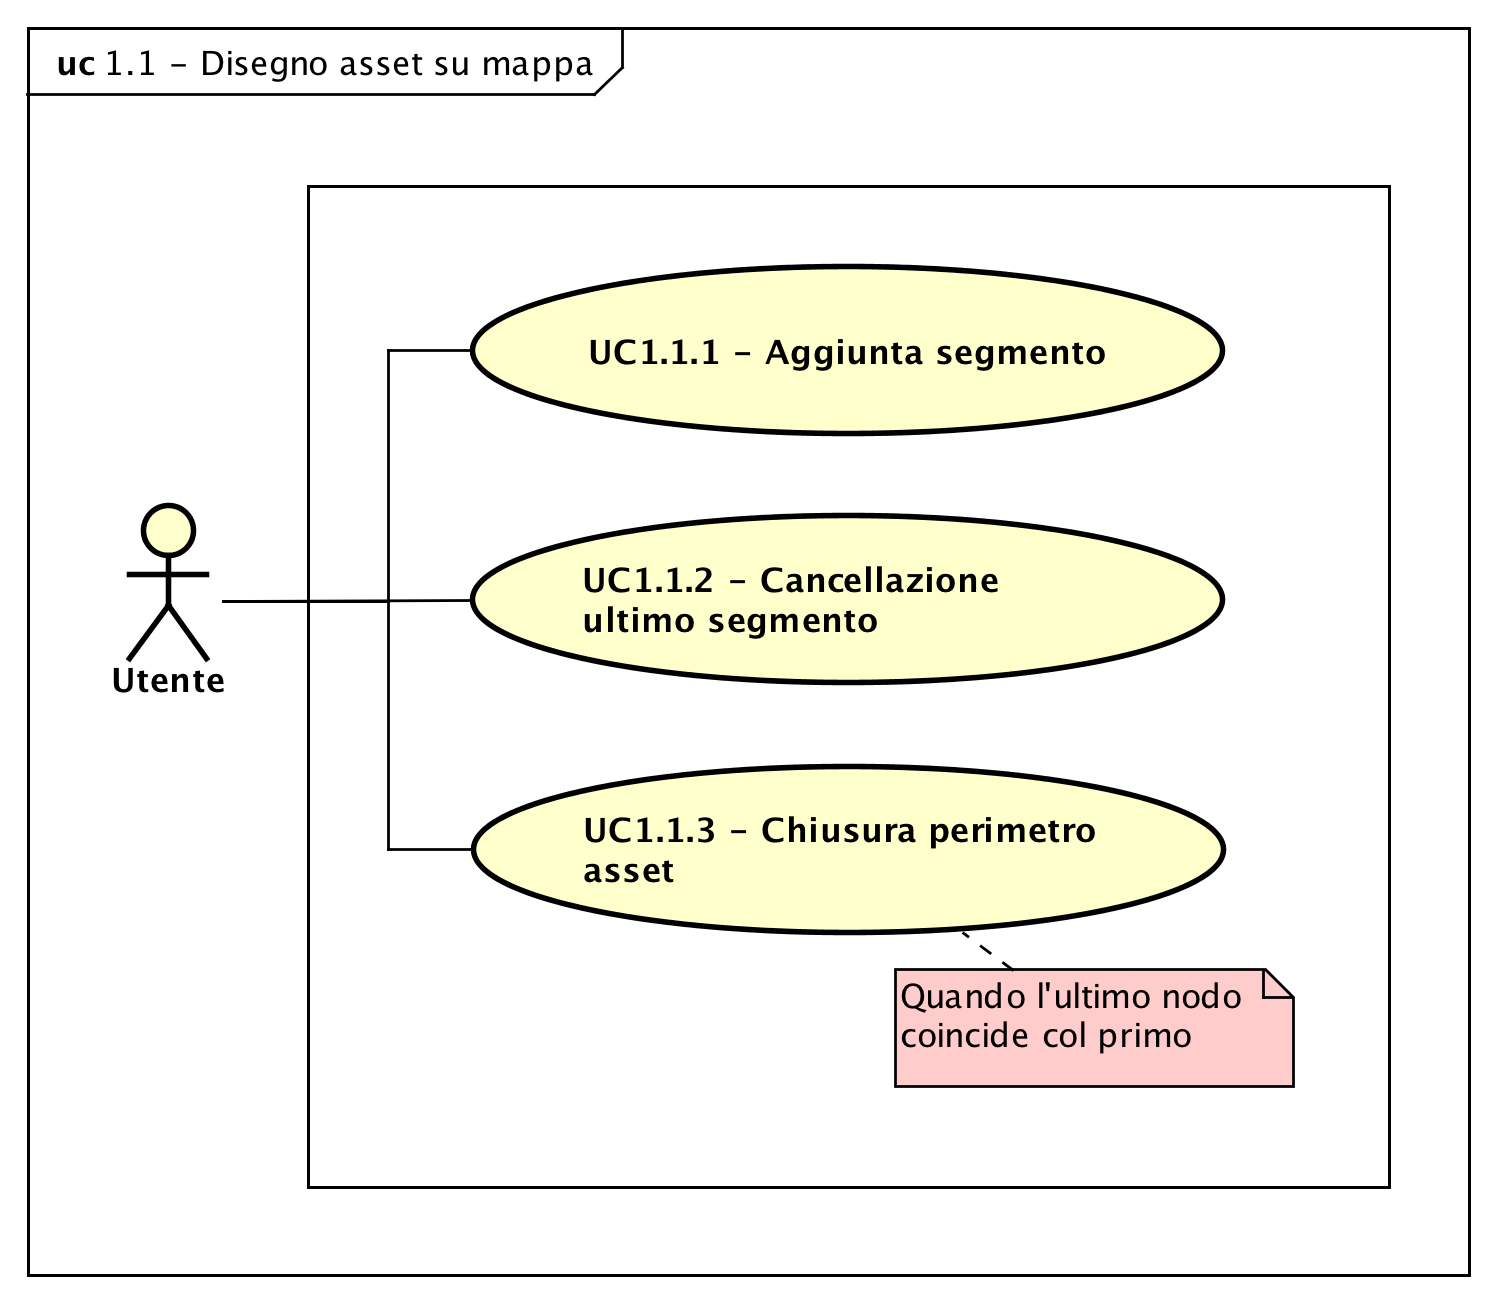
\includegraphics[scale=0.5]{{img/uc1.1}.png} 
	\caption{UC1.1 - Disegno perimetro asset}
\end{figure}
\def\arraystretch{1.5}
\rowcolors{2}{D}{P}
\begin{tabularx}{\textwidth}{l|p{0.7\textwidth}}
	\rowcolor{I} \multicolumn{2}{c}{\color{white}\textbf{UC1.1 - Disegno perimetro asset}} \\
	\toprule
	\endhead
	\textbf{Attori} & Utente\\
	\textbf{Descrizione} & l'utente disegna su mappa il perimetro dell'asset\\
	\textbf{Pre-condizione} & il sistema offre la possibilità di disegnare su mappa il perimetro dell'asset\\
	\textbf{Post-condizione} & il perimetro dell'asset è stato disegnato e viene visualizzato sulla mappa; l'utente può procedere alla compilazione dei restanti dati dell'asset nell'area informativa\\
	\textbf{Scenario principale} & \vspace{-1.2em}\begin{enumerate}[leftmargin=*,noitemsep,nosep]
		\item \nameref{sssec:UC1.1.1};
		\item \nameref{sssec:UC1.1.2};
		\item \nameref{sssec:UC1.1.3}.
	\end{enumerate}\\
	%\textbf{Generalizzazioni} &  \\
	\bottomrule
\end{tabularx}
\subsection{UC1.1.1 - Aggiunta segmento} 
\label{sssec:UC1.1.1} 
\def\arraystretch{1.5}
\rowcolors{2}{D}{P}
\begin{tabularx}{\textwidth}{l|p{0.7\textwidth}}
	\rowcolor{I} \multicolumn{2}{c}{\color{white}\textbf{UC1.1.1 - Aggiunta segmento}} \\
	\toprule
	\endhead
	\textbf{Attori} & Utente\\
	\textbf{Descrizione} & l'utente aggiunge un segmento al perimetro dell'asset che sta disegnando\\
	\textbf{Pre-condizione} & il sistema offre la possibilità di aggiungere un segmento al perimetro dell'asset\\
	\textbf{Post-condizione} & l'utente ha aggiunto un segmento al perimetro dell'asset che sta disegnando; il segmento viene visualizzato sulla mappa\\
	\textbf{Scenario principale} & \vspace{-1.2em}\begin{enumerate}[leftmargin=*,noitemsep,nosep]
		\item \nameref{sssec:UC1.1.1}.
	\end{enumerate}\\
	%\textbf{Generalizzazioni} &  \\
	\bottomrule
\end{tabularx}
\subsection{UC1.1.2 - Cancellazione ultimo segmento} 
\label{sssec:UC1.1.2} 
\def\arraystretch{1.5}
\rowcolors{2}{D}{P}
\begin{tabularx}{\textwidth}{l|p{0.7\textwidth}}
	\rowcolor{I} \multicolumn{2}{c}{\color{white}\textbf{UC1.1.2 - Cancellazione ultimo segmento}} \\
	\toprule
	\endhead
	\textbf{Attori} & Utente\\
	\textbf{Descrizione} & l'utente cancella l'ultimo segmento del perimetro dell'asset che sta disegnando\\
	\textbf{Pre-condizione} & l'utente sta disegnando il perimetro di un asset; è stato disegnato almeno un segmento\\
	\textbf{Post-condizione} & l'utente ha cancellato l'ultimo segmento del perimetro dell'asset che sta disegnando; l'ultimo segmento non è più visualizzato sulla mappa\\
	\textbf{Scenario principale} & \vspace{-1.2em}\begin{enumerate}[leftmargin=*,noitemsep,nosep]
		\item \nameref{sssec:UC1.1.2}.
	\end{enumerate}\\
	%\textbf{Generalizzazioni} &  \\
	\bottomrule
\end{tabularx}
\subsection{UC1.1.3 - Chiusura perimetro asset} 
\label{sssec:UC1.1.3} 
\def\arraystretch{1.5}
\rowcolors{2}{D}{P}
\begin{tabularx}{\textwidth}{l|p{0.7\textwidth}}
	\rowcolor{I} \multicolumn{2}{c}{\color{white}\textbf{UC1.1.3 - Chiusura perimetro asset}} \\
	\toprule
	\endhead
	\textbf{Attori} & Utente\\
	\textbf{Descrizione} & l'utente termina di disegnare il perimetro di un asset, facendo coincidere ultimo e primo nodo\\
	\textbf{Pre-condizione} & il sistema offre la possibilità di disegnare il perimetro di un asset; l'utente ha disegnato almeno due segmenti\\
	\textbf{Post-condizione} & l'utente ha terminato di disegnare il perimetro di un asset, che viene visualizzato sulla mappa; l'utente può continuare a procedere con l'inserimento degli altri dati dell'asset sull'area informativa\\
	\textbf{Scenario principale} & \vspace{-1.2em}\begin{enumerate}[leftmargin=*,noitemsep,nosep]
		\item \nameref{sssec:UC1.1.3}.
	\end{enumerate}\\
	%\textbf{Generalizzazioni} &  \\
	\bottomrule
\end{tabularx}
\subsection{UC1.2 - Compilazione dati asset} 
\label{sssec:UC1.2} 
\begin{figure}[H] 
	\centering 
	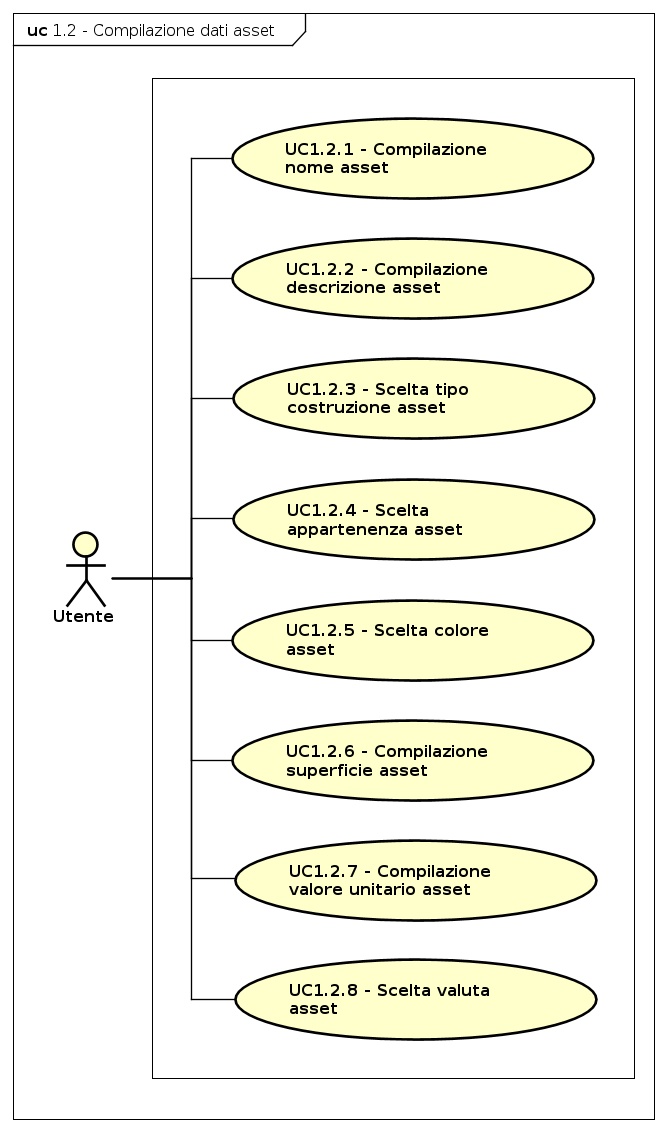
\includegraphics[scale=0.5]{{img/uc1.2}.png} 
	\caption{UC1.2 - Compilazione dati asset}
\end{figure}
\def\arraystretch{1.5}
\rowcolors{2}{D}{P}
\begin{tabularx}{\textwidth}{l|p{0.7\textwidth}}
	\rowcolor{I} \multicolumn{2}{c}{\color{white}\textbf{UC1.2 - Compilazione dati asset}} \\
	\toprule
	\endhead
	\textbf{Attori} & Utente\\
	\textbf{Descrizione} & l'utente compila i dati dell'asset che sta aggiungendo\\
	\textbf{Pre-condizione} & il sistema offre la possibilità di compilare i dati dell'asset\\
	\textbf{Post-condizione} & l'utente ha compilato i dati dell'asset che sta aggiungendo e viene riportato alla schermata di aggiunta dell'asset\\
	\textbf{Scenario principale} & \vspace{-1.2em}\begin{enumerate}[leftmargin=*,noitemsep,nosep]
		\item \nameref{sssec:UC1.2.1};
		\item \nameref{sssec:UC1.2.2};
		\item \nameref{sssec:UC1.2.3};
		\item \nameref{sssec:UC1.2.4};
		\item \nameref{sssec:UC1.2.5};
		\item \nameref{sssec:UC1.2.6};
		\item \nameref{sssec:UC1.2.7}.
	\end{enumerate}\\
	\textbf{Estensioni} & \vspace{-1.2em}\begin{itemize}[leftmargin=*,noitemsep,nosep]
		\item \nameref{sssec:UC1.3}: l’utente interrompe volontariamente la compilazione dei dati dell'asset
	\end{itemize}\\
	%\textbf{Generalizzazioni} &  \\
	\bottomrule
\end{tabularx}
\subsection{UC1.2.1 - Compilazione nome asset} 
\label{sssec:UC1.2.1} 
\def\arraystretch{1.5}
\rowcolors{2}{D}{P}
\begin{tabularx}{\textwidth}{l|p{0.7\textwidth}}
	\rowcolor{I} \multicolumn{2}{c}{\color{white}\textbf{UC1.2.1 - Compilazione nome asset}} \\
	\toprule
	\endhead
	\textbf{Attori} & Utente\\
	\textbf{Descrizione} & l'utente compila il nome dell'asset\\
	\textbf{Pre-condizione} & il sistema offre la possibilità di compilare il nome dell'asset\\
	\textbf{Post-condizione} & l'utente ha compilato il nome dell'asset e può visualizzare il nome appena compilato sull'area informativa\\
	\textbf{Scenario principale} & \vspace{-1.2em}\begin{enumerate}[leftmargin=*,noitemsep,nosep]
		\item \nameref{sssec:UC1.2.1}.
	\end{enumerate}\\
	%\textbf{Generalizzazioni} &  \\
	\bottomrule
\end{tabularx}
\subsection{UC1.2.2 - Compilazione descrizione asset} 
\label{sssec:UC1.2.2} 
\def\arraystretch{1.5}
\rowcolors{2}{D}{P}
\begin{tabularx}{\textwidth}{l|p{0.7\textwidth}}
	\rowcolor{I} \multicolumn{2}{c}{\color{white}\textbf{UC1.2.2 - Compilazione descrizione asset}} \\
	\toprule
	\endhead
	\textbf{Attori} & Utente\\
	\textbf{Descrizione} & l'utente compila la descrizione dell'asset\\
	\textbf{Pre-condizione} & il sistema offre la possibilità di compilare la descrizione dell'asset\\
	\textbf{Post-condizione} & l'utente ha compilato la descrizione dell'asset e può visualizzare la descrizione appena compilata sull'area informativa\\
	\textbf{Scenario principale} & \vspace{-1.2em}\begin{enumerate}[leftmargin=*,noitemsep,nosep]
		\item \nameref{sssec:UC1.2.2}.
	\end{enumerate}\\
	%\textbf{Generalizzazioni} &  \\
	\bottomrule
\end{tabularx}
\subsection{UC1.2.3 - Scelta tipo costruzione asset} 
\label{sssec:UC1.2.3} 
\def\arraystretch{1.5}
\rowcolors{2}{D}{P}
\begin{tabularx}{\textwidth}{l|p{0.7\textwidth}}
	\rowcolor{I} \multicolumn{2}{c}{\color{white}\textbf{UC1.2.3 - Scelta tipo costruzione asset}} \\
	\toprule
	\endhead
	\textbf{Attori} & Utente\\
	\textbf{Descrizione} & l'utente sceglie il tipo di costruzione dell'asset\\
	\textbf{Pre-condizione} & il sistema offre la possibilità di scegliere il tipo di costruzione dell'asset\\
	\textbf{Post-condizione} & l'utente ha scelto il tipo di costruzione dell'asset e può visualizzare il tipo appena scelto sull'area informativa\\
	\textbf{Scenario principale} & \vspace{-1.2em}\begin{enumerate}[leftmargin=*,noitemsep,nosep]
		\item \nameref{sssec:UC1.2.3}.
	\end{enumerate}\\
	%\textbf{Generalizzazioni} &  \\
	\bottomrule
\end{tabularx}
\subsection{UC1.2.4 - Scelta appartenenza asset} 
\label{sssec:UC1.2.4} 
\def\arraystretch{1.5}
\rowcolors{2}{D}{P}
\begin{tabularx}{\textwidth}{l|p{0.7\textwidth}}
	\rowcolor{I} \multicolumn{2}{c}{\color{white}\textbf{UC1.2.4 - Scelta appartenenza asset}} \\
	\toprule
	\endhead
	\textbf{Attori} & Utente\\
	\textbf{Descrizione} & l'utente sceglie a chi appartiene l'asset\\
	\textbf{Pre-condizione} & il sistema offre la possibilità di scegliere a chi appartiene l'asset\\
	\textbf{Post-condizione} & l'utente ha scelto a chi appartiene l'asset e può visualizzare l'appartenenza appena scelta sull'area informativa\\
	\textbf{Scenario principale} & \vspace{-1.2em}\begin{enumerate}[leftmargin=*,noitemsep,nosep]
		\item \nameref{sssec:UC1.2.4}.
	\end{enumerate}\\
	%\textbf{Generalizzazioni} &  \\
	\bottomrule
\end{tabularx}
\subsection{UC1.2.5 - Scelta colore asset} 
\label{sssec:UC1.2.5} 
\def\arraystretch{1.5}
\rowcolors{2}{D}{P}
\begin{tabularx}{\textwidth}{l|p{0.7\textwidth}}
	\rowcolor{I} \multicolumn{2}{c}{\color{white}\textbf{UC1.2.5 - Scelta colore asset}} \\
	\toprule
	\endhead
	\textbf{Attori} & Utente\\
	\textbf{Descrizione} & l'utente sceglie il colore dell'asset\\
	\textbf{Pre-condizione} & il sistema offre la possibilità di scegliere il colore dell'asset\\
	\textbf{Post-condizione} & l'utente ha scelto il colore dell'asset e può visualizzare il colore appena scelto sull'area informativa\\
	\textbf{Scenario principale} & \vspace{-1.2em}\begin{enumerate}[leftmargin=*,noitemsep,nosep]
		\item \nameref{sssec:UC1.2.5}.
	\end{enumerate}\\
	%\textbf{Generalizzazioni} &  \\
	\bottomrule
\end{tabularx}
\subsection{UC1.2.6 - Compilazione superficie asset} 
\label{sssec:UC1.2.6} 
\def\arraystretch{1.5}
\rowcolors{2}{D}{P}
\begin{tabularx}{\textwidth}{l|p{0.7\textwidth}}
	\rowcolor{I} \multicolumn{2}{c}{\color{white}\textbf{UC1.2.6 - Compilazione superficie asset}} \\
	\toprule
	\endhead
	\textbf{Attori} & Utente\\
	\textbf{Descrizione} & l'utente compila la superficie dell'asset\\
	\textbf{Pre-condizione} & il sistema offre la possibilità di compilare la superficie dell'asset\\
	\textbf{Post-condizione} & l'utente ha compilato la superficie dell'asset e può visualizzare la superficie appena compilata sull'area informativa\\
	\textbf{Scenario principale} & \vspace{-1.2em}\begin{enumerate}[leftmargin=*,noitemsep,nosep]
		\item \nameref{sssec:UC1.2.6}.
	\end{enumerate}\\
	%\textbf{Generalizzazioni} &  \\
	\bottomrule
\end{tabularx}
\subsection{UC1.2.7 - Compilazione valore unitario asset} 
\label{sssec:UC1.2.7} 
\def\arraystretch{1.5}
\rowcolors{2}{D}{P}
\begin{tabularx}{\textwidth}{l|p{0.7\textwidth}}
	\rowcolor{I} \multicolumn{2}{c}{\color{white}\textbf{UC1.2.7 - Compilazione valore unitario asset}} \\
	\toprule
	\endhead
	\textbf{Attori} & Utente\\
	\textbf{Descrizione} & l'utente compila il valore unitario dell'asset\\
	\textbf{Pre-condizione} & il sistema offre la possibilità di compilare il valore unitario dell'asset\\
	\textbf{Post-condizione} & l'utente ha compilato il valore unitario dell'asset e può visualizzare il valore appena compilato sull'area informativa\\
	\textbf{Scenario principale} & \vspace{-1.2em}\begin{enumerate}[leftmargin=*,noitemsep,nosep]
		\item \nameref{sssec:UC1.2.7}.
	\end{enumerate}\\
	%\textbf{Generalizzazioni} &  \\
	\bottomrule
\end{tabularx}
\subsection{UC1.3 - Interruzione compilazione dati asset} 
\label{sssec:UC1.3} 
\def\arraystretch{1.5}
\rowcolors{2}{D}{P}
\begin{tabularx}{\textwidth}{l|p{0.7\textwidth}}
	\rowcolor{I} \multicolumn{2}{c}{\color{white}\textbf{UC1.3 - Interruzione compilazione dati asset}} \\
	\toprule
	\endhead
	\textbf{Attori} & Utente\\
	\textbf{Descrizione} & l'utente interrompe la compilazione dei dati dell'asset\\
	\textbf{Pre-condizione} & il sistema offre la possibilità di compilare i dati dell'asset\\
	\textbf{Post-condizione} & i dati dell'asset non sono stati compilati; l'utente viene riportato alla fase di disegno dell'asset\\
	\textbf{Scenario principale} & \vspace{-1.2em}\begin{enumerate}[leftmargin=*,noitemsep,nosep]
		\item \nameref{sssec:UC1.3}.
	\end{enumerate}\\
	%\textbf{Generalizzazioni} &  \\
	\bottomrule
\end{tabularx}
\subsection{UC1.4 - Conferma aggiunta asset} 
\label{sssec:UC1.4} 
\def\arraystretch{1.5}
\rowcolors{2}{D}{P}
\begin{tabularx}{\textwidth}{l|p{0.7\textwidth}}
	\rowcolor{I} \multicolumn{2}{c}{\color{white}\textbf{UC1.4 - Conferma aggiunta asset}} \\
	\toprule
	\endhead
	\textbf{Attori} & Utente\\
	\textbf{Descrizione} & l'utente conferma l'aggiunta dell'asset\\
	\textbf{Pre-condizione} & il sistema offre la possibilità di confermare l'aggiunta dell'asset\\
	\textbf{Post-condizione} & un nuovo asset è stato aggiunto ed è visualizzabile sulla mappa; l'utente visualizza un messaggio che comunica la corretta esecuzione dell'operazione; l'area informativa rimane impostata sull'asset appena inserito; la posizione e il livello di ingrandimento della mappa rimangono invariati\\
	\textbf{Scenario principale} & \vspace{-1.2em}\begin{enumerate}[leftmargin=*,noitemsep,nosep]
		\item \nameref{sssec:UC1.4}.
	\end{enumerate}\\
	\textbf{Estensioni} & \vspace{-1.2em}\begin{itemize}[leftmargin=*,noitemsep,nosep]
		\item \nameref{sssec:UC1.5}: dati inseriti non validi:
		\begin{itemize}
			\item nome vuoto; più lungo di 50 caratteri;
			inizia e/o finisce con uno spazio; contiene caratteri speciali
			\item descrizione vuota; più lunga di 5000
			caratteri; inizia e/o finisce con uno spazio; contiene caratteri
			speciali diversi dall'apostrofo;
			\item tipo di costruzione non scelto;
			\item appartenenza non scelta;
			\item colore non scelto;
			\item superficie (in mq) vuota; più lunga di
			5 cifre per la parte intera; più di 2 per la parte decimale;
			\item valore unitario (monetario) vuoto; più
			lungo di 20 cifre per la parte intera; più di 2 per la parte
			decimale;
			\item valuta non scelta.
		\end{itemize}
	\end{itemize}\\
	%\textbf{Generalizzazioni} &  \\
	\bottomrule
\end{tabularx}
\subsection{UC1.5 - Visualizzazione errore aggiunta asset} 
\label{sssec:UC1.5} 
\def\arraystretch{1.5}
\rowcolors{2}{D}{P}
\begin{tabularx}{\textwidth}{l|p{0.7\textwidth}}
	\rowcolor{I} \multicolumn{2}{c}{\color{white}\textbf{UC1.5 - Visualizzazione errore aggiunta asset}} \\
	\toprule
	\endhead
	\textbf{Attori} & Utente\\
	\textbf{Descrizione} & l'utente visualizza un errore relativo ai dati dell'asset compilati in modo errato\\
	\textbf{Pre-condizione} & l'utente sta tentando di inserire un nuovo asset\\
	\textbf{Post-condizione} & nessun nuovo asset inserito; l'utente visualizza un errore relativo ai dati dell'asset compilati in modo errato; l'utente viene riportato alla schermata di aggiunta asset\\
	\textbf{Scenario principale} & \vspace{-1.2em}\begin{enumerate}[leftmargin=*,noitemsep,nosep]
		\item \nameref{sssec:UC1.5}.
	\end{enumerate}\\
	%\textbf{Generalizzazioni} &  \\
	\bottomrule
\end{tabularx}

\subsection{UC2 - Visualizzazione info asset} 
\label{sssec:UC2} 
\def\arraystretch{1.5}
\rowcolors{2}{D}{P}
\begin{tabularx}{\textwidth}{l|p{0.7\textwidth}}
	\rowcolor{I} \multicolumn{2}{c}{\color{white}\textbf{UC2 - Visualizzazione info asset}} \\
	\toprule
	\endhead
	\textbf{Attori} & Utente\\
	\textbf{Descrizione} & l'utente seleziona un asset e ne visualizza le informazioni\\
	\textbf{Pre-condizione} & l'utente ha aperto l'applicazione, è stato inserito almeno un asset\\
	\textbf{Post-condizione} & il sistema mostra nell'area informativa le informazioni dell'asset selezionato; la posizione e il livello di ingrandimento della mappa rimangono invariati\\
	\textbf{Scenario principale} & \vspace{-1.2em}\begin{enumerate}[leftmargin=*,noitemsep,nosep]
		\item \nameref{sssec:UC2}.
	\end{enumerate}\\
	%\textbf{Generalizzazioni} &  \\
	\bottomrule
\end{tabularx}

\subsection{UC3 - Chiusura visualizzazione info asset} 
\label{sssec:UC3} 
\def\arraystretch{1.5}
\rowcolors{2}{D}{P}
\begin{tabularx}{\textwidth}{l|p{0.7\textwidth}}
	\rowcolor{I} \multicolumn{2}{c}{\color{white}\textbf{UC3 - Chiusura visualizzazione info asset}} \\
	\toprule
	\endhead
	\textbf{Attori} & Utente\\
	\textbf{Descrizione} & l'utente chiude la visualizzazione delle informazioni di un asset\\
	\textbf{Pre-condizione} & l'utente ha visualizzato le informazioni di un asset\\
	\textbf{Post-condizione} & è stata chiusa la visualizzazione delle informazioni dell'asset selezionato nell'area informativa; l'area informativa viene impostata sulla visualizzazione di default; la posizione e il livello di ingrandimento della mappa rimangono invariati\\
	\textbf{Scenario principale} & \vspace{-1.2em}\begin{enumerate}[leftmargin=*,noitemsep,nosep]
		\item \nameref{sssec:UC3}.
	\end{enumerate}\\
	%\textbf{Generalizzazioni} &  \\
	\bottomrule
\end{tabularx}

\subsection{UC4 - Modifica asset} 
\label{sssec:UC4} 
\begin{figure}[H] 
	\centering 
	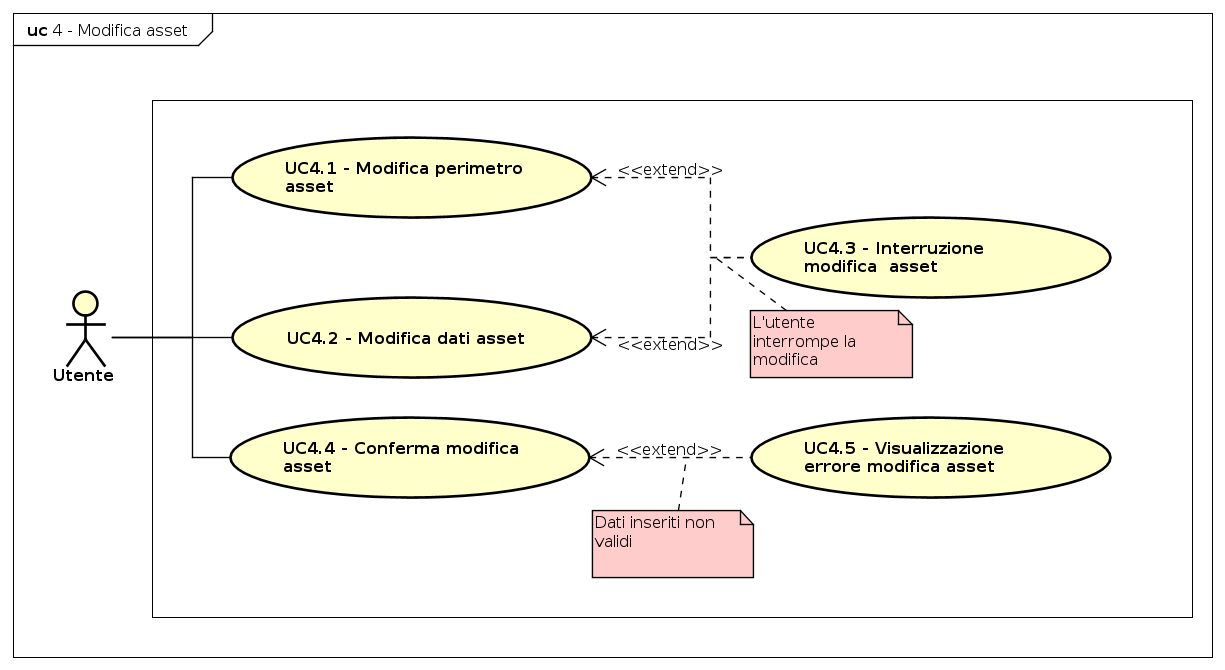
\includegraphics[width=\textwidth]{{img/uc4}.png} 
	\caption{UC4 - Modifica asset}
\end{figure}
\def\arraystretch{1.5}
\rowcolors{2}{D}{P}
\begin{tabularx}{\textwidth}{l|p{0.7\textwidth}}
	\rowcolor{I} \multicolumn{2}{c}{\color{white}\textbf{UC4 - Modifica asset}} \\
	\toprule
	\endhead
	\textbf{Attori} & Utente\\
	\textbf{Descrizione} & l'utente modifica l'asset\\
	\textbf{Pre-condizione} & l'utente ha aperto l'applicazione; almeno un asset è stato aggiunto; l'utente ha selezionato un asset\\
	\textbf{Post-condizione} & l'asset è stato modificato; l'utente visualizza un messaggio che comunica la corretta esecuzione dell'operazione; l'area informativa rimane impostata sull'asset appena modificato; la posizione e il livello di ingrandimento della mappa rimangono invariati\\
	\textbf{Scenario principale} & \vspace{-1.2em}\begin{enumerate}[leftmargin=*,noitemsep,nosep]
		\item \nameref{sssec:UC4.1};
		\item \nameref{sssec:UC4.2};
		\item \nameref{sssec:UC4.3}.
	\end{enumerate}\\
	\textbf{Estensioni} & \vspace{-1.2em}\begin{itemize}[leftmargin=*,noitemsep,nosep]
		\item \nameref{sssec:UC31}: l’utente interrompe volontariamente la modifica dell’asset;
	\end{itemize}\\
	\textbf{Scenari alternativi} & \vspace{-1.2em}\begin{itemize}[leftmargin=*,noitemsep,nosep]
		\item \nameref{sssec:UC4.4}.
	\end{itemize}\\
	%\textbf{Generalizzazioni} &  \\
	\bottomrule
\end{tabularx}
\subsection{UC4.1 - Modifica perimetro asset} 
\label{sssec:UC4.1} 
\begin{figure}[H] 
	\centering 
	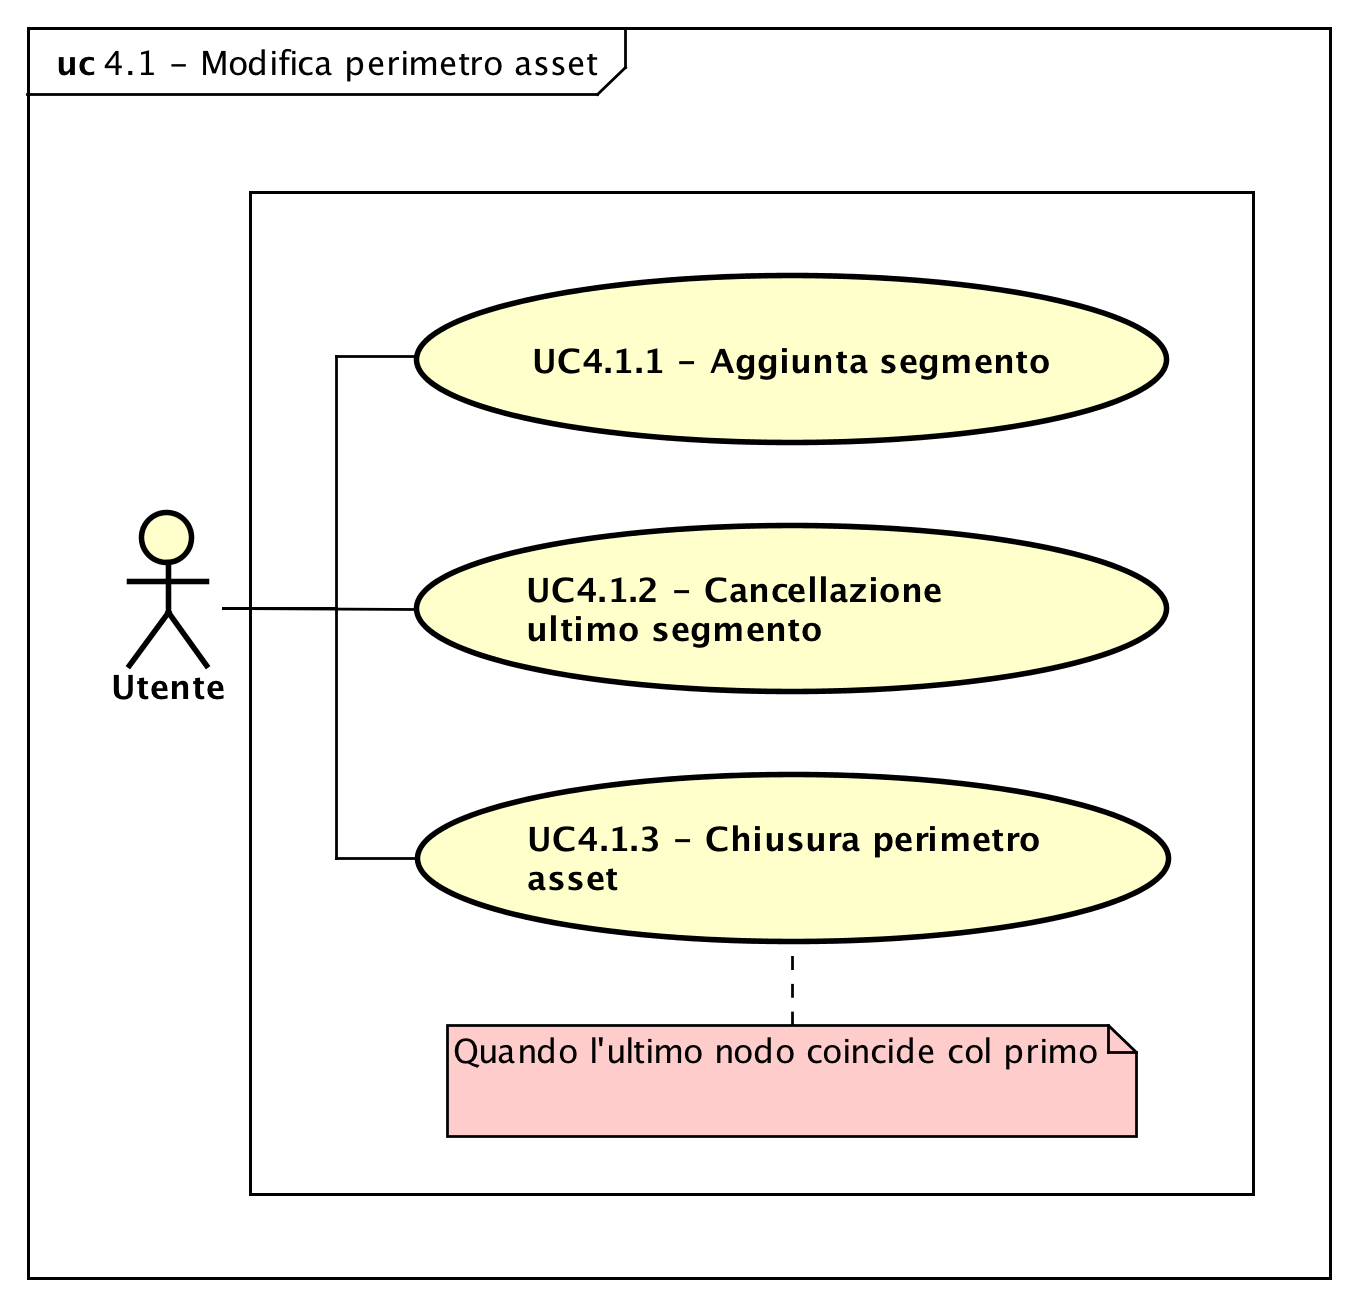
\includegraphics[scale=0.5]{{img/uc4.1}.png} 
	\caption{UC4.1 - Modifica perimetro asset}
\end{figure}
\def\arraystretch{1.5}
\rowcolors{2}{D}{P}
\begin{tabularx}{\textwidth}{l|p{0.7\textwidth}}
	\rowcolor{I} \multicolumn{2}{c}{\color{white}\textbf{UC4.1 - Modifica perimetro asset}} \\
	\toprule
	\endhead
	\textbf{Attori} & Utente\\
	\textbf{Descrizione} & l'utente modifica il perimetro dell'asset\\
	\textbf{Pre-condizione} & il sistema offre la possibilità di modificare il perimetro dell'asset\\
	\textbf{Post-condizione} & il perimetro dell'asset è stato modificato; il nuovo perimetro viene visualizzato sulla mappa; l'utente viene riportato alla schermata di modifica asset\\
	\textbf{Scenario principale} & \vspace{-1.2em}\begin{enumerate}[leftmargin=*,noitemsep,nosep]
		\item \nameref{sssec:UC4.1.1};
		\item \nameref{sssec:UC4.1.2};
		\item \nameref{sssec:UC4.1.3}.
	\end{enumerate}\\
	%\textbf{Generalizzazioni} &  \\
	\bottomrule
\end{tabularx}
\subsection{UC4.1.1 - Aggiunta segmento} 
\label{sssec:UC4.1.1} 
\def\arraystretch{1.5}
\rowcolors{2}{D}{P}
\begin{tabularx}{\textwidth}{l|p{0.7\textwidth}}
	\rowcolor{I} \multicolumn{2}{c}{\color{white}\textbf{UC4.1.1 - Aggiunta segmento}} \\
	\toprule
	\endhead
	\textbf{Attori} & Utente\\
	\textbf{Descrizione} & l'utente aggiunge un segmento al perimetro dell'asset che sta modificando\\
	\textbf{Pre-condizione} & il sistema offre la possibilità di aggiungere un segmento al perimetro dell'asset\\
	\textbf{Post-condizione} & l'utente ha aggiunto un segmento al perimetro dell'asset che sta modificando; il segmento viene visualizzato sulla mappa\\
	\textbf{Scenario principale} & \vspace{-1.2em}\begin{enumerate}[leftmargin=*,noitemsep,nosep]
		\item \nameref{sssec:UC4.1.1}.
	\end{enumerate}\\
	%\textbf{Generalizzazioni} &  \\
	\bottomrule
\end{tabularx}
\subsection{UC4.1.2 - Cancellazione ultimo segmento} 
\label{sssec:UC4.1.2} 
\def\arraystretch{1.5}
\rowcolors{2}{D}{P}
\begin{tabularx}{\textwidth}{l|p{0.7\textwidth}}
	\rowcolor{I} \multicolumn{2}{c}{\color{white}\textbf{UC4.1.2 - Cancellazione ultimo segmento}} \\
	\toprule
	\endhead
	\textbf{Attori} & Utente\\
	\textbf{Descrizione} & l'utente cancella l'ultimo segmento del perimetro dell'asset che sta modificando\\
	\textbf{Pre-condizione} & l'utente sta disegnando il perimetro di un asset; è stato disegnato almeno un segmento\\
	\textbf{Post-condizione} & l'utente ha cancellato l'ultimo segmento del perimetro dell'asset che sta modificando; il segmento non è più visibile sulla mappa\\
	\textbf{Scenario principale} & \vspace{-1.2em}\begin{enumerate}[leftmargin=*,noitemsep,nosep]
		\item \nameref{sssec:UC4.1.2}.
	\end{enumerate}\\
	%\textbf{Generalizzazioni} &  \\
	\bottomrule
\end{tabularx}
\subsection{UC4.1.3 - Chiusura perimetro asset} 
\label{sssec:UC4.1.3} 
\def\arraystretch{1.5}
\rowcolors{2}{D}{P}
\begin{tabularx}{\textwidth}{l|p{0.7\textwidth}}
	\rowcolor{I} \multicolumn{2}{c}{\color{white}\textbf{UC4.1.3 - Chiusura perimetro asset}} \\
	\toprule
	\endhead
	\textbf{Attori} & Utente\\
	\textbf{Descrizione} & l'utente termina di disegnare il perimetro dell'asset che sta modificando, facendo coincidere ultimo e primo nodo\\
	\textbf{Pre-condizione} & il sistema offre la possibilità di disegnare il perimetro dell'asset; l'utente ha disegnato almeno due segmenti\\
	\textbf{Post-condizione} & l'utente ha terminato di disegnare il perimetro di un asset; il perimetro è visualizzato sulla mappa; l'utente può continuare a procedere con la modifica degli altri dati dell'asset sull'area informativa\\
	\textbf{Scenario principale} & \vspace{-1.2em}\begin{enumerate}[leftmargin=*,noitemsep,nosep]
		\item \nameref{sssec:UC4.1.3}.
	\end{enumerate}\\
	%\textbf{Generalizzazioni} &  \\
	\bottomrule
\end{tabularx}
\subsection{UC4.2 - Modifica dati asset} 
\label{sssec:UC4.2} 
\begin{figure}[H] 
	\centering 
	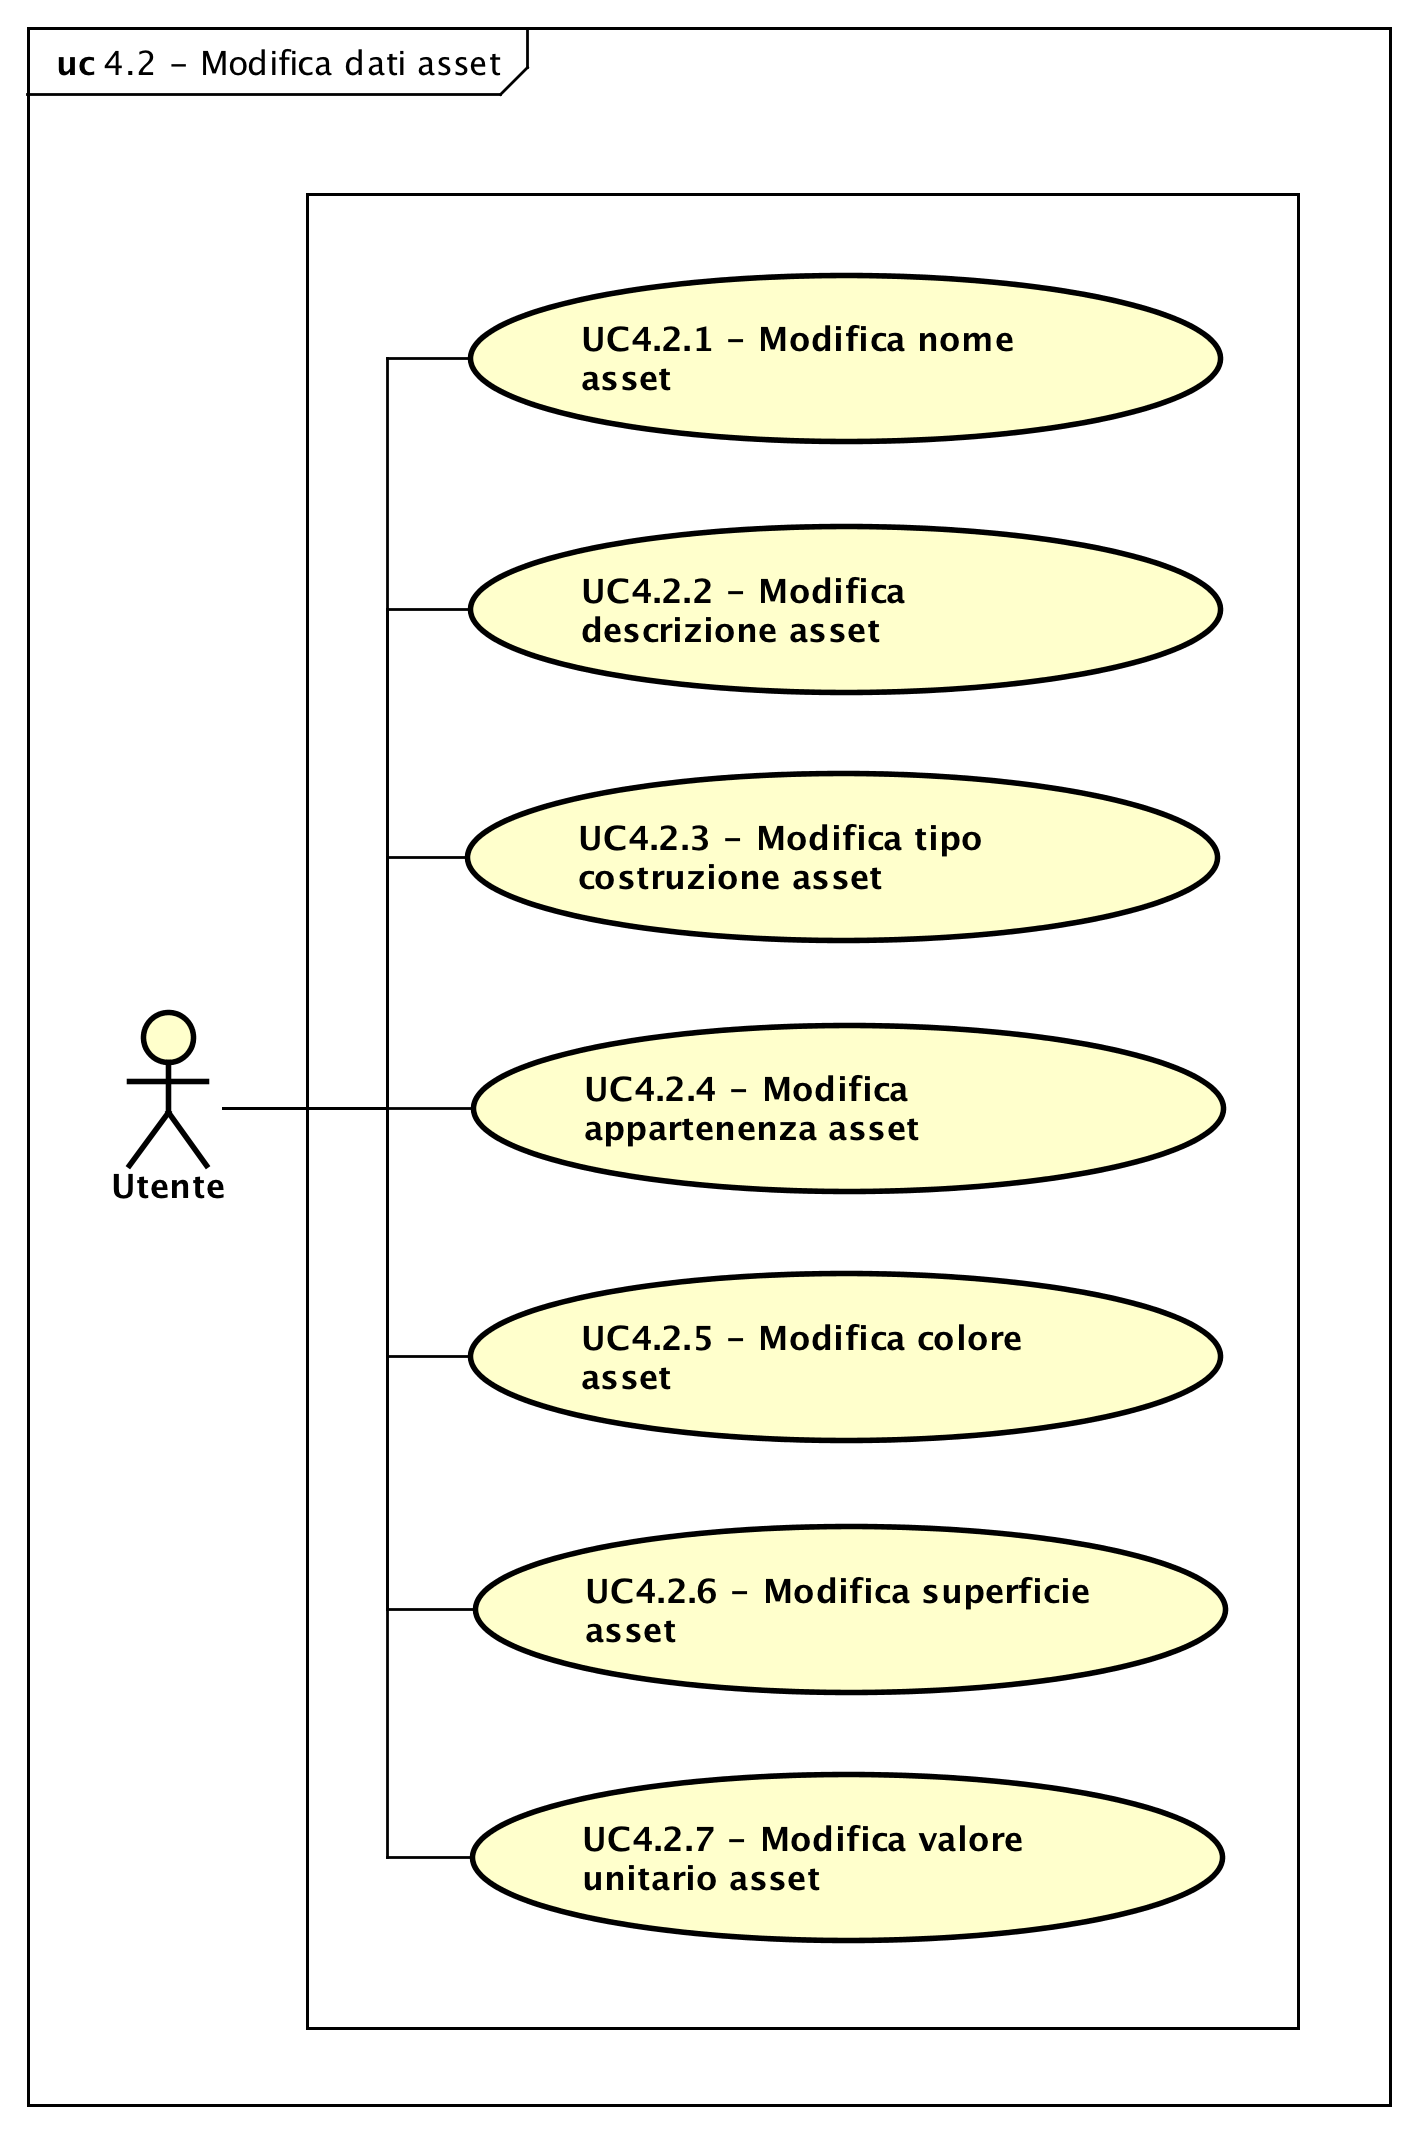
\includegraphics[scale=0.5]{{img/uc4.2}.png} 
	\caption{UC4.2 - Modifica dati asset}
\end{figure}
\def\arraystretch{1.5}
\rowcolors{2}{D}{P}
\begin{tabularx}{\textwidth}{l|p{0.7\textwidth}}
	\rowcolor{I} \multicolumn{2}{c}{\color{white}\textbf{UC4.2 - Modifica dati asset}} \\
	\toprule
	\endhead
	\textbf{Attori} & Utente\\
	\textbf{Descrizione} & l'utente modifica i dati dell'asset\\
	\textbf{Pre-condizione} & il sistema offre la possibilità di modificare i dati dell'asset\\
	\textbf{Post-condizione} & i dati dell'asset sono stati modificati e viene riportato alla schermata di modifica dell'asset\\
	\textbf{Scenario principale} & \vspace{-1.2em}\begin{enumerate}[leftmargin=*,noitemsep,nosep]
		\item \nameref{sssec:UC4.2.1};
		\item \nameref{sssec:UC4.2.2};
		\item \nameref{sssec:UC4.2.3};
		\item \nameref{sssec:UC4.2.4};
		\item \nameref{sssec:UC4.2.5};
		\item \nameref{sssec:UC4.2.6};
		\item \nameref{sssec:UC4.2.7};
		\item \nameref{sssec:UC4.2.8}.
	\end{enumerate}\\
	%\textbf{Generalizzazioni} &  \\
	\bottomrule
\end{tabularx}
\subsection{UC4.2.1 - Modifica nome asset} 
\label{sssec:UC4.2.1} 
\def\arraystretch{1.5}
\rowcolors{2}{D}{P}
\begin{tabularx}{\textwidth}{l|p{0.7\textwidth}}
	\rowcolor{I} \multicolumn{2}{c}{\color{white}\textbf{UC4.2.1 - Modifica nome asset}} \\
	\toprule
	\endhead
	\textbf{Attori} & Utente\\
	\textbf{Descrizione} & l'utente modifica il campo relativo al nome dell'asset\\
	\textbf{Pre-condizione} & il sistema offre la possibilità di modificare il nome dell'asset\\
	\textbf{Post-condizione} & il campo relativo al nome dell'asset è stato modificato; l'utente può visualizzare il nome appena compilato sull'area informativa\\
	\textbf{Scenario principale} & \vspace{-1.2em}\begin{enumerate}[leftmargin=*,noitemsep,nosep]
		\item \nameref{sssec:UC4.2.1}.
	\end{enumerate}\\
	%\textbf{Generalizzazioni} &  \\
	\bottomrule
\end{tabularx}
\subsection{UC4.2.2 - Modifica descrizione asset} 
\label{sssec:UC4.2.2} 
\def\arraystretch{1.5}
\rowcolors{2}{D}{P}
\begin{tabularx}{\textwidth}{l|p{0.7\textwidth}}
	\rowcolor{I} \multicolumn{2}{c}{\color{white}\textbf{UC4.2.2 - Modifica descrizione asset}} \\
	\toprule
	\endhead
	\textbf{Attori} & Utente\\
	\textbf{Descrizione} & l'utente modifica il campo relativo alla descrizione dell'asset\\
	\textbf{Pre-condizione} & il sistema offre la possibilità di modificare la descrizione dell'asset\\
	\textbf{Post-condizione} & il campo relativo alla descrizione dell'asset è stato modificato; l'utente può visualizzare la descrizione appena compilata sull'area informativa\\
	\textbf{Scenario principale} & \vspace{-1.2em}\begin{enumerate}[leftmargin=*,noitemsep,nosep]
		\item \nameref{sssec:UC4.2.2}.
	\end{enumerate}\\
	%\textbf{Generalizzazioni} &  \\
	\bottomrule
\end{tabularx}
\subsection{UC4.2.3 - Modifica tipo costruzione asset} 
\label{sssec:UC4.2.3} 
\def\arraystretch{1.5}
\rowcolors{2}{D}{P}
\begin{tabularx}{\textwidth}{l|p{0.7\textwidth}}
	\rowcolor{I} \multicolumn{2}{c}{\color{white}\textbf{UC4.2.3 - Modifica tipo costruzione asset}} \\
	\toprule
	\endhead
	\textbf{Attori} & Utente\\
	\textbf{Descrizione} & l'utente modifica la scelta relativa al tipo di costruzione dell'asset\\
	\textbf{Pre-condizione} & il sistema offre la possibilità di modificare il tipo di costruzione dell'asset\\
	\textbf{Post-condizione} & la scelta relativa al tipo di costruzione dell'asset è stata modificata; l'utente può visualizzare la scelta appena effettuata sull'area informativa\\
	\textbf{Scenario principale} & \vspace{-1.2em}\begin{enumerate}[leftmargin=*,noitemsep,nosep]
		\item \nameref{sssec:UC4.2.3}.
	\end{enumerate}\\
	%\textbf{Generalizzazioni} &  \\
	\bottomrule
\end{tabularx}
\subsection{UC4.2.4 - Modifica appartenenza asset} 
\label{sssec:UC4.2.4} 
\def\arraystretch{1.5}
\rowcolors{2}{D}{P}
\begin{tabularx}{\textwidth}{l|p{0.7\textwidth}}
	\rowcolor{I} \multicolumn{2}{c}{\color{white}\textbf{UC4.2.4 - Modifica appartenenza asset}} \\
	\toprule
	\endhead
	\textbf{Attori} & Utente\\
	\textbf{Descrizione} & l'utente modifica la scelta relativa al proprietario dell'asset\\
	\textbf{Pre-condizione} & il sistema offre la possibilità di modificare l'appartenenza dell'asset\\
	\textbf{Post-condizione} & la scelta relativa la proprietario dell'asset è stata modificata; l'utente può visualizzare la scelta appena effettuata sull'area informativa\\
	\textbf{Scenario principale} & \vspace{-1.2em}\begin{enumerate}[leftmargin=*,noitemsep,nosep]
		\item \nameref{sssec:UC4.2.4}.
	\end{enumerate}\\
	%\textbf{Generalizzazioni} &  \\
	\bottomrule
\end{tabularx}
\subsection{UC4.2.5 - Modifica colore asset} 
\label{sssec:UC4.2.5} 
\def\arraystretch{1.5}
\rowcolors{2}{D}{P}
\begin{tabularx}{\textwidth}{l|p{0.7\textwidth}}
	\rowcolor{I} \multicolumn{2}{c}{\color{white}\textbf{UC4.2.5 - Modifica colore asset}} \\
	\toprule
	\endhead
	\textbf{Attori} & Utente\\
	\textbf{Descrizione} & l'utente modifica la scelta relativa al colore dell'asset\\
	\textbf{Pre-condizione} & il sistema offre la possibilità di modificare il colore dell'asset\\
	\textbf{Post-condizione} & la scelta relativa al colore dell'asset è stata modificata; l'utente può visualizzare il colore appena scelto sull'area informativa\\
	\textbf{Scenario principale} & \vspace{-1.2em}\begin{enumerate}[leftmargin=*,noitemsep,nosep]
		\item \nameref{sssec:UC4.2.5}.
	\end{enumerate}\\
	%\textbf{Generalizzazioni} &  \\
	\bottomrule
\end{tabularx}
\subsection{UC4.2.6 - Modifica superficie asset} 
\label{sssec:UC4.2.6} 
\def\arraystretch{1.5}
\rowcolors{2}{D}{P}
\begin{tabularx}{\textwidth}{l|p{0.7\textwidth}}
	\rowcolor{I} \multicolumn{2}{c}{\color{white}\textbf{UC4.2.6 - Modifica superficie asset}} \\
	\toprule
	\endhead
	\textbf{Attori} & Utente\\
	\textbf{Descrizione} & l'utente modifica il campo relativo alla superficie dell'asset\\
	\textbf{Pre-condizione} & il sistema offre la possibilità di modificare la superficie dell'asset\\
	\textbf{Post-condizione} & il campo relativo alla superficie dell'asset è stato modificato; l'utente può visualizzare la superficie appena compilata sull'area informativa\\
	\textbf{Scenario principale} & \vspace{-1.2em}\begin{enumerate}[leftmargin=*,noitemsep,nosep]
		\item \nameref{sssec:UC4.2.6}.
	\end{enumerate}\\
	%\textbf{Generalizzazioni} &  \\
	\bottomrule
\end{tabularx}
\subsection{UC4.2.7 - Modifica valore unitario asset} 
\label{sssec:UC4.2.7} 
\def\arraystretch{1.5}
\rowcolors{2}{D}{P}
\begin{tabularx}{\textwidth}{l|p{0.7\textwidth}}
	\rowcolor{I} \multicolumn{2}{c}{\color{white}\textbf{UC4.2.7 - Modifica valore unitario asset}} \\
	\toprule
	\endhead
	\textbf{Attori} & Utente\\
	\textbf{Descrizione} & l'utente modifica il campo relativo al valore unitario dell'asset\\
	\textbf{Pre-condizione} & il sistema offre la possibilità di modificare il valore unitario dell'asset\\
	\textbf{Post-condizione} & il campo relativo al valore unitario dell'asset è stato modificato; l'utente può visualizzare il valore unitario appena compilato sull'area informativa\\
	\textbf{Scenario principale} & \vspace{-1.2em}\begin{enumerate}[leftmargin=*,noitemsep,nosep]
		\item \nameref{sssec:UC4.2.7}.
	\end{enumerate}\\
	%\textbf{Generalizzazioni} &  \\
	\bottomrule
\end{tabularx}
\subsection{UC4.3 - Conferma modifica asset} 
\label{sssec:UC4.3} 
\def\arraystretch{1.5}
\rowcolors{2}{D}{P}
\begin{tabularx}{\textwidth}{l|p{0.7\textwidth}}
	\rowcolor{I} \multicolumn{2}{c}{\color{white}\textbf{UC4.3 - Conferma modifica asset}} \\
	\toprule
	\endhead
	\textbf{Attori} & Utente\\
	\textbf{Descrizione} & l'utente conferma la modifica dell'asset\\
	\textbf{Pre-condizione} & il sistema offre la possibilità di confermare la modifica dell'asset\\
	\textbf{Post-condizione} & l'asset è stato modificato; l'utente visualizza un messaggio che comunica la corretta esecuzione dell'operazione; l'area informativa rimane impostata sull'asset appena modificato; la posizione e il livello di ingrandimento della mappa rimangono invariati\\
	\textbf{Scenario principale} & \vspace{-1.2em}\begin{enumerate}[leftmargin=*,noitemsep,nosep]
		\item \nameref{sssec:UC4.3}.
	\end{enumerate}\\
	\textbf{Estensioni} & \vspace{-1.2em}\begin{itemize}[leftmargin=*,noitemsep,nosep]
		\item \nameref{sssec:UC4.4}: dati inseriti non validi:
		\begin{itemize}
			\item nome vuoto; più lungo di 50 caratteri;
			inizia e/o finisce con uno spazio; contiene caratteri speciali;
			\item descrizione vuota; più lunga di 5000
			caratteri; inizia e/o finisce con uno spazio; contiene caratteri
			speciali diversi dall'apostrofo;
			\item tipo di costruzione non scelto;
			\item appartenenza non scelta;
			\item colore non scelto;
			\item superficie (in mq) vuota; più lunga di
			5 cifre per la parte intera; più di 2 per la parte decimale;
			\item valore unitario (monetario) vuoto; più
			lungo di 20 cifre per la parte intera; più di 2 per la parte
			decimale;
			\item valuta non scelta
		\end{itemize}
	\end{itemize}\\
	%\textbf{Generalizzazioni} &  \\
	\bottomrule
\end{tabularx}
\subsection{UC4.4 - Visualizzazione errore modifica asset} 
\label{sssec:UC4.4} 
\def\arraystretch{1.5}
\rowcolors{2}{D}{P}
\begin{tabularx}{\textwidth}{l|p{0.7\textwidth}}
	\rowcolor{I} \multicolumn{2}{c}{\color{white}\textbf{UC4.4 - Visualizzazione errore modifica asset}} \\
	\toprule
	\endhead
	\textbf{Attori} & Utente\\
	\textbf{Descrizione} & l'utente visualizza un errore relativo alla modifica dell'asset\\
	\textbf{Pre-condizione} & l'utente ha confermato la modifica dei dati dell'asset\\
	\textbf{Post-condizione} & l'asset non è stato modificato; l'utente visualizza un errore relativo ai dati dell'asset compilati in modo errato; l'utente viene riportato alla schermata di modifica asset\\
	\textbf{Scenario principale} & \vspace{-1.2em}\begin{enumerate}[leftmargin=*,noitemsep,nosep]
		\item \nameref{sssec:UC4.4}.
	\end{enumerate}\\
	%\textbf{Generalizzazioni} &  \\
	\bottomrule
\end{tabularx}

\subsection{UC5 - Eliminazione asset} 
\label{sssec:UC5} 
\begin{figure}[H] 
	\centering 
	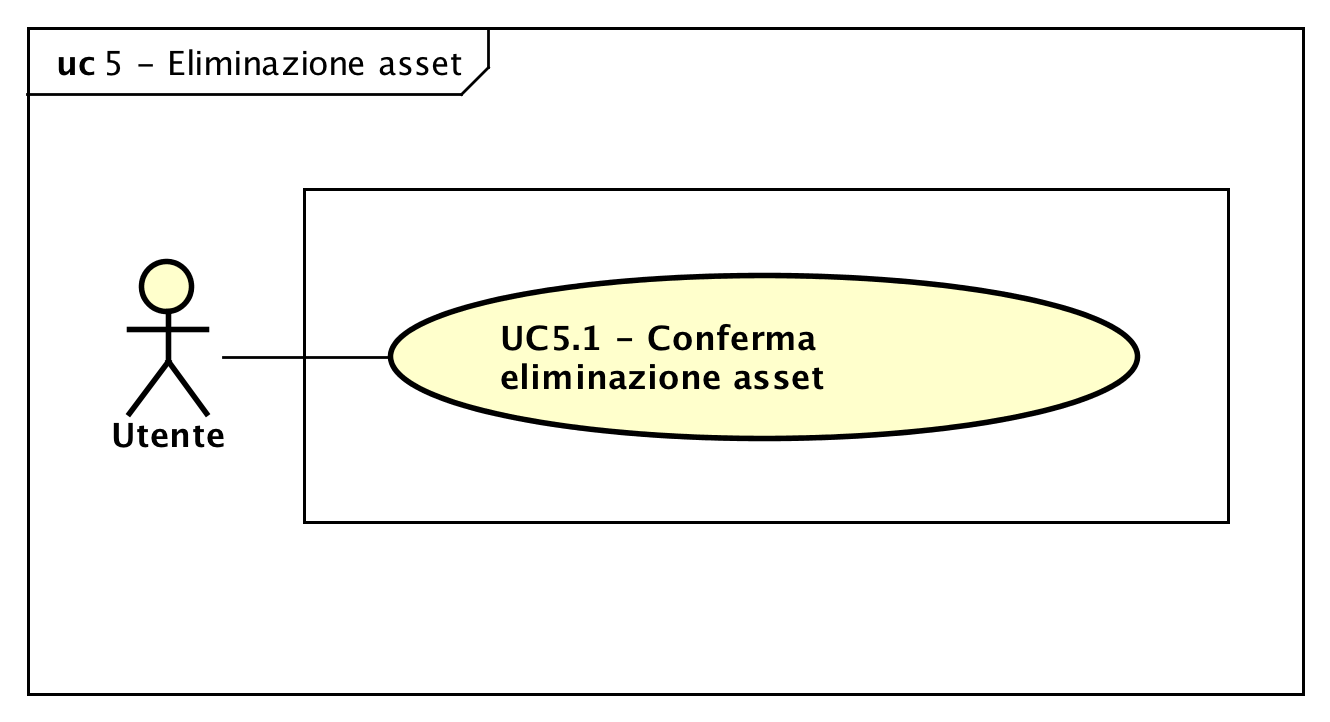
\includegraphics[scale=0.5]{{img/uc5}.png} 
	\caption{UC5 - Eliminazione asset}
\end{figure}
\def\arraystretch{1.5}
\rowcolors{2}{D}{P}
\begin{tabularx}{\textwidth}{l|p{0.7\textwidth}}
	\rowcolor{I} \multicolumn{2}{c}{\color{white}\textbf{UC5 - Eliminazione asset}} \\
	\toprule
	\endhead
	\textbf{Attori} & Utente\\
	\textbf{Descrizione} & l'utente elimina un asset\\
	\textbf{Pre-condizione} & l'utente ha aperto l'applicazione; è stato inserito almeno un asset; l'utente ha selezionato un asset\\
	\textbf{Post-condizione} & l'asset è stato eliminato e non è più visualizzabile sulla mappa; vengono eliminati tutti i nodi contenuti nell'asset; l'utente visualizza un messaggio che comunica la corretta esecuzione dell'operazione; l'area informativa viene impostata sulla visualizzazione di default;  la posizione e il livello di ingrandimento della mappa rimangono invariati\\
	\textbf{Scenario principale} & \vspace{-1.2em}\begin{enumerate}[leftmargin=*,noitemsep,nosep]
		\item \nameref{sssec:UC5.1}.
	\end{enumerate}\\
	\textbf{Estensioni} & \vspace{-1.2em}\begin{itemize}[leftmargin=*,noitemsep,nosep]
		\item \nameref{sssec:UC32}: l'utente interrompe volontariamente l'eliminazione dell'asset.
	\end{itemize}\\
	%\textbf{Generalizzazioni} &  \\
	\bottomrule
\end{tabularx}
\subsection{UC5.1 - Conferma eliminazione asset} 
\label{sssec:UC5.1} 
\def\arraystretch{1.5}
\rowcolors{2}{D}{P}
\begin{tabularx}{\textwidth}{l|p{0.7\textwidth}}
	\rowcolor{I} \multicolumn{2}{c}{\color{white}\textbf{UC5.1 - Conferma eliminazione asset}} \\
	\toprule
	\endhead
	\textbf{Attori} & Utente\\
	\textbf{Descrizione} & l'utente conferma l'eliminazione dell'asset\\
	\textbf{Pre-condizione} & il sistema offre la possibilità di confermare l'eliminazione dell'asset\\
	\textbf{Post-condizione} & l'asset è stato eliminato e non è più visibile sulla mappa; l'utente visualizza un messaggio che comunica la corretta esecuzione dell'operazione;  l'area informativa viene impostata sulla visualizzazione di default; la posizione e il livello di ingrandimento della mappa rimangono invariati\\
	\textbf{Scenario principale} & \vspace{-1.2em}\begin{enumerate}[leftmargin=*,noitemsep,nosep]
		\item \nameref{sssec:UC5.1}.
	\end{enumerate}\\
	%\textbf{Generalizzazioni} &  \\
	\bottomrule
\end{tabularx}
\subsection{UC6 - Aggiunta nodo} 
\label{sssec:UC6} 
\begin{figure}[H] 
	\centering 
	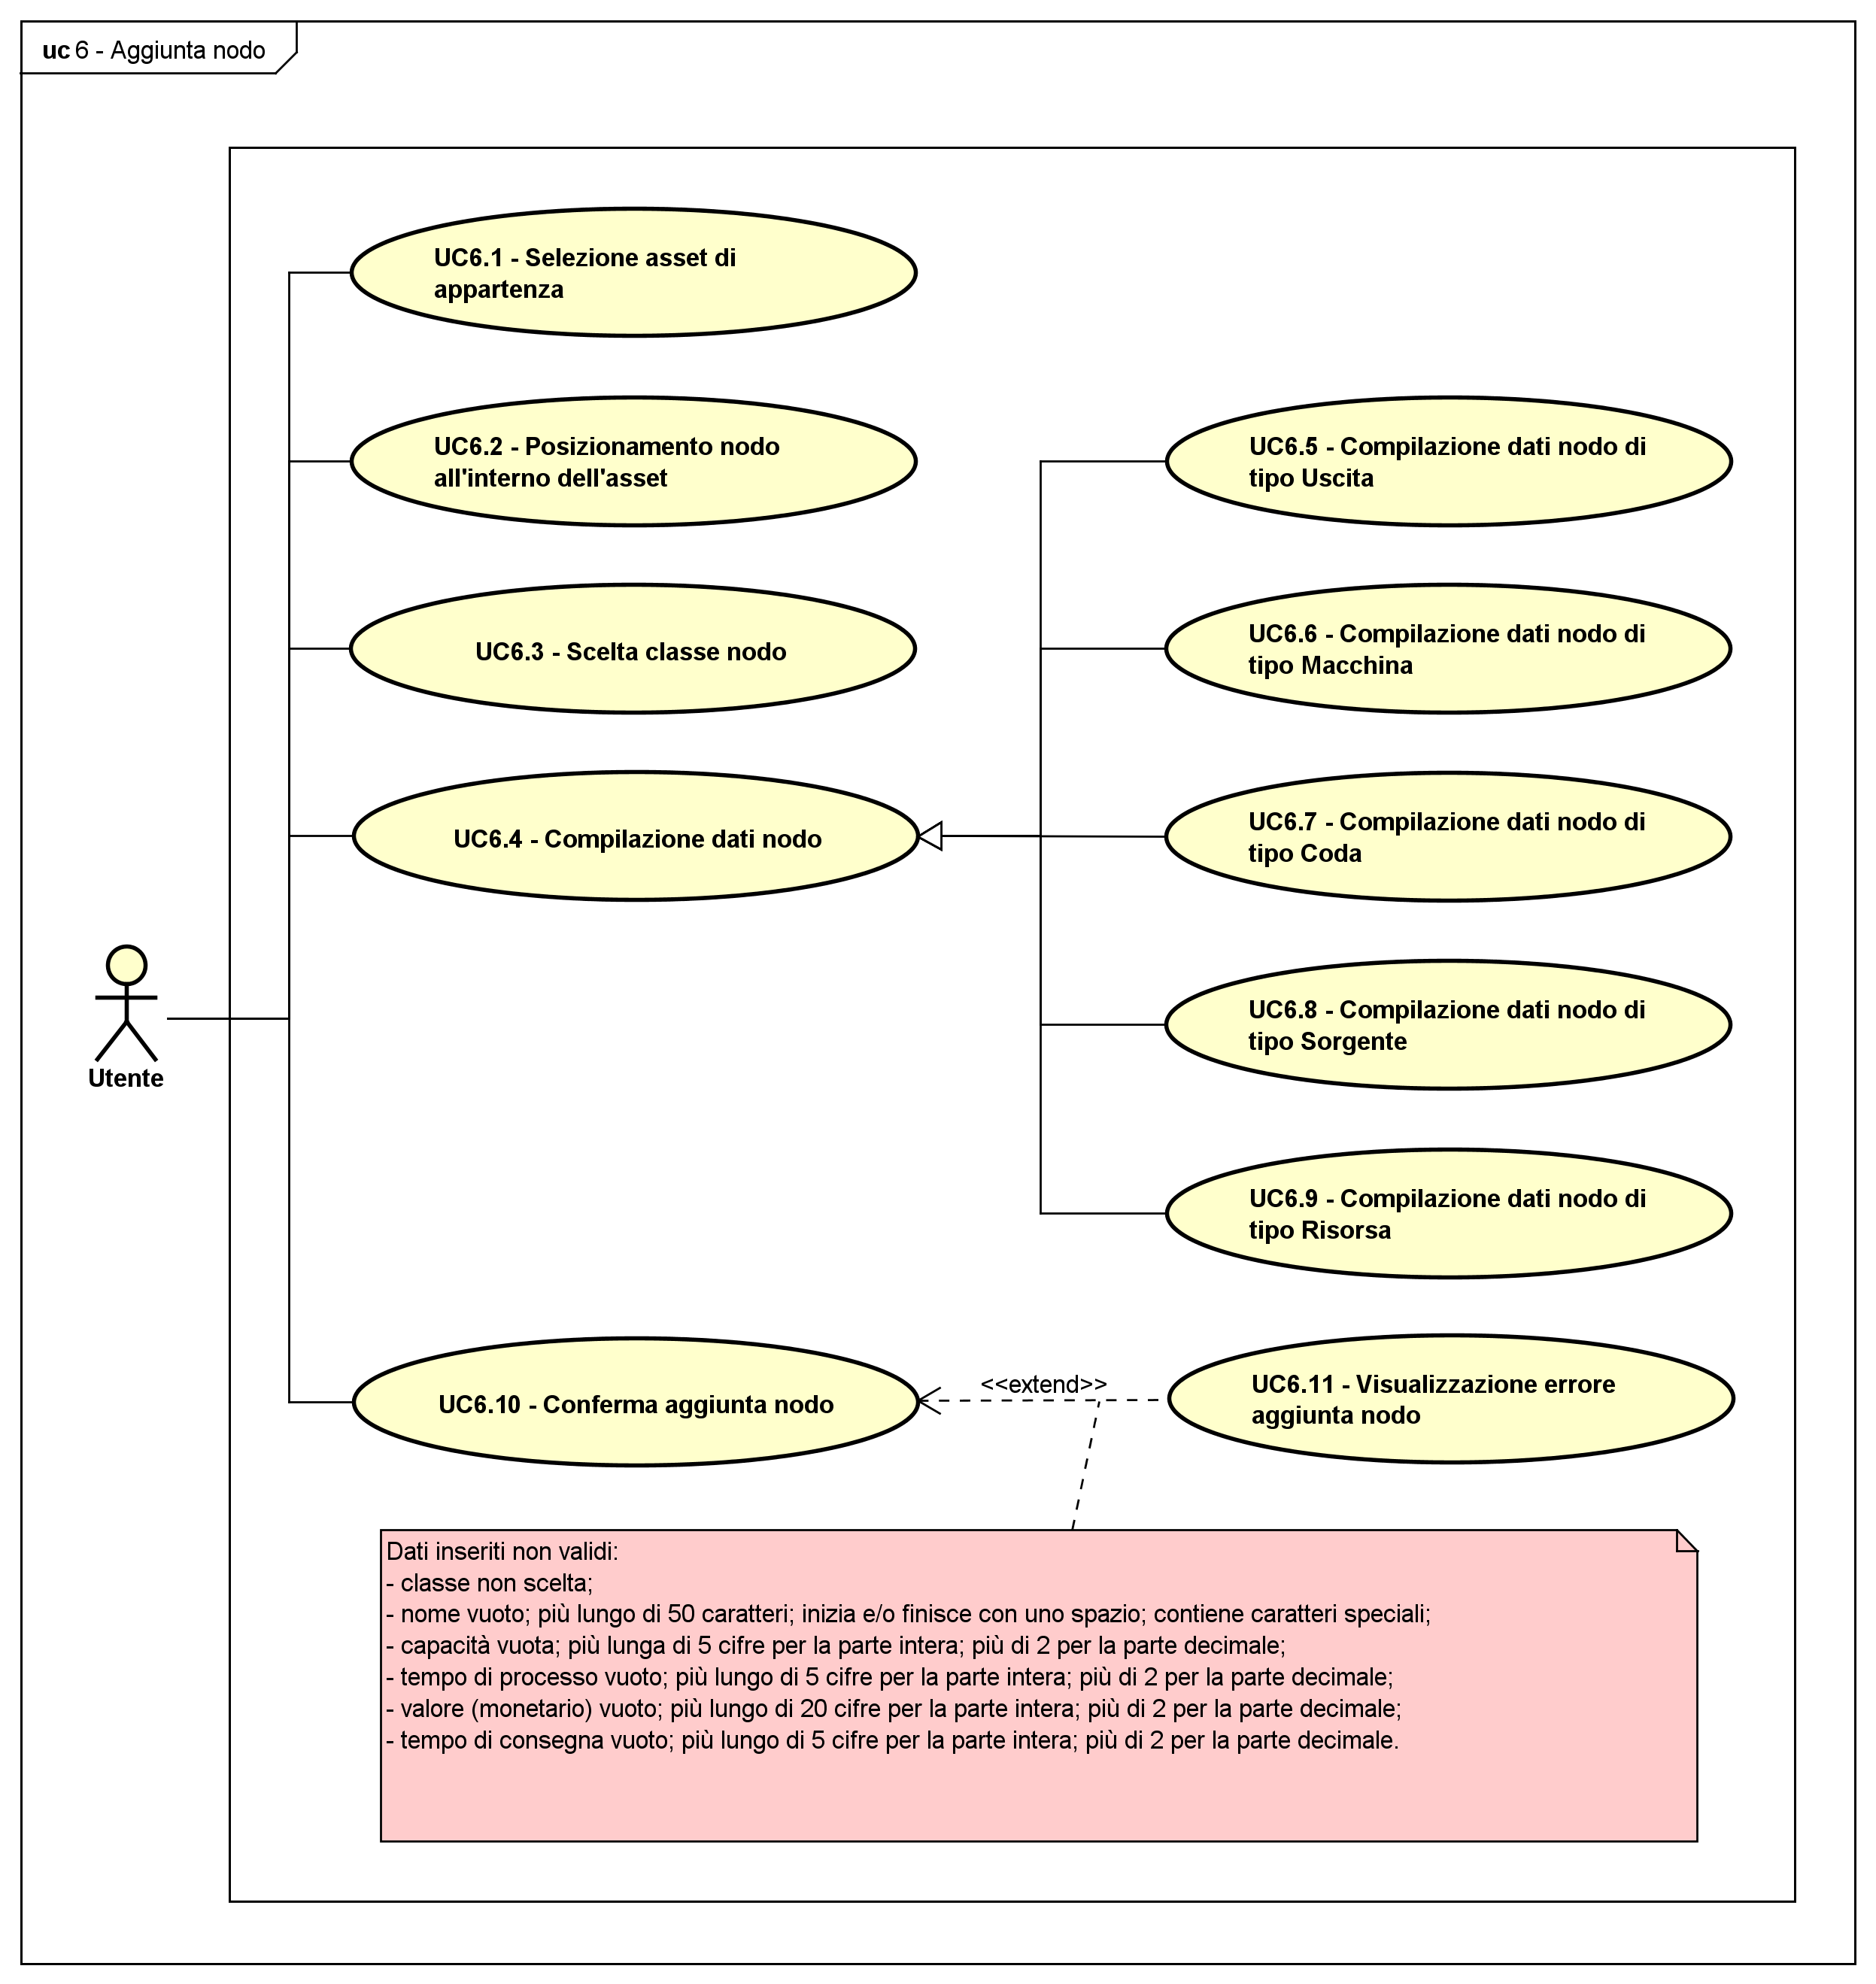
\includegraphics[width=\textwidth]{{img/uc6}.png} 
	\caption{UC6 - Aggiunta nodo}
\end{figure}
\def\arraystretch{1.5}
\rowcolors{2}{D}{P}
\begin{tabularx}{\textwidth}{l|p{0.7\textwidth}}
	\rowcolor{I} \multicolumn{2}{c}{\color{white}\textbf{UC6 - Aggiunta nodo}} \\
	\toprule
	\endhead
	\textbf{Attori} & Utente\\
	\textbf{Descrizione} & l'utente aggiunge un nodo\\
	\textbf{Pre-condizione} & l'utente ha aperto l'applicazione; è stato inserito almeno un asset\\
	\textbf{Post-condizione} & un nuovo nodo è stato aggiunto ed è visualizzabile sulla mappa; l'utente visualizza un messaggio che comunica la corretta esecuzione dell'operazione; l'area informativa rimane impostata sul nodo appena inserito; la posizione e il livello di ingrandimento della mappa rimangono invariati\\
	\textbf{Scenario principale} & \vspace{-1.2em}\begin{enumerate}[leftmargin=*,noitemsep,nosep]
		\item \nameref{sssec:UC6.1};
		\item \nameref{sssec:UC6.2};
		\item \nameref{sssec:UC6.3};
		\item \nameref{sssec:UC6.4};
		\item \nameref{sssec:UC6.5} oppure
		\item \nameref{sssec:UC6.6} oppure
		\item \nameref{sssec:UC6.7} oppure
		\item \nameref{sssec:UC6.8} oppure
		\item \nameref{sssec:UC6.9} oppure
		\item \nameref{sssec:UC6.10}.
	\end{enumerate}\\
	\textbf{Estensioni} & \vspace{-1.2em}\begin{itemize}[leftmargin=*,noitemsep,nosep]
		\item \nameref{sssec:UC33}: l'utente interrompe volontariamente l'aggiunta del nodo.
	\end{itemize}\\
	\textbf{Scenari alternativi} & \vspace{-1.2em}\begin{itemize}[leftmargin=*,noitemsep,nosep]
		\item \nameref{sssec:UC6.11}.
	\end{itemize}\\
	%\textbf{Generalizzazioni} &  \\
	\bottomrule
\end{tabularx}
\subsection{UC6.1 - Selezione asset di appartenenza} 
\label{sssec:UC6.1} 
\def\arraystretch{1.5}
\rowcolors{2}{D}{P}
\begin{tabularx}{\textwidth}{l|p{0.7\textwidth}}
	\rowcolor{I} \multicolumn{2}{c}{\color{white}\textbf{UC6.1 - Selezione asset di appartenenza}} \\
	\toprule
	\endhead
	\textbf{Attori} & Utente\\
	\textbf{Descrizione} & l'utente seleziona un asset\\
	\textbf{Pre-condizione} & il sistema offre la possibilità di selezionare l'asset di appartenenza\\
	\textbf{Post-condizione} & l'asset di appartenenza è stato selezionato; l'utente può continuare a posizionare il nodo e compilare le altre informazioni\\
	\textbf{Scenario principale} & \vspace{-1.2em}\begin{enumerate}[leftmargin=*,noitemsep,nosep]
		\item \nameref{sssec:UC6.1}.
	\end{enumerate}\\
	%\textbf{Generalizzazioni} &  \\
	\bottomrule
\end{tabularx}

\subsection{UC6.2 - Posizionamento nodo all'interno dell'asset} 
\label{sssec:UC6.2} 
\def\arraystretch{1.5}
\rowcolors{2}{D}{P}
\begin{tabularx}{\textwidth}{l|p{0.7\textwidth}}
	\rowcolor{I} \multicolumn{2}{c}{\color{white}\textbf{UC6.2 - Posizionamento nodo all'interno dell'asset}} \\
	\toprule
	\endhead
	\textbf{Attori} & Utente\\
	\textbf{Descrizione} & il sistema offre la possibilità di posizionare il nodo all'interno dell'asset\\
	\textbf{Pre-condizione} & l'utente ha selezionato l'asset di appartenenza\\
	\textbf{Post-condizione} & il nodo è stato posizionato all'interno dell'asset ed è visibile sulla mappa\\
	\textbf{Scenario principale} & \vspace{-1.2em}\begin{enumerate}[leftmargin=*,noitemsep,nosep]
		\item \nameref{sssec:UC6.2}.
	\end{enumerate}\\
	%\textbf{Generalizzazioni} &  \\
	\bottomrule
\end{tabularx}
\subsection{UC6.3 - Scelta classe nodo} 
\label{sssec:UC6.3} 
\def\arraystretch{1.5}
\rowcolors{2}{D}{P}
\begin{tabularx}{\textwidth}{l|p{0.7\textwidth}}
	\rowcolor{I} \multicolumn{2}{c}{\color{white}\textbf{UC6.3 - Scelta classe nodo}} \\
	\toprule
	\endhead
	\textbf{Attori} & Utente\\
	\textbf{Descrizione} & il sistema offre la possibilità di scegliere la classe del nodo\\
	\textbf{Pre-condizione} & l'utente ha posizionato il nodo all'interno dell'asset\\
	\textbf{Post-condizione} & la classe del nodo è stata scelta; la forma del nodo sulla mappa viene cambiata in base alla classe scelta\\
	\textbf{Scenario principale} & \vspace{-1.2em}\begin{enumerate}[leftmargin=*,noitemsep,nosep]
		\item \nameref{sssec:UC6.3}.
	\end{enumerate}\\
	%\textbf{Generalizzazioni} &  \\
	\bottomrule
\end{tabularx}
\subsection{UC6.4 - Compilazione dati nodo} 
\label{sssec:UC6.4} 
\begin{figure}[H] 
	\centering 
	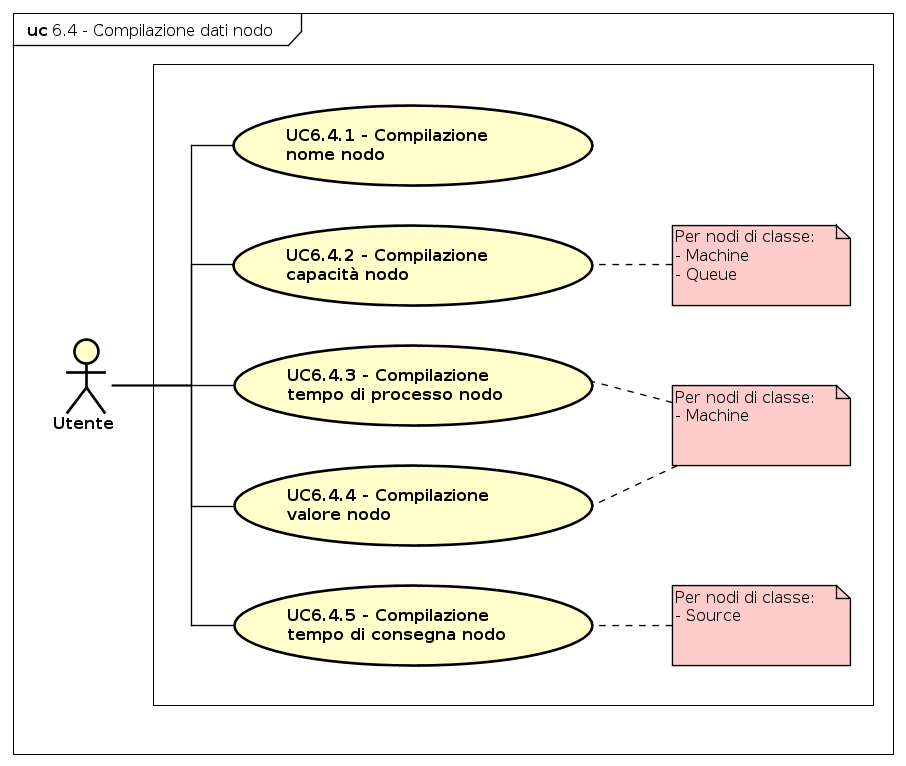
\includegraphics[scale=0.5]{{img/uc6.4}.png} 
	\caption{UC6.4 - Compilazione dati nodo}
\end{figure}
\def\arraystretch{1.5}
\rowcolors{2}{D}{P}
\begin{tabularx}{\textwidth}{l|p{0.7\textwidth}}
	\rowcolor{I} \multicolumn{2}{c}{\color{white}\textbf{UC6.4 - Compilazione dati nodo}} \\
	\toprule
	\endhead
	\textbf{Attori} & Utente\\
	\textbf{Descrizione} & il sistema offre la possibilità di compilare i dati del nodo\\
	\textbf{Pre-condizione} & l'utente ha posizionato il nodo;\\
	\textbf{Post-condizione} & i dati del nodo sono stati compilati; l'utente visualizza i dati appena compilati nell'area informativa\\
	\textbf{Scenario principale} & \vspace{-1.2em}\begin{enumerate}[leftmargin=*,noitemsep,nosep]
		\item \nameref{sssec:UC6.4.1}.
	\end{enumerate}\\
	\textbf{Generalizzazioni} & \vspace{-1.2em}
	\begin{itemize}[leftmargin=*,noitemsep,nosep]
		\item \nameref{sssec:UC6.5};
		\item \nameref{sssec:UC6.6};
		\item \nameref{sssec:UC6.7};
		\item \nameref{sssec:UC6.8};
		\item \nameref{sssec:UC6.9}.
	\end{itemize} \\
	\bottomrule
\end{tabularx}
\subsection{UC6.4.1 - Compilazione nome nodo} 
\label{sssec:UC6.4.1} 
\def\arraystretch{1.5}
\rowcolors{2}{D}{P}
\begin{tabularx}{\textwidth}{l|p{0.7\textwidth}}
	\rowcolor{I} \multicolumn{2}{c}{\color{white}\textbf{UC6.4.1 - Compilazione nome nodo}} \\
	\toprule
	\endhead
	\textbf{Attori} & Utente\\
	\textbf{Descrizione} & l'utente compila il nome del nodo\\
	\textbf{Pre-condizione} & il sistema offre la possibilità di compilare il nome del nodo\\
	\textbf{Post-condizione} & l'utente ha compilato il nome del nodo e visualizza il nome appena compilato nell'area informativa\\
	\textbf{Scenario principale} & \vspace{-1.2em}\begin{enumerate}[leftmargin=*,noitemsep,nosep]
		\item \nameref{sssec:UC6.4.1}.
	\end{enumerate}\\
	%\textbf{Generalizzazioni} &  \\
	\bottomrule
\end{tabularx}
\subsection{UC6.5 - Compilazione dati nodo di tipo Uscita} 
\label{sssec:UC6.5} 
\def\arraystretch{1.5}
\rowcolors{2}{D}{P}
\begin{tabularx}{\textwidth}{l|p{0.7\textwidth}}
	\rowcolor{I} \multicolumn{2}{c}{\color{white}\textbf{UC6.5 - Compilazione dati nodo di tipo Uscita}} \\
	\toprule
	\endhead
	\textbf{Attori} & Utente\\
	\textbf{Descrizione} & l'utente compila i dati del nodo di tipo Uscita\\
	\textbf{Pre-condizione} & l'utente ha posizionato il nodo; l'utente ha scelto come tipologia di nodo Uscita\\
	\textbf{Post-condizione} & i dati del nodo di tipo Uscita sono stati compilati; l'utente visualizza i dati appena compilati nell'area informativa\\
	\textbf{Scenario principale} & \vspace{-1.2em}\begin{enumerate}[leftmargin=*,noitemsep,nosep]
		\item \nameref{sssec:UC6.5}.
	\end{enumerate}\\
	%\textbf{Generalizzazioni} &  \\
	\bottomrule
\end{tabularx}
\subsection{UC6.6 - Compilazione dati nodo di tipo Macchina} 
\label{sssec:UC6.6} 
\begin{figure}[H] 
	\centering 
	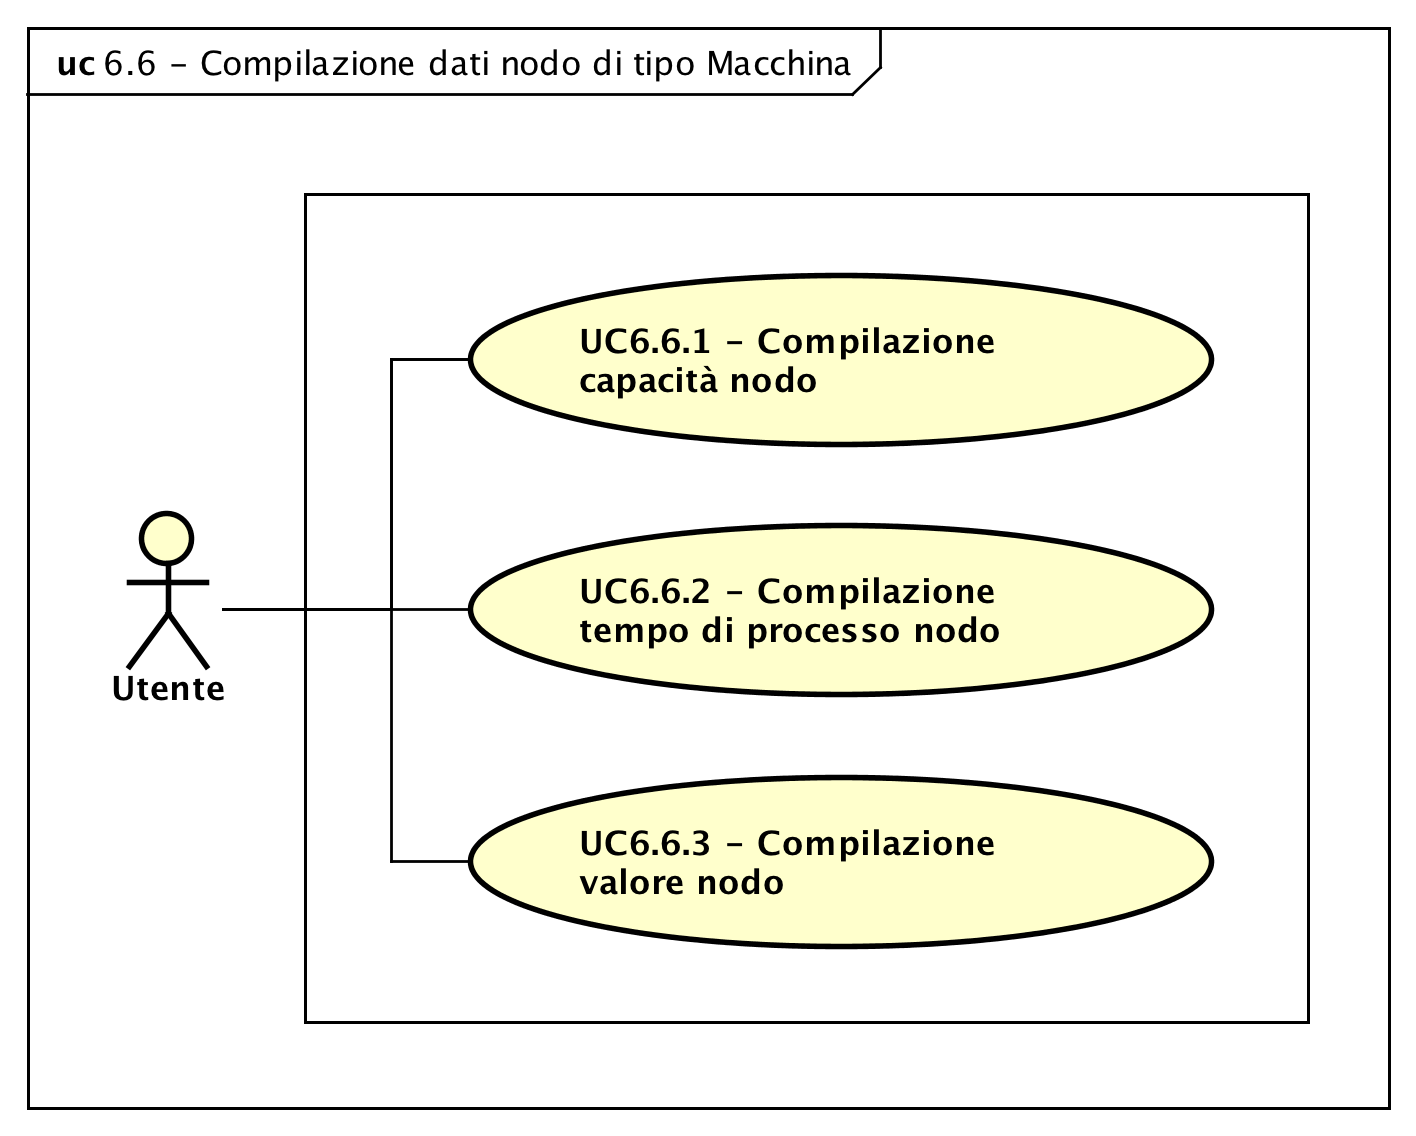
\includegraphics[scale=0.5]{{img/uc6.6}.png} 
	\caption{UC6.6 - Compilazione dati nodo di tipo Macchina}
\end{figure}
\def\arraystretch{1.5}
\rowcolors{2}{D}{P}
\begin{tabularx}{\textwidth}{l|p{0.7\textwidth}}
	\rowcolor{I} \multicolumn{2}{c}{\color{white}\textbf{UC6.6 - Compilazione dati nodo di tipo Macchina}} \\
	\toprule
	\endhead
	\textbf{Attori} & Utente\\
	\textbf{Descrizione} & l'utente compila i dati del nodo di tipo Macchina\\
	\textbf{Pre-condizione} & l'utente ha posizionato il nodo; l'utente ha scelto come tipologia di nodo Macchina\\
	\textbf{Post-condizione} & i dati del nodo di tipo Macchina sono stati compilati; l'utente visualizza i dati appena compilati nell'area informativa\\
	\textbf{Scenario principale} & \vspace{-1.2em}\begin{enumerate}[leftmargin=*,noitemsep,nosep]
		\item \nameref{sssec:UC6.6.1};
		\item \nameref{sssec:UC6.6.2};
		\item \nameref{sssec:UC6.6.3}.
	\end{enumerate}\\
	%\textbf{Generalizzazioni} &  \\
	\bottomrule
\end{tabularx}
\subsection{UC6.6.1 - Compilazione capacità nodo} 
\label{sssec:UC6.6.1} 
\def\arraystretch{1.5}
\rowcolors{2}{D}{P}
\begin{tabularx}{\textwidth}{l|p{0.7\textwidth}}
	\rowcolor{I} \multicolumn{2}{c}{\color{white}\textbf{UC6.6.1 - Compilazione capacità nodo}} \\
	\toprule
	\endhead
	\textbf{Attori} & Utente\\
	\textbf{Descrizione} & l'utente compila la capacità del nodo\\
	\textbf{Pre-condizione} & il sistema offre la possibilità di compilare il nome del nodo; l'utente ha scelto come tipologia di nodo Macchina o Coda\\
	\textbf{Post-condizione} & l'utente ha compilato la capacità del nodo e visualizza la capacità appena compilata nell'area informativa\\
	\textbf{Scenario principale} & \vspace{-1.2em}\begin{enumerate}[leftmargin=*,noitemsep,nosep]
		\item \nameref{sssec:UC6.6.1}.
	\end{enumerate}\\
	%\textbf{Generalizzazioni} &  \\
	\bottomrule
\end{tabularx}
\subsection{UC6.6.2 - Compilazione tempo di processo nodo} 
\label{sssec:UC6.6.2} 
\def\arraystretch{1.5}
\rowcolors{2}{D}{P}
\begin{tabularx}{\textwidth}{l|p{0.7\textwidth}}
	\rowcolor{I} \multicolumn{2}{c}{\color{white}\textbf{UC6.6.2 - Compilazione tempo di processo nodo}} \\
	\toprule
	\endhead
	\textbf{Attori} & Utente\\
	\textbf{Descrizione} & l'utente compila il tempo di processo del nodo\\
	\textbf{Pre-condizione} & il sistema offre la possibilità di compilare il tempo di processo del nodo; l'utente ha scelto come tipologia di nodo Macchina\\
	\textbf{Post-condizione} & l'utente ha compilato il tempo di processo del nodo e visualizza il tempo di processo appena compilato nell'area informativa\\
	\textbf{Scenario principale} & \vspace{-1.2em}\begin{enumerate}[leftmargin=*,noitemsep,nosep]
		\item \nameref{sssec:UC6.6.2}.
	\end{enumerate}\\
	%\textbf{Generalizzazioni} &  \\
	\bottomrule
\end{tabularx}
\subsection{UC6.6.3 - Compilazione valore nodo} 
\label{sssec:UC6.6.3} 
\def\arraystretch{1.5}
\rowcolors{2}{D}{P}
\begin{tabularx}{\textwidth}{l|p{0.7\textwidth}}
	\rowcolor{I} \multicolumn{2}{c}{\color{white}\textbf{UC6.6.3 - Compilazione valore nodo}} \\
	\toprule
	\endhead
	\textbf{Attori} & Utente\\
	\textbf{Descrizione} & l'utente compila il valore del nodo\\
	\textbf{Pre-condizione} & il sistema offre la possibilità di compilare il valore del nodo; l'utente ha scelto come tipologia di nodo Macchina\\
	\textbf{Post-condizione} & l'utente ha compilato il valore del nodo e visualizza il valore appena compilato nell'area informativa\\
	\textbf{Scenario principale} & \vspace{-1.2em}\begin{enumerate}[leftmargin=*,noitemsep,nosep]
		\item \nameref{sssec:UC6.6.3}.
	\end{enumerate}\\
	%\textbf{Generalizzazioni} &  \\
	\bottomrule
\end{tabularx}
\subsection{UC6.7 - Compilazione dati nodo di tipo Coda} 
\label{sssec:UC6.7} 
\begin{figure}[H] 
	\centering 
	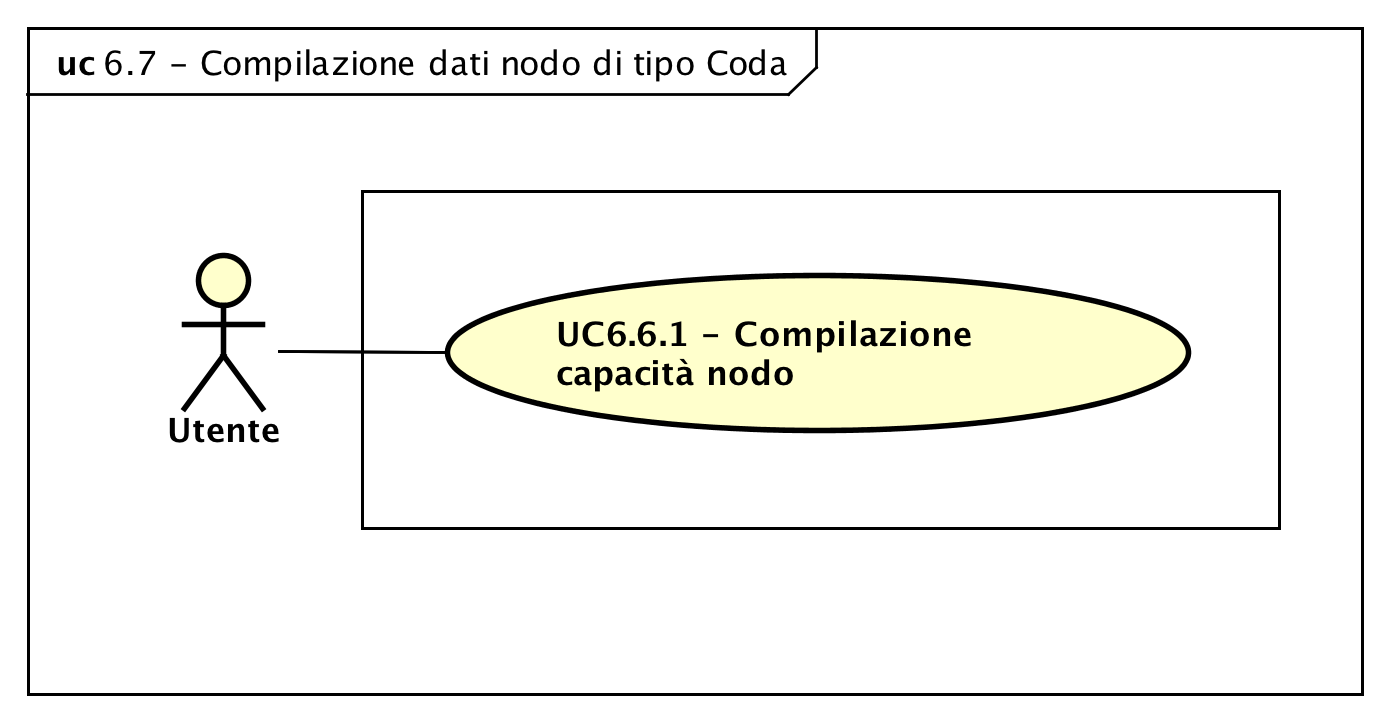
\includegraphics[scale=0.5]{{img/uc6.7}.png} 
	\caption{UC6.7 - Compilazione dati nodo di tipo Coda}
\end{figure}
\def\arraystretch{1.5}
\rowcolors{2}{D}{P}
\begin{tabularx}{\textwidth}{l|p{0.7\textwidth}}
	\rowcolor{I} \multicolumn{2}{c}{\color{white}\textbf{UC6.7 - Compilazione dati nodo di tipo Coda}} \\
	\toprule
	\endhead
	\textbf{Attori} & Utente\\
	\textbf{Descrizione} & l'utente compila i dati del nodo di tipo Coda\\
	\textbf{Pre-condizione} & l'utente ha posizionato il nodo; l'utente ha scelto come tipologia di nodo Coda\\
	\textbf{Post-condizione} & i dati del nodo di tipo Coda sono stati compilati; l'utente visualizza i dati appena compilati nell'area informativa\\
	\textbf{Scenario principale} & \vspace{-1.2em}\begin{enumerate}[leftmargin=*,noitemsep,nosep]
		\item \nameref{sssec:UC6.6.1}.
	\end{enumerate}\\
	%\textbf{Generalizzazioni} &  \\
	\bottomrule
\end{tabularx}
\subsection{UC6.8 - Compilazione dati nodo di tipo Sorgente} 
\label{sssec:UC6.8} 
\begin{figure}[H] 
	\centering 
	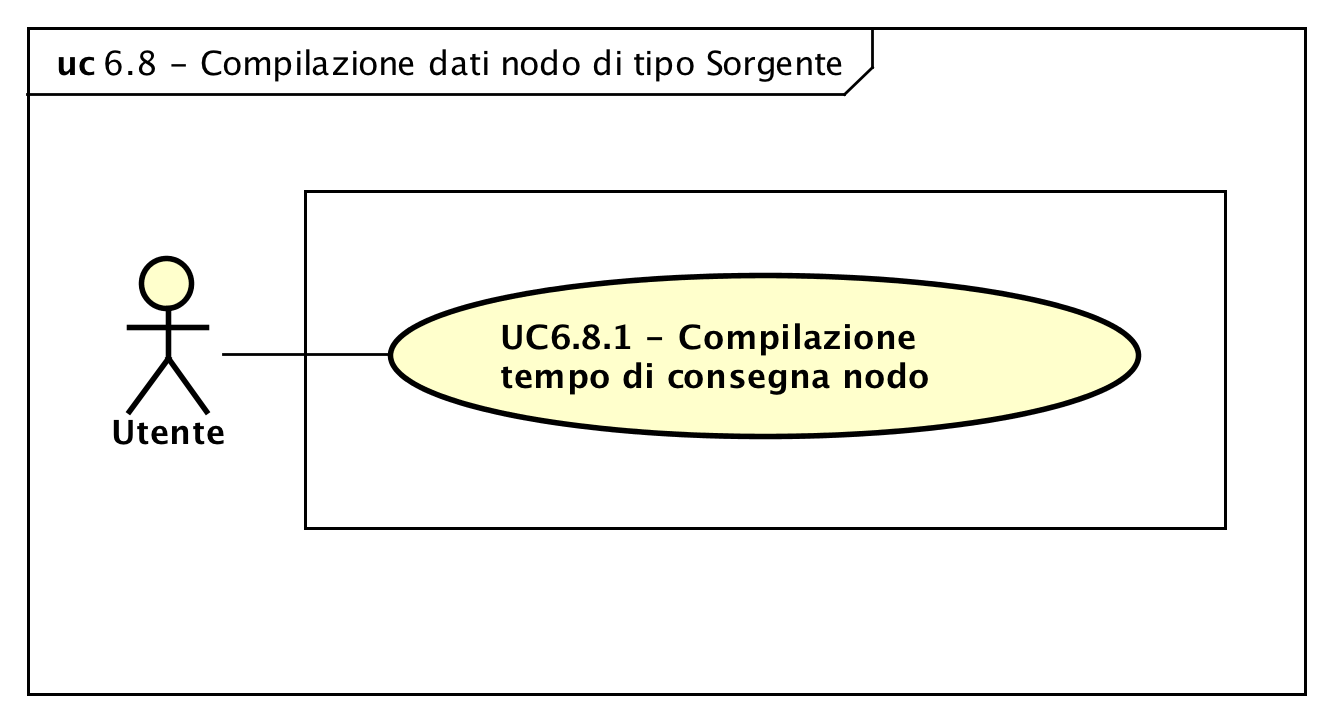
\includegraphics[scale=0.5]{{img/uc6.8}.png} 
	\caption{UC6.8 - Compilazione dati nodo di tipo Sorgente}
\end{figure}
\def\arraystretch{1.5}
\rowcolors{2}{D}{P}
\begin{tabularx}{\textwidth}{l|p{0.7\textwidth}}
	\rowcolor{I} \multicolumn{2}{c}{\color{white}\textbf{UC6.8 - Compilazione dati nodo di tipo Sorgente}} \\
	\toprule
	\endhead
	\textbf{Attori} & Utente\\
	\textbf{Descrizione} & l'utente compila i dati del nodo di tipo Sorgente\\
	\textbf{Pre-condizione} & l'utente ha posizionato il nodo; l'utente ha scelto come tipologia di nodo Sorgente\\
	\textbf{Post-condizione} & i dati del nodo di tipo Sorgente sono stati compilati; l'utente visualizza i dati appena compilati nell'area informativa\\
	\textbf{Scenario principale} & \vspace{-1.2em}\begin{enumerate}[leftmargin=*,noitemsep,nosep]
		\item \nameref{sssec:UC6.8.1}.
	\end{enumerate}\\
	%\textbf{Generalizzazioni} &  \\
	\bottomrule
\end{tabularx}
\subsection{UC6.8.1 - Compilazione tempo di consegna nodo} 
\label{sssec:UC6.8.1} 
\def\arraystretch{1.5}
\rowcolors{2}{D}{P}
\begin{tabularx}{\textwidth}{l|p{0.7\textwidth}}
	\rowcolor{I} \multicolumn{2}{c}{\color{white}\textbf{UC6.8.1 - Compilazione tempo di consegna nodo}} \\
	\toprule
	\endhead
	\textbf{Attori} & Utente\\
	\textbf{Descrizione} & l'utente compila il tempo di consegna del nodo\\
	\textbf{Pre-condizione} & il sistema offre la possibilità di compilare il tempo di consegna del nodo; l'utente ha scelto come tipologia di nodo Sorgente\\
	\textbf{Post-condizione} & l'utente ha compilato il tempo di consegna del nodo e visualizza il tempo appena compilato nell'area informativa\\
	\textbf{Scenario principale} & \vspace{-1.2em}\begin{enumerate}[leftmargin=*,noitemsep,nosep]
		\item \nameref{sssec:UC6.8.1}.
	\end{enumerate}\\
	%\textbf{Generalizzazioni} &  \\
	\bottomrule
\end{tabularx}
\subsection{UC6.9 - Compilazione dati nodo di tipo Risorsa} 
\label{sssec:UC6.9} 
\def\arraystretch{1.5}
\rowcolors{2}{D}{P}
\begin{tabularx}{\textwidth}{l|p{0.7\textwidth}}
	\rowcolor{I} \multicolumn{2}{c}{\color{white}\textbf{UC6.9 - Compilazione dati nodo di tipo Risorsa}} \\
	\toprule
	\endhead
	\textbf{Attori} & Utente\\
	\textbf{Descrizione} & l'utente compila i dati del nodo di tipo Risorsa\\
	\textbf{Pre-condizione} & l'utente ha posizionato il nodo; l'utente ha scelto come tipologia di nodo Risorsa\\
	\textbf{Post-condizione} & i dati del nodo di tipo Risorsa sono stati compilati; l'utente visualizza i dati appena compilati nell'area informativa\\
	\textbf{Scenario principale} & \vspace{-1.2em}\begin{enumerate}[leftmargin=*,noitemsep,nosep]
		\item \nameref{sssec:UC6.9}.
	\end{enumerate}\\
	%\textbf{Generalizzazioni} &  \\
	\bottomrule
\end{tabularx}
\subsection{UC6.10 - Conferma aggiunta nodo} 
\label{sssec:UC6.10} 
\def\arraystretch{1.5}
\rowcolors{2}{D}{P}
\begin{tabularx}{\textwidth}{l|p{0.7\textwidth}}
	\rowcolor{I} \multicolumn{2}{c}{\color{white}\textbf{UC6.10 - Conferma aggiunta nodo}} \\
	\toprule
	\endhead
	\textbf{Attori} & Utente\\
	\textbf{Descrizione} & l'utente conferma l'aggiunta di un nodo\\
	\textbf{Pre-condizione} & il sistema offre la possibilità di confermare l'aggiunta di un nodo\\
	\textbf{Post-condizione} & un nuovo nodo è stato aggiunto ed è visualizzabile sulla mappa; l'utente visualizza un messaggio che comunica la corretta esecuzione dell'operazione; l'area informativa rimane impostata sul nodo appena inserito; la posizione e il livello di ingrandimento della mappa rimangono invariati\\
	\textbf{Scenario principale} & \vspace{-1.2em}\begin{enumerate}[leftmargin=*,noitemsep,nosep]
		\item \nameref{sssec:UC6.10}.
	\end{enumerate}\\
	\textbf{Estensioni} & \vspace{-1.2em}\begin{itemize}[leftmargin=*,noitemsep,nosep]
		\item \nameref{sssec:UC6.11}: dati inseriti non validi:
		\begin{itemize}
			\item classe non scelta;
			\item nome vuoto; più lungo di 50 caratteri; inizia e/o finisce con uno spazio; contiene caratteri speciali;
			\item capacità vuota; più lunga di 5
			cifre per la parte intera; più di 2 per la parte decimale;
			\item tempo di processo vuoto; più lungo di 5 cifre per la parte intera; più di 2 per la parte decimale.
			\item valore (monetario) vuoto; più lungo di 20 cifre per la parte intera; più di 2 per la parte decimale;
			\item tempo di consegna vuoto; più lungo di 5 cifre per la parte intera; più di 2 per la parte decimale.
		\end{itemize}
	\end{itemize}\\
	%\textbf{Generalizzazioni} &  \\
	\bottomrule
\end{tabularx}
\subsection{UC6.11 - Visualizzazione errore aggiunta nodo} 
\label{sssec:UC6.11} 
\def\arraystretch{1.5}
\rowcolors{2}{D}{P}
\begin{tabularx}{\textwidth}{l|p{0.7\textwidth}}
	\rowcolor{I} \multicolumn{2}{c}{\color{white}\textbf{UC6.11 - Visualizzazione errore aggiunta nodo}} \\
	\toprule
	\endhead
	\textbf{Attori} & Utente\\
	\textbf{Descrizione} & l'utente visualizza un errore relativo ai dati del nodo compilati in modo errato\\
	\textbf{Pre-condizione} & l'utente sta tentando di inserire un nuovo nodo\\
	\textbf{Post-condizione} & nessun nuovo nodo aggiunto; l'utente visualizza un errore relativo ai dati del nodo compilati in modo errato; l'utente viene riportato alla schermata di aggiunta nodo\\
	\textbf{Scenario principale} & \vspace{-1.2em}\begin{enumerate}[leftmargin=*,noitemsep,nosep]
		\item \nameref{sssec:UC6.11}.
	\end{enumerate}\\
	%\textbf{Generalizzazioni} &  \\
	\bottomrule
\end{tabularx}
\subsection{UC7 - Visualizzazione info nodo} 
\label{sssec:UC7} 
\def\arraystretch{1.5}
\rowcolors{2}{D}{P}
\begin{tabularx}{\textwidth}{l|p{0.7\textwidth}}
	\rowcolor{I} \multicolumn{2}{c}{\color{white}\textbf{UC7 - Visualizzazione info nodo}} \\
	\toprule
	\endhead
	\textbf{Attori} & Utente\\
	\textbf{Descrizione} & l'utente seleziona un nodo e ne visualizza le informazioni\\
	\textbf{Pre-condizione} & l'utente ha aperto l'applicazione; è stato inserito almeno un nodo\\
	\textbf{Post-condizione} & il sistema mostra nell'area informativa le informazioni del nodo selezionato; la posizione e il livello di ingrandimento della mappa rimangono invariati\\
	\textbf{Scenario principale} & \vspace{-1.2em}\begin{enumerate}[leftmargin=*,noitemsep,nosep]
		\item \nameref{sssec:UC7}.
	\end{enumerate}\\
	%\textbf{Generalizzazioni} &  \\
	\bottomrule
\end{tabularx}
\subsection{UC8 - Chiusura visualizzazione info nodo} 
\label{sssec:UC8} 
\def\arraystretch{1.5}
\rowcolors{2}{D}{P}
\begin{tabularx}{\textwidth}{l|p{0.7\textwidth}}
	\rowcolor{I} \multicolumn{2}{c}{\color{white}\textbf{UC8 - Chiusura visualizzazione info nodo}} \\
	\toprule
	\endhead
	\textbf{Attori} & Utente\\
	\textbf{Descrizione} & l'utente chiude la visualizzazione delle informazioni di un nodo\\
	\textbf{Pre-condizione} & l'utente ha visualizzato le informazioni di un nodo\\
	\textbf{Post-condizione} & è stata chiusa la visualizzazione delle informazioni del nodo selezionato nell'area informativa; l'area informativa viene impostata sulla visualizzazione di default; la posizione e il livello di ingrandimento della mappa rimangono invariati\\
	\textbf{Scenario principale} & \vspace{-1.2em}\begin{enumerate}[leftmargin=*,noitemsep,nosep]
		\item \nameref{sssec:UC8}.
	\end{enumerate}\\
	%\textbf{Generalizzazioni} &  \\
	\bottomrule
\end{tabularx}
\subsection{UC9 - Modifica nodo} 
\label{sssec:UC9} 
\begin{figure}[H] 
	\centering 
	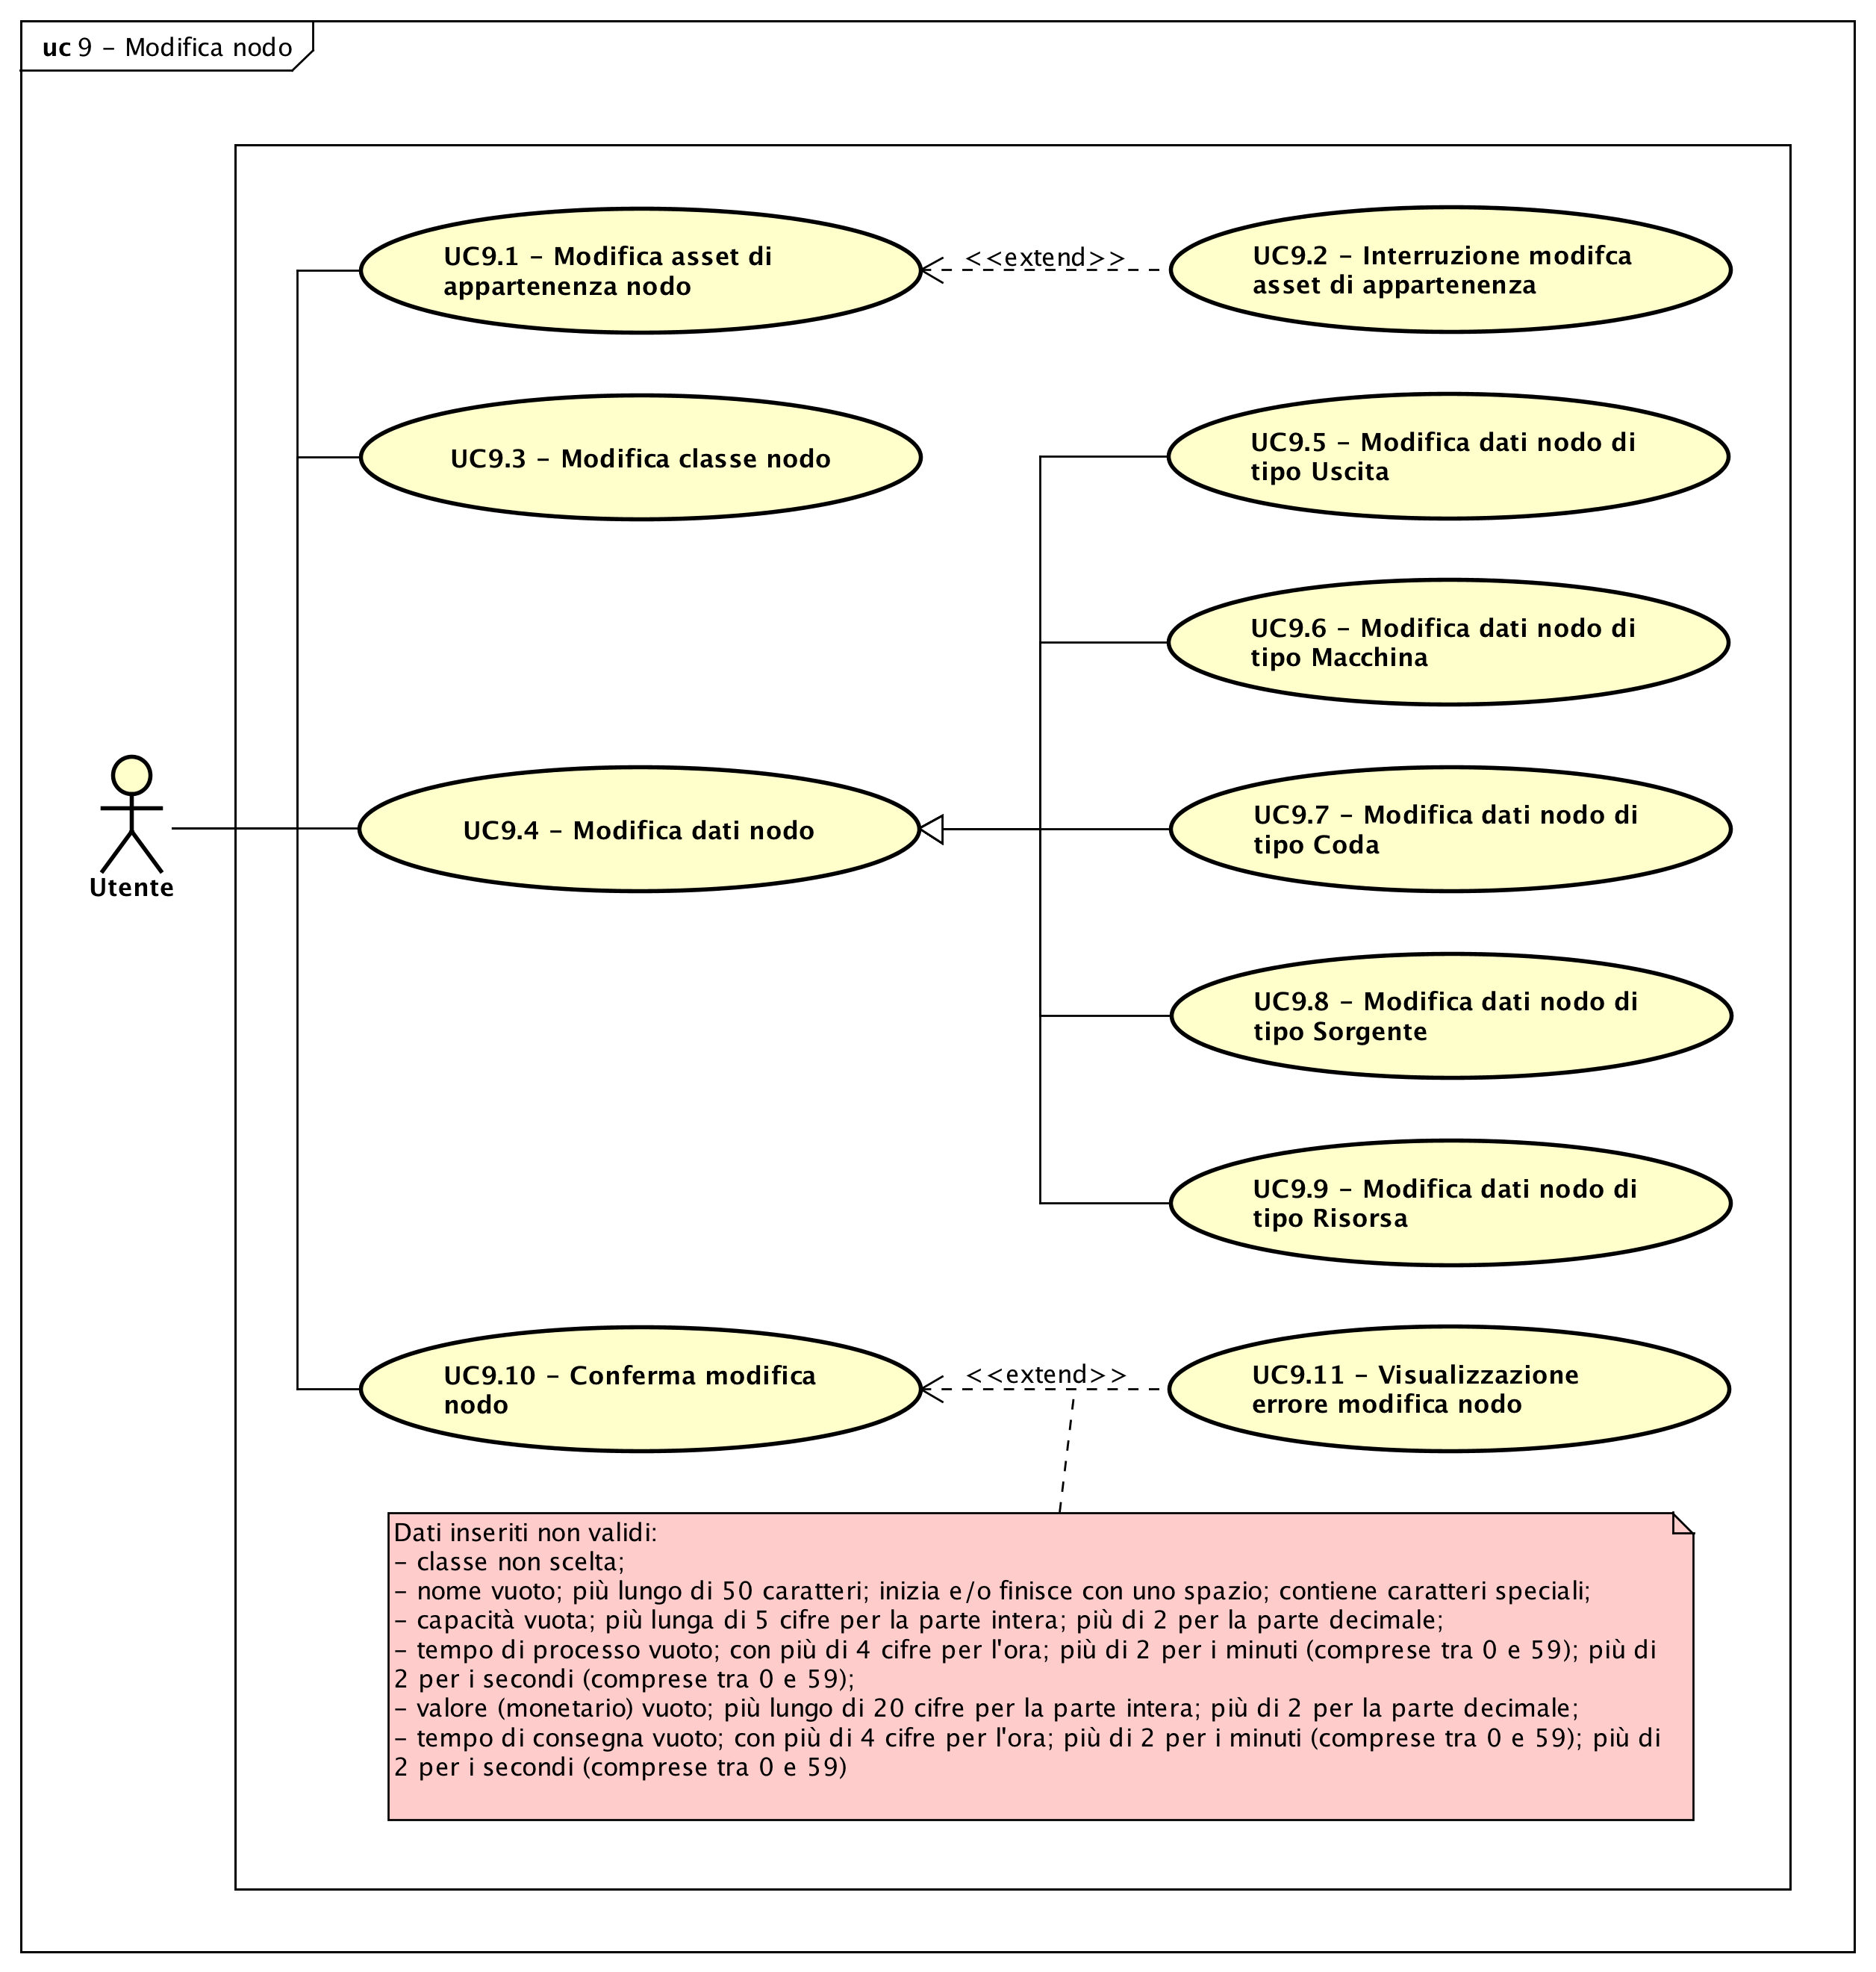
\includegraphics[width=\textwidth]{{img/uc9}.png} 
	\caption{UC9 - Modifica nodo}
\end{figure}
\def\arraystretch{1.5}
\rowcolors{2}{D}{P}
\begin{tabularx}{\textwidth}{l|p{0.7\textwidth}}
	\rowcolor{I} \multicolumn{2}{c}{\color{white}\textbf{UC9 - Modifica nodo}} \\
	\toprule
	\endhead
	\textbf{Attori} & Utente\\
	\textbf{Descrizione} & l'utente modifica il nodo\\
	\textbf{Pre-condizione} & l'utente ha aperto l'applicazione; almeno un nodo è stato aggiunto; l'utente ha selezionato un nodo\\
	\textbf{Post-condizione} & il nodo è stato modificato; l'utente visualizza un messaggio che comunica la corretta esecuzione dell'operazione; l'area informativa rimane impostata sul nodo appena modificato; la posizione e il livello di ingrandimento della mappa rimangono invariati\\
	\textbf{Scenario principale} & \vspace{-1.2em}\begin{enumerate}[leftmargin=*,noitemsep,nosep]
		\item \nameref{sssec:UC9.1};
		\item \nameref{sssec:UC9.2};
		\item \nameref{sssec:UC9.3};
		\item \nameref{sssec:UC9.4};
		\item \nameref{sssec:UC9.5} oppure
		\item \nameref{sssec:UC9.6} oppure
		\item \nameref{sssec:UC9.7} oppure
		\item \nameref{sssec:UC9.8} oppure
		\item \nameref{sssec:UC9.9};
		\item \nameref{sssec:UC9.10}.
	\end{enumerate}\\
	\textbf{Estensioni} & \vspace{-1.2em}\begin{itemize}[leftmargin=*,noitemsep,nosep]
		\item \nameref{sssec:UC34}.
	\end{itemize}\\
	\textbf{Scenari alternativi} & \vspace{-1.2em}\begin{itemize}[leftmargin=*,noitemsep,nosep]
		\item \nameref{sssec:UC9.11}.
	\end{itemize}\\
	%\textbf{Generalizzazioni} &  \\
	\bottomrule
\end{tabularx}
\subsection{UC9.1 - Modifica asset di appartenenza nodo} 
\label{sssec:UC9.1} 
\begin{figure}[H] 
	\centering 
	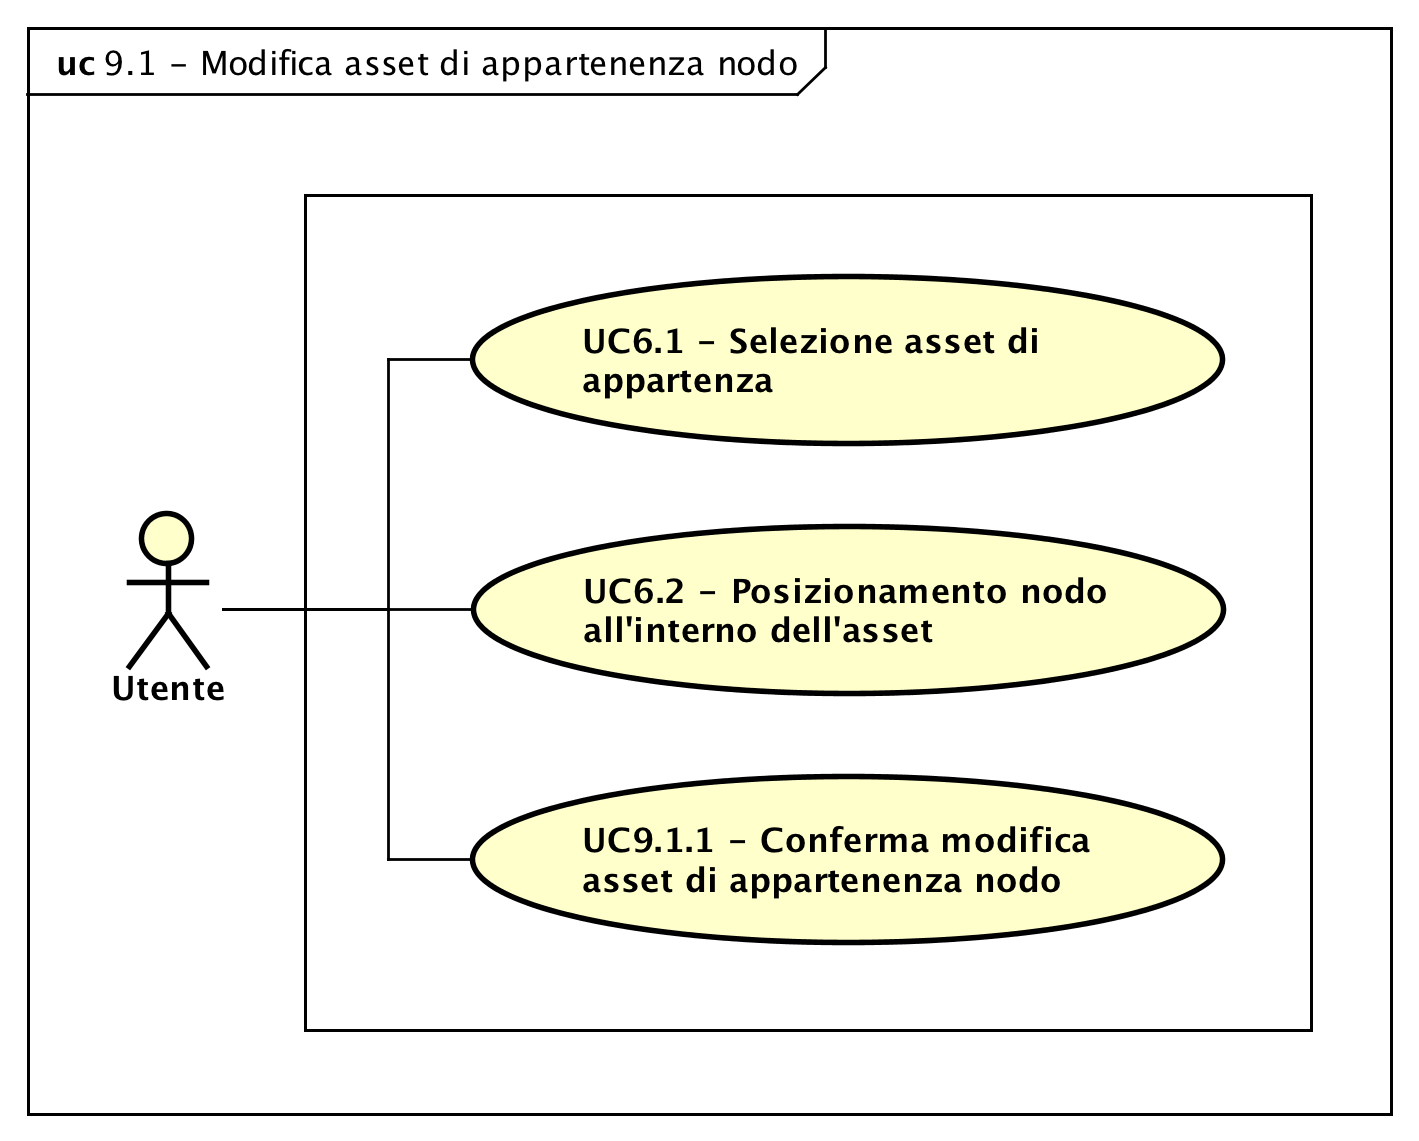
\includegraphics[scale=0.5]{{img/uc9.1}.png} 
	\caption{UC9.1 - Modifica asset di appartenenza nodo}
\end{figure}
\def\arraystretch{1.5}
\rowcolors{2}{D}{P}
\begin{tabularx}{\textwidth}{l|p{0.7\textwidth}}
	\rowcolor{I} \multicolumn{2}{c}{\color{white}\textbf{UC9.1 - Modifica asset di appartenenza nodo}} \\
	\toprule
	\endhead
	\textbf{Attori} & Utente\\
	\textbf{Descrizione} & l'utente modifica l'asset di appartenenza del nodo\\
	\textbf{Pre-condizione} & il sistema offre la possibilità di modificare l'asset di appartenenza del nodo\\
	\textbf{Post-condizione} & l'asset di appartenenza del nodo è stato modificato; il nodo viene spostato dal vecchio asset al nuovo ed è visualizzabile sulla mappa; l'utente può continuare a modificare altri dati del nodo\\
	\textbf{Scenario principale} & \vspace{-1.2em}\begin{enumerate}[leftmargin=*,noitemsep,nosep]
		\item \nameref{sssec:UC6.1}
		\item \nameref{sssec:UC6.2};
		\item \nameref{sssec:UC9.1.1}.
	\end{enumerate}\\
	\textbf{Estensioni} & \vspace{-1.2em}\begin{itemize}[leftmargin=*,noitemsep,nosep]
		\item \nameref{sssec:UC9.2}: l'utente interrompe volontariamente la modifica dell'asset di appartenenza del nodo
	\end{itemize}\\
	%\textbf{Generalizzazioni} &  \\
	\bottomrule
\end{tabularx}
\subsection{UC9.1.1 - Conferma modifica asset di appartenenza nodo} 
\label{sssec:UC9.1.1} 
\def\arraystretch{1.5}
\rowcolors{2}{D}{P}
\begin{tabularx}{\textwidth}{l|p{0.7\textwidth}}
	\rowcolor{I} \multicolumn{2}{c}{\color{white}\textbf{UC9.1.1 - Conferma modifica asset di appartenenza nodo}} \\
	\toprule
	\endhead
	\textbf{Attori} & Utente\\
	\textbf{Descrizione} & l'utente conferma la modifica dell'asset di appartenenza del nodo\\
	\textbf{Pre-condizione} & il sistema offre la possibilità di confermare l'asset di appartenenza del nodo\\
	\textbf{Post-condizione} & l'asset di appartenenza del nodo è stato modificato; il nodo viene spostato dall'asset che lo conteneva precedentemente al nuovo asset di appartenenza; l'utente può continuare a modificare altri dati del nodo\\
	\textbf{Scenario principale} & \vspace{-1.2em}\begin{enumerate}[leftmargin=*,noitemsep,nosep]
		\item \nameref{sssec:UC9.1.1}.
	\end{enumerate}\\
	%\textbf{Generalizzazioni} &  \\
	\bottomrule
\end{tabularx}

\subsection{UC9.2 - Interruzione modifica asset di appartenenza} 
\label{sssec:UC9.2} 
\def\arraystretch{1.5}
\rowcolors{2}{D}{P}
\begin{tabularx}{\textwidth}{l|p{0.7\textwidth}}
	\rowcolor{I} \multicolumn{2}{c}{\color{white}\textbf{UC9.2 - Interruzione modifica asset di appartenenza}} \\
	\toprule
	\endhead
	\textbf{Attori} & Utente\\
	\textbf{Descrizione} & l'utente interrompe la modifica dell'asset di appartenenza del nodo\\
	\textbf{Pre-condizione} & il sistema offre la possibilità di modificare l'asset di appartenenza\\
	\textbf{Post-condizione} & l'asset di appartenenza del nodo non è stato modificato; l'utente viene riportato alla schermata di modifica nodo e può modificarne altri dati\\
	\textbf{Scenario principale} & \vspace{-1.2em}\begin{enumerate}[leftmargin=*,noitemsep,nosep]
		\item \nameref{sssec:UC9.2}.
	\end{enumerate}\\
	%\textbf{Generalizzazioni} &  \\
	\bottomrule
\end{tabularx}
\subsection{UC9.3 - Modifica classe nodo} 
\label{sssec:UC9.3} 
\def\arraystretch{1.5}
\rowcolors{2}{D}{P}
\begin{tabularx}{\textwidth}{l|p{0.7\textwidth}}
	\rowcolor{I} \multicolumn{2}{c}{\color{white}\textbf{UC9.3 - Modifica classe nodo}} \\
	\toprule
	\endhead
	\textbf{Attori} & Utente\\
	\textbf{Descrizione} & l'utente modifica la classe del nodo\\
	\textbf{Pre-condizione} & il sistema offre la possibilità di modificare la classe del nodo\\
	\textbf{Post-condizione} & la classe del nodo è stata modificata; la forma del nodo sulla mappa cambia in base alla classe scelta\\
	\textbf{Scenario principale} & \vspace{-1.2em}\begin{enumerate}[leftmargin=*,noitemsep,nosep]
		\item \nameref{sssec:UC9.2}.
	\end{enumerate}\\
	%\textbf{Generalizzazioni} &  \\
	\bottomrule
\end{tabularx}
\subsection{UC9.4 - Modifica dati nodo} 
\label{sssec:UC9.4} 
\begin{figure}[H] 
	\centering 
	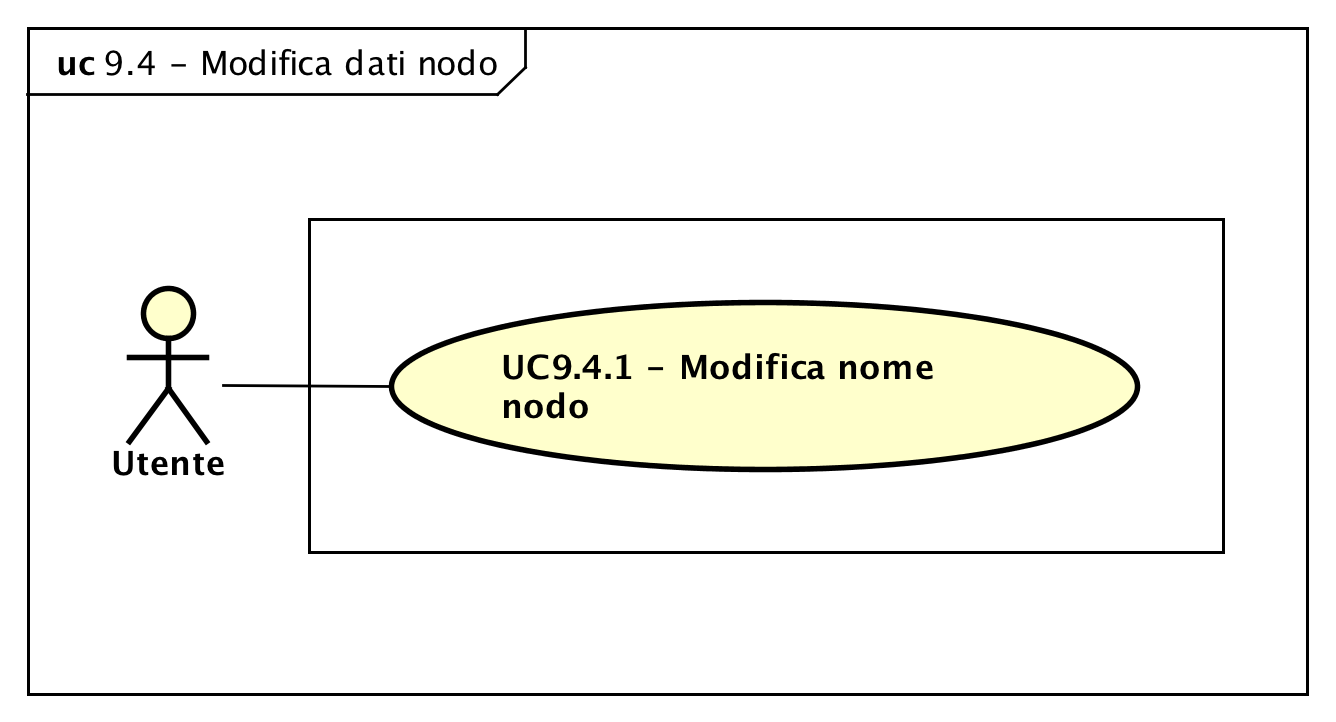
\includegraphics[scale=0.5]{{img/uc9.4}.png} 
	\caption{UC9.4 - Modifica dati nodo}
\end{figure}
\def\arraystretch{1.5}
\rowcolors{2}{D}{P}
\begin{tabularx}{\textwidth}{l|p{0.7\textwidth}}
	\rowcolor{I} \multicolumn{2}{c}{\color{white}\textbf{UC9.4 - Modifica dati nodo}} \\
	\toprule
	\endhead
	\textbf{Attori} & Utente\\
	\textbf{Descrizione} & l'utente modifica i dati del nodo\\
	\textbf{Pre-condizione} & il sistema offre la possibilità di modificare i dati del nodo;\\
	\textbf{Post-condizione} & i dati del nodo sono stati modificati; l'utente visualizza i dati appena modificati nell'area informativa\\
	\textbf{Scenario principale} & \vspace{-1.2em}\begin{enumerate}[leftmargin=*,noitemsep,nosep]
		\item \nameref{sssec:UC9.4.1}.
	\end{enumerate}\\
	\textbf{Generalizzazioni} &
	\vspace{-1.2em}\begin{itemize}
		[leftmargin=*,noitemsep,nosep]
		\item \nameref{sssec:UC9.5};
		\item \nameref{sssec:UC9.6};
		\item \nameref{sssec:UC9.7};
		\item \nameref{sssec:UC9.8};
		\item \nameref{sssec:UC9.9}.
	\end{itemize} \\
	\bottomrule
\end{tabularx}
\subsection{UC9.4.1 - Modifica nome nodo} 
\label{sssec:UC9.4.1} 
\def\arraystretch{1.5}
\rowcolors{2}{D}{P}
\begin{tabularx}{\textwidth}{l|p{0.7\textwidth}}
	\rowcolor{I} \multicolumn{2}{c}{\color{white}\textbf{UC9.4.1 - Modifica nome nodo}} \\
	\toprule
	\endhead
	\textbf{Attori} & Utente\\
	\textbf{Descrizione} & l'utente modifica il campo relativo al nome del nodo\\
	\textbf{Pre-condizione} & il sistema offre la possibilità di modificare il nome del nodo\\
	\textbf{Post-condizione} & il campo relativo al nome del nodo è stato modificato; l'utente visualizza il nome appena modificato nell'area informativa\\
	\textbf{Scenario principale} & \vspace{-1.2em}\begin{enumerate}[leftmargin=*,noitemsep,nosep]
		\item \nameref{sssec:UC9.4.1}.
	\end{enumerate}\\
	%\textbf{Generalizzazioni} &  \\
	\bottomrule
\end{tabularx}
\subsection{UC9.5 - Modifica dati nodo di tipo Uscita} 
\label{sssec:UC9.5} 
\def\arraystretch{1.5}
\rowcolors{2}{D}{P}
\begin{tabularx}{\textwidth}{l|p{0.7\textwidth}}
	\rowcolor{I} \multicolumn{2}{c}{\color{white}\textbf{UC9.5 - Modifica dati nodo di tipo Uscita}} \\
	\toprule
	\endhead
	\textbf{Attori} & Utente\\
	\textbf{Descrizione} & l'utente modifica i dati del nodo di tipo Uscita\\
	\textbf{Pre-condizione} & il sistema offre la possibilità di modificare i dati del nodo; l'utente ha scelto un nodo di tipo Uscita\\
	\textbf{Post-condizione} & i dati del nodo sono stati modificati; l'utente visualizza i dati appena modificati nell'area informativa\\
	\textbf{Scenario principale} & \vspace{-1.2em}\begin{enumerate}[leftmargin=*,noitemsep,nosep]
		\item \nameref{sssec:UC9.5}.
	\end{enumerate}\\
	%\textbf{Generalizzazioni} &  \\
	\bottomrule
\end{tabularx}
\subsection{UC9.6 - Modifica dati nodo di tipo Macchina} 
\label{sssec:UC9.6} 
\begin{figure}[H] 
	\centering 
	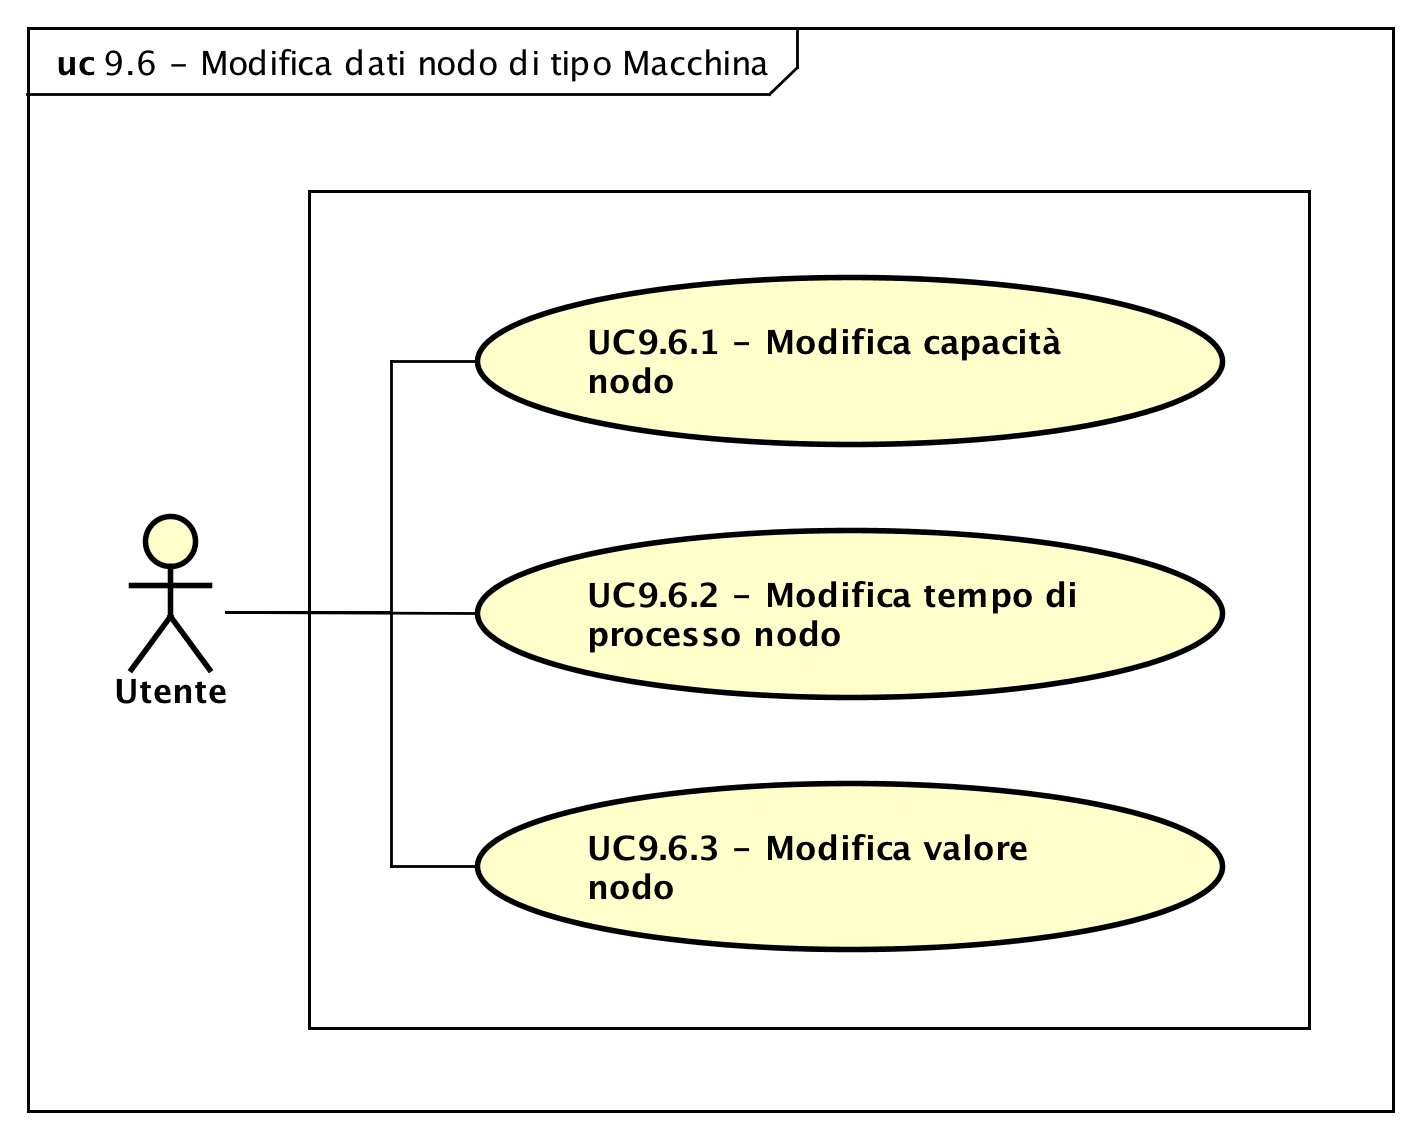
\includegraphics[scale=0.5]{{img/uc9.6}.png} 
	\caption{UC9.6 - Modifica dati nodo di tipo Macchina}
\end{figure}
\def\arraystretch{1.5}
\rowcolors{2}{D}{P}
\begin{tabularx}{\textwidth}{l|p{0.7\textwidth}}
	\rowcolor{I} \multicolumn{2}{c}{\color{white}\textbf{UC9.6 - Modifica dati nodo di tipo Macchina}} \\
	\toprule
	\endhead
	\textbf{Attori} & Utente\\
	\textbf{Descrizione} & l'utente modifica i dati del nodo di tipo Macchina\\
	\textbf{Pre-condizione} & il sistema offre la possibilità di modificare i dati del nodo; l'utente ha scelto un nodo di tipo Macchina\\
	\textbf{Post-condizione} & i dati del nodo sono stati modificati; l'utente visualizza i dati appena modificati nell'area informativa\\
	\textbf{Scenario principale} & \vspace{-1.2em}\begin{enumerate}[leftmargin=*,noitemsep,nosep]
		\item \nameref{sssec:UC9.6.1};
		\item \nameref{sssec:UC9.6.2};
		\item \nameref{sssec:UC9.6.3}.
	\end{enumerate}\\
	%\textbf{Generalizzazioni} &  \\
	\bottomrule
\end{tabularx}
\subsection{UC9.6.1 - Modifica capacità nodo} 
\label{sssec:UC9.6.1} 
\def\arraystretch{1.5}
\rowcolors{2}{D}{P}
\begin{tabularx}{\textwidth}{l|p{0.7\textwidth}}
	\rowcolor{I} \multicolumn{2}{c}{\color{white}\textbf{UC9.6.1 - Modifica capacità nodo}} \\
	\toprule
	\endhead
	\textbf{Attori} & Utente\\
	\textbf{Descrizione} & l'utente modifica il campo relativo alla capacità del nodo\\
	\textbf{Pre-condizione} & il sistema offre la possibilità di modificare la capacità del nodo; l'utente ha scelto come classe del nodo Macchina o Coda\\
	\textbf{Post-condizione} & il campo relativo alla capacità del nodo è stato modificato; l'utente visualizza la capacità del nodo appena modificata\\
	\textbf{Scenario principale} & \vspace{-1.2em}\begin{enumerate}[leftmargin=*,noitemsep,nosep]
		\item \nameref{sssec:UC9.6.1}.
	\end{enumerate}\\
	%\textbf{Generalizzazioni} &  \\
	\bottomrule
\end{tabularx}
\subsection{UC9.6.2 - Modifica tempo di processo nodo} 
\label{sssec:UC9.6.2} 
\def\arraystretch{1.5}
\rowcolors{2}{D}{P}
\begin{tabularx}{\textwidth}{l|p{0.7\textwidth}}
	\rowcolor{I} \multicolumn{2}{c}{\color{white}\textbf{UC9.6.2 - Modifica tempo di processo nodo}} \\
	\toprule
	\endhead
	\textbf{Attori} & Utente\\
	\textbf{Descrizione} & l'utente modifica il campo relativo al tempo di processo del nodo\\
	\textbf{Pre-condizione} & il sistema offre la possibilità di modificare il tempo di processo del nodo; l'utente ha scelto come classe del nodo Macchina\\
	\textbf{Post-condizione} & il campo relativo al tempo di processo del nodo è stato modificato; l'utente visualizza il tempo di processo appena modificato\\
	\textbf{Scenario principale} & \vspace{-1.2em}\begin{enumerate}[leftmargin=*,noitemsep,nosep]
		\item \nameref{sssec:UC9.6.2}.
	\end{enumerate}\\
	%\textbf{Generalizzazioni} &  \\
	\bottomrule
\end{tabularx}
\subsection{UC9.6.3 - Modifica valore nodo} 
\label{sssec:UC9.6.3} 
\def\arraystretch{1.5}
\rowcolors{2}{D}{P}
\begin{tabularx}{\textwidth}{l|p{0.7\textwidth}}
	\rowcolor{I} \multicolumn{2}{c}{\color{white}\textbf{UC9.6.3 - Modifica valore nodo}} \\
	\toprule
	\endhead
	\textbf{Attori} & Utente\\
	\textbf{Descrizione} & l'utente modifica il campo relativo al valore del nodo\\
	\textbf{Pre-condizione} & il sistema offre la possibilità di modificare il valore del nodo; l'utente ha scelto come classe del nodo Macchina\\
	\textbf{Post-condizione} & il campo relativo al valore del nodo è stato modificato; l'utente visualizza il valore appena modificato\\
	\textbf{Scenario principale} & \vspace{-1.2em}\begin{enumerate}[leftmargin=*,noitemsep,nosep]
		\item \nameref{sssec:UC9.6.3}.
	\end{enumerate}\\
	%\textbf{Generalizzazioni} &  \\
	\bottomrule
\end{tabularx}
\subsection{UC9.7 - Modifica dati nodo di tipo Coda} 
\label{sssec:UC9.7} 
\begin{figure}[H] 
	\centering 
	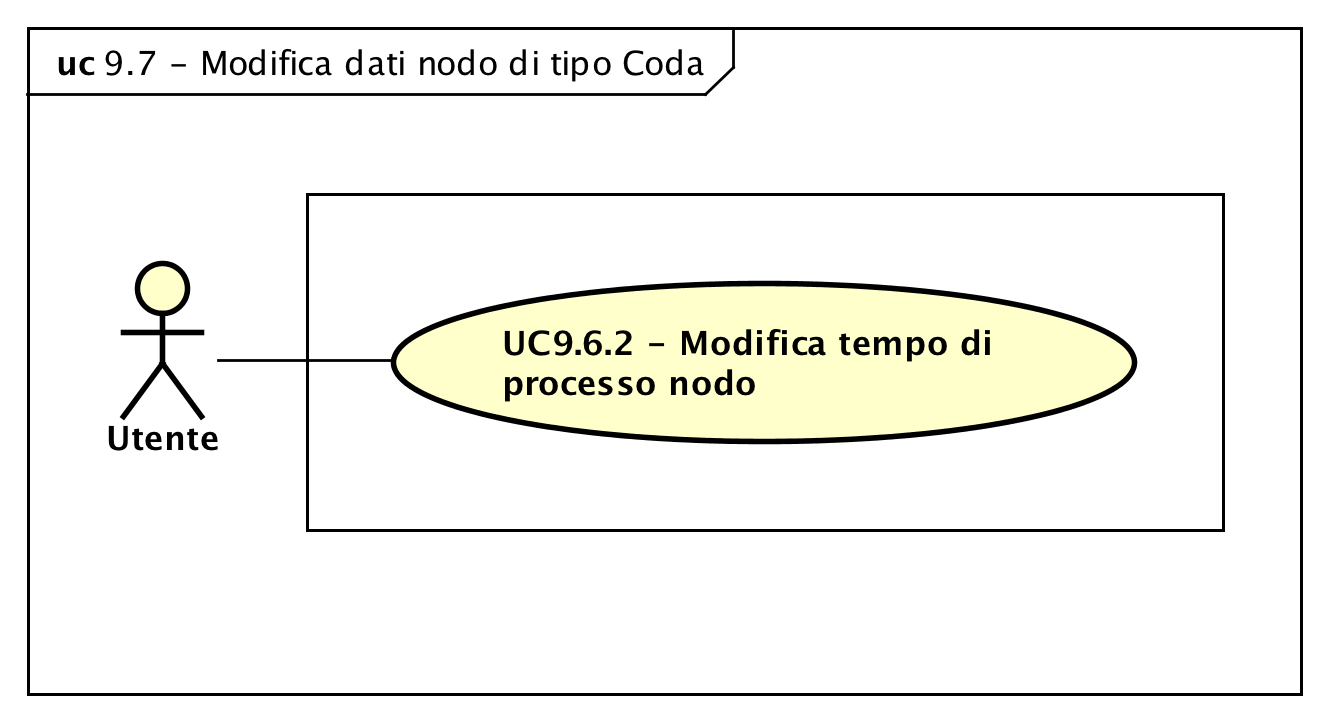
\includegraphics[scale=0.5]{{img/uc9.7}.png} 
	\caption{UC9.7 - Modifica dati nodo di tipo Coda}
\end{figure}
\def\arraystretch{1.5}
\rowcolors{2}{D}{P}
\begin{tabularx}{\textwidth}{l|p{0.7\textwidth}}
	\rowcolor{I} \multicolumn{2}{c}{\color{white}\textbf{UC9.7 - Modifica dati nodo di tipo Coda}} \\
	\toprule
	\endhead
	\textbf{Attori} & Utente\\
	\textbf{Descrizione} & l'utente modifica i dati del nodo di tipo Coda\\
	\textbf{Pre-condizione} & il sistema offre la possibilità di modificare i dati del nodo; l'utente ha scelto un nodo di tipo Coda\\
	\textbf{Post-condizione} & i dati del nodo sono stati modificati; l'utente visualizza i dati appena modificati nell'area informativa\\
	\textbf{Scenario principale} & \vspace{-1.2em}\begin{enumerate}[leftmargin=*,noitemsep,nosep]
		\item \nameref{sssec:UC9.6.2}.
	\end{enumerate}\\
	%\textbf{Generalizzazioni} &  \\
	\bottomrule
\end{tabularx}
\subsection{UC9.8 - Modifica dati nodo di tipo Sorgente} 
\label{sssec:UC9.8} 
\begin{figure}[H] 
	\centering 
	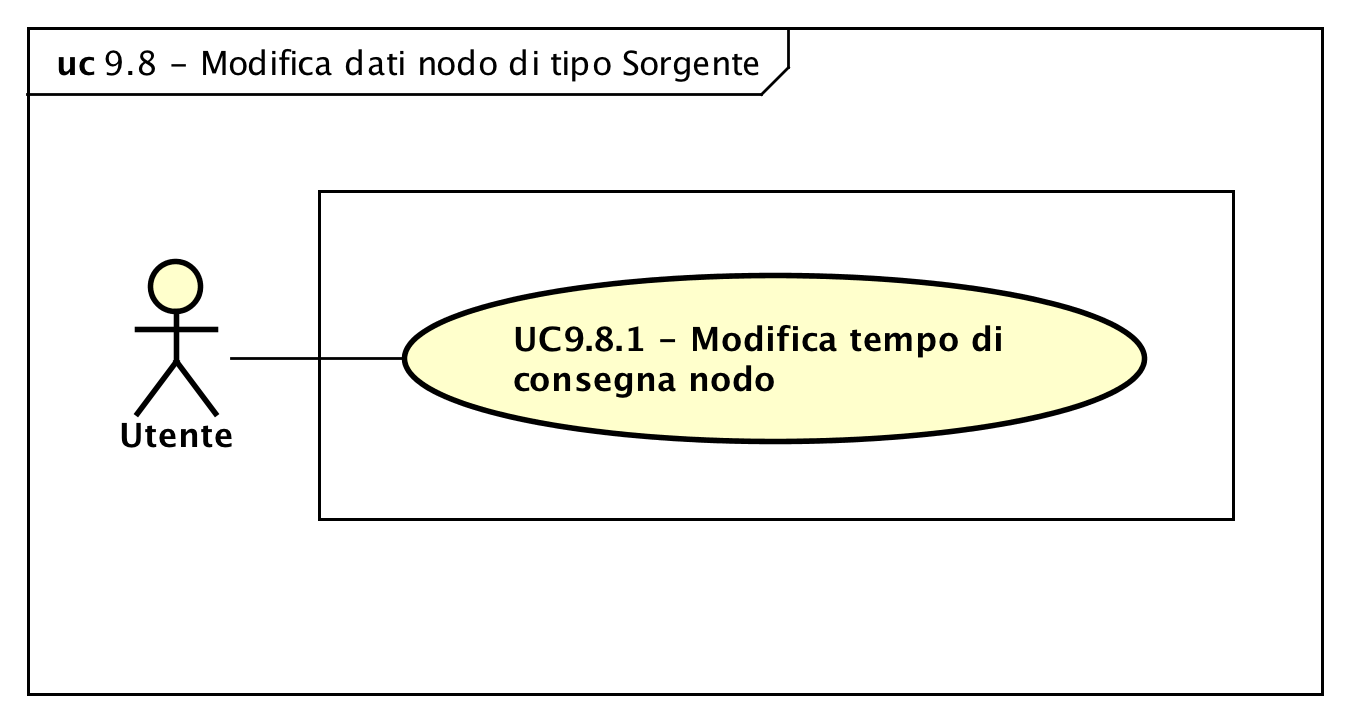
\includegraphics[scale=0.5]{{img/uc9.8}.png} 
	\caption{UC9.8 - Modifica dati nodo di tipo Sorgente}
\end{figure}
\def\arraystretch{1.5}
\rowcolors{2}{D}{P}
\begin{tabularx}{\textwidth}{l|p{0.7\textwidth}}
	\rowcolor{I} \multicolumn{2}{c}{\color{white}\textbf{UC9.8 - Modifica dati nodo di tipo Sorgente}} \\
	\toprule
	\endhead
	\textbf{Attori} & Utente\\
	\textbf{Descrizione} & l'utente modifica i dati del nodo di tipo Sorgente\\
	\textbf{Pre-condizione} & il sistema offre la possibilità di modificare i dati del nodo; l'utente ha scelto un nodo di tipo Sorgente\\
	\textbf{Post-condizione} & i dati del nodo sono stati modificati; l'utente visualizza i dati appena modificati nell'area informativa\\
	\textbf{Scenario principale} & \vspace{-1.2em}\begin{enumerate}[leftmargin=*,noitemsep,nosep]
		\item \nameref{sssec:UC9.8.1}.
	\end{enumerate}\\
	%\textbf{Generalizzazioni} &  \\
	\bottomrule
\end{tabularx}
\subsection{UC9.8.1 - Modifica tempo di consegna nodo} 
\label{sssec:UC9.8.1} 
\def\arraystretch{1.5}
\rowcolors{2}{D}{P}
\begin{tabularx}{\textwidth}{l|p{0.7\textwidth}}
	\rowcolor{I} \multicolumn{2}{c}{\color{white}\textbf{UC9.8.1 - Modifica tempo di consegna nodo}} \\
	\toprule
	\endhead
	\textbf{Attori} & Utente\\
	\textbf{Descrizione} & l'utente modifica il campo relativo al  tempo di consegna del nodo\\
	\textbf{Pre-condizione} & il sistema offre la possibilità di modificare il tempo di consegna del nodo; l'utente ha scelto come classe del nodo Sorgente\\
	\textbf{Post-condizione} & il campo relativo al tempo di consegna del nodo è stato modificato; l'utente visualizza il tempo di consegna appena modificato\\
	\textbf{Scenario principale} & \vspace{-1.2em}\begin{enumerate}[leftmargin=*,noitemsep,nosep]
		\item \nameref{sssec:UC9.8.1}.
	\end{enumerate}\\
	%\textbf{Generalizzazioni} &  \\
	\bottomrule
\end{tabularx}
\subsection{UC9.9 - Modifica dati nodo di tipo Risorsa} 
\label{sssec:UC9.9} 
\def\arraystretch{1.5}
\rowcolors{2}{D}{P}
\begin{tabularx}{\textwidth}{l|p{0.7\textwidth}}
	\rowcolor{I} \multicolumn{2}{c}{\color{white}\textbf{UC9.9 - Modifica dati nodo di tipo Risorsa}} \\
	\toprule
	\endhead
	\textbf{Attori} & Utente\\
	\textbf{Descrizione} & l'utente modifica i dati del nodo di tipo Risorsa\\
	\textbf{Pre-condizione} & il sistema offre la possibilità di modificare i dati del nodo; l'utente ha scelto un nodo di tipo Risorsa\\
	\textbf{Post-condizione} & i dati del nodo sono stati modificati; l'utente visualizza i dati appena modificati nell'area informativa\\
	\textbf{Scenario principale} & \vspace{-1.2em}\begin{enumerate}[leftmargin=*,noitemsep,nosep]
		\item \nameref{sssec:UC9.9}.
	\end{enumerate}\\
	%\textbf{Generalizzazioni} &  \\
	\bottomrule
\end{tabularx}
\subsection{UC9.10 - Conferma modifica nodo} 
\label{sssec:UC9.10} 
\def\arraystretch{1.5}
\rowcolors{2}{D}{P}
\begin{tabularx}{\textwidth}{l|p{0.7\textwidth}}
	\rowcolor{I} \multicolumn{2}{c}{\color{white}\textbf{UC9.10 - Conferma modifica nodo}} \\
	\toprule
	\endhead
	\textbf{Attori} & Utente\\
	\textbf{Descrizione} & l'utente conferma la modifica del nodo\\
	\textbf{Pre-condizione} & il sistema offre la possibilità di confermare la modifica del nodo\\
	\textbf{Post-condizione} & il nodo è stato modificato;  l'utente visualizza un messaggio che comunica la corretta esecuzione dell'operazione; l'area informativa rimane impostata sul nodo appena modificato; la posizione e il livello di ingrandimento della mappa rimangono invariati\\
	\textbf{Scenario principale} & \vspace{-1.2em}\begin{enumerate}[leftmargin=*,noitemsep,nosep]
		\item \nameref{sssec:UC9.10}.
	\end{enumerate}\\
	\textbf{Estensioni} & \vspace{-1.2em}\begin{itemize}[leftmargin=*,noitemsep,nosep]
		\item \nameref{sssec:UC9.11}: dati inseriti non validi:
		\begin{itemize}
			\item classe non scelta;
			\item nome vuoto; più lungo di 50
			caratteri; inizia e/o finisce con uno spazio; contiene caratteri
			speciali;
			\item capacità vuota; più lunga di 5
			cifre per la parte intera; più di 2 per la parte decimale;
			\item tempo di processo vuoto; più lungo di 5 cifre per la parte intera; più di 2 per la parte decimale.
			\item valore (monetario) vuoto; più
			lungo di 20 cifre per la parte intera; più di 2 per la parte
			decimale;
			\item tempo di consegna vuoto; più lungo di 5 cifre per la parte intera; più di 2 per la parte decimale.
		\end{itemize}
	\end{itemize}\\
	%\textbf{Generalizzazioni} &  \\
	\bottomrule
\end{tabularx}
\subsection{UC9.11 - Visualizzazione errore modifica nodo} 
\label{sssec:UC9.11} 
\def\arraystretch{1.5}
\rowcolors{2}{D}{P}
\begin{tabularx}{\textwidth}{l|p{0.7\textwidth}}
	\rowcolor{I} \multicolumn{2}{c}{\color{white}\textbf{UC9.11 - Visualizzazione errore modifica nodo}} \\
	\toprule
	\endhead
	\textbf{Attori} & Utente\\
	\textbf{Descrizione} & l'utente visualizza un errore relativo alla modifica del nodo\\
	\textbf{Pre-condizione} & l'utente ha confermato la modifica dei dati del nodo\\
	\textbf{Post-condizione} & il nodo non è stato modificato; l'utente visualizza un errore relativo ai dati del nodo compilati in modo errato; l'utente viene riportato alla schermata di modifica nodo\\
	\textbf{Scenario principale} & \vspace{-1.2em}\begin{enumerate}[leftmargin=*,noitemsep,nosep]
		\item \nameref{sssec:UC9.11}.
	\end{enumerate}\\
	%\textbf{Generalizzazioni} &  \\
	\bottomrule
\end{tabularx}
\subsection{UC10 - Eliminazione nodo} 
\label{sssec:UC10} 
\begin{figure}[H] 
	\centering 
	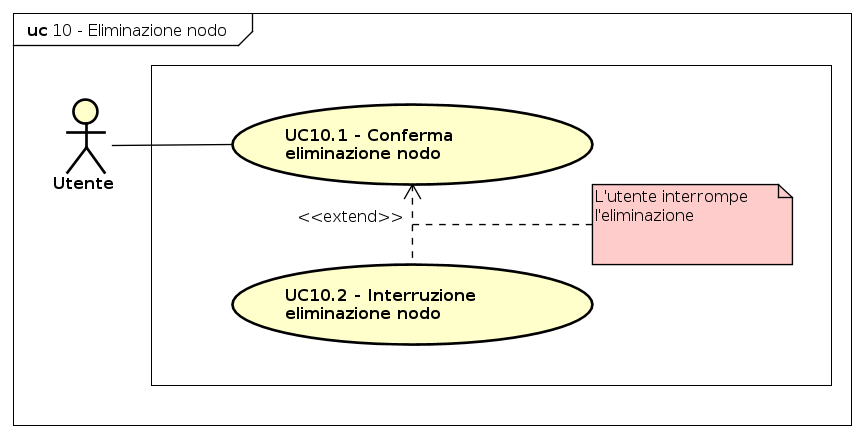
\includegraphics[scale=0.5]{{img/uc10}.png} 
	\caption{UC10 - Eliminazione nodo}
\end{figure}
\def\arraystretch{1.5}
\rowcolors{2}{D}{P}
\begin{tabularx}{\textwidth}{l|p{0.7\textwidth}}
	\rowcolor{I} \multicolumn{2}{c}{\color{white}\textbf{UC10 - Eliminazione nodo}} \\
	\toprule
	\endhead
	\textbf{Attori} & Utente\\
	\textbf{Descrizione} & l'utente elimina un nodo\\
	\textbf{Pre-condizione} & l'utente ha aperto l'applicazione; è stato inserito almeno un nodo; l'utente ha selezionato un nodo\\
	\textbf{Post-condizione} & il nodo è stato eliminato e non è più visibile sulla mappa; sono stati eliminati anche gli archi relativi a quel nodo; l'utente visualizza un messaggio che comunica la corretta esecuzione dell'operazione; l'area informativa viene impostata sulla visualizzazione di default;  la posizione e il livello di ingrandimento della mappa rimangono invariati\\
	\textbf{Scenario principale} & \vspace{-1.2em}\begin{enumerate}[leftmargin=*,noitemsep,nosep]
		\item \nameref{sssec:UC10.1}.
	\end{enumerate}\\
	\textbf{Estensioni} & \vspace{-1.2em}\begin{itemize}[leftmargin=*,noitemsep,nosep]
		\item \nameref{sssec:UC35}: l'utente interrompe volontariamente l'eliminazione del nodo
	\end{itemize}\\
	%\textbf{Generalizzazioni} &  \\
	\bottomrule
\end{tabularx}
\subsection{UC10.1 - Conferma eliminazione nodo} 
\label{sssec:UC10.1} 
\def\arraystretch{1.5}
\rowcolors{2}{D}{P}
\begin{tabularx}{\textwidth}{l|p{0.7\textwidth}}
	\rowcolor{I} \multicolumn{2}{c}{\color{white}\textbf{UC10.1 - Conferma eliminazione nodo}} \\
	\toprule
	\endhead
	\textbf{Attori} & Utente\\
	\textbf{Descrizione} & l'utente conferma l'eliminazione del nodo\\
	\textbf{Pre-condizione} & il sistema offre la possibilità di confermare l'eliminazione del nodo\\
	\textbf{Post-condizione} & il nodo è stato eliminato e non è più visibile sulla mappa; sono stati eliminati anche gli archi relativi a quel nodo; l'utente visualizza un messaggio che comunica la corretta esecuzione dell'operazione; l'area informativa viene impostata sulla visualizzazione di default;  la posizione e il livello di ingrandimento della mappa rimangono invariati\\
	\textbf{Scenario principale} & \vspace{-1.2em}\begin{enumerate}[leftmargin=*,noitemsep,nosep]
		\item \nameref{sssec:UC10.1}.
	\end{enumerate}\\
	%\textbf{Generalizzazioni} &  \\
	\bottomrule
\end{tabularx}
\subsection{UC11 - Aggiunta arco} 
\label{sssec:UC11} 
\begin{figure}[H] 
	\centering 
	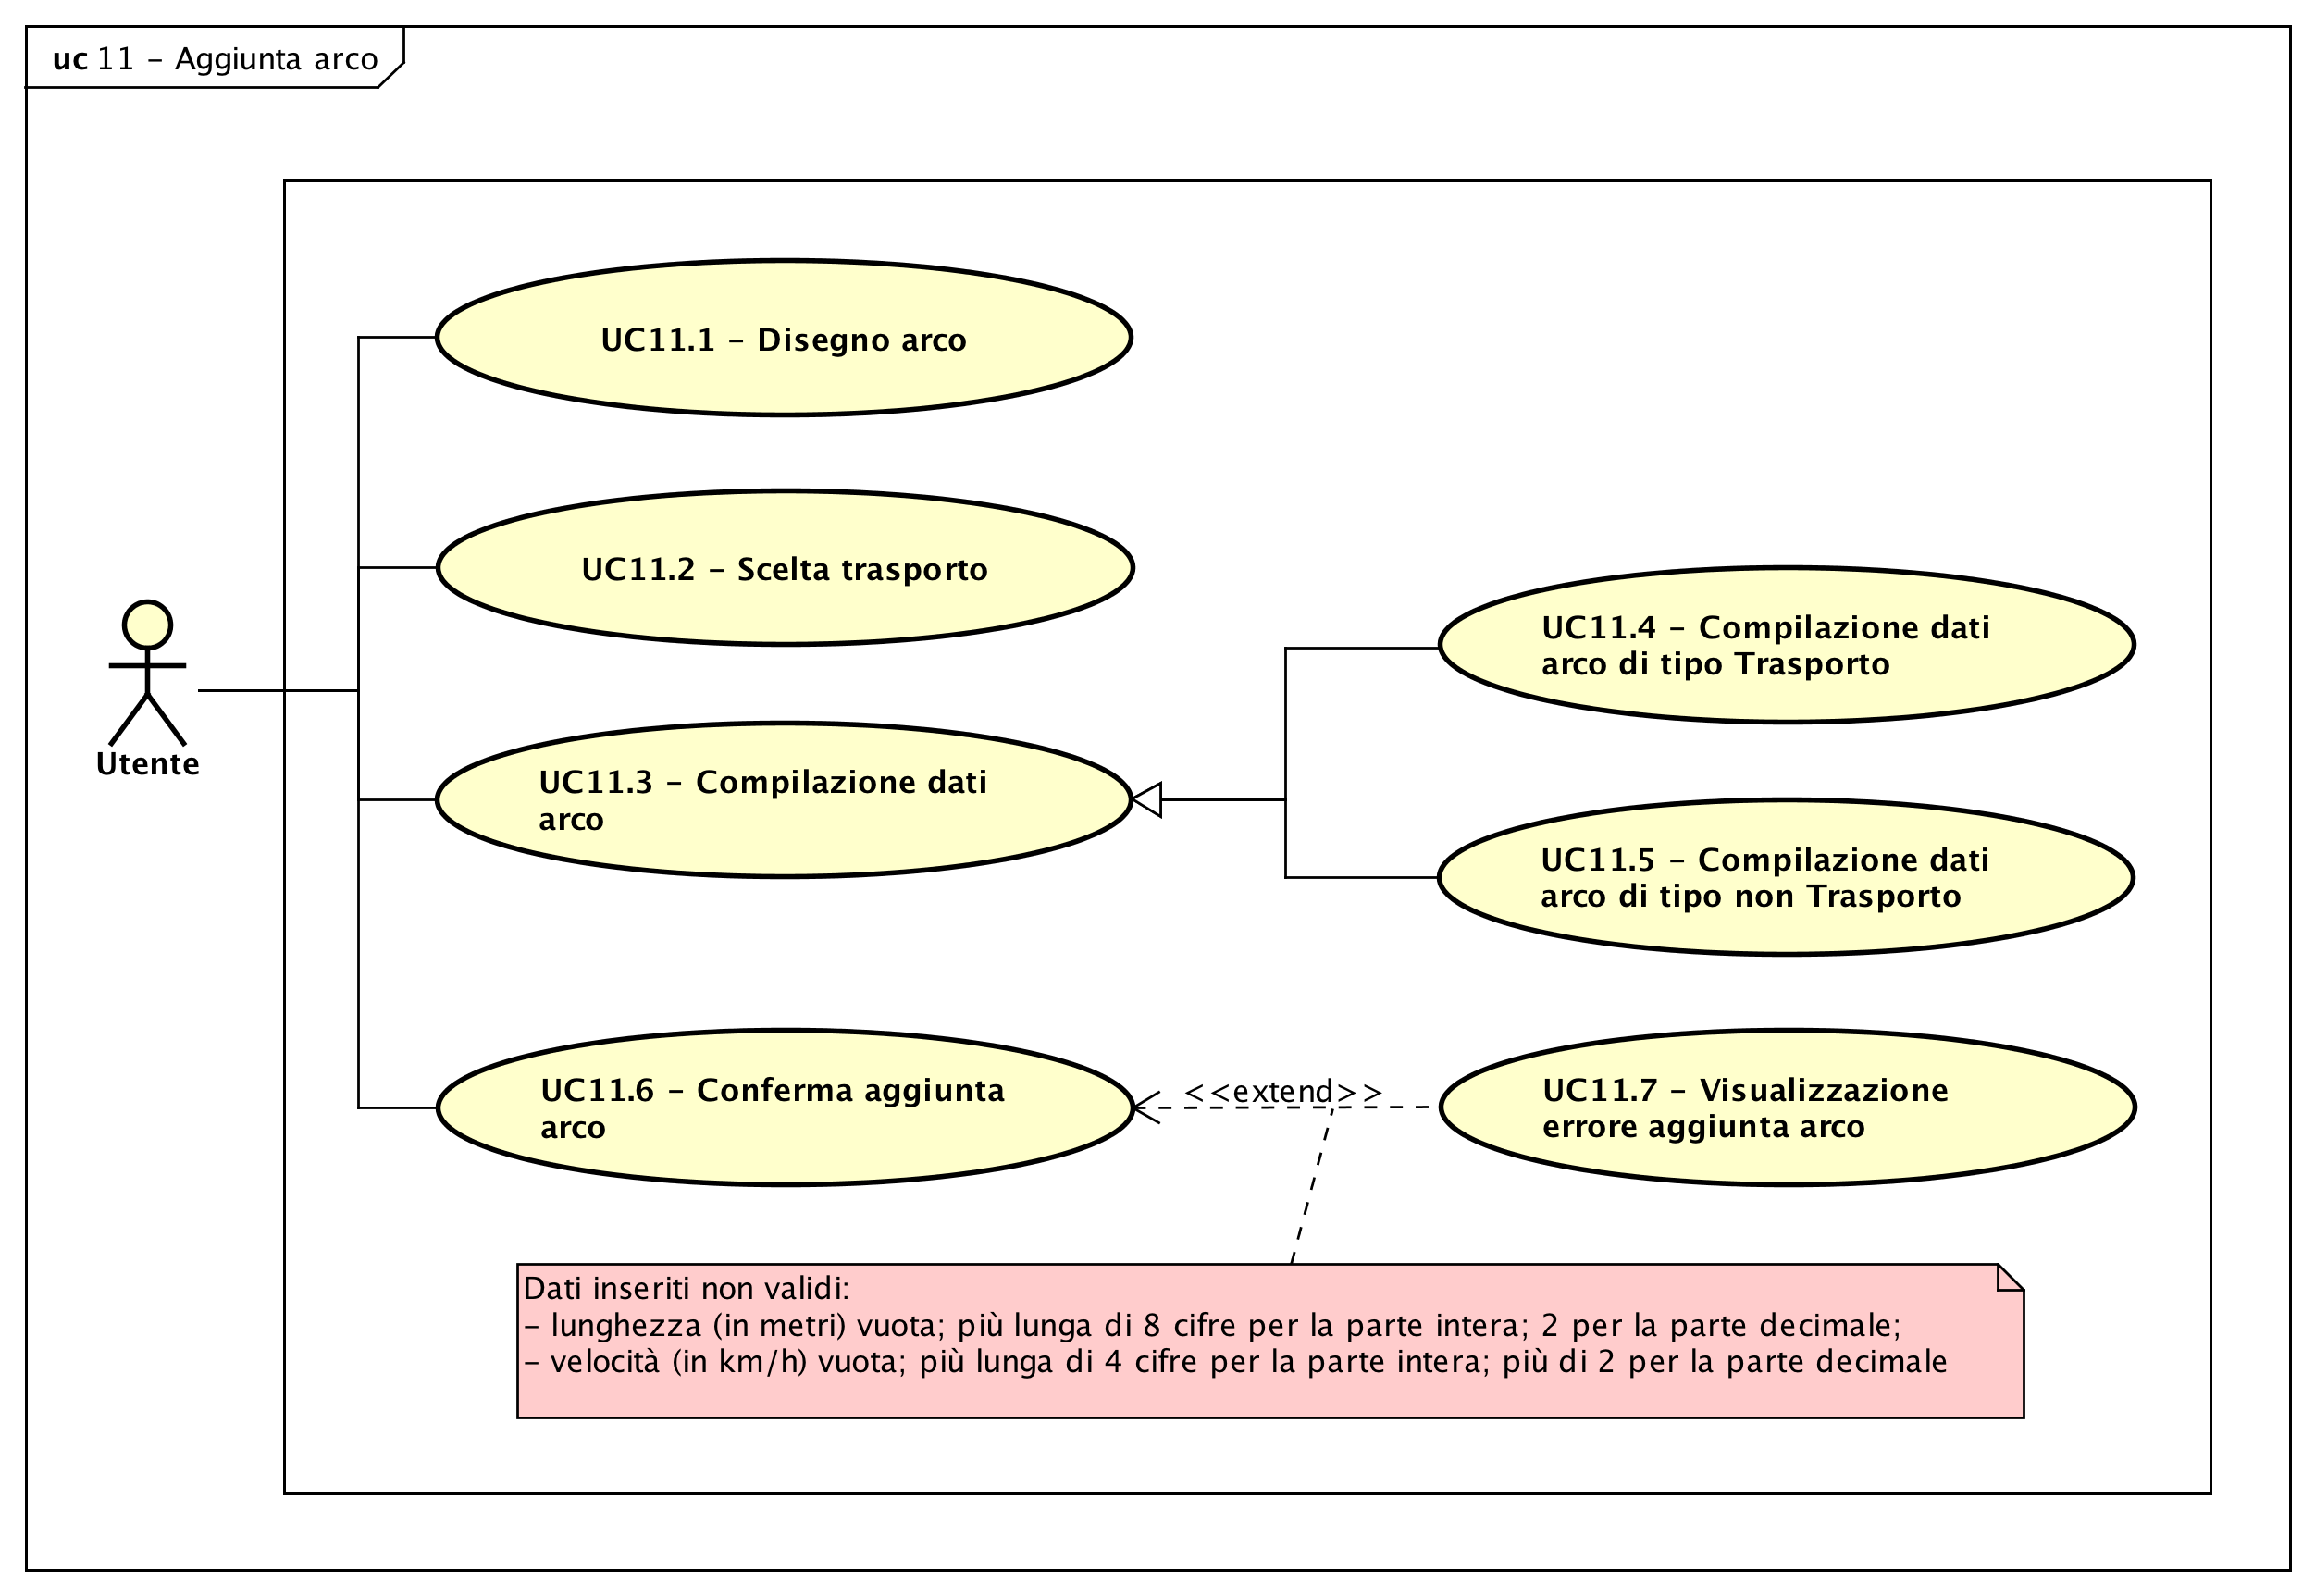
\includegraphics[width=\textwidth]{{img/uc11}.png} 
	\caption{UC11 - Aggiunta arco}
\end{figure}
\def\arraystretch{1.5}
\rowcolors{2}{D}{P}
\begin{tabularx}{\textwidth}{l|p{0.7\textwidth}}
	\rowcolor{I} \multicolumn{2}{c}{\color{white}\textbf{UC11 - Aggiunta arco}} \\
	\toprule
	\endhead
	\textbf{Attori} & Utente\\
	\textbf{Descrizione} & l'utente aggiunge un arco\\
	\textbf{Pre-condizione} & l'utente ha aperto l'applicazione; è stato inserito almeno un nodo\\
	\textbf{Post-condizione} & un nuovo arco è stato aggiunto ed è visualizzabile sulla mappa; l'utente visualizza un messaggio che comunica la corretta esecuzione dell'operazione; l'area informativa rimane impostata sull'arco appena inserito; la posizione e il livello di ingrandimento della mappa rimangono invariati\\
	\textbf{Scenario principale} & \vspace{-1.2em}\begin{enumerate}[leftmargin=*,noitemsep,nosep]
		\item \nameref{sssec:UC11.1};
		\item \nameref{sssec:UC11.2};
		\item \nameref{sssec:UC11.3};
		\item \nameref{sssec:UC11.4};
		\item \nameref{sssec:UC11.5};
		\item \nameref{sssec:UC11.6}.
	\end{enumerate}\\
	\textbf{Estensioni} & \vspace{-1.2em}\begin{itemize}[leftmargin=*,noitemsep,nosep]
		\item \nameref{sssec:UC36}: l'utente interrompe volontariamente l'aggiunta dell'arco
	\end{itemize}\\
	\textbf{Scenari alternativi} & \vspace{-1.2em}\begin{itemize}[leftmargin=*,noitemsep,nosep]
		\item \nameref{sssec:UC11.7}.
	\end{itemize}\\
	%\textbf{Generalizzazioni} &  \\
	\bottomrule
\end{tabularx}
\subsection{UC11.1 - Disegno arco} 
\label{sssec:UC11.1} 
\begin{figure}[H] 
	\centering 
	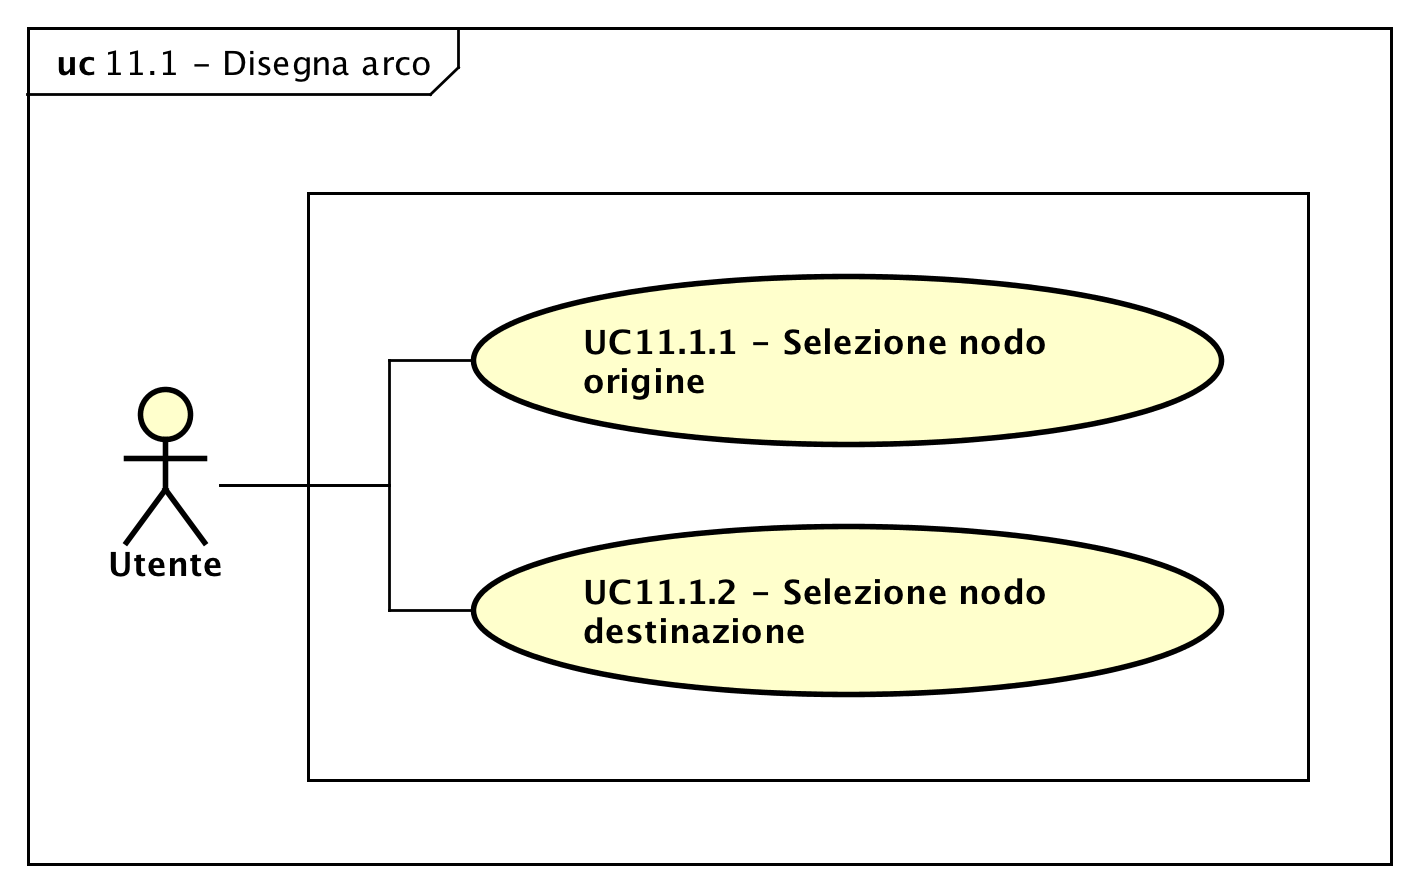
\includegraphics[scale=0.5]{{img/uc11.1}.png} 
	\caption{UC11.1 - Disegno arco}
\end{figure}
\def\arraystretch{1.5}
\rowcolors{2}{D}{P}
\begin{tabularx}{\textwidth}{l|p{0.7\textwidth}}
	\rowcolor{I} \multicolumn{2}{c}{\color{white}\textbf{UC11.1 - Disegno arco}} \\
	\toprule
	\endhead
	\textbf{Attori} & Utente\\
	\textbf{Descrizione} & l'utente disegna un arco\\
	\textbf{Pre-condizione} & esistono almeno due nodi all'interno del sistema\\
	\textbf{Post-condizione} & un arco che collega due nodi è stato disegnato ed è visualizzabile sulla mappa; l'utente può procedere a compilare gli altri dati dell'arco\\
	\textbf{Scenario principale} & \vspace{-1.2em}\begin{enumerate}[leftmargin=*,noitemsep,nosep]
		\item \nameref{sssec:UC11.1.1};
		\item \nameref{sssec:UC11.1.2}.
	\end{enumerate}\\
	%\textbf{Generalizzazioni} &  \\
	\bottomrule
\end{tabularx}
\subsection{UC11.1.1 - Selezione nodo di origine} 
\label{sssec:UC11.1.1} 
\def\arraystretch{1.5}
\rowcolors{2}{D}{P}
\begin{tabularx}{\textwidth}{l|p{0.7\textwidth}}
	\rowcolor{I} \multicolumn{2}{c}{\color{white}\textbf{UC11.1.1 - Selezione nodo di origine}} \\
	\toprule
	\endhead
	\textbf{Attori} & Utente\\
	\textbf{Descrizione} & l'utente seleziona il nodo di origine dell'arco\\
	\textbf{Pre-condizione} & il sistema offre la possibilità di selezionare il nodo di origine\\
	\textbf{Post-condizione} & il nodo di origine è stato selezionato; l'utente può procedere a selezionare il nodo di destinazione\\
	\textbf{Scenario principale} & \vspace{-1.2em}\begin{enumerate}[leftmargin=*,noitemsep,nosep]
		\item \nameref{sssec:UC11.1.1}.
	\end{enumerate}\\
	%\textbf{Generalizzazioni} &  \\
	\bottomrule
\end{tabularx}
\subsection{UC11.1.2 - Selezione nodo di destinazione} 
\label{sssec:UC11.1.2} 
\def\arraystretch{1.5}
\rowcolors{2}{D}{P}
\begin{tabularx}{\textwidth}{l|p{0.7\textwidth}}
	\rowcolor{I} \multicolumn{2}{c}{\color{white}\textbf{UC11.1.2 - Selezione nodo di destinazione}} \\
	\toprule
	\endhead
	\textbf{Attori} & Utente\\
	\textbf{Descrizione} & l'utente seleziona il nodo di destinazione dell'arco\\
	\textbf{Pre-condizione} & il sistema offre la possibilità di selezionare il nodo di destinazione\\
	\textbf{Post-condizione} & il nodo di destinazione è stato selezionato; un arco che collega due nodi è stato disegnato ed è visualizzabile sulla mappa; l'utente può procedere a compilare gli altri dati dell'arco\\
	\textbf{Scenario principale} & \vspace{-1.2em}\begin{enumerate}[leftmargin=*,noitemsep,nosep]
		\item \nameref{sssec:UC11.1.2}.
	\end{enumerate}\\
	%\textbf{Generalizzazioni} &  \\
	\bottomrule
\end{tabularx}
\subsection{UC11.2 - Scelta trasporto} 
\label{sssec:UC11.2} 
\def\arraystretch{1.5}
\rowcolors{2}{D}{P}
\begin{tabularx}{\textwidth}{l|p{0.7\textwidth}}
	\rowcolor{I} \multicolumn{2}{c}{\color{white}\textbf{UC11.2 - Scelta trasporto}} \\
	\toprule
	\endhead
	\textbf{Attori} & Utente\\
	\textbf{Descrizione} & l'utente sceglie se l'arco è di tipo trasporto oppure no\\
	\textbf{Pre-condizione} & il sistema offre la possibilità di specificare se un arco è di tipo trasporto\\
	\textbf{Post-condizione} & l'utente ha scelto se l'arco è di tipo trasporto oppure no; se è di tipo trasporto può visualizzare i dati da compilare relativi all'arco nell'area informativa\\
	\textbf{Scenario principale} & \vspace{-1.2em}\begin{enumerate}[leftmargin=*,noitemsep,nosep]
		\item \nameref{sssec:UC11.2}.
	\end{enumerate}\\
	%\textbf{Generalizzazioni} &  \\
	\bottomrule
\end{tabularx}
\subsection{UC11.3 - Compilazione dati arco} 
\label{sssec:UC11.3} 
\def\arraystretch{1.5}
\rowcolors{2}{D}{P}
\begin{tabularx}{\textwidth}{l|p{0.7\textwidth}}
	\rowcolor{I} \multicolumn{2}{c}{\color{white}\textbf{UC11.3 - Compilazione dati arco}} \\
	\toprule
	\endhead
	\textbf{Attori} & Utente\\
	\textbf{Descrizione} & l'utente compila i dati dell'arco\\
	\textbf{Pre-condizione} & il sistema offre la possibilità di compilare i dati dell'arco\\
	\textbf{Post-condizione} & i dati dell'arco sono stati compilati; l'utente viene riportato alla schermata di aggiunta dell'arco, dove può confermare l'aggiunta\\
		\textbf{Generalizzazioni} &
	\vspace{-1.2em}\begin{enumerate}
		[leftmargin=*,noitemsep,nosep]
		\item \nameref{sssec:UC11.4};
		\item \nameref{sssec:UC11.5}.
	\end{enumerate} \\
	\textbf{Generalizzazioni} &
	\vspace{-1.2em}\begin{itemize}
		[leftmargin=*,noitemsep,nosep]
		\item \nameref{sssec:UC11.4};
		\item \nameref{sssec:UC11.5}.
	\end{itemize} \\
	\bottomrule
\end{tabularx}
\subsection{UC11.4 - Compilazione dati arco di tipo Trasporto} 
\label{sssec:UC11.4} 
\begin{figure}[H] 
	\centering 
	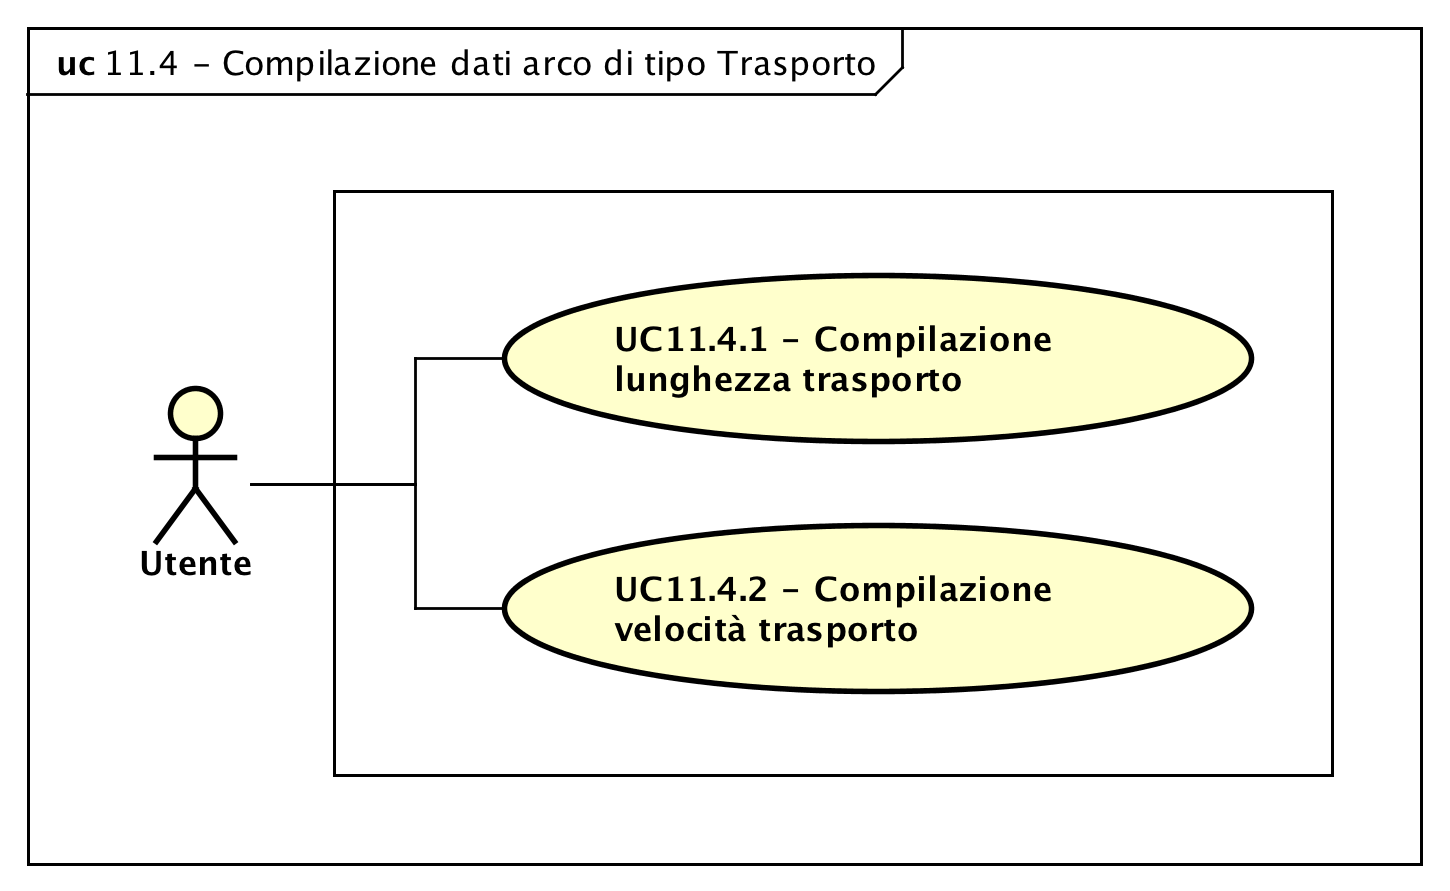
\includegraphics[scale=0.5]{{img/uc11.4}.png} 
	\caption{UC11.4 - Compilazione dati arco di tipo Trasporto}
\end{figure}
\def\arraystretch{1.5}
\rowcolors{2}{D}{P}
\begin{tabularx}{\textwidth}{l|p{0.7\textwidth}}
	\rowcolor{I} \multicolumn{2}{c}{\color{white}\textbf{UC11.4 - Compilazione dati arco di tipo Trasporto}} \\
	\toprule
	\endhead
	\textbf{Attori} & Utente\\
	\textbf{Descrizione} & l'utente compila i dati dell'arco di tipo Trasporto\\
	\textbf{Pre-condizione} & l'utente ha specificato che l'arco è di tipo Trasporto\\
	\textbf{Post-condizione} & i dati dell'arco di tipo Trasporto  sono stati compilati; l'utente viene riportato alla schermata di aggiunta dell'arco, dove può confermare l'aggiunta\\
	\textbf{Scenario principale} & \vspace{-1.2em}\begin{enumerate}[leftmargin=*,noitemsep,nosep]
		\item \nameref{sssec:UC11.4.1};
		\item \nameref{sssec:UC11.4.2}.
	\end{enumerate}\\
	%\textbf{Generalizzazioni} &  \\
	\bottomrule
\end{tabularx}
\subsection{UC11.4.1 - Compilazione lunghezza trasporto} 
\label{sssec:UC11.4.1} 
\def\arraystretch{1.5}
\rowcolors{2}{D}{P}
\begin{tabularx}{\textwidth}{l|p{0.7\textwidth}}
	\rowcolor{I} \multicolumn{2}{c}{\color{white}\textbf{UC11.4.1 - Compilazione lunghezza trasporto}} \\
	\toprule
	\endhead
	\textbf{Attori} & Utente\\
	\textbf{Descrizione} & l'utente compila il campo relativo alla lunghezza del trasporto\\
	\textbf{Pre-condizione} & il sistema offre la possibilità di compilare il campo relativo alla lunghezza del trasporto\\
	\textbf{Post-condizione} & il campo relativo alla lunghezza del trasporto è stato compilato; l'utente visualizza il campo appena compilato nell'area informativa\\
	\textbf{Scenario principale} & \vspace{-1.2em}\begin{enumerate}[leftmargin=*,noitemsep,nosep]
		\item \nameref{sssec:UC11.4.1}.
	\end{enumerate}\\
	%\textbf{Generalizzazioni} &  \\
	\bottomrule
\end{tabularx}
\subsection{UC11.4.2 - Compilazione velocità trasporto} 
\label{sssec:UC11.4.2} 
\def\arraystretch{1.5}
\rowcolors{2}{D}{P}
\begin{tabularx}{\textwidth}{l|p{0.7\textwidth}}
	\rowcolor{I} \multicolumn{2}{c}{\color{white}\textbf{UC11.4.2 - Compilazione velocità trasporto}} \\
	\toprule
	\endhead
	\textbf{Attori} & Utente\\
	\textbf{Descrizione} & l'utente compila il campo relativo alla velocità del trasporto\\
	\textbf{Pre-condizione} & il sistema offre la possibilità di compilare il campo relativo alla velocità del trasporto\\
	\textbf{Post-condizione} & il campo relativo alla lunghezza del trasporto è stato compilato; l'utente visualizza il campo appena compilato nell'area informativa\\
	\textbf{Scenario principale} & \vspace{-1.2em}\begin{enumerate}[leftmargin=*,noitemsep,nosep]
		\item \nameref{sssec:UC11.4.2}.
	\end{enumerate}\\
	%\textbf{Generalizzazioni} &  \\
	\bottomrule
\end{tabularx}
\subsection{UC11.5 - Compilazione dati arco di tipo non Trasporto} 
\label{sssec:UC11.5} 
\def\arraystretch{1.5}
\rowcolors{2}{D}{P}
\begin{tabularx}{\textwidth}{l|p{0.7\textwidth}}
	\rowcolor{I} \multicolumn{2}{c}{\color{white}\textbf{UC11.5 - Compilazione dati arco di tipo non Trasporto}} \\
	\toprule
	\endhead
	\textbf{Attori} & Utente\\
	\textbf{Descrizione} & l'utente compila i dati dell'arco di tipo non Trasporto\\
	\textbf{Pre-condizione} & l'utente ha disegnato l'arco; l'utente ha specificato che l'arco è di tipo non Trasporto\\
	\textbf{Post-condizione} & i dati dell'arco di tipo non Trasporto sono stati compilati; l'utente viene riportato alla schermata di aggiunta dell'arco, dove può confermare l'aggiunta\\
	\textbf{Scenario principale} & \vspace{-1.2em}\begin{enumerate}[leftmargin=*,noitemsep,nosep]
		\item \nameref{sssec:UC11.5}.
	\end{enumerate}\\
	%\textbf{Generalizzazioni} &  \\
	\bottomrule
\end{tabularx}
\subsection{UC11.6 - Conferma aggiunta arco} 
\label{sssec:UC11.6} 
\def\arraystretch{1.5}
\rowcolors{2}{D}{P}
\begin{tabularx}{\textwidth}{l|p{0.7\textwidth}}
	\rowcolor{I} \multicolumn{2}{c}{\color{white}\textbf{UC11.6 - Conferma aggiunta arco}} \\
	\toprule
	\endhead
	\textbf{Attori} & Utente\\
	\textbf{Descrizione} & l'utente conferma l'aggiunta dell'arco\\
	\textbf{Pre-condizione} & il sistema offre la possibilità di confermare l'aggiunta dell'arco\\
	\textbf{Post-condizione} & un nuovo arco è stato aggiunto ed è visualizzabile sulla mappa; l'utente visualizza un messaggio che comunica la corretta esecuzione dell'operazione; l'area informativa rimane impostata sull'arco appena inserito; la posizione e il livello di ingrandimento della mappa rimangono invariati\\
	\textbf{Scenario principale} & \vspace{-1.2em}\begin{enumerate}[leftmargin=*,noitemsep,nosep]
		\item \nameref{sssec:UC11.6}.
	\end{enumerate}\\
	\textbf{Estensioni} & \vspace{-1.2em}\begin{itemize}[leftmargin=*,noitemsep,nosep]
		\item \nameref{sssec:UC11.7}: dati inseriti non validi:
		\begin{itemize}
			\item lunghezza (in metri) vuota;
			più lunga di 8 cifre per la parte intera; 2 per la parte
			decimale;
			\item velocità (in km/h) vuota; più
			lunga di 4 cifre per la parte intera; più di 2 per la parte
			decimale.
		\end{itemize} 
	\end{itemize}\\
	%\textbf{Generalizzazioni} &  \\
	\bottomrule
\end{tabularx}
\subsection{UC11.7 - Visualizzazione errore aggiunta arco} 
\label{sssec:UC11.7} 
\def\arraystretch{1.5}
\rowcolors{2}{D}{P}
\begin{tabularx}{\textwidth}{l|p{0.7\textwidth}}
	\rowcolor{I} \multicolumn{2}{c}{\color{white}\textbf{UC11.7 - Visualizzazione errore aggiunta arco}} \\
	\toprule
	\endhead
	\textbf{Attori} & Utente\\
	\textbf{Descrizione} & l'utente visualizza un errore relativo ai dati dell'arco compilati in modo errato\\
	\textbf{Pre-condizione} & l'utente sta tentando di inserire un nuovo arco\\
	\textbf{Post-condizione} & nessun nuovo arco inserito; l'utente visualizza un errore relativo ai dati dell'arco compilati in modo errato; l'utente viene riportato alla schermata di aggiunta arco\\
	\textbf{Scenario principale} & \vspace{-1.2em}\begin{enumerate}[leftmargin=*,noitemsep,nosep]
		\item \nameref{sssec:UC11.7}.
	\end{enumerate}\\
	%\textbf{Generalizzazioni} &  \\
	\bottomrule
\end{tabularx}
\subsection{UC12 - Visualizzazione info arco} 
\label{sssec:UC12} 
\def\arraystretch{1.5}
\rowcolors{2}{D}{P}
\begin{tabularx}{\textwidth}{l|p{0.7\textwidth}}
	\rowcolor{I} \multicolumn{2}{c}{\color{white}\textbf{UC12 - Visualizzazione info arco}} \\
	\toprule
	\endhead
	\textbf{Attori} & Utente\\
	\textbf{Descrizione} & l'utente seleziona un arco e ne visualizza le informazioni\\
	\textbf{Pre-condizione} & l'utente ha aperto l'applicazione, è stato inserito almeno un arco\\
	\textbf{Post-condizione} & il sistema mostra nell'area informativa le informazioni dell'arco selezionato; la posizione e il livello di ingrandimento della mappa rimangono invariati\\
	\textbf{Scenario principale} & \vspace{-1.2em}\begin{enumerate}[leftmargin=*,noitemsep,nosep]
		\item \nameref{sssec:UC12}.
	\end{enumerate}\\
	%\textbf{Generalizzazioni} &  \\
	\bottomrule
\end{tabularx}
\subsection{UC13 - Chiusura visualizzazione info arco} 
\label{sssec:UC13} 
\def\arraystretch{1.5}
\rowcolors{2}{D}{P}
\begin{tabularx}{\textwidth}{l|p{0.7\textwidth}}
	\rowcolor{I} \multicolumn{2}{c}{\color{white}\textbf{UC13 - Chiusura visualizzazione info arco}} \\
	\toprule
	\endhead
	\textbf{Attori} & Utente\\
	\textbf{Descrizione} & l'utente chiude la visualizzazione delle informazioni di un arco\\
	\textbf{Pre-condizione} & l'utente ha visualizzato le informazioni di un arco\\
	\textbf{Post-condizione} & è stata chiusa la visualizzazione delle informazioni dell'arco selezionato nell'area informativa; l'area informativa viene impostata sulla visualizzazione di default; la posizione e il livello di ingrandimento della mappa rimangono invariati\\
	\textbf{Scenario principale} & \vspace{-1.2em}\begin{enumerate}[leftmargin=*,noitemsep,nosep]
		\item \nameref{sssec:UC13}.
	\end{enumerate}\\
	%\textbf{Generalizzazioni} &  \\
	\bottomrule
\end{tabularx}
\subsection{UC14 - Modifica arco} 
\label{sssec:UC14} 
\begin{figure}[H] 
	\centering 
	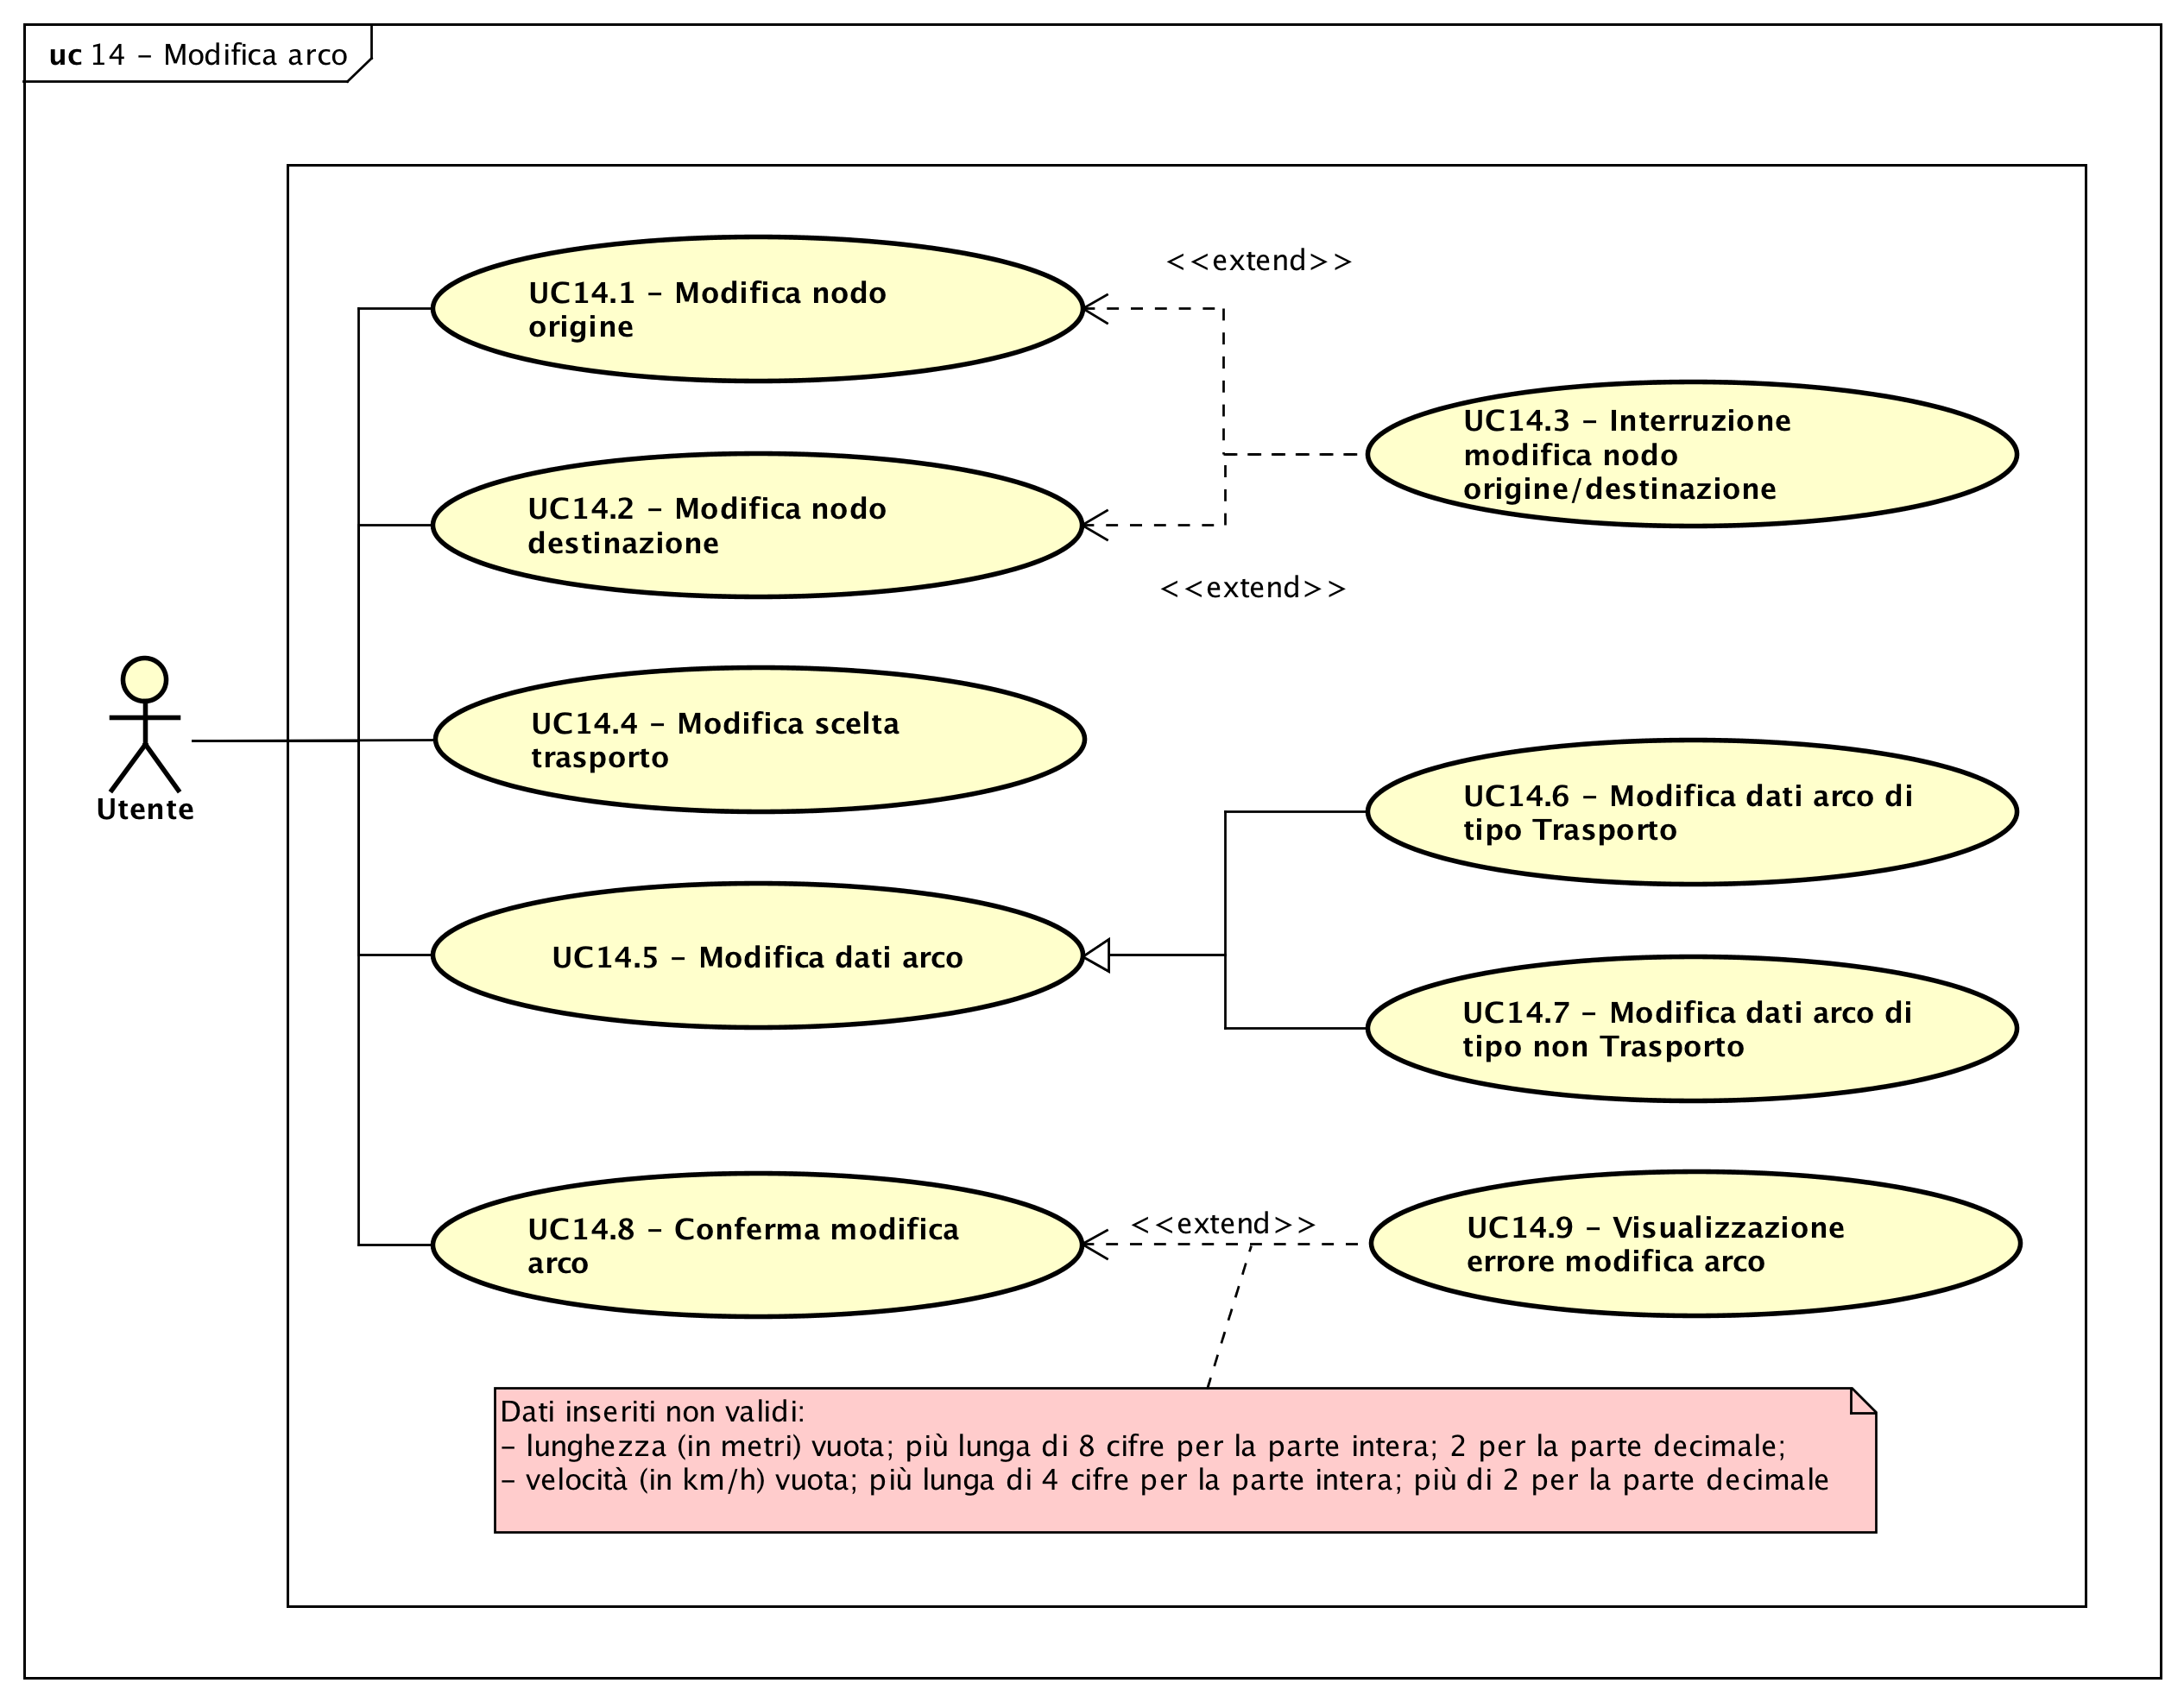
\includegraphics[width=\textwidth]{{img/uc14}.png} 
	\caption{UC14 - Modifica arco}
\end{figure}
\def\arraystretch{1.5}
\rowcolors{2}{D}{P}
\begin{tabularx}{\textwidth}{l|p{0.7\textwidth}}
	\rowcolor{I} \multicolumn{2}{c}{\color{white}\textbf{UC14 - Modifica arco}} \\
	\toprule
	\endhead
	\textbf{Attori} & Utente\\
	\textbf{Descrizione} & l'utente modifica l'arco\\
	\textbf{Pre-condizione} & l'utente ha aperto l'applicazione; almeno un arco è stato aggiunto; l'utente ha selezionato un arco\\
	\textbf{Post-condizione} & l'arco è stato modificato; l'utente visualizza un messaggio che comunica la corretta esecuzione dell'operazione; l'area informativa rimane impostata sull'arco appena modificato; la posizione e il livello di ingrandimento della mappa rimangono invariati\\
	\textbf{Scenario principale} & \vspace{-1.2em}\begin{enumerate}[leftmargin=*,noitemsep,nosep]
		\item \nameref{sssec:UC14.1};
		\item \nameref{sssec:UC14.2};
		\item \nameref{sssec:UC14.4};
		\item \nameref{sssec:UC14.5};
		\item \nameref{sssec:UC14.6};
		\item \nameref{sssec:UC14.7};
		\item \nameref{sssec:UC14.8}.
	\end{enumerate}\\
	\textbf{Estensioni} & \vspace{-1.2em}\begin{itemize}[leftmargin=*,noitemsep,nosep]
		\item \nameref{sssec:UC37}: l'utente interrompe volontariamente la modifica dei dati
		dell'arco;
	\end{itemize}\\
	\textbf{Scenari alternativi} & \vspace{-1.2em}\begin{itemize}[leftmargin=*,noitemsep,nosep]
		\item \nameref{sssec:UC14.3};
		\item \nameref{sssec:UC14.9}.
	\end{itemize}\\
	%\textbf{Generalizzazioni} &  \\
	\bottomrule
\end{tabularx}
\subsection{UC14.1 - Modifica nodo origine} 
\label{sssec:UC14.1} 
\def\arraystretch{1.5}
\rowcolors{2}{D}{P}
\begin{tabularx}{\textwidth}{l|p{0.7\textwidth}}
	\rowcolor{I} \multicolumn{2}{c}{\color{white}\textbf{UC14.1 - Modifica nodo origine}} \\
	\toprule
	\endhead
	\textbf{Attori} & Utente\\
	\textbf{Descrizione} & l'utente modifica il nodo di origine dell'arco\\
	\textbf{Pre-condizione} & il sistema offre la possibilità di modificare il nodo di origine\\
	\textbf{Post-condizione} & il nodo di origine è stato modificato; l'arco parte dal nuovo nodo di origine indicato; l'utente viene riportato alla schermata di modifica arco\\
	\textbf{Scenario principale} & \vspace{-1.2em}\begin{enumerate}[leftmargin=*,noitemsep,nosep]
		\item \nameref{sssec:UC14.1}.
	\end{enumerate}\\
	\textbf{Estensioni} & \vspace{-1.2em}\begin{itemize}[leftmargin=*,noitemsep,nosep]
		\item \nameref{sssec:UC14.3}: l'utente interrompe volontariamente la modifica del nodo di
		origine/destinazione dell'arco
	\end{itemize}\\
	%\textbf{Generalizzazioni} &  \\
	\bottomrule
\end{tabularx}
\subsection{UC14.2 - Modifica nodo destinazione} 
\label{sssec:UC14.2} 
\def\arraystretch{1.5}
\rowcolors{2}{D}{P}
\begin{tabularx}{\textwidth}{l|p{0.7\textwidth}}
	\rowcolor{I} \multicolumn{2}{c}{\color{white}\textbf{UC14.2 - Modifica nodo destinazione}} \\
	\toprule
	\endhead
	\textbf{Attori} & Utente\\
	\textbf{Descrizione} & l'utente modifica il nodo di destinazione dell'arco\\
	\textbf{Pre-condizione} & il sistema offre la possibilità di modificare il nodo di destinazione\\
	\textbf{Post-condizione} & il nodo di destinazione è stato modificato; l'arco arriva nel nuovo nodo di destinazione indicato; l'utente viene riportato alla schermata di modifica arco\\
	\textbf{Scenario principale} & \vspace{-1.2em}\begin{enumerate}[leftmargin=*,noitemsep,nosep]
		\item \nameref{sssec:UC14.2}.
	\end{enumerate}\\
	\textbf{Estensioni} & \vspace{-1.2em}\begin{itemize}[leftmargin=*,noitemsep,nosep]
		\item \nameref{sssec:UC14.3}: l'utente interrompe volontariamente la modifica del nodo di
		origine/destinazione dell'arco;
	\end{itemize}\\
	%\textbf{Generalizzazioni} &  \\
	\bottomrule
\end{tabularx}
\subsection{UC14.3 - Interruzione modifica nodo origine/destinazione} 
\label{sssec:UC14.3} 
\def\arraystretch{1.5}
\rowcolors{2}{D}{P}
\begin{tabularx}{\textwidth}{l|p{0.7\textwidth}}
	\rowcolor{I} \multicolumn{2}{c}{\color{white}\textbf{UC14.3 - Interruzione modifica nodo origine/destinazione}} \\
	\toprule
	\endhead
	\textbf{Attori} & Utente\\
	\textbf{Descrizione} & l'utente interrompe la modifica del nodo di origine o di destinazione\\
	\textbf{Pre-condizione} & il sistema offre la possibilità di modificare il nodo di origine o di destinazione\\
	\textbf{Post-condizione} & il nodo di origine o di destinazione non è stato modificato; l'utente viene riportato alla schermata di modifica arco\\
	\textbf{Scenario principale} & \vspace{-1.2em}\begin{enumerate}[leftmargin=*,noitemsep,nosep]
		\item \nameref{sssec:UC14.3}
	\end{enumerate}\\
	%\textbf{Generalizzazioni} &  \\
	\bottomrule
\end{tabularx}
\subsection{UC14.4 - Modifica scelta trasporto} 
\label{sssec:UC14.4} 
\def\arraystretch{1.5}
\rowcolors{2}{D}{P}
\begin{tabularx}{\textwidth}{l|p{0.7\textwidth}}
	\rowcolor{I} \multicolumn{2}{c}{\color{white}\textbf{UC14.4 - Modifica scelta trasporto}} \\
	\toprule
	\endhead
	\textbf{Attori} & Utente\\
	\textbf{Descrizione} & l'utente modifica la scelta riguardo il trasporto\\
	\textbf{Pre-condizione} & il sistema offre la possibilità di modificare la scelta riguardo il trasporto\\
	\textbf{Post-condizione} & la scelta riguardo il trasporto è stata modificata; l'utente visualizza la nuova scelta nell'area informativa\\
	\textbf{Scenario principale} & \vspace{-1.2em}\begin{enumerate}[leftmargin=*,noitemsep,nosep]
		\item \nameref{sssec:UC14.4}.
	\end{enumerate}\\
	%\textbf{Generalizzazioni} &  \\
	\bottomrule
\end{tabularx}
\subsection{UC14.5 - Modifica dati arco} 
\label{sssec:UC14.5} 
\def\arraystretch{1.5}
\rowcolors{2}{D}{P}
\begin{tabularx}{\textwidth}{l|p{0.7\textwidth}}
	\rowcolor{I} \multicolumn{2}{c}{\color{white}\textbf{UC14.5 - Modifica dati arco}} \\
	\toprule
	\endhead
	\textbf{Attori} & Utente\\
	\textbf{Descrizione} & l'utente modifica i dati dell'arco\\
	\textbf{Pre-condizione} & l'utente ha specificato che l'arco è di tipo trasporto\\
	\textbf{Post-condizione} & l'utente ha modificato i dati dell'arco e li può visualizzare nell'area informativa; l'utente viene riportato alla schermata di modifica dell'arco\\
	\textbf{Generalizzazioni} &
	\vspace{-1.2em}\begin{enumerate}
		[leftmargin=*,noitemsep,nosep]
		\item \nameref{sssec:UC14.6};
		\item \nameref{sssec:UC14.7}.
	\end{enumerate} \\
\textbf{Generalizzazioni} &
\vspace{-1.2em}\begin{itemize}
	[leftmargin=*,noitemsep,nosep]
	\item \nameref{sssec:UC14.6};
	\item \nameref{sssec:UC14.7}.
\end{itemize} \\
	\bottomrule
\end{tabularx}


\subsection{UC14.6 - Modifica dati arco di tipo Trasporto} 
\label{sssec:UC14.6} 
\begin{figure}[H] 
	\centering 
	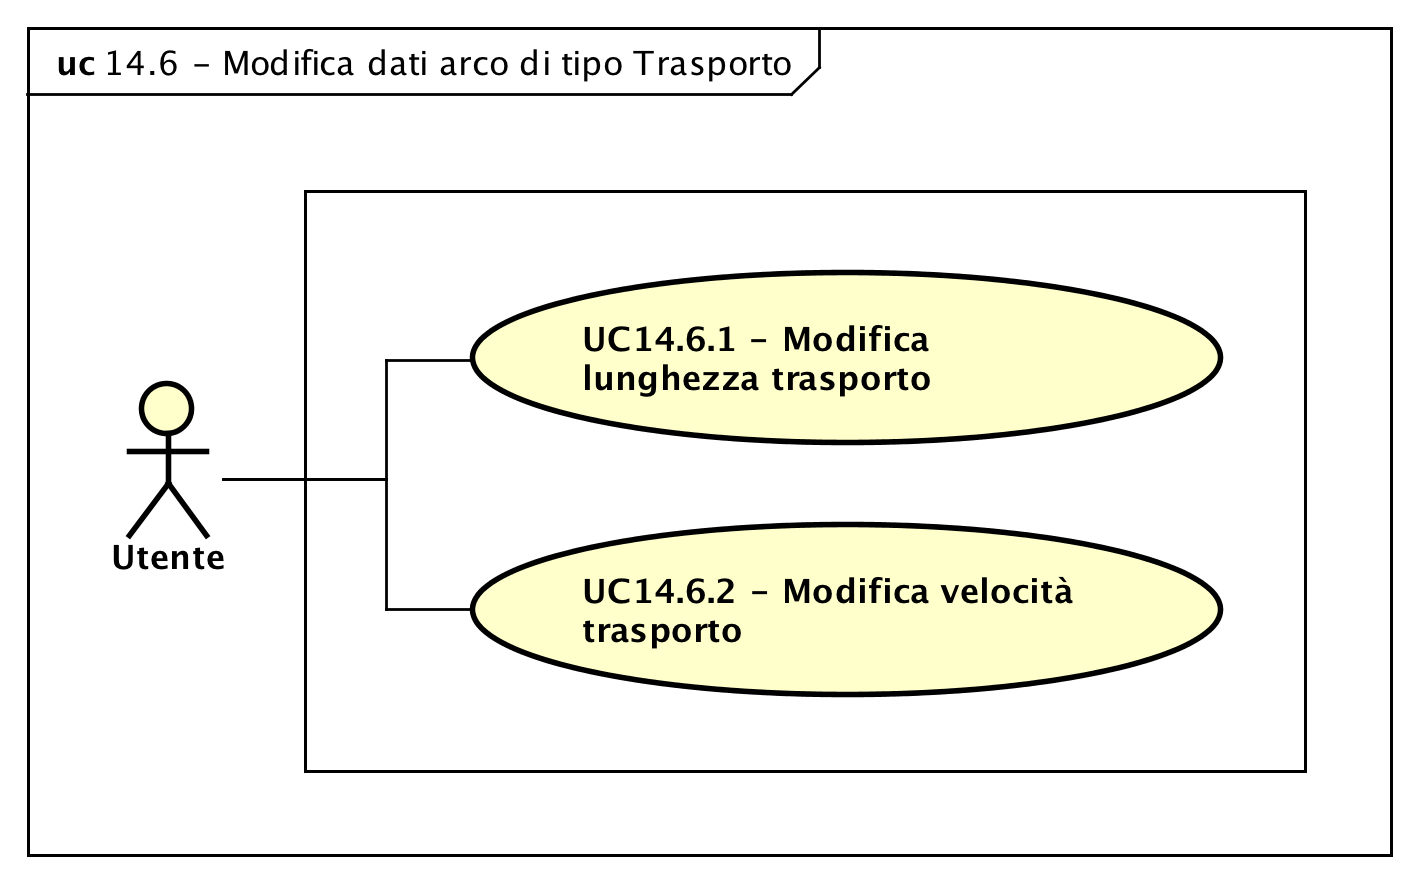
\includegraphics[scale=0.5]{{img/uc14.6}.png} 
	\caption{UC14.6 - Modifica dati arco di tipo Trasporto}
\end{figure}
\def\arraystretch{1.5}
\rowcolors{2}{D}{P}
\begin{tabularx}{\textwidth}{l|p{0.7\textwidth}}
	\rowcolor{I} \multicolumn{2}{c}{\color{white}\textbf{UC14.6 - Modifica dati arco di tipo Trasporto}} \\
	\toprule
	\endhead
	\textbf{Attori} & Utente\\
	\textbf{Descrizione} & l'utente modifica i dati dell'arco di tipo Trasporto\\
	\textbf{Pre-condizione} & l'utente ha specificato che l'arco è di tipo Trasporto\\
	\textbf{Post-condizione} & l'utente ha modificato i dati dell'arco di tipo Trasporto e li può visualizzare nell'area informativa; l'utente viene riportato alla schermata di modifica dell'arco\\
	\textbf{Scenario principale} & \vspace{-1.2em}\begin{enumerate}[leftmargin=*,noitemsep,nosep]
		\item \nameref{sssec:UC14.6.1};
		\item \nameref{sssec:UC14.6.2}.
	\end{enumerate}\\
	%\textbf{Generalizzazioni} &  \\
	\bottomrule
\end{tabularx}
\subsection{UC14.6.1 - Modifica lunghezza trasporto} 
\label{sssec:UC14.6.1} 
\def\arraystretch{1.5}
\rowcolors{2}{D}{P}
\begin{tabularx}{\textwidth}{l|p{0.7\textwidth}}
	\rowcolor{I} \multicolumn{2}{c}{\color{white}\textbf{UC14.6.1 - Modifica lunghezza trasporto}} \\
	\toprule
	\endhead
	\textbf{Attori} & Utente\\
	\textbf{Descrizione} & l'utente modifica la lunghezza del trasporto\\
	\textbf{Pre-condizione} & il sistema offre la possibilità di modificare la lunghezza del trasporto; l'utente ha specificato che il nodo è di tipo trasporto\\
	\textbf{Post-condizione} & la lunghezza del trasporto è stata modificata; l'utente visualizza la lunghezza appena inserita nell'area informativa\\
	\textbf{Scenario principale} & \vspace{-1.2em}\begin{enumerate}[leftmargin=*,noitemsep,nosep]
		\item \nameref{sssec:UC14.6.1}.
	\end{enumerate}\\
	%\textbf{Generalizzazioni} &  \\
	\bottomrule
\end{tabularx}
\subsection{UC14.6.2 - Modifica velocità trasporto} 
\label{sssec:UC14.6.2} 
\def\arraystretch{1.5}
\rowcolors{2}{D}{P}
\begin{tabularx}{\textwidth}{l|p{0.7\textwidth}}
	\rowcolor{I} \multicolumn{2}{c}{\color{white}\textbf{UC14.6.2 - Modifica velocità trasporto}} \\
	\toprule
	\endhead
	\textbf{Attori} & Utente\\
	\textbf{Descrizione} & l'utente modifica la velocità del trasporto\\
	\textbf{Pre-condizione} & il sistema offre la possibilità di modificare la velocità del trasporto; l'utente ha specificato che il nodo è di tipo trasporto\\
	\textbf{Post-condizione} & la velocità del trasporto è stata modificata; l'utente visualizza la nuova velocità appena inserita nell'area informativa\\
	\textbf{Scenario principale} & \vspace{-1.2em}\begin{enumerate}[leftmargin=*,noitemsep,nosep]
		\item \nameref{sssec:UC14.6.2}.
	\end{enumerate}\\
	%\textbf{Generalizzazioni} &  \\
	\bottomrule
\end{tabularx}
\subsection{UC14.7 - Modifica dati arco di tipo non Trasporto} 
\label{sssec:UC14.7} 
\def\arraystretch{1.5}
\rowcolors{2}{D}{P}
\begin{tabularx}{\textwidth}{l|p{0.7\textwidth}}
	\rowcolor{I} \multicolumn{2}{c}{\color{white}\textbf{UC14.7 - Modifica dati arco di tipo non Trasporto}} \\
	\toprule
	\endhead
	\textbf{Attori} & Utente\\
	\textbf{Descrizione} & l'utente modifica i dati dell'arco di tipo non Trasporto\\
	\textbf{Pre-condizione} & l'utente ha specificato che l'arco è di tipo non Trasporto\\
	\textbf{Post-condizione} & l'utente ha modificato i dati dell'arco di tipo non Trasporto e li può visualizzare nell'area informativa; l'utente viene riportato alla schermata di modifica dell'arco\\
	\textbf{Scenario principale} & \vspace{-1.2em}\begin{enumerate}[leftmargin=*,noitemsep,nosep]
		\item \nameref{sssec:UC14.7}.
	\end{enumerate}\\
	%\textbf{Generalizzazioni} &  \\
	\bottomrule
\end{tabularx}
\subsection{UC14.8 - Conferma modifica arco} 
\label{sssec:UC14.8} 
\def\arraystretch{1.5}
\rowcolors{2}{D}{P}
\begin{tabularx}{\textwidth}{l|p{0.7\textwidth}}
	\rowcolor{I} \multicolumn{2}{c}{\color{white}\textbf{UC14.8 - Conferma modifica arco}} \\
	\toprule
	\endhead
	\textbf{Attori} & Utente\\
	\textbf{Descrizione} & l'utente conferma la modifica dell'arco\\
	\textbf{Pre-condizione} & il sistema offre la possibilità di confermare la modifica dell'arco\\
	\textbf{Post-condizione} & l'arco è stato modificato;  l'utente visualizza un messaggio che comunica la corretta esecuzione dell'operazione; l'area informativa rimane impostata sull'arco appena modificato; la posizione e il livello di ingrandimento della mappa rimangono invariati\\
	\textbf{Scenario principale} & \vspace{-1.2em}\begin{enumerate}[leftmargin=*,noitemsep,nosep]
		\item \nameref{sssec:UC14.8}.
	\end{enumerate}\\
	\textbf{Estensioni} & \vspace{-1.2em}\begin{itemize}[leftmargin=*,noitemsep,nosep]
		\item \nameref{sssec:UC14.9}: dati inseriti non validi:
		\begin{itemize}
			\item lunghezza (in metri) vuota;
			più lunga di 8 cifre per la parte intera; 2 per la parte
			decimale;
			\item velocità (in km/h) vuota; più
			lunga di 4 cifre per la parte intera; più di 2 per la parte
			decimale.
		\end{itemize}
	\end{itemize}\\
	%\textbf{Generalizzazioni} &  \\
	\bottomrule
\end{tabularx}
\subsection{UC14.9 - Visualizzazione errore modifica arco} 
\label{sssec:UC14.9} 
\def\arraystretch{1.5}
\rowcolors{2}{D}{P}
\begin{tabularx}{\textwidth}{l|p{0.7\textwidth}}
	\rowcolor{I} \multicolumn{2}{c}{\color{white}\textbf{UC14.9 - Visualizzazione errore modifica arco}} \\
	\toprule
	\endhead
	\textbf{Attori} & Utente\\
	\textbf{Descrizione} & l'utente visualizza un errore relativo alla modifica dell'arco\\
	\textbf{Pre-condizione} & l'utente ha confermato la modifica dell'arco\\
	\textbf{Post-condizione} & l'arco non è stato modificato; l'utente visualizza un errore relativo ai dati del nodo compilati in modo errato; l'utente viene riportato alla schermata di modifica nodo\\
	\textbf{Scenario principale} & \vspace{-1.2em}\begin{enumerate}[leftmargin=*,noitemsep,nosep]
		\item \nameref{sssec:UC14.9}.
	\end{enumerate}\\
	%\textbf{Generalizzazioni} &  \\
	\bottomrule
\end{tabularx}
\subsection{UC15 - Eliminazione arco} 
\label{sssec:UC15} 
\begin{figure}[H] 
	\centering 
	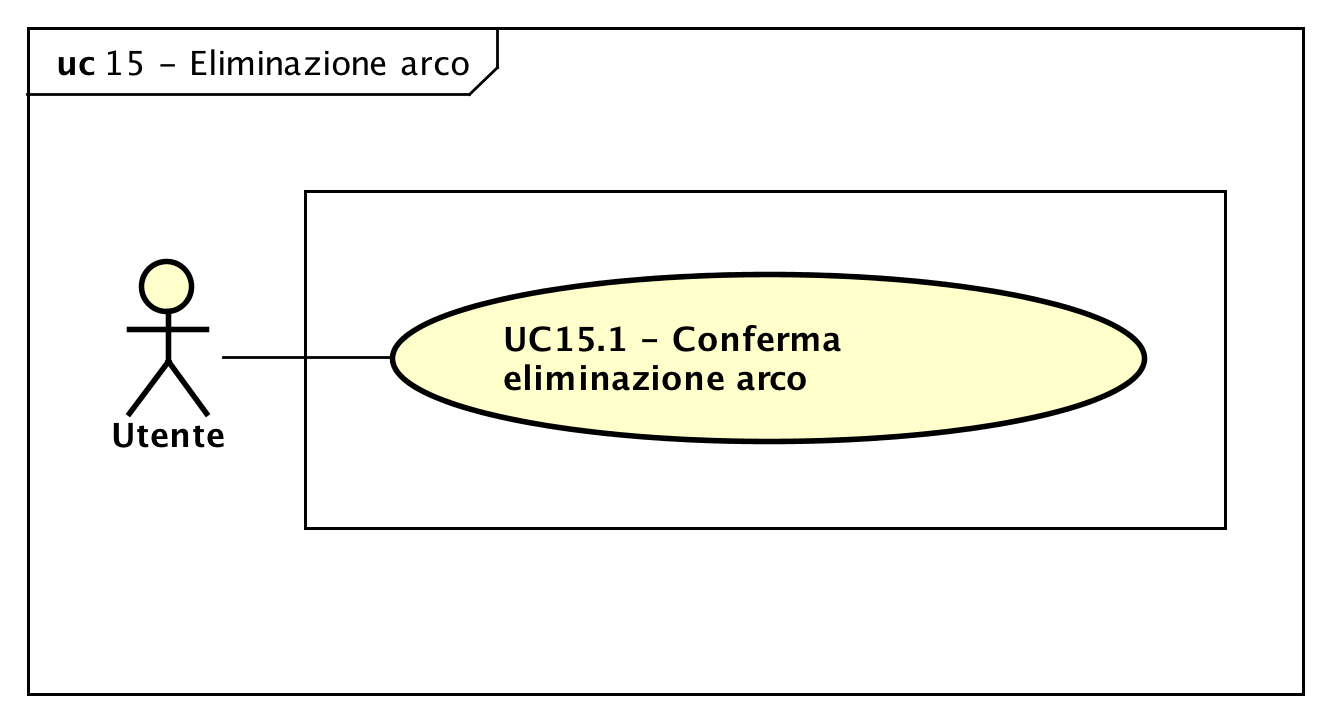
\includegraphics[scale=0.5]{{img/uc15}.png} 
	\caption{UC15 - Eliminazione arco}
\end{figure}
\def\arraystretch{1.5}
\rowcolors{2}{D}{P}
\begin{tabularx}{\textwidth}{l|p{0.7\textwidth}}
	\rowcolor{I} \multicolumn{2}{c}{\color{white}\textbf{UC15 - Eliminazione arco}} \\
	\toprule
	\endhead
	\textbf{Attori} & Utente\\
	\textbf{Descrizione} & l'utente elimina un arco\\
	\textbf{Pre-condizione} & l'utente ha aperto l'applicazione; è stato inserito almeno un arco; l'utente ha selezionato un arco\\
	\textbf{Post-condizione} & l'arco è stato eliminato e non è più visualizzato sulla mappa; l'utente visualizza un messaggio che comunica la corretta esecuzione dell'operazione; l'area informativa viene impostata sulla visualizzazione di default;  la posizione e il livello di ingrandimento della mappa rimangono invariati\\
	\textbf{Scenario principale} & \vspace{-1.2em}\begin{enumerate}[leftmargin=*,noitemsep,nosep]
		\item \nameref{sssec:UC15.1}.
	\end{enumerate}\\
	\textbf{Estensioni} & \vspace{-1.2em}\begin{itemize}[leftmargin=*,noitemsep,nosep]
		\item \nameref{sssec:UC38}: l'utente interrompe volontariamente l'eliminazione
		dell'arco
	\end{itemize}\\
	%\textbf{Generalizzazioni} &  \\
	\bottomrule
\end{tabularx}
\subsection{UC15.1 - Conferma eliminazione arco} 
\label{sssec:UC15.1} 
\def\arraystretch{1.5}
\rowcolors{2}{D}{P}
\begin{tabularx}{\textwidth}{l|p{0.7\textwidth}}
	\rowcolor{I} \multicolumn{2}{c}{\color{white}\textbf{UC15.1 - Conferma eliminazione arco}} \\
	\toprule
	\endhead
	\textbf{Attori} & Utente\\
	\textbf{Descrizione} & l'utente conferma l'eliminazione dell'arco\\
	\textbf{Pre-condizione} & il sistema offre la possibilità di confermare l'eliminazione dell'arco\\
	\textbf{Post-condizione} & l'arco è stato eliminato e non è più
	visualizzato sulla mappa;  l'utente visualizza un messaggio che comunica la corretta esecuzione dell'operazione; l'area informativa viene impostata sulla visualizzazione di default;  la posizione e il livello di ingrandimento della mappa rimangono invariati\\
	\textbf{Scenario principale} & \vspace{-1.2em}\begin{enumerate}[leftmargin=*,noitemsep,nosep]
		\item \nameref{sssec:UC15.1}.
	\end{enumerate}\\
	%\textbf{Generalizzazioni} &  \\
	\bottomrule
\end{tabularx}
\subsection{UC16 - Aggiunta scenario di danno} 
\label{sssec:UC16} 
\begin{figure}[H] 
	\centering 
	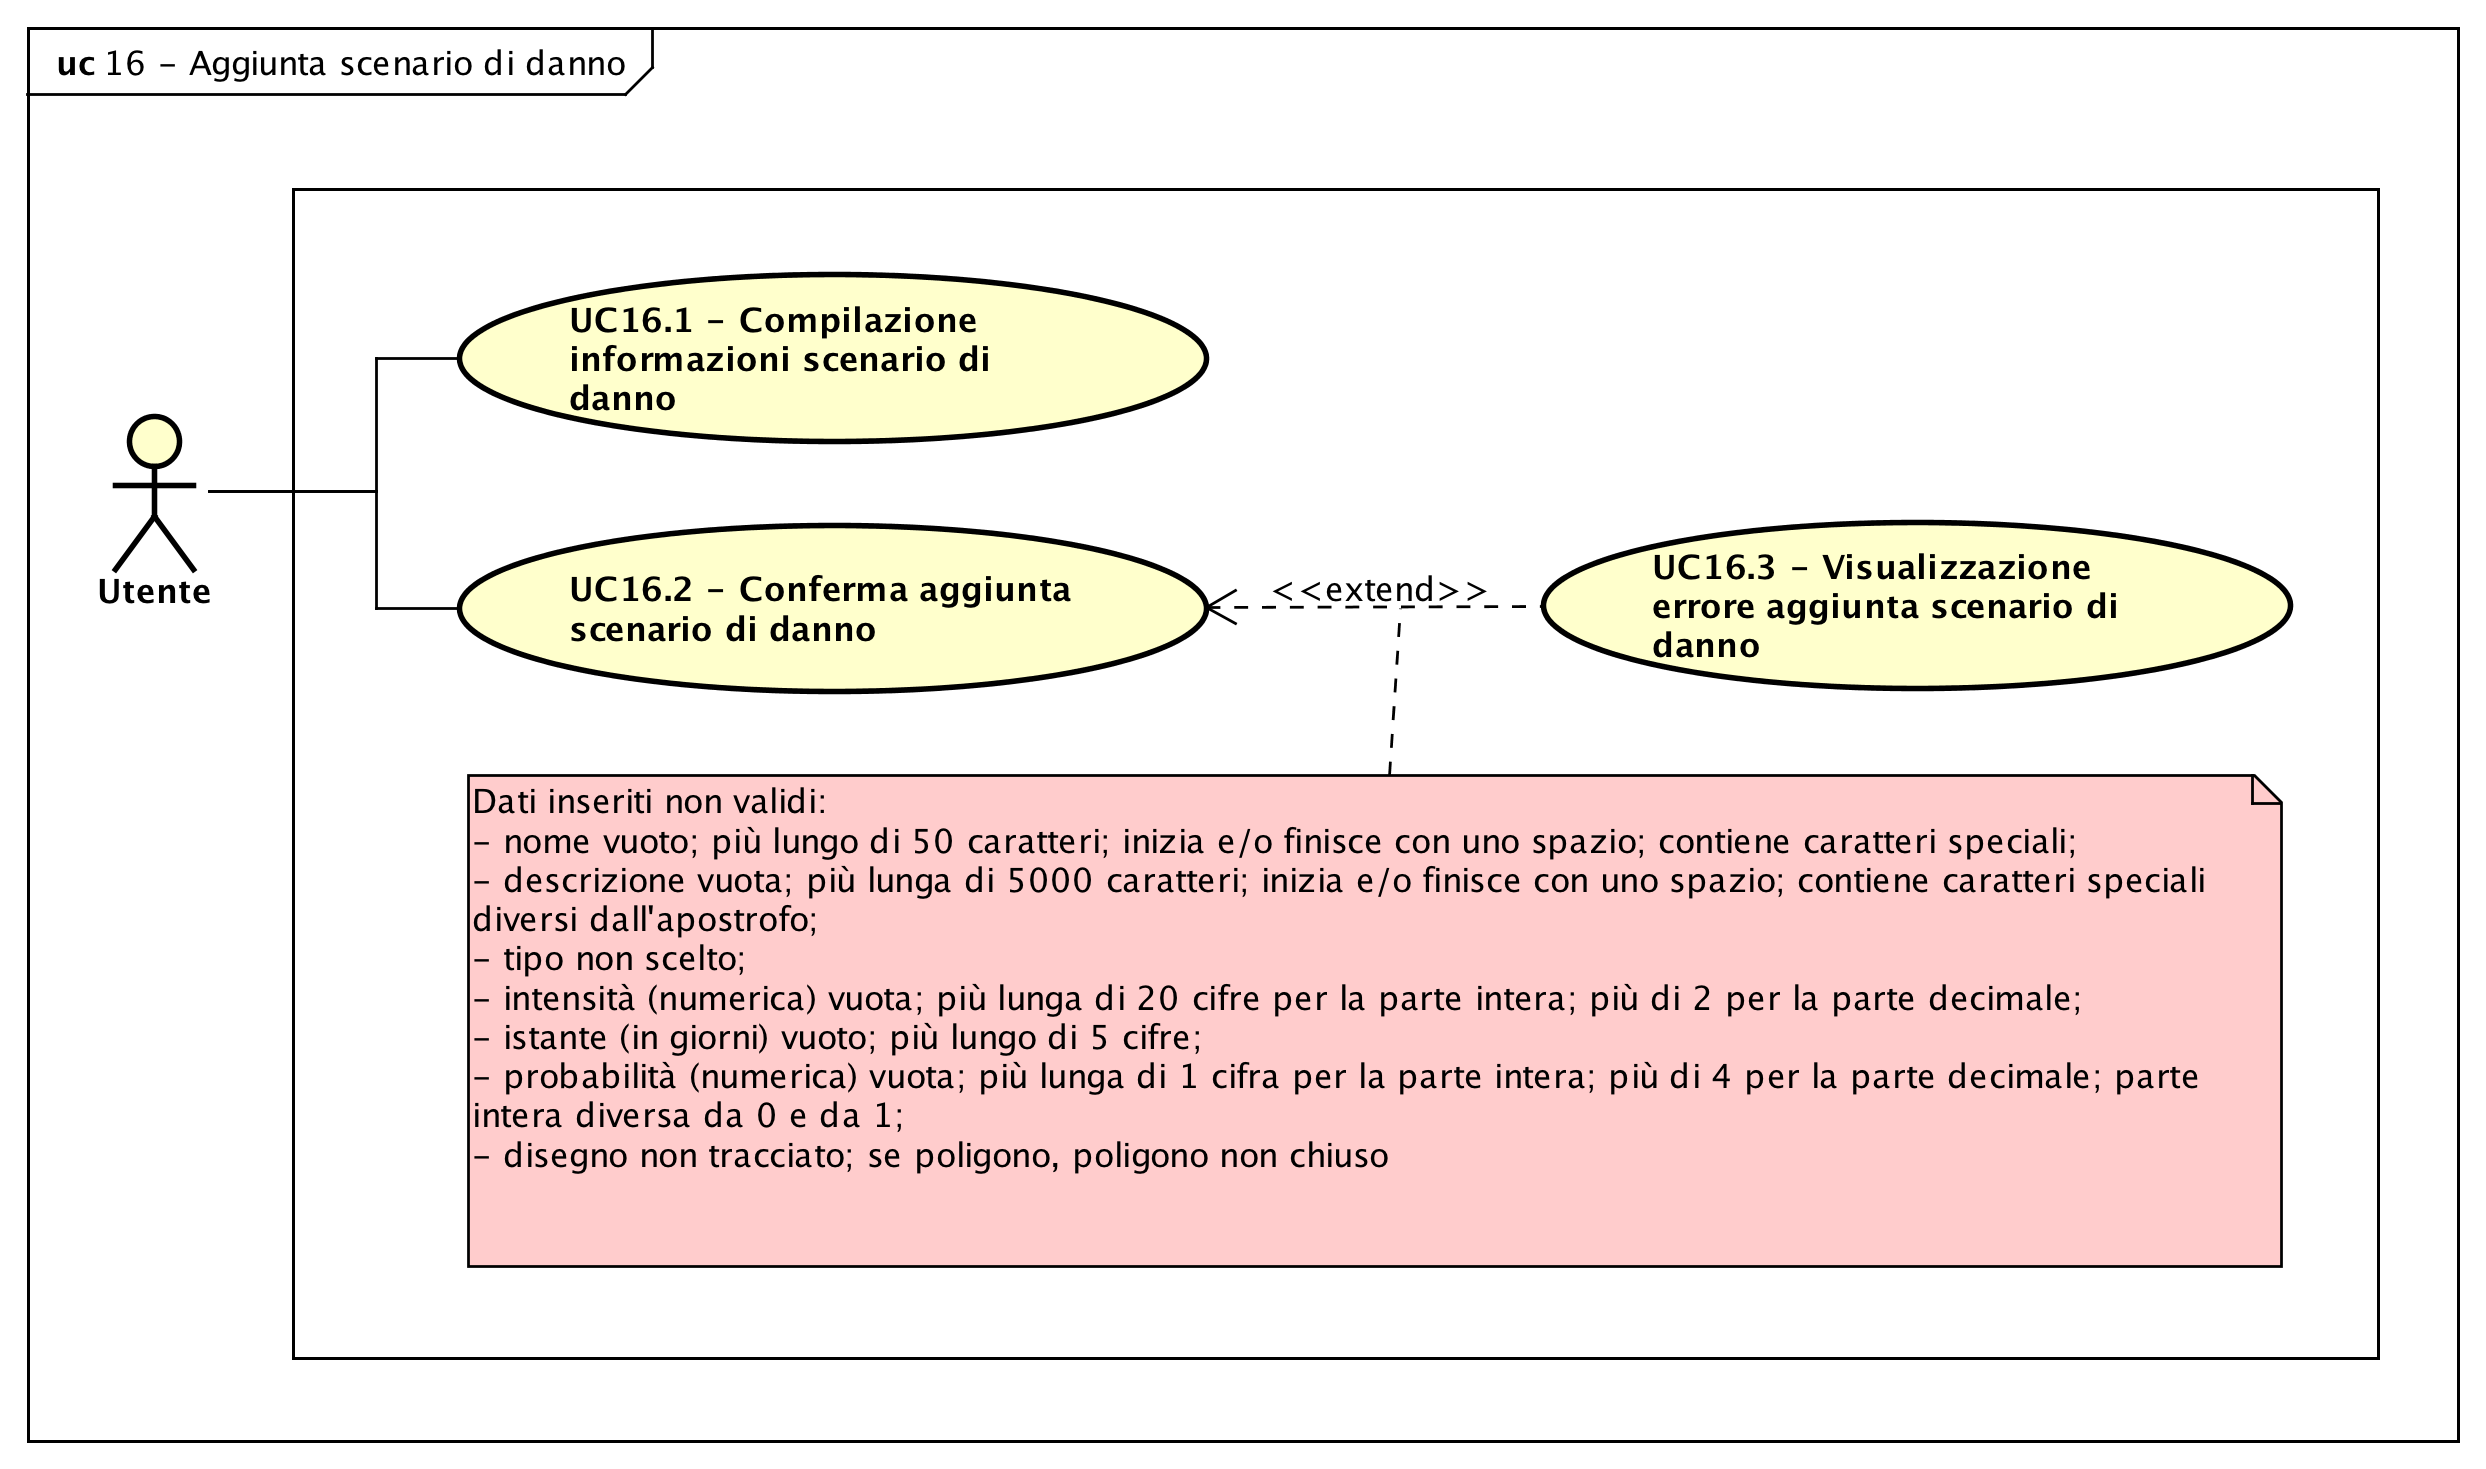
\includegraphics[width=\textwidth]{{img/uc16}.png} 
	\caption{UC16 - Aggiunta scenario di danno}
\end{figure}
\def\arraystretch{1.5}
\rowcolors{2}{D}{P}
\begin{tabularx}{\textwidth}{l|p{0.7\textwidth}}
	\rowcolor{I} \multicolumn{2}{c}{\color{white}\textbf{UC16 - Aggiunta scenario di danno}} \\
	\toprule
	\endhead
	\textbf{Attori} & Utente\\
	\textbf{Descrizione} & l'utente aggiunge uno scenario di danno\\
	\textbf{Pre-condizione} & l'utente ha aperto l'applicazione\\
	\textbf{Post-condizione} & un nuovo scenario di danno è stato aggiunto ed è visualizzabile sulla mappa; l'utente visualizza un messaggio che comunica la corretta esecuzione dell'operazione; l'area informativa rimane impostata sullo scenario appena inserito; la posizione e il livello di ingrandimento della mappa rimangono invariati\\
	\textbf{Scenario principale} & \vspace{-1.2em}\begin{enumerate}[leftmargin=*,noitemsep,nosep]
		\item \nameref{sssec:UC16.1};
		\item \nameref{sssec:UC16.2}.
	\end{enumerate}\\
	\textbf{Estensioni} & \vspace{-1.2em}\begin{itemize}[leftmargin=*,noitemsep,nosep]
		\item \nameref{sssec:UC39}: l’utente interrompe volontariamente l’aggiunta dello
		scenario di danno;
	\end{itemize}\\
	\textbf{Scenari alternativi} & \vspace{-1.2em}\begin{itemize}[leftmargin=*,noitemsep,nosep]
		\item \nameref{sssec:UC16.3}.
	\end{itemize}\\
	%\textbf{Generalizzazioni} &  \\
	\bottomrule
\end{tabularx}
\subsection{UC16.1 - Compilazione informazioni scenario di danno} 
\label{sssec:UC16.1} 
\begin{figure}[H] 
	\centering 
	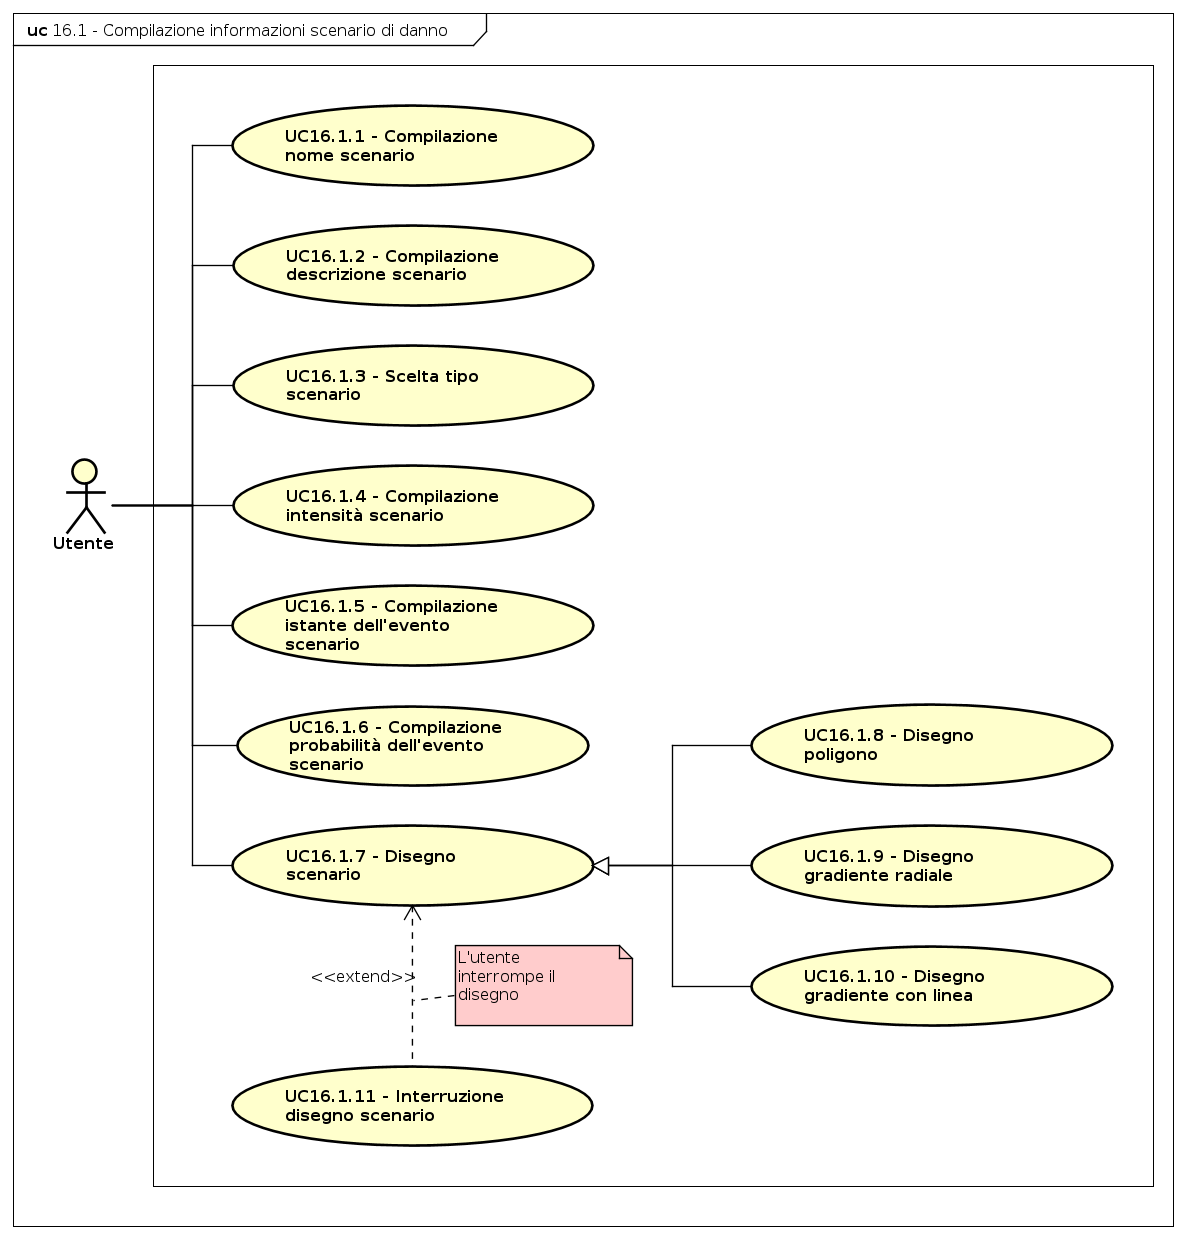
\includegraphics[width=\textwidth]{{img/uc16.1}.png} 
	\caption{UC16.1 - Compilazione informazioni scenario di danno}
\end{figure}
\def\arraystretch{1.5}
\rowcolors{2}{D}{P}
\begin{tabularx}{\textwidth}{l|p{0.7\textwidth}}
	\rowcolor{I} \multicolumn{2}{c}{\color{white}\textbf{UC16.1 - Compilazione informazioni scenario di danno}} \\
	\toprule
	\endhead
	\textbf{Attori} & Utente\\
	\textbf{Descrizione} & l'utente compila le informazioni dello scenario di danno\\
	\textbf{Pre-condizione} & il sistema offre la possbilità di compilare le informazioni dello scenario di danno\\
	\textbf{Post-condizione} & le informazioni dello scenario di danno sono state compilate e sono visualizzabili nell'area informativa; l'utente viene riportato alla schermata di aggiunta scenario, dove può confermarne l'aggiunta\\
	\textbf{Scenario principale} & \vspace{-1.2em}\begin{enumerate}[leftmargin=*,noitemsep,nosep]
		\item \nameref{sssec:UC16.1.1};
		\item \nameref{sssec:UC16.1.2};
		\item \nameref{sssec:UC16.1.3};
		\item \nameref{sssec:UC16.1.4};
		\item \nameref{sssec:UC16.1.5};
		\item \nameref{sssec:UC16.1.6};
		\item \nameref{sssec:UC16.1.8} oppure
		\item \nameref{sssec:UC16.1.9} oppure
		\item \nameref{sssec:UC16.1.10}.
	\end{enumerate}\\
	\textbf{Scenari alternativi} & \vspace{-1.2em}\begin{itemize}[leftmargin=*,noitemsep,nosep]
	\item \nameref{sssec:UC16.1.11}: : l’utente interrompe volontariamente il disegno dello
	scenario di danno
\end{itemize}\\
	%\textbf{Generalizzazioni} &  \\
	\bottomrule
\end{tabularx}
\subsection{UC16.1.1 - Compilazione nome scenario} 
\label{sssec:UC16.1.1} 
\def\arraystretch{1.5}
\rowcolors{2}{D}{P}
\begin{tabularx}{\textwidth}{l|p{0.7\textwidth}}
	\rowcolor{I} \multicolumn{2}{c}{\color{white}\textbf{UC16.1.1 - Compilazione nome scenario}} \\
	\toprule
	\endhead
	\textbf{Attori} & Utente\\
	\textbf{Descrizione} & l'utente compila il nome dello scenario\\
	\textbf{Pre-condizione} & il sistema offre la possibilità di compilare il nome dello scenario\\
	\textbf{Post-condizione} & l'utente ha compilato il nome dello scenario e può visualizzare il nome appena inserito nell'area informativa\\
	\textbf{Scenario principale} & \vspace{-1.2em}\begin{enumerate}[leftmargin=*,noitemsep,nosep]
		\item \nameref{sssec:UC16.1.1}.
	\end{enumerate}\\
	%\textbf{Generalizzazioni} &  \\
	\bottomrule
\end{tabularx}

\subsection{UC16.1.2 - Compilazione descrizione scenario} 
\label{sssec:UC16.1.2} 
\def\arraystretch{1.5}
\rowcolors{2}{D}{P}
\begin{tabularx}{\textwidth}{l|p{0.7\textwidth}}
	\rowcolor{I} \multicolumn{2}{c}{\color{white}\textbf{UC16.1.2 - Compilazione descrizione scenario}} \\
	\toprule
	\endhead
	\textbf{Attori} & Utente\\
	\textbf{Descrizione} & l'utente compila la descrizione dello scenario\\
	\textbf{Pre-condizione} & il sistema offre la possibilità di compilare la descrizione dello scenario\\
	\textbf{Post-condizione} & l'utente ha compilato la descrizione dello scenario e visualizza la descrizione appena compilata nell'area informativa\\
	\textbf{Scenario principale} & \vspace{-1.2em}\begin{enumerate}[leftmargin=*,noitemsep,nosep]
		\item \nameref{sssec:UC16.1.2}.
	\end{enumerate}\\
	%\textbf{Generalizzazioni} &  \\
	\bottomrule
\end{tabularx}
\subsection{UC16.1.3 - Scelta tipo scenario} 
\label{sssec:UC16.1.3} 
\def\arraystretch{1.5}
\rowcolors{2}{D}{P}
\begin{tabularx}{\textwidth}{l|p{0.7\textwidth}}
	\rowcolor{I} \multicolumn{2}{c}{\color{white}\textbf{UC16.1.3 - Scelta tipo scenario}} \\
	\toprule
	\endhead
	\textbf{Attori} & Utente\\
	\textbf{Descrizione} & l'utente sceglie il tipo di scenario\\
	\textbf{Pre-condizione} & il sistema offre la possibilità di scegliere il tipo di scenario\\
	\textbf{Post-condizione} & il tipo di scenario è stato scelto e l'utente visualizza il tipo appena scelto nell'area informativa\\
	\textbf{Scenario principale} & \vspace{-1.2em}\begin{enumerate}[leftmargin=*,noitemsep,nosep]
		\item \nameref{sssec:UC16.1.3}.
	\end{enumerate}\\
	%\textbf{Generalizzazioni} &  \\
	\bottomrule
\end{tabularx}
\subsection{UC16.1.4 - Compilazione intensità scenario} 
\label{sssec:UC16.1.4} 
\def\arraystretch{1.5}
\rowcolors{2}{D}{P}
\begin{tabularx}{\textwidth}{l|p{0.7\textwidth}}
	\rowcolor{I} \multicolumn{2}{c}{\color{white}\textbf{UC16.1.4 - Compilazione intensità scenario}} \\
	\toprule
	\endhead
	\textbf{Attori} & Utente\\
	\textbf{Descrizione} & l'utente compila l'intensità dello scenario\\
	\textbf{Pre-condizione} & il sistema offre la possibilità di compilare l'intensità dello scenario\\
	\textbf{Post-condizione} & l'utente ha compilato l'intensità dello scenario e visualizza l'intensità appena compilata nell'area informativa\\
	\textbf{Scenario principale} & \vspace{-1.2em}\begin{enumerate}[leftmargin=*,noitemsep,nosep]
		\item \nameref{sssec:UC16.1.4}.
	\end{enumerate}\\
	%\textbf{Generalizzazioni} &  \\
	\bottomrule
\end{tabularx}
\subsection{UC16.1.5 - Compilazione istante dell'evento scenario} 
\label{sssec:UC16.1.5} 
\def\arraystretch{1.5}
\rowcolors{2}{D}{P}
\begin{tabularx}{\textwidth}{l|p{0.7\textwidth}}
	\rowcolor{I} \multicolumn{2}{c}{\color{white}\textbf{UC16.1.5 - Compilazione istante dell'evento scenario}} \\
	\toprule
	\endhead
	\textbf{Attori} & Utente\\
	\textbf{Descrizione} & l'utente compila l'istante dell'evento dello scenario\\
	\textbf{Pre-condizione} & il sistema offre la possibilità di compilare l'istante dell'evento dello scenario\\
	\textbf{Post-condizione} & l'istante dell'evento dello scenario è stato compilato e l'utente visualizza l'istante appena compilato nell'area informativa\\
	\textbf{Scenario principale} & \vspace{-1.2em}\begin{enumerate}[leftmargin=*,noitemsep,nosep]
		\item \nameref{sssec:UC16.1.5}.
	\end{enumerate}\\
	%\textbf{Generalizzazioni} &  \\
	\bottomrule
\end{tabularx}
\subsection{UC16.1.6 - Compilazione probabilità dell'evento scenario} 
\label{sssec:UC16.1.6} 
\def\arraystretch{1.5}
\rowcolors{2}{D}{P}
\begin{tabularx}{\textwidth}{l|p{0.7\textwidth}}
	\rowcolor{I} \multicolumn{2}{c}{\color{white}\textbf{UC16.1.6 - Compilazione probabilità dell'evento scenario}} \\
	\toprule
	\endhead
	\textbf{Attori} & Utente\\
	\textbf{Descrizione} & l'utente compila la probabilità dell'evento dello scenario\\
	\textbf{Pre-condizione} & il sistema offre la possibilità di compilare la probabilità dell'evento dello scenario\\
	\textbf{Post-condizione} & la probabilità dell'evento dello scenario è stata compilata e l'utente visualizza la probabilità appena compilata nell'area informativa\\
	\textbf{Scenario principale} & \vspace{-1.2em}\begin{enumerate}[leftmargin=*,noitemsep,nosep]
		\item \nameref{sssec:UC16.1.6}.
	\end{enumerate}\\
	%\textbf{Generalizzazioni} &  \\
	\bottomrule
\end{tabularx}
	\subsection{UC16.1.7 - Disegno scenario} 
\label{sssec:UC16.1.7} 
\def\arraystretch{1.5}
\rowcolors{2}{D}{P}
\begin{tabularx}{\textwidth}{l|p{0.7\textwidth}}
	\rowcolor{I} \multicolumn{2}{c}{\color{white}\textbf{UC16.1.7 - Disegno scenario}} \\
	\toprule
	\endhead
	\textbf{Attori} & Utente\\
	\textbf{Descrizione} & l'utente disegna lo scenario di danno\\
	\textbf{Pre-condizione} & il sistema offre la possibilità di disegnare lo scenario di danno\\
	\textbf{Post-condizione} & lo scenario di danno è stato disegnato e viene visualizzato sulla mappa\\
	\textbf{Scenario principale} & \vspace{-1.2em}\begin{enumerate}[leftmargin=*,noitemsep,nosep]
		\item \nameref{sssec:UC16.1.7}.
	\end{enumerate}\\
	\textbf{Estensioni} & \vspace{-1.2em}\begin{itemize}[leftmargin=*,noitemsep,nosep]
		\item \nameref{sssec:UC16.1.11}: l’utente interrompe volontariamente il disegno dello
		scenario di danno
	\end{itemize}\\
	\textbf{Generalizzazioni} &
	\vspace{-1.2em}\begin{itemize}
		[leftmargin=*,noitemsep,nosep]
		\item \nameref{sssec:UC16.1.8};
		\item \nameref{sssec:UC16.1.9};
		\item \nameref{sssec:UC16.1.10};
	\end{itemize} \\
	
	\bottomrule
\end{tabularx}
\subsection{UC16.1.8 - Disegno poligono} 
\label{sssec:UC16.1.8} 
\def\arraystretch{1.5}
\rowcolors{2}{D}{P}
\begin{tabularx}{\textwidth}{l|p{0.7\textwidth}}
	\rowcolor{I} \multicolumn{2}{c}{\color{white}\textbf{UC16.1.8 - Disegno poligono}} \\
	\toprule
	\endhead
	\textbf{Attori} & Utente\\
	\textbf{Descrizione} & l'utente disegna lo scenario mediante poligono\\
	\textbf{Pre-condizione} & il sistema offre la possibilità di disegnare lo scenario\\
	\textbf{Post-condizione} & lo scenario è stato disegnato mediante poligono e viene visualizzato sulla mappa\\
	\textbf{Scenario principale} & \vspace{-1.2em}\begin{enumerate}[leftmargin=*,noitemsep,nosep]
		\item \nameref{sssec:UC16.1.8}.
	\end{enumerate}\\
	%\textbf{Generalizzazioni} &  \\
	\bottomrule
\end{tabularx}
\subsection{UC16.1.9 - Disegno gradiente radiale} 
\label{sssec:UC16.1.9} 
\def\arraystretch{1.5}
\rowcolors{2}{D}{P}
\begin{tabularx}{\textwidth}{l|p{0.7\textwidth}}
	\rowcolor{I} \multicolumn{2}{c}{\color{white}\textbf{UC16.1.9 - Disegno gradiente radiale}} \\
	\toprule
	\endhead
	\textbf{Attori} & Utente\\
	\textbf{Descrizione} & l'utente disegna lo scenario di danno mediante gradiente radiale\\
	\textbf{Pre-condizione} & il sistema offre la possibilità di disegnare lo scenario\\
	\textbf{Post-condizione} & lo scenario è stato disegnato mediante gradiente radiale e viene visualizzato sulla mappa\\
	\textbf{Scenario principale} & \vspace{-1.2em}\begin{enumerate}[leftmargin=*,noitemsep,nosep]
		\item \nameref{sssec:UC16.1.9}.
	\end{enumerate}\\
	%\textbf{Generalizzazioni} &  \\
	\bottomrule
\end{tabularx}
\subsection{UC16.1.10 - Disegno gradiente con linea} 
\label{sssec:UC16.1.10} 
\def\arraystretch{1.5}
\rowcolors{2}{D}{P}
\begin{tabularx}{\textwidth}{l|p{0.7\textwidth}}
	\rowcolor{I} \multicolumn{2}{c}{\color{white}\textbf{UC16.1.10 - Disegno gradiente con linea}} \\
	\toprule
	\endhead
	\textbf{Attori} & Utente\\
	\textbf{Descrizione} & l'utente disegna lo scenario di danno mediante gradiente con linea\\
	\textbf{Pre-condizione} & il sistema offre la possibilità di disegnare lo scenario\\
	\textbf{Post-condizione} & lo scenario è stato disegnato mediante gradiente con linea; l'utente può visualizzare il gradiente sulla mappa\\
	\textbf{Scenario principale} & \vspace{-1.2em}\begin{enumerate}[leftmargin=*,noitemsep,nosep]
		\item \nameref{sssec:UC16.1.10}.
	\end{enumerate}\\
	%\textbf{Generalizzazioni} &  \\
	\bottomrule
\end{tabularx}
\subsection{UC16.1.11 - Interruzione disegno scenario} 
\label{sssec:UC16.1.11} 
\def\arraystretch{1.5}
\rowcolors{2}{D}{P}
\begin{tabularx}{\textwidth}{l|p{0.7\textwidth}}
	\rowcolor{I} \multicolumn{2}{c}{\color{white}\textbf{UC16.1.11 - Interruzione disegno scenario}} \\
	\toprule
	\endhead
	\textbf{Attori} & Utente\\
	\textbf{Descrizione} & l'utente interrompe il disegno dello scenario\\
	\textbf{Pre-condizione} & il sistema offre la possibilità di disegnare lo scenario\\
	\textbf{Post-condizione} & lo scenario non è stato disegnato; l'utente viene riportato alla schermata di inserimento scenario\\
	\textbf{Scenario principale} & \vspace{-1.2em}\begin{enumerate}[leftmargin=*,noitemsep,nosep]
		\item \nameref{sssec:UC16.1.11}.
	\end{enumerate}\\
	%\textbf{Generalizzazioni} &  \\
	\bottomrule
\end{tabularx}
\subsection{UC16.2 - Conferma aggiunta scenario di danno} 
\label{sssec:UC16.2} 
\def\arraystretch{1.5}
\rowcolors{2}{D}{P}
\begin{tabularx}{\textwidth}{l|p{0.7\textwidth}}
	\rowcolor{I} \multicolumn{2}{c}{\color{white}\textbf{UC16.2 - Conferma aggiunta scenario di danno}} \\
	\toprule
	\endhead
	\textbf{Attori} & Utente\\
	\textbf{Descrizione} & l'utente conferma l'aggiunta dello scenario di danno\\
	\textbf{Pre-condizione} & il sistema offre la possibilità di confermare l'aggiunta dello scenario di danno\\
	\textbf{Post-condizione} & un nuovo scenario di danno è stato aggiunto ma non viene visualizzato sulla mappa; l'utente visualizza un messaggio che comunica la corretta esecuzione dell'operazione; l'area informativa viene impostata alla visualizzazione di default; la posizione e il livello di ingrandimento della mappa rimangono invariati\\
	\textbf{Scenario principale} & \vspace{-1.2em}\begin{enumerate}[leftmargin=*,noitemsep,nosep]
		\item \nameref{sssec:UC16.2}.
	\end{enumerate}\\
	\textbf{Estensioni} & \vspace{-1.2em}\begin{itemize}[leftmargin=*,noitemsep,nosep]
		\item \nameref{sssec:UC16.3}: dati inseriti non validi:
		\begin{itemize}
			\item nome vuoto; più lungo di 50 caratteri; inizia e/o
			finisce con uno spazio; contiene caratteri speciali;
			\item descrizione vuota; più lunga di 5000 caratteri;
			inizia e/o finisce con uno spazio; contiene
			caratteri speciali diversi dall'apostrofo;
			\item tipo non scelto;
			\item intensità (numerica) vuota; più lunga di 20 cifre per la
			parte intera; più di 2 per la parte decimale;
			\item istante (in giorni) vuoto; più lungo di 5 cifre;
			\item probabilità (numerica) vuota; più lunga di 1 cifra per la
			parte intera; più di 4 per la parte decimale; parte
			intera diversa da 0 e da 1;
			\item disegno non tracciato; se poligono, poligono non
			chiuso
		\end{itemize}
	\end{itemize}\\
	%\textbf{Generalizzazioni} &  \\
	\bottomrule
\end{tabularx}
\subsection{UC16.3 - Visualizzazione errore aggiunta scenario di danno} 
\label{sssec:UC16.3} 
\def\arraystretch{1.5}
\rowcolors{2}{D}{P}
\begin{tabularx}{\textwidth}{l|p{0.7\textwidth}}
	\rowcolor{I} \multicolumn{2}{c}{\color{white}\textbf{UC16.3 - Visualizzazione errore aggiunta scenario di danno}} \\
	\toprule
	\endhead
	\textbf{Attori} & Utente\\
	\textbf{Descrizione} & l'utente visualizza un errore relativo ai dati dello scenario di danno compilati in modo errato\\
	\textbf{Pre-condizione} & l'utente sta tentando di inserire un nuovo scenario di danno\\
	\textbf{Post-condizione} & nessun nuovo scenario di danno inserito;  l'utente visualizza un errore relativo ai dati dello scenario di danno compilati in modo errato; l'utente viene riportato alla schermata di aggiunta scenario\\
	\textbf{Scenario principale} & \vspace{-1.2em}\begin{enumerate}[leftmargin=*,noitemsep,nosep]
		\item \nameref{sssec:UC16.3}.
	\end{enumerate}\\
	%\textbf{Generalizzazioni} &  \\
	\bottomrule
\end{tabularx}
\subsection{UC17 - Scelta visualizzazione scenario di danno} 
\label{sssec:UC17} 
\def\arraystretch{1.5}
\rowcolors{2}{D}{P}
\begin{tabularx}{\textwidth}{l|p{0.7\textwidth}}
	\rowcolor{I} \multicolumn{2}{c}{\color{white}\textbf{UC17 - Scelta visualizzazione scenario di danno}} \\
	\toprule
	\endhead
	\textbf{Attori} & Utente\\
	\textbf{Descrizione} & l'utente sceglie quale scenario di danno visualizzare\\
	\textbf{Pre-condizione} & l'utente ha aperto l'applicazione; almeno uno scenario di danno è stato inserito\\
	\textbf{Post-condizione} & il sistema mostra nell'area informativa le informazioni dello scenario di danno selezionato; la posizione e il livello di ingrandimento della mappa rimangono invariati\\
	\textbf{Scenario principale} & \vspace{-1.2em}\begin{enumerate}[leftmargin=*,noitemsep,nosep]
		\item \nameref{sssec:UC17}.
	\end{enumerate}\\
	%\textbf{Generalizzazioni} &  \\
	\bottomrule
\end{tabularx}
\subsection{UC18 - Chiusura visualizzazione scenario di danno} 
\label{sssec:UC18} 
\def\arraystretch{1.5}
\rowcolors{2}{D}{P}
\begin{tabularx}{\textwidth}{l|p{0.7\textwidth}}
	\rowcolor{I} \multicolumn{2}{c}{\color{white}\textbf{UC18 - Chiusura visualizzazione scenario di danno}} \\
	\toprule
	\endhead
	\textbf{Attori} & Utente\\
	\textbf{Descrizione} & l'utente chiude la visualizzazione dello scenario di danno\\
	\textbf{Pre-condizione} & l'utente ha aperto l'applicazione; uno scenario di danno è visualizzato sulla mappa\\
	\textbf{Post-condizione} & è stata chiusa la visualizzazione delle informazioni dello scenario di danno selezionato nell'area informativa; l'area informativa viene impostata sulla visualizzazione di default; la posizione e il livello di ingrandimento della mappa rimangono invariati\\
	\textbf{Scenario principale} & \vspace{-1.2em}\begin{enumerate}[leftmargin=*,noitemsep,nosep]
		\item \nameref{sssec:UC18}.
	\end{enumerate}\\
	%\textbf{Generalizzazioni} &  \\
	\bottomrule
\end{tabularx}
\subsection{UC19 - Modifica scenario di danno} 
\label{sssec:UC19} 
\begin{figure}[H] 
	\centering 
	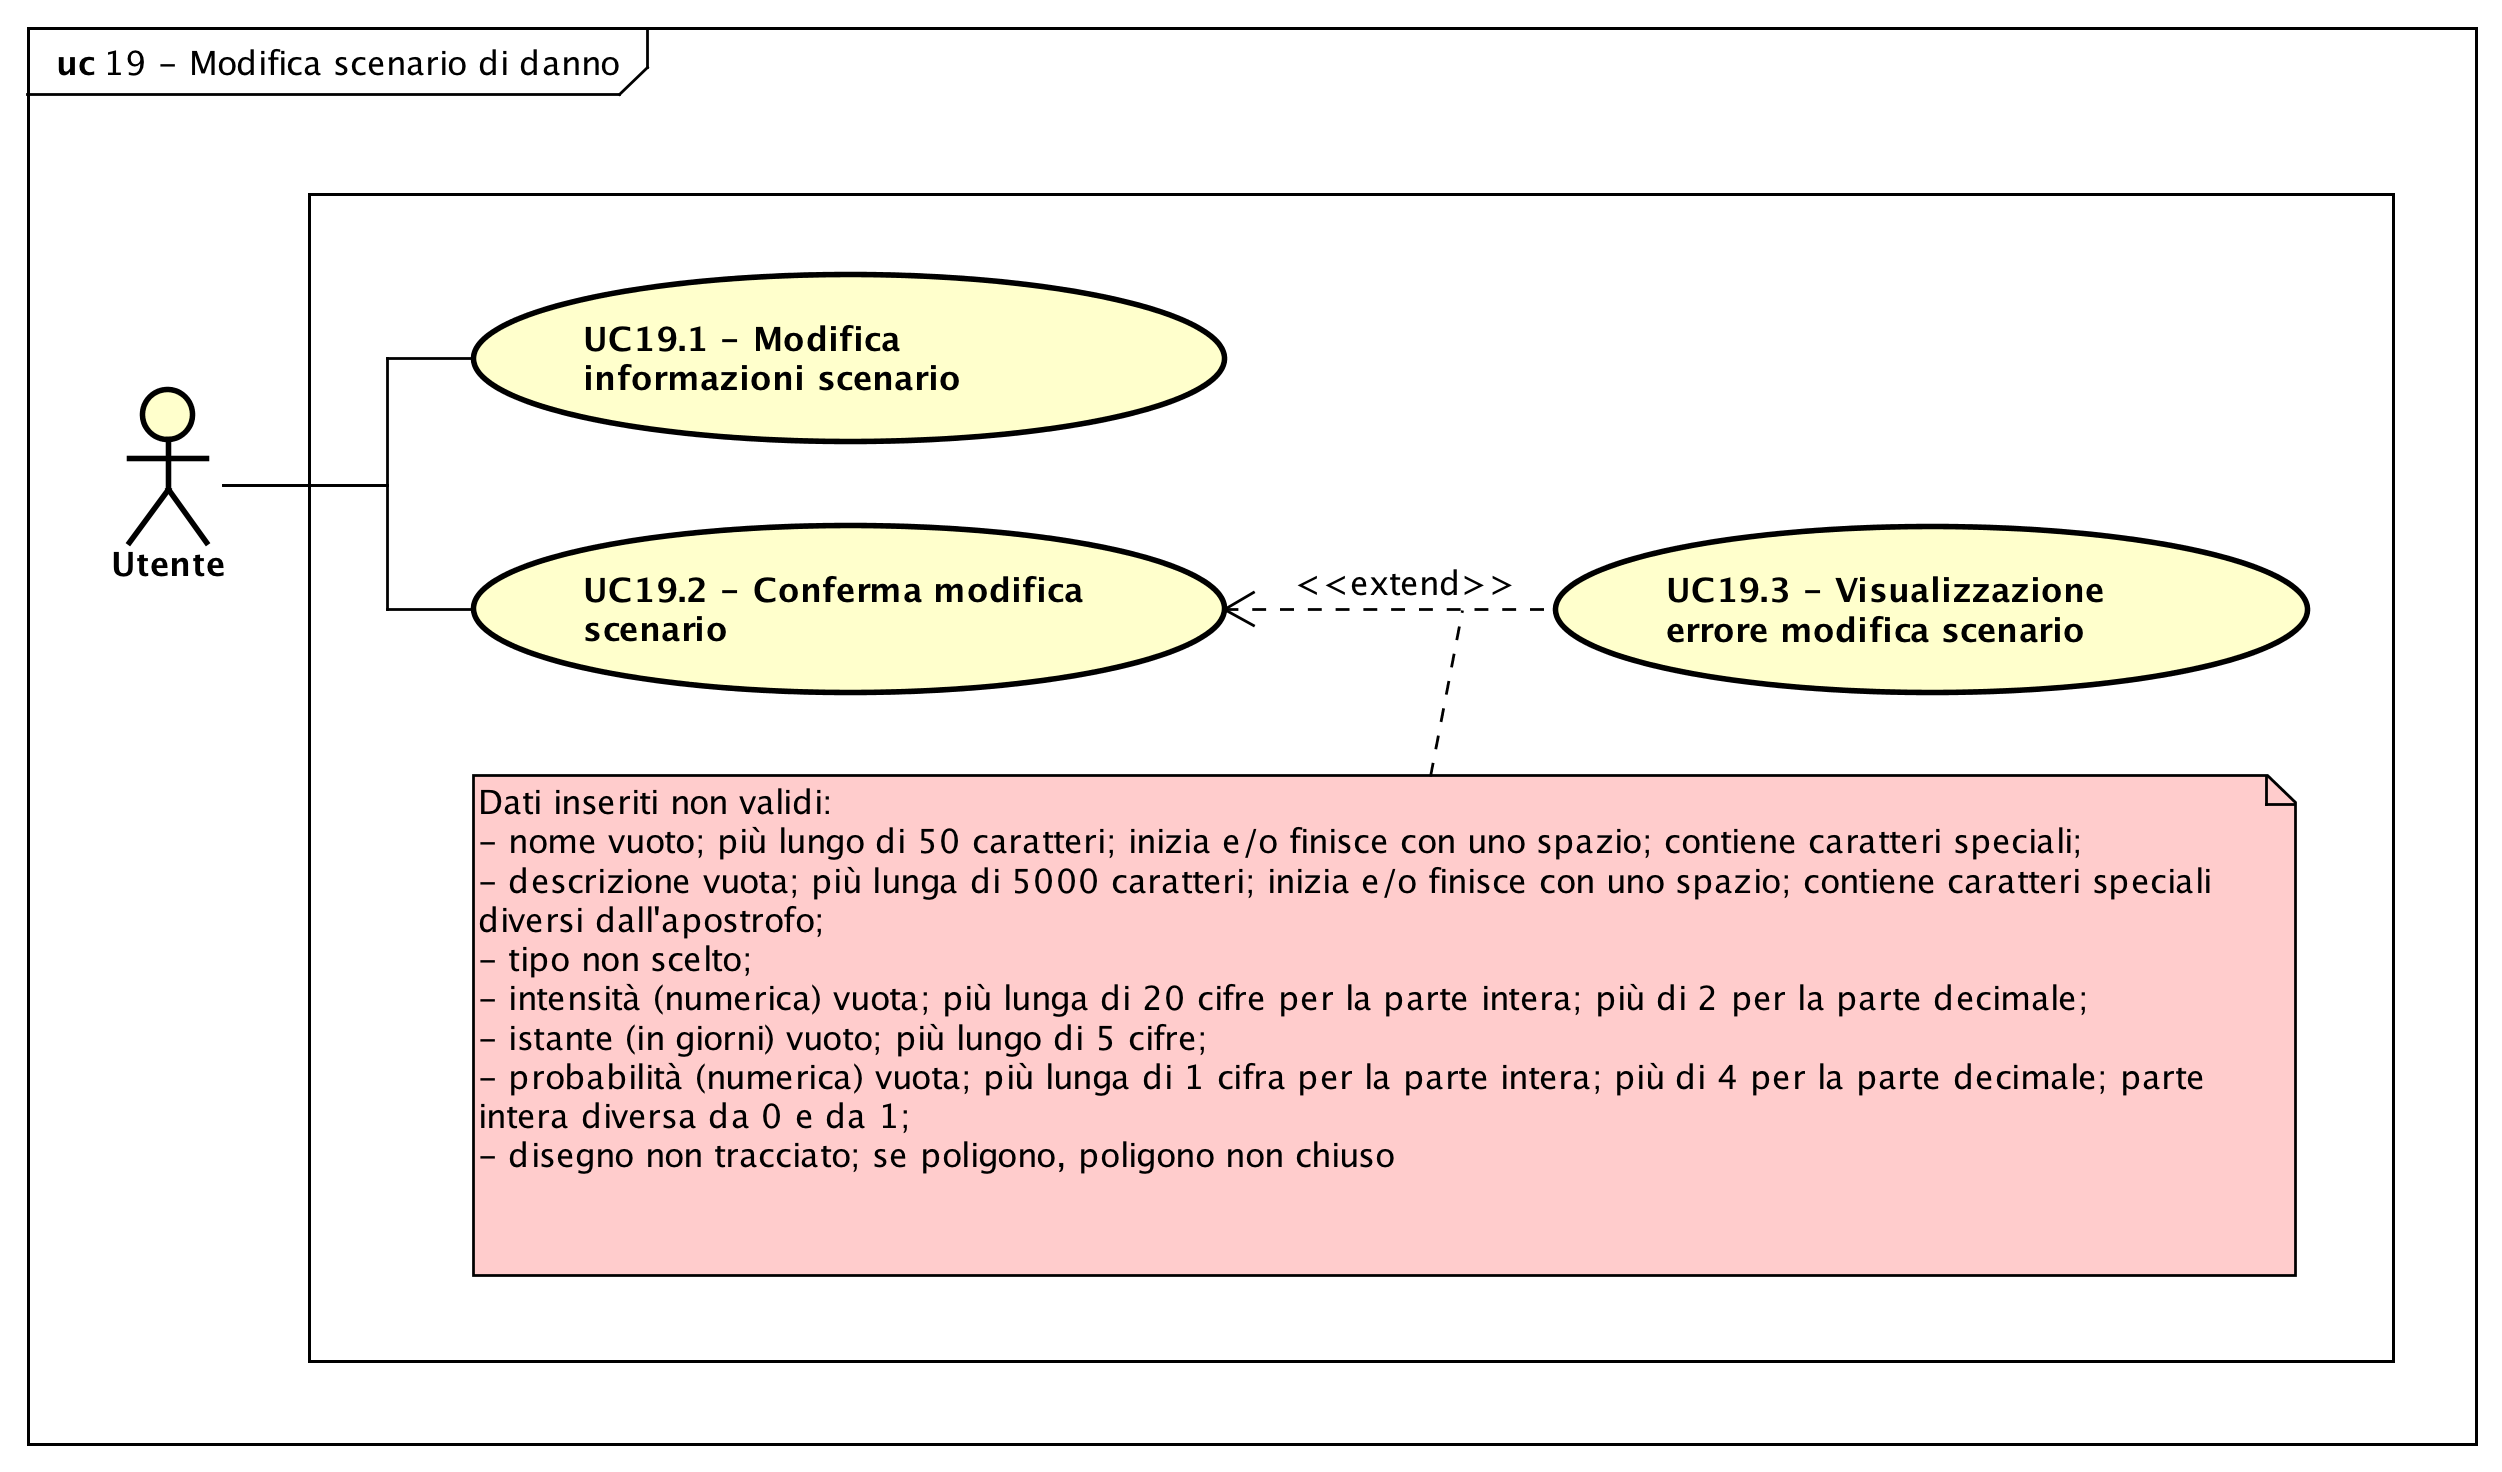
\includegraphics[width=\textwidth]{{img/uc19}.png} 
	\caption{UC19 - Modifica scenario di danno}
\end{figure}
\def\arraystretch{1.5}
\rowcolors{2}{D}{P}
\begin{tabularx}{\textwidth}{l|p{0.7\textwidth}}
	\rowcolor{I} \multicolumn{2}{c}{\color{white}\textbf{UC19 - Modifica scenario di danno}} \\
	\toprule
	\endhead
	\textbf{Attori} & Utente\\
	\textbf{Descrizione} & l'utente modifica lo scenario di danno\\
	\textbf{Pre-condizione} & l'utente ha aperto l'applicazione; almeno uno scenario di danno è stato aggiunto; l'utente ha selezionato uno scenario di danno\\
	\textbf{Post-condizione} & lo scenario di danno è stato modificato; l'utente viisualizza un messaggio che comunica la corretta esecuzione dell'operazione; l'area informativa rimane impostata sullo scenario appena modificato; la posizione e il livello di ingrandimento della mappa rimangono invariati\\
	\textbf{Scenario principale} & \vspace{-1.2em}\begin{enumerate}[leftmargin=*,noitemsep,nosep]
		\item \nameref{sssec:UC19.1};
		\item \nameref{sssec:UC19.2}.
	\end{enumerate}\\
	\textbf{Estensioni} & \vspace{-1.2em}\begin{itemize}[leftmargin=*,noitemsep,nosep]
		\item \nameref{sssec:UC40}: l’utente interrompe volontariamente la modifica dello
		scenario di danno
	\end{itemize}\\
	\textbf{Scenari alternativi} & \vspace{-1.2em}\begin{itemize}[leftmargin=*,noitemsep,nosep]
		\item \nameref{sssec:UC19.3}.
	\end{itemize}\\
	%\textbf{Generalizzazioni} &  \\
	\bottomrule
\end{tabularx}
\subsection{UC19.1 - Modifica informazioni scenario} 
\label{sssec:UC19.1} 
\begin{figure}[H] 
	\centering 
	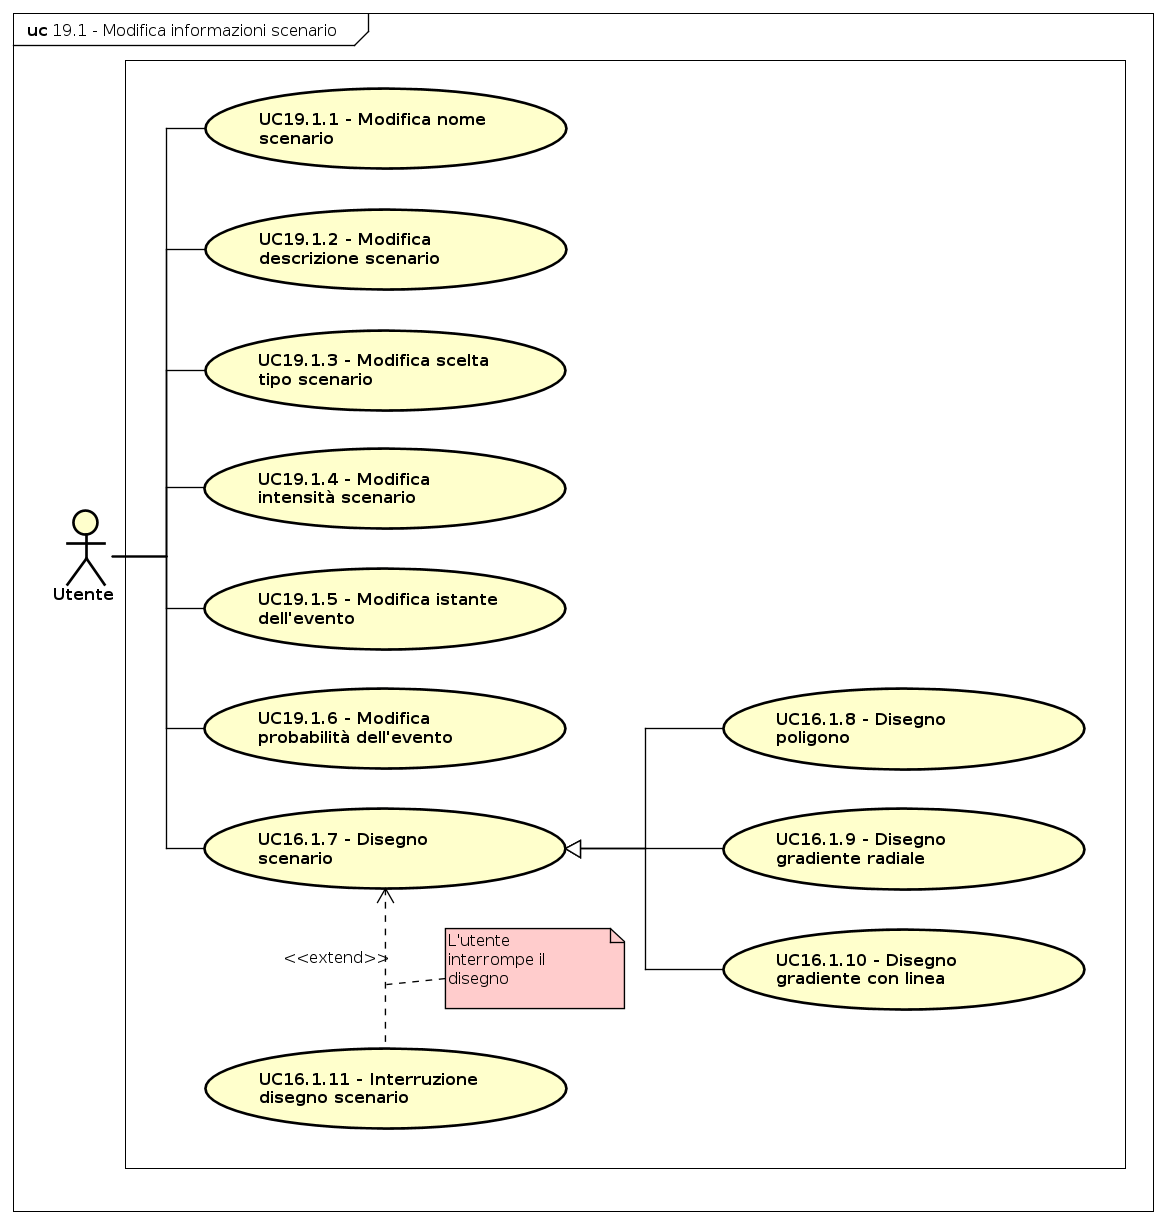
\includegraphics[width=\textwidth]{{img/uc19.1}.png} 
	\caption{UC4 - Modifica informazioni scenario}
\end{figure}
\def\arraystretch{1.5}
\rowcolors{2}{D}{P}
\begin{tabularx}{\textwidth}{l|p{0.7\textwidth}}
	\rowcolor{I} \multicolumn{2}{c}{\color{white}\textbf{UC19.1 - Modifica informazioni scenario}} \\
	\toprule
	\endhead
	\textbf{Attori} & Utente\\
	\textbf{Descrizione} & l'utente modifica le informazioni dello scenario\\
	\textbf{Pre-condizione} & il sistema offre la possibilità di modificare le informazioni dello scenario\\
	\textbf{Post-condizione} & le informazioni dello scenario sono state modificate; l'utente viene riportato alla schermata di modifica scenario, dove può confermare la modifica\\
	\textbf{Scenario principale} & \vspace{-1.2em}\begin{enumerate}[leftmargin=*,noitemsep,nosep]
		\item \nameref{sssec:UC19.1.1};
		\item \nameref{sssec:UC19.1.2};
		\item \nameref{sssec:UC19.1.3};
		\item \nameref{sssec:UC19.1.4};
		\item \nameref{sssec:UC19.1.5};
		\item \nameref{sssec:UC19.1.6};
		\item \nameref{sssec:UC16.1.8} oppure
		\item \nameref{sssec:UC16.1.9} oppure
		\item \nameref{sssec:UC16.1.10}.
	\end{enumerate}\\
\textbf{Scenari alternativi} & \vspace{-1.2em}\begin{itemize}[leftmargin=*,noitemsep,nosep]
	\item \nameref{sssec:UC16.1.11}: : l’utente interrompe volontariamente il disegno dello
	scenario di danno
\end{itemize}\\
	%\textbf{Generalizzazioni} &  \\
	\bottomrule
\end{tabularx}
\subsection{UC19.1.1 - Modifica nome scenario} 
\label{sssec:UC19.1.1} 
\def\arraystretch{1.5}
\rowcolors{2}{D}{P}
\begin{tabularx}{\textwidth}{l|p{0.7\textwidth}}
	\rowcolor{I} \multicolumn{2}{c}{\color{white}\textbf{UC19.1.1 - Modifica nome scenario}} \\
	\toprule
	\endhead
	\textbf{Attori} & Utente\\
	\textbf{Descrizione} & l'utente modifica il campo relativo al nome dello scenario\\
	\textbf{Pre-condizione} & il sistema offre la possibilità di modificare il nome dello scenario\\
	\textbf{Post-condizione} & il campo relativo al nome dello scenario è stato modificato; l'utente visualizza il nome appena inserito nell'area informativa\\
	\textbf{Scenario principale} & \vspace{-1.2em}\begin{enumerate}[leftmargin=*,noitemsep,nosep]
		\item \nameref{sssec:UC19.1.1}.
	\end{enumerate}\\
	%\textbf{Generalizzazioni} &  \\
	\bottomrule
\end{tabularx}
\subsection{UC19.1.2 - Modifica descrizione scenario} 
\label{sssec:UC19.1.2} 
\def\arraystretch{1.5}
\rowcolors{2}{D}{P}
\begin{tabularx}{\textwidth}{l|p{0.7\textwidth}}
	\rowcolor{I} \multicolumn{2}{c}{\color{white}\textbf{UC19.1.2 - Modifica descrizione scenario}} \\
	\toprule
	\endhead
	\textbf{Attori} & Utente\\
	\textbf{Descrizione} & l'utente modifica il campo relativo alla descrizione dello scenario\\
	\textbf{Pre-condizione} & il sistema offre la possibilità di modifica la descrizione dello scenario\\
	\textbf{Post-condizione} & il campo relativo alla descrizione dello scenario  è stato modificato; l'utente visualizza la descrizione appena inserita nell'area informativa\\
	\textbf{Scenario principale} & \vspace{-1.2em}\begin{enumerate}[leftmargin=*,noitemsep,nosep]
		\item \nameref{sssec:UC19.1.2}.
	\end{enumerate}\\
	%\textbf{Generalizzazioni} &  \\
	\bottomrule
\end{tabularx}
\subsection{UC19.1.3 - Modifica scelta tipo scenario} 
\label{sssec:UC19.1.3} 
\def\arraystretch{1.5}
\rowcolors{2}{D}{P}
\begin{tabularx}{\textwidth}{l|p{0.7\textwidth}}
	\rowcolor{I} \multicolumn{2}{c}{\color{white}\textbf{UC19.1.3 - Modifica scelta tipo scenario}} \\
	\toprule
	\endhead
	\textbf{Attori} & Utente\\
	\textbf{Descrizione} & l'utente modifica la scelta del tipo di scenario\\
	\textbf{Pre-condizione} & il sistema offre la possibilità di modificare la scelta del tipo di scenario\\
	\textbf{Post-condizione} & la scelta relativa al tipo dello scenario è stata modificata; l'utente visualizza il tipo di scenario appena scelto nell'area informativa\\
	\textbf{Scenario principale} & \vspace{-1.2em}\begin{enumerate}[leftmargin=*,noitemsep,nosep]
		\item \nameref{sssec:UC19.1.3}.
	\end{enumerate}\\
	%\textbf{Generalizzazioni} &  \\
	\bottomrule
\end{tabularx}
\subsection{UC19.1.4 - Modifica intensità scenario} 
\label{sssec:UC19.1.4} 
\def\arraystretch{1.5}
\rowcolors{2}{D}{P}
\begin{tabularx}{\textwidth}{l|p{0.7\textwidth}}
	\rowcolor{I} \multicolumn{2}{c}{\color{white}\textbf{UC19.1.4 - Modifica intensità scenario}} \\
	\toprule
	\endhead
	\textbf{Attori} & Utente\\
	\textbf{Descrizione} & l'utente modifica il campo relativo all'intensità dello scenario\\
	\textbf{Pre-condizione} & il sistema offre la possibilità di modificare l'intensità dello scenario\\
	\textbf{Post-condizione} & il campo relativo  all'intensità è stato modificato e l'utente visualizza l'intensità appena compilata nell'area informativa\\
	\textbf{Scenario principale} & \vspace{-1.2em}\begin{enumerate}[leftmargin=*,noitemsep,nosep]
		\item \nameref{sssec:UC19.1.4}.
	\end{enumerate}\\
	%\textbf{Generalizzazioni} &  \\
	\bottomrule
\end{tabularx}
\subsection{UC19.1.5 - Modifica istante dell'evento} 
\label{sssec:UC19.1.5} 
\def\arraystretch{1.5}
\rowcolors{2}{D}{P}
\begin{tabularx}{\textwidth}{l|p{0.7\textwidth}}
	\rowcolor{I} \multicolumn{2}{c}{\color{white}\textbf{UC19.1.5 - Modifica istante dell'evento}} \\
	\toprule
	\endhead
	\textbf{Attori} & Utente\\
	\textbf{Descrizione} & l'utente modifica il campo relativo all'istante dell'evento\\
	\textbf{Pre-condizione} & il sistema offre la possibilità di modificare l'istante dell'evento dello scenario\\
	\textbf{Post-condizione} & il campo relativo al nome all'istante dell'evento dello scenario è stato modificato; l'utente visualizza l'istante appena compilato nell'area informativa\\
	\textbf{Scenario principale} & \vspace{-1.2em}\begin{enumerate}[leftmargin=*,noitemsep,nosep]
		\item \nameref{sssec:UC19.1.5}.
	\end{enumerate}\\
	%\textbf{Generalizzazioni} &  \\
	\bottomrule
\end{tabularx}
\subsection{UC19.1.6 - Modifica probabilità dell'evento} 
\label{sssec:UC19.1.6} 
\def\arraystretch{1.5}
\rowcolors{2}{D}{P}
\begin{tabularx}{\textwidth}{l|p{0.7\textwidth}}
	\rowcolor{I} \multicolumn{2}{c}{\color{white}\textbf{UC19.1.6 - Modifica probabilità dell'evento}} \\
	\toprule
	\endhead
	\textbf{Attori} & Utente\\
	\textbf{Descrizione} & l'utente modifica la probabilità dell'evento dello scenario\\
	\textbf{Pre-condizione} & il sistema offre la possibilità di modificare la probabilità dell'evento dello scenario\\
	\textbf{Post-condizione} & la probabilità dell'evento dello scenario è stata modificata; l'utente visualizza la probabilità appena compilata nell'area informativa\\
	\textbf{Scenario principale} & \vspace{-1.2em}\begin{enumerate}[leftmargin=*,noitemsep,nosep]
		\item \nameref{sssec:UC19.1.6}.
	\end{enumerate}\\
	%\textbf{Generalizzazioni} &  \\
	\bottomrule
\end{tabularx}
\subsection{UC19.2 - Conferma modifica scenario} 
\label{sssec:UC19.2} 
\def\arraystretch{1.5}
\rowcolors{2}{D}{P}
\begin{tabularx}{\textwidth}{l|p{0.7\textwidth}}
	\rowcolor{I} \multicolumn{2}{c}{\color{white}\textbf{UC19.2 - Conferma modifica scenario}} \\
	\toprule
	\endhead
	\textbf{Attori} & Utente\\
	\textbf{Descrizione} & l'utente conferma la modifica dei dati dello scenario\\
	\textbf{Pre-condizione} & il sistema offre la possibilità di confermare la modifica dello scenario\\
	\textbf{Post-condizione} & lo scenario è stato modificato ma non viene visualizzato sulla mappa; l'utente visualizza un messaggio che comunica la corretta esecuzione dell'operazione; l'area informativa viene impostata alla visualizzazione di default; la posizione e il livello di ingrandimento della mappa rimangono invariati\\
	\textbf{Scenario principale} & \vspace{-1.2em}\begin{enumerate}[leftmargin=*,noitemsep,nosep]
		\item \nameref{sssec:UC19.2}.
	\end{enumerate}\\
	\textbf{Estensioni} & \vspace{-1.2em}\begin{itemize}[leftmargin=*,noitemsep,nosep]
		\item \nameref{sssec:UC19.3}: dati inseriti non validi:
		\begin{itemize}
			\item nome vuoto; più lungo di 50 caratteri; inizia e/o
			finisce con uno spazio; contiene caratteri speciali;
			\item descrizione vuota; più lunga di 5000 caratteri;
			inizia e/o finisce con uno spazio; contiene
			caratteri speciali diversi dall'apostrofo;
			\item tipo non scelto;
			\item intensità (numerica) vuota; più lunga di 20 cifre per la
			parte intera; più di 2 per la parte decimale;
			\item istante (in giorni) vuoto; più lungo di 5 cifre;
			\item probabilità (numerica) vuota; più lunga di 1 cifra per la
			parte intera; più di 4 per la parte decimale; parte
			intera diversa da 0 e da 1;
			\item disegno non tracciato; se poligono, poligono non
			chiuso
		\end{itemize}
	\end{itemize}\\
	%\textbf{Generalizzazioni} &  \\
	\bottomrule
\end{tabularx}
\subsection{UC19.3 - Visualizzazione errore modifica scenario} 
\label{sssec:UC19.3} 
\def\arraystretch{1.5}
\rowcolors{2}{D}{P}
\begin{tabularx}{\textwidth}{l|p{0.7\textwidth}}
	\rowcolor{I} \multicolumn{2}{c}{\color{white}\textbf{UC19.3 - Visualizzazione errore modifica scenario}} \\
	\toprule
	\endhead
	\textbf{Attori} & Utente\\
	\textbf{Descrizione} & l'utente visualizza un errore relativo alla modifica dello scenario\\
	\textbf{Pre-condizione} & l'utente ha confermato la modifica dei dati dello scenario\\
	\textbf{Post-condizione} & lo scenario non è stato modificato; l'utente visualizza un errore;l'utente visualizza un errore relativo ai dati dello scenario di danno compilati in modo errato; l'utente viene riportato alla schermata di modifica scenario\\
	\textbf{Scenario principale} & \vspace{-1.2em}\begin{enumerate}[leftmargin=*,noitemsep,nosep]
		\item \nameref{sssec:UC19.3}.
	\end{enumerate}\\
	%\textbf{Generalizzazioni} &  \\
	\bottomrule
\end{tabularx}

\subsection{UC20 - Eliminazione scenario di danno} 
\label{sssec:UC20} 
\begin{figure}[H] 
	\centering 
	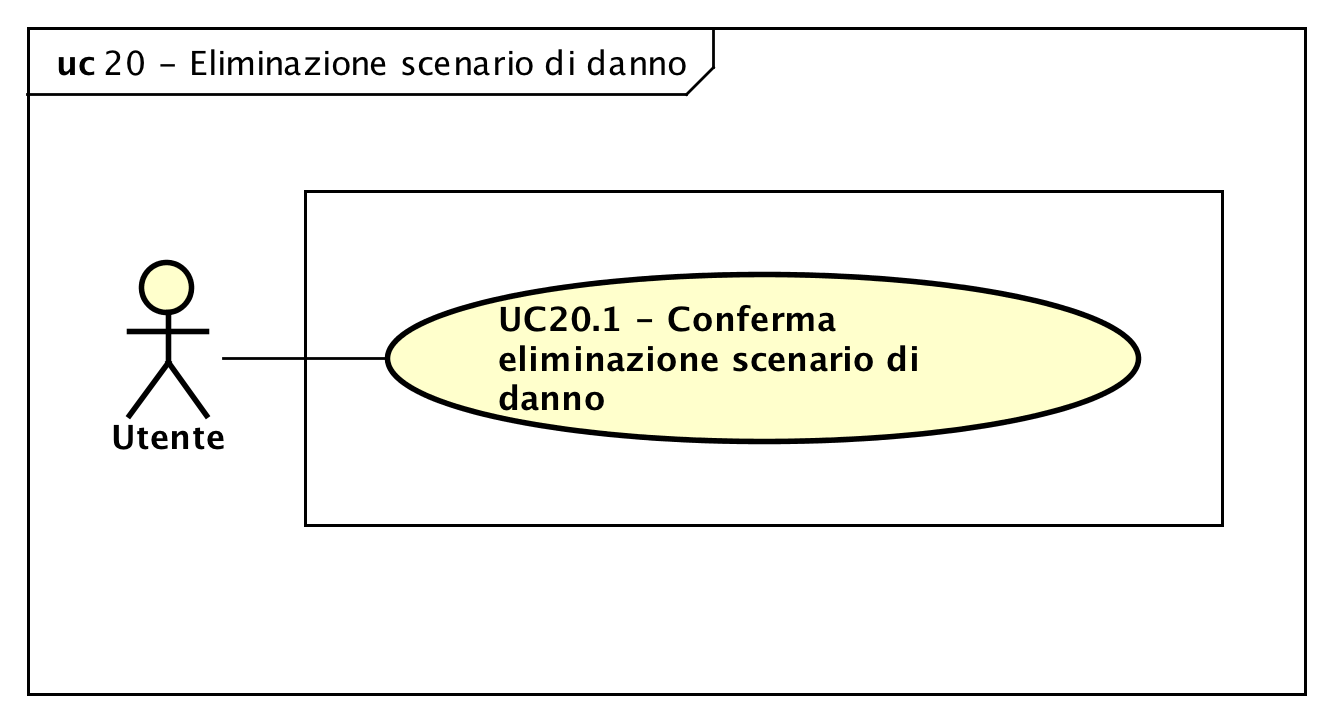
\includegraphics[scale=0.5]{{img/uc20}.png} 
	\caption{UC20 - Eliminazione scenario di danno}
\end{figure}
\def\arraystretch{1.5}
\rowcolors{2}{D}{P}
\begin{tabularx}{\textwidth}{l|p{0.7\textwidth}}
	\rowcolor{I} \multicolumn{2}{c}{\color{white}\textbf{UC20 - Eliminazione scenario di danno}} \\
	\toprule
	\endhead
	\textbf{Attori} & Utente\\
	\textbf{Descrizione} & l'utente elimina uno scenario\\
	\textbf{Pre-condizione} & l'utente ha aperto l'applicazione; è stato inserito almeno uno scenario; l'utente ha selezionato uno scenario\\
	\textbf{Post-condizione} & lo scenario è stato eliminato; l'utente visualizza un messaggio che comunica la corretta esecuzione dell'operazione;  l'area informativa viene impostata sulla visualizzazione di default;  la posizione e il livello di ingrandimento della mappa rimangono invariati\\
	\textbf{Scenario principale} & \vspace{-1.2em}\begin{enumerate}[leftmargin=*,noitemsep,nosep]
		\item \nameref{sssec:UC20.1}.
	\end{enumerate}\\
	\textbf{Estensioni} & \vspace{-1.2em}\begin{itemize}[leftmargin=*,noitemsep,nosep]
		\item \nameref{sssec:UC41}: l'utente interrompe volontariamente l'eliminazione dello
		scenario di danno
	\end{itemize}\\
	%\textbf{Generalizzazioni} &  \\
	\bottomrule
\end{tabularx}
\subsection{UC20.1 - Conferma eliminazione scenario di danno} 
\label{sssec:UC20.1} 
\def\arraystretch{1.5}
\rowcolors{2}{D}{P}
\begin{tabularx}{\textwidth}{l|p{0.7\textwidth}}
	\rowcolor{I} \multicolumn{2}{c}{\color{white}\textbf{UC20.1 - Conferma eliminazione scenario di danno}} \\
	\toprule
	\endhead
	\textbf{Attori} & Utente\\
	\textbf{Descrizione} & l'utente conferma l'eliminazione dello scenario di danno\\
	\textbf{Pre-condizione} & il sistema offre la possibilità di confermare l'eliminazione dello scenario di danno\\
	\textbf{Post-condizione} & lo scenario è stato eliminato; l'utente visualizza un messaggio che comunica la corretta esecuzione dell'operazione;  l'area informativa viene impostata sulla visualizzazione di default;  la posizione e il livello di ingrandimento della mappa rimangono invariati\\
		\textbf{Scenario principale} & \vspace{-1.2em}\begin{enumerate}[leftmargin=*,noitemsep,nosep]
		\item \nameref{sssec:UC20.1}.
	\end{enumerate}\\
	%\textbf{Generalizzazioni} &  \\
	\bottomrule
\end{tabularx}
\subsection{UC21 - Avvio analisi di danno} 
\label{sssec:UC21} 
\def\arraystretch{1.5}
\rowcolors{2}{D}{P}
\begin{tabularx}{\textwidth}{l|p{0.7\textwidth}}
	\rowcolor{I} \multicolumn{2}{c}{\color{white}\textbf{UC21 - Avvio analisi di danno}} \\
	\toprule
	\endhead
	\textbf{Attori} & Utente\\
	\textbf{Descrizione} & l'utente avvia l'analisi di danno\\
	\textbf{Pre-condizione} & l'utente ha aperto l'applicazione\\
	\textbf{Post-condizione} & la richiesta di processo dell'analisi di danno è stata inviata al server di calcolo; l'utente visualizza un messaggio riguardante l'invio della richiesta\\
	\textbf{Scenario principale} & \vspace{-1.2em}\begin{enumerate}[leftmargin=*,noitemsep,nosep]
		\item \nameref{sssec:UC21}.
	\end{enumerate}\\
	%\textbf{Generalizzazioni} &  \\
	\bottomrule
\end{tabularx}
\subsection{UC22 - Visualizzazione risultato analisi di danno su mappa} 
\label{sssec:UC22} 
\def\arraystretch{1.5}
\rowcolors{2}{D}{P}
\begin{tabularx}{\textwidth}{l|p{0.7\textwidth}}
	\rowcolor{I} \multicolumn{2}{c}{\color{white}\textbf{UC22 - Visualizzazione risultato analisi di danno su mappa}} \\
	\toprule
	\endhead
	\textbf{Attori} & Utente\\
	\textbf{Descrizione} & l'utente visualizza il risultato dell'analisi di danno sulla mappa\\
	\textbf{Pre-condizione} & l'utente ha aperto l'applicazione; i risultati dell'analisi di danno sono stati ricevuti\\
	\textbf{Post-condizione} & viene visualizzata su mappa il risultato dell'analisi di danno\\
	\textbf{Scenario principale} & \vspace{-1.2em}\begin{enumerate}[leftmargin=*,noitemsep,nosep]
		\item \nameref{sssec:UC22}.
	\end{enumerate}\\
	%\textbf{Generalizzazioni} &  \\
	\bottomrule
\end{tabularx}
\subsection{UC23 - Chiusura visualizzazione risultato analisi di danno su mappa} 
\label{sssec:UC23} 
\def\arraystretch{1.5}
\rowcolors{2}{D}{P}
\begin{tabularx}{\textwidth}{l|p{0.7\textwidth}}
	\rowcolor{I} \multicolumn{2}{c}{\color{white}\textbf{UC23 - Chiusura visualizzazione risultato analisi di danno su mappa}} \\
	\toprule
	\endhead
	\textbf{Attori} & Utente\\
	\textbf{Descrizione} & l'utente chiude la visualizzazione dell'analisi di danno sulla mappa\\
	\textbf{Pre-condizione} & l'utente ha aperto l'applicazione; i risultati dell'analisi di danno sono visualizzati\\
	\textbf{Post-condizione} & i risultati dell'analisi di danno non sono più visualizzati sulla mappa;  l'area informativa viene impostata sulla visualizzazione di default; la posizione e il livello di ingrandimento della mappa rimangono invariati\\
	\textbf{Scenario principale} & \vspace{-1.2em}\begin{enumerate}[leftmargin=*,noitemsep,nosep]
		\item \nameref{sssec:UC23}.
	\end{enumerate}\\
	%\textbf{Generalizzazioni} &  \\
	\bottomrule
\end{tabularx}
\subsection{UC24 - Interazione con la mappa} 
\label{sssec:UC24} 
\begin{figure}[H] 
	\centering 
	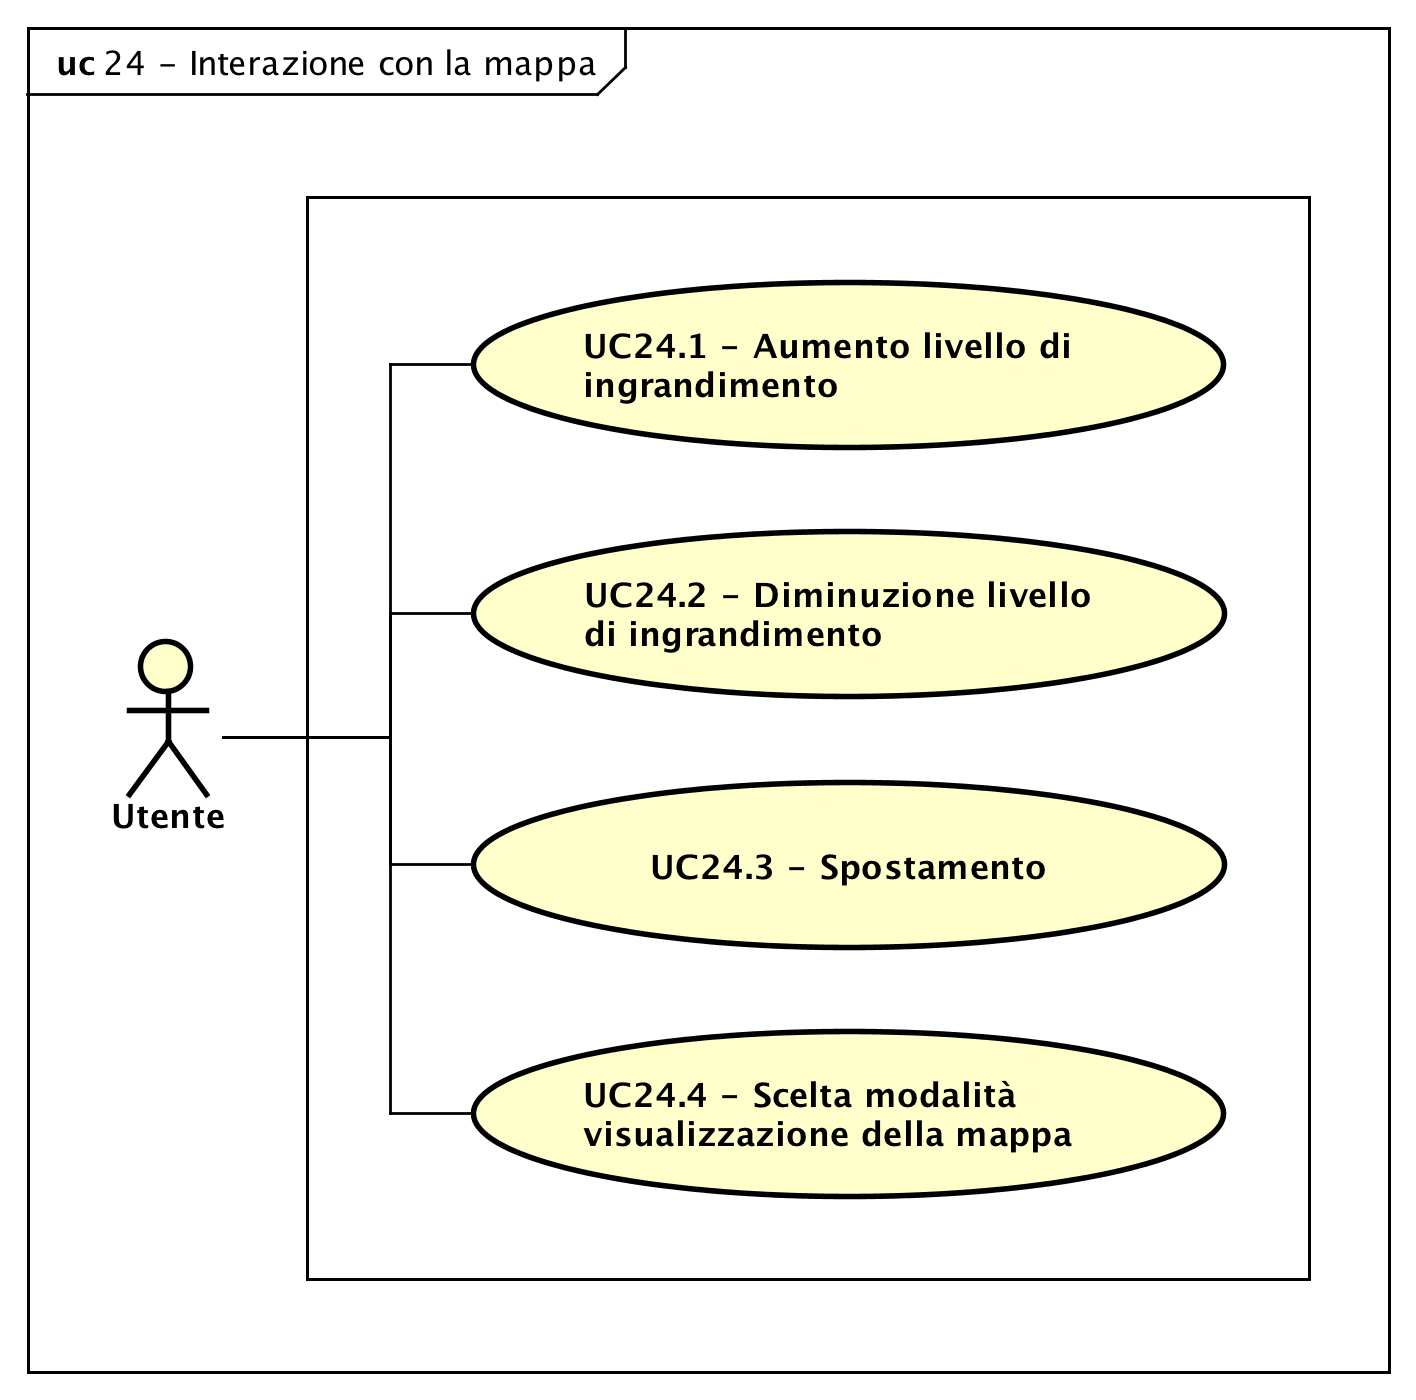
\includegraphics[scale=0.5]{{img/uc24}.png} 
	\caption{UC24 - Interazione con la mappa}
\end{figure}
\def\arraystretch{1.5}
\rowcolors{2}{D}{P}
\begin{tabularx}{\textwidth}{l|p{0.7\textwidth}}
	\rowcolor{I} \multicolumn{2}{c}{\color{white}\textbf{UC24 - Interazione con la mappa}} \\
	\toprule
	\endhead
	\textbf{Attori} & Utente\\
	\textbf{Descrizione} & l'utente interagisce con la mappa\\
	\textbf{Pre-condizione} & l'utente ha aperto l'applicazione\\
	\textbf{Post-condizione} & la mappa ha subito un'interazione; la visualizzazione della mappa è cambiata\\
	\textbf{Scenario principale} & \vspace{-1.2em}\begin{enumerate}[leftmargin=*,noitemsep,nosep]
		\item \nameref{sssec:UC24.1};
		\item \nameref{sssec:UC24.2};
		\item \nameref{sssec:UC24.3};
		\item \nameref{sssec:UC24.4}.
	\end{enumerate}\\
	%\textbf{Generalizzazioni} &  \\
	\bottomrule
\end{tabularx}
\subsection{UC24.1 - Aumento livello di ingrandimento} 
\label{sssec:UC24.1} 
\def\arraystretch{1.5}
\rowcolors{2}{D}{P}
\begin{tabularx}{\textwidth}{l|p{0.7\textwidth}}
	\rowcolor{I} \multicolumn{2}{c}{\color{white}\textbf{UC24.1 - Aumento livello di ingrandimento}} \\
	\toprule
	\endhead
	\textbf{Attori} & Utente\\
	\textbf{Descrizione} & l'utente aumenta il livello di ingrandimento della mappa\\
	\textbf{Pre-condizione} & l'utente ha aperto l'applicazione; il livello di zoom della mappa può essere aumentato\\
	\textbf{Post-condizione} & il livello di zoom della mappa è stato aumentato\\
	\textbf{Scenario principale} & \vspace{-1.2em}\begin{enumerate}[leftmargin=*,noitemsep,nosep]
		\item \nameref{sssec:UC24.1}.
	\end{enumerate}\\
	%\textbf{Generalizzazioni} &  \\
	\bottomrule
\end{tabularx}
\subsection{UC24.2 - Diminuzione livello di ingrandimento} 
\label{sssec:UC24.2} 
\def\arraystretch{1.5}
\rowcolors{2}{D}{P}
\begin{tabularx}{\textwidth}{l|p{0.7\textwidth}}
	\rowcolor{I} \multicolumn{2}{c}{\color{white}\textbf{UC24.2 - Diminuzione livello di ingrandimento}} \\
	\toprule
	\endhead
	\textbf{Attori} & Utente\\
	\textbf{Descrizione} & l'utente diminuisce il livello di ingrandimento della mappa\\
	\textbf{Pre-condizione} & l'utente ha aperto l'applicazione; il livello di zoom della mappa può essere diminuito\\
	\textbf{Post-condizione} & il livello di zoom della mappa è stato diminuito\\
	\textbf{Scenario principale} & \vspace{-1.2em}\begin{enumerate}[leftmargin=*,noitemsep,nosep]
		\item \nameref{sssec:UC24.2}.
	\end{enumerate}\\
	%\textbf{Generalizzazioni} &  \\
	\bottomrule
\end{tabularx}
\subsection{UC24.3 - Spostamento} 
\label{sssec:UC24.3} 
\def\arraystretch{1.5}
\rowcolors{2}{D}{P}
\begin{tabularx}{\textwidth}{l|p{0.7\textwidth}}
	\rowcolor{I} \multicolumn{2}{c}{\color{white}\textbf{UC24.3 - Spostamento}} \\
	\toprule
	\endhead
	\textbf{Attori} & Utente\\
	\textbf{Descrizione} & l'utente sposta la visualizzazione della mappa\\
	\textbf{Pre-condizione} & l'utente ha aperto l'applicazione; la visualizzazione della mappa può essere spostata\\
	\textbf{Post-condizione} & la visualizzazione della mappa è stata spostata\\
	\textbf{Scenario principale} & \vspace{-1.2em}\begin{enumerate}[leftmargin=*,noitemsep,nosep]
		\item \nameref{sssec:UC24.3}.
	\end{enumerate}\\
	%\textbf{Generalizzazioni} &  \\
	\bottomrule
\end{tabularx}
\subsection{UC24.4 - Scelta modalità visualizzazione della mappa} 
\label{sssec:UC24.4} 
\def\arraystretch{1.5}
\rowcolors{2}{D}{P}
\begin{tabularx}{\textwidth}{l|p{0.7\textwidth}}
	\rowcolor{I} \multicolumn{2}{c}{\color{white}\textbf{UC24.4 - Scelta modalità visualizzazione della mappa}} \\
	\toprule
	\endhead
	\textbf{Attori} & Utente\\
	\textbf{Descrizione} & l'utente sceglie la modalità di visualizzazione della mappa\\
	\textbf{Pre-condizione} & l'utente ha aperto l'applicazione; la modalità di visualizzazione della mappa può essere scelta\\
	\textbf{Post-condizione} & la modalità di visualizzazione della mappa è stata scelta; la mappa cambia di conseguenza\\
	\textbf{Scenario principale} & \vspace{-1.2em}\begin{enumerate}[leftmargin=*,noitemsep,nosep]
		\item \nameref{sssec:UC24.4}.
	\end{enumerate}\\
	%\textbf{Generalizzazioni} &  \\
	\bottomrule
\end{tabularx}
\subsection{UC25 - Fruizione tutorial} 
\label{sssec:UC25} 
\def\arraystretch{1.5}
\rowcolors{2}{D}{P}
\begin{tabularx}{\textwidth}{l|p{0.7\textwidth}}
	\rowcolor{I} \multicolumn{2}{c}{\color{white}\textbf{UC25 - Avvio tutorial}} \\
	\toprule
	\endhead
	\textbf{Attori} & Utente\\
	\textbf{Descrizione} & l'utente avvia il tutorial ed esegue tutte le operazioni che l'applicazione offre in modo guidato\\
	\textbf{Pre-condizione} & l'utente ha aperto l'applicazione; il tutorial può essere avviato\\
	\textbf{Post-condizione} & il tutorial è stato completato; l'area informativa viene impostata alla visualizzazione di default; durante l'esecuzione del tutorial vengono visualizzate informazioni relative alle varie operazioni che l'utente può eseguire; l'utente può eseguire tutte le operazioni permesse dal sistema in modo guidato\\
	\textbf{Scenario principale} & \vspace{-1.2em}\begin{enumerate}[leftmargin=*,noitemsep,nosep]
		\item \nameref{sssec:UC25}.
	\end{enumerate}\\
	\textbf{Estensioni} & \vspace{-1.2em}\begin{itemize}[leftmargin=*,noitemsep,nosep]
	\item \nameref{sssec:UC46}: l'utente interrompe volontariamente
	la fruizione del tutorial
\end{itemize}\\
	%\textbf{Generalizzazioni} &  \\
	\bottomrule
\end{tabularx}
\subsection{UC26 - Fruizione assistente vocale} 
\label{sssec:UC26} 
\def\arraystretch{1.5}
\rowcolors{2}{D}{P}
\begin{tabularx}{\textwidth}{l|p{0.7\textwidth}}
	\rowcolor{I} \multicolumn{2}{c}{\color{white}\textbf{UC26 - Avvio assistente vocale}} \\
	\toprule
	\endhead
	\textbf{Attori} & Utente\\
	\textbf{Descrizione} & l'utente avvia l'assistente vocale ed esegue le operazioni con l'ausilio della voce\\
	\textbf{Pre-condizione} & l'utente ha aperto l'applicazione; l'assistente vocale può essere avviato\\
	\textbf{Post-condizione} & l'assistente vocale ha effettuato l'operazione chiesta dall'utente; l'area informativa viene impostata alla visualizzazione di default; durante l'esecuzione dell'assistente vocale l'utente può eseguire tutte le operazioni permesse dal sistema con l'ausilio della voce\\
	\textbf{Scenario principale} & \vspace{-1.2em}\begin{enumerate}[leftmargin=*,noitemsep,nosep]
		\item \nameref{sssec:UC26}.
	\end{enumerate}\\
	%\textbf{Generalizzazioni} &  \\
	\bottomrule
\end{tabularx}
\subsection{UC27 - Ritorno visuale asset selezionato} 
\label{sssec:UC27} 
\def\arraystretch{1.5}
\rowcolors{2}{D}{P}
\begin{tabularx}{\textwidth}{l|p{0.7\textwidth}}
	\rowcolor{I} \multicolumn{2}{c}{\color{white}\textbf{UC27 - Ritorno visuale asset selezionato}} \\
	\toprule
	\endhead
	\textbf{Attori} & Utente\\
	\textbf{Descrizione} & l'utente viene riportato alla visualizzazione dell'asset selezionato\\
	\textbf{Pre-condizione} & l'utente ha visualizzato le informazioni di un asset\\
	\textbf{Post-condizione} & il sistema riporta la visualizzazione della mappa in modo tale da visualizzare i nodi all'interno dell'asset selezionato\\
	\textbf{Scenario principale} & \vspace{-1.2em}\begin{enumerate}[leftmargin=*,noitemsep,nosep]
		\item \nameref{sssec:UC27}.
	\end{enumerate}\\
	%\textbf{Generalizzazioni} &  \\
	\bottomrule
\end{tabularx}
\subsection{UC28 - Ritorno visuale nodo selezionato} 
\label{sssec:UC28} 
\def\arraystretch{1.5}
\rowcolors{2}{D}{P}
\begin{tabularx}{\textwidth}{l|p{0.7\textwidth}}
	\rowcolor{I} \multicolumn{2}{c}{\color{white}\textbf{UC28 - Ritorno visuale nodo selezionato}} \\
	\toprule
	\endhead
	\textbf{Attori} & Utente\\
	\textbf{Descrizione} & l'utente viene riportato alla visualizzazione del nodo selezionato\\
	\textbf{Pre-condizione} & l'utente ha visualizzato le informazioni di un nodo\\
	\textbf{Post-condizione} & il sistema riporta la visualizzazione della mappa in modo tale da visualizzare il nodo selezionato\\
	\textbf{Scenario principale} & \vspace{-1.2em}\begin{enumerate}[leftmargin=*,noitemsep,nosep]
		\item \nameref{sssec:UC28}.
	\end{enumerate}\\
	%\textbf{Generalizzazioni} &  \\
	\bottomrule
\end{tabularx}
\subsection{UC29 - Ritorno visuale arco selezionato} 
\label{sssec:UC29} 
\def\arraystretch{1.5}
\rowcolors{2}{D}{P}
\begin{tabularx}{\textwidth}{l|p{0.7\textwidth}}
	\rowcolor{I} \multicolumn{2}{c}{\color{white}\textbf{UC29 - Ritorno visuale arco selezionato}} \\
	\toprule
	\endhead
	\textbf{Attori} & Utente\\
	\textbf{Descrizione} & l'utente viene riportato alla visualizzazione dell'arco selezionato\\
	\textbf{Pre-condizione} & l'utente ha visualizzato le informazioni di un arco\\
	\textbf{Post-condizione} & il sistema riporta la visualizzazione della mappa in modo tale da visualizzare l'arco selezionato\\
	\textbf{Scenario principale} & \vspace{-1.2em}\begin{enumerate}[leftmargin=*,noitemsep,nosep]
		\item \nameref{sssec:UC29}.
	\end{enumerate}\\
	%\textbf{Generalizzazioni} &  \\
	\bottomrule
\end{tabularx}

\subsection{UC30 - Interruzione aggiunta asset} 
\label{sssec:UC30} 
\def\arraystretch{1.5}
\rowcolors{2}{D}{P}
\begin{tabularx}{\textwidth}{l|p{0.7\textwidth}}
	\rowcolor{I} \multicolumn{2}{c}{\color{white}\textbf{UC30 - Interruzione aggiunta asset}} \\
	\toprule
	\endhead
	\textbf{Attori} & Utente\\
	\textbf{Descrizione} & l'utente interrompe l'aggiunta dell'asset\\
	\textbf{Pre-condizione} & il sistema offre la possibilità di aggiungere un asset\\
	\textbf{Post-condizione} & nessun asset è stato aggiunto; l'area informativa viene impostata sulla visualizzazione di default; la posizione e il livello di ingrandimento della mappa rimangono invariati\\
	\textbf{Scenario principale} & \vspace{-1.2em}\begin{enumerate}[leftmargin=*,noitemsep,nosep]
		\item \nameref{sssec:UC30}.
	\end{enumerate}\\
	%\textbf{Generalizzazioni} &  \\
	\bottomrule
\end{tabularx}
\subsection{UC31 - Interruzione modifica asset} 
\label{sssec:UC31} 
\def\arraystretch{1.5}
\rowcolors{2}{D}{P}
\begin{tabularx}{\textwidth}{l|p{0.7\textwidth}}
	\rowcolor{I} \multicolumn{2}{c}{\color{white}\textbf{UC31 - Interruzione modifica asset}} \\
	\toprule
	\endhead
	\textbf{Attori} & Utente\\
	\textbf{Descrizione} & l'utente interrompe la modifica dell'asset\\
	\textbf{Pre-condizione} & il sistema offre la possibilità di modificare un asset\\
	\textbf{Post-condizione} & l'asset non è stato modificato; l'area informativa viene impostata sulla visualizzazione di default; la posizione e il livello di ingrandimento della mappa rimangono invariati\\
	\textbf{Scenario principale} & \vspace{-1.2em}\begin{enumerate}[leftmargin=*,noitemsep,nosep]
		\item \nameref{sssec:UC31}.
	\end{enumerate}\\
	%\textbf{Generalizzazioni} &  \\
	\bottomrule
\end{tabularx}
\subsection{UC32 - Interruzione eliminazione asset} 
\label{sssec:UC32} 
\def\arraystretch{1.5}
\rowcolors{2}{D}{P}
\begin{tabularx}{\textwidth}{l|p{0.7\textwidth}}
	\rowcolor{I} \multicolumn{2}{c}{\color{white}\textbf{UC32 - Interruzione eliminazione asset}} \\
	\toprule
	\endhead
	\textbf{Attori} & Utente\\
	\textbf{Descrizione} & l'utente interrompe l'eliminazione dell'asset\\
	\textbf{Pre-condizione} & il sistema offre la possibilità di confermare l'eliminazione dell'asset\\
	\textbf{Post-condizione} & l'asset non è stato eliminato; l'area informativa viene impostata sulla visualizzazione di default; la posizione e il livello di ingrandimento della mappa rimangono invariati\\
	\textbf{Scenario principale} & \vspace{-1.2em}\begin{enumerate}[leftmargin=*,noitemsep,nosep]
		\item \nameref{sssec:UC32}.
	\end{enumerate}\\
	%\textbf{Generalizzazioni} &  \\
	\bottomrule
\end{tabularx}
\subsection{UC33 - Interruzione aggiunta nodo} 
\label{sssec:UC33} 
\def\arraystretch{1.5}
\rowcolors{2}{D}{P}
\begin{tabularx}{\textwidth}{l|p{0.7\textwidth}}
	\rowcolor{I} \multicolumn{2}{c}{\color{white}\textbf{UC33 - Interruzione aggiunta nodo}} \\
	\toprule
	\endhead
	\textbf{Attori} & Utente\\
	\textbf{Descrizione} & l'utente interrompe l'aggiunta di un nodo\\
	\textbf{Pre-condizione} & il sistema offre la possibilità di aggiungere un nodo\\
	\textbf{Post-condizione} & nessun nuovo nodo è stato aggiunto;  l'area informativa viene impostata sulla visualizzazione di default; la posizione e il livello di ingrandimento della mappa rimangono invariati\\
	\textbf{Scenario principale} & \vspace{-1.2em}\begin{enumerate}[leftmargin=*,noitemsep,nosep]
		\item \nameref{sssec:UC33}.
	\end{enumerate}\\
	%\textbf{Generalizzazioni} &  \\
	\bottomrule
\end{tabularx}
\subsection{UC34 - Interruzione modifica nodo} 
\label{sssec:UC34} 
\def\arraystretch{1.5}
\rowcolors{2}{D}{P}
\begin{tabularx}{\textwidth}{l|p{0.7\textwidth}}
	\rowcolor{I} \multicolumn{2}{c}{\color{white}\textbf{UC34 - Interruzione modifica nodo}} \\
	\toprule
	\endhead
	\textbf{Attori} & Utente\\
	\textbf{Descrizione} & l'utente interrompe la modifica del nodo\\
	\textbf{Pre-condizione} & il sistema offre la possibilità di modificare un nodo\\
	\textbf{Post-condizione} & il nodo non è stato modificato;  l'area informativa viene impostata sulla visualizzazione di default; la posizione e il livello di ingrandimento della mappa rimangono invariati\\
	\textbf{Scenario principale} & \vspace{-1.2em}\begin{enumerate}[leftmargin=*,noitemsep,nosep]
		\item \nameref{sssec:UC34}.
	\end{enumerate}\\
	%\textbf{Generalizzazioni} &  \\
	\bottomrule
\end{tabularx}
\subsection{UC35 - Interruzione eliminazione nodo} 
\label{sssec:UC35} 
\def\arraystretch{1.5}
\rowcolors{2}{D}{P}
\begin{tabularx}{\textwidth}{l|p{0.7\textwidth}}
	\rowcolor{I} \multicolumn{2}{c}{\color{white}\textbf{UC35 - Interruzione eliminazione nodo}} \\
	\toprule
	\endhead
	\textbf{Attori} & Utente\\
	\textbf{Descrizione} & l'utente interrompe l'eliminazione del nodo\\
	\textbf{Pre-condizione} & il sistema offre la possibilità di confermare l'eliminazione del nodo\\
	\textbf{Post-condizione} & il nodo non è stato eliminato e rimane visibile sulla mappa; l'area informativa viene impostata sulla visualizzazione di default;  la posizione e il livello di ingrandimento della mappa rimangono invariati\\
	\textbf{Scenario principale} & \vspace{-1.2em}\begin{enumerate}[leftmargin=*,noitemsep,nosep]
		\item \nameref{sssec:UC35}.
	\end{enumerate}\\
	%\textbf{Generalizzazioni} &  \\
	\bottomrule
\end{tabularx}
\subsection{UC36 - Interruzione aggiunta arco} 
\label{sssec:UC36} 
\def\arraystretch{1.5}
\rowcolors{2}{D}{P}
\begin{tabularx}{\textwidth}{l|p{0.7\textwidth}}
	\rowcolor{I} \multicolumn{2}{c}{\color{white}\textbf{UC36 - Interruzione aggiunta arco}} \\
	\toprule
	\endhead
	\textbf{Attori} & Utente\\
	\textbf{Descrizione} & l'utente interrompe l'aggiunta dell'arco\\
	\textbf{Pre-condizione} & il sistema offre la possibilità di aggiungere un arco\\
	\textbf{Post-condizione} & nessun arco è stato aggiunto; l'area informativa viene impostata sulla visualizzazione di default; la posizione e il livello di ingrandimento della mappa rimangono invariati\\
	\textbf{Scenario principale} & \vspace{-1.2em}\begin{enumerate}[leftmargin=*,noitemsep,nosep]
		\item \nameref{sssec:UC36}.
	\end{enumerate}\\
	%\textbf{Generalizzazioni} &  \\
	\bottomrule
\end{tabularx}
\subsection{UC37 - Interruzione modifica arco} 
\label{sssec:UC37} 
\def\arraystretch{1.5}
\rowcolors{2}{D}{P}
\begin{tabularx}{\textwidth}{l|p{0.7\textwidth}}
	\rowcolor{I} \multicolumn{2}{c}{\color{white}\textbf{UC37 - Interruzione modifica arco}} \\
	\toprule
	\endhead
	\textbf{Attori} & Utente\\
	\textbf{Descrizione} & l'utente interrompe la modifica dell'arco\\
	\textbf{Pre-condizione} & il sistema offre la possibilità di modificare un arco\\
	\textbf{Post-condizione} & l'arco non è stato modificato; l'area informativa viene impostata sulla visualizzazione di default; la posizione e il livello di ingrandimento della mappa rimangono invariati\\
	\textbf{Scenario principale} & \vspace{-1.2em}\begin{enumerate}[leftmargin=*,noitemsep,nosep]
		\item \nameref{sssec:UC37}.
	\end{enumerate}\\
	%\textbf{Generalizzazioni} &  \\
	\bottomrule
\end{tabularx}
\subsection{UC38 - Interruzione eliminazione arco} 
\label{sssec:UC38} 
\def\arraystretch{1.5}
\rowcolors{2}{D}{P}
\begin{tabularx}{\textwidth}{l|p{0.7\textwidth}}
	\rowcolor{I} \multicolumn{2}{c}{\color{white}\textbf{UC38 - Interruzione eliminazione arco}} \\
	\toprule
	\endhead
	\textbf{Attori} & Utente\\
	\textbf{Descrizione} & l'utente interrompe l'eliminazione dell'arco\\
	\textbf{Pre-condizione} & il sistema offre la possibilità di confermare l'eliminazione dell'arco\\
	\textbf{Post-condizione} & l'arco non è stato eliminato ed è ancora visibile sulla mappa; l'area informativa viene impostata sulla visualizzazione di default;  la posizione e il livello di ingrandimento della mappa rimangono invariati\\
	\textbf{Scenario principale} & \vspace{-1.2em}\begin{enumerate}[leftmargin=*,noitemsep,nosep]
		\item \nameref{sssec:UC38}.
	\end{enumerate}\\
	%\textbf{Generalizzazioni} &  \\
	\bottomrule
\end{tabularx}
\subsection{UC39 - Interruzione aggiunta scenario di danno} 
\label{sssec:UC39} 
\def\arraystretch{1.5}
\rowcolors{2}{D}{P}
\begin{tabularx}{\textwidth}{l|p{0.7\textwidth}}
	\rowcolor{I} \multicolumn{2}{c}{\color{white}\textbf{UC39 - Interruzione aggiunta scenario di danno}} \\
	\toprule
	\endhead
	\textbf{Attori} & Utente\\
	\textbf{Descrizione} & l'utente interrompe l'aggiunta dello scenario di danno\\
	\textbf{Pre-condizione} & il sistema offre la possibilità di aggiungere uno scenario di danno\\
	\textbf{Post-condizione} & nessuno scenario è stato aggiunto; l'area informativa viene impostata sulla visualizzazione di default; la posizione e il livello di ingrandimento della mappa rimangono invariati\\
	\textbf{Scenario principale} & \vspace{-1.2em}\begin{enumerate}[leftmargin=*,noitemsep,nosep]
		\item \nameref{sssec:UC39}: l’utente interrompe volontariamente l’aggiunta dello
		scenario di danno;
	\end{enumerate}\\
	%\textbf{Generalizzazioni} &  \\
	\bottomrule
\end{tabularx}

\subsection{UC40 - Interruzione modifica scenario} 
\label{sssec:UC40} 
\def\arraystretch{1.5}
\rowcolors{2}{D}{P}
\begin{tabularx}{\textwidth}{l|p{0.7\textwidth}}
	\rowcolor{I} \multicolumn{2}{c}{\color{white}\textbf{UC40 - Interruzione modifica scenario}} \\
	\toprule
	\endhead
	\textbf{Attori} & Utente\\
	\textbf{Descrizione} & l'utente interrompe la modifica dello scenario\\
	\textbf{Pre-condizione} & il sistema offre la possibilità di modificare lo scenario\\
	\textbf{Post-condizione} & lo scenario non è stato modificato;  l'area informativa viene impostata sulla visualizzazione di default; la posizione e il livello di ingrandimento della mappa rimangono invariati\\
	\textbf{Scenario principale} & \vspace{-1.2em}\begin{enumerate}[leftmargin=*,noitemsep,nosep]
		\item \nameref{sssec:UC40}.
	\end{enumerate}\\
	%\textbf{Generalizzazioni} &  \\
	\bottomrule
\end{tabularx}
\subsection{UC41 - Interruzione eliminazione scenario di danno} 
\label{sssec:UC41} 
\def\arraystretch{1.5}
\rowcolors{2}{D}{P}
\begin{tabularx}{\textwidth}{l|p{0.7\textwidth}}
	\rowcolor{I} \multicolumn{2}{c}{\color{white}\textbf{UC41 - Interruzione eliminazione scenario di danno}} \\
	\toprule
	\endhead
	\textbf{Attori} & Utente\\
	\textbf{Descrizione} & l'utente interrompe l'eliminazione dello scenario di danno\\
	\textbf{Pre-condizione} & il sistema offre la possibilità di confermare l'eliminazione dello scenario di danno\\
	\textbf{Post-condizione} & lo scenario di danno non è stato eliminato;  l'area informativa viene impostata sulla visualizzazione di default;  la posizione e il livello di ingrandimento della mappa rimangono invariati
	\\
	\textbf{Scenario principale} & \vspace{-1.2em}\begin{enumerate}[leftmargin=*,noitemsep,nosep]
		\item \nameref{sssec:UC41}.
	\end{enumerate}\\
	%\textbf{Generalizzazioni} &  \\
	\bottomrule
\end{tabularx}
\subsection{UC42 - Selezione scenario di danno per analisi di danno} 
\label{sssec:UC42} 
\def\arraystretch{1.5}
\rowcolors{2}{D}{P}
\begin{tabularx}{\textwidth}{l|p{0.7\textwidth}}
	\rowcolor{I} \multicolumn{2}{c}{\color{white}\textbf{UC42 - Selezione scenario di danno per analisi di danno}} \\
	\toprule
	\endhead
	\textbf{Attori} & Utente\\
	\textbf{Descrizione} & l'utente aggiunge uno scenario di danno alla lista di quelli da prendere in considerazione per la successiva analisi\\
	\textbf{Pre-condizione} & è stato inserito almeno uno scenario di danno\\
	\textbf{Post-condizione} & lo scenario di dannno è stato aggiunto alla lista di quelli da prendere in considerazione per la successiva analisi; l'utente visualizza che lo scenario è stato selezionato \\
	\textbf{Scenario principale} & \vspace{-1.2em}\begin{enumerate}[leftmargin=*,noitemsep,nosep]
		\item \nameref{sssec:UC42}.
	\end{enumerate}\\
	%\textbf{Generalizzazioni} &  \\
	\bottomrule
\end{tabularx}
\subsection{UC43 - Deselezione scenario di danno per analisi di danno} 
\label{sssec:UC43} 
\def\arraystretch{1.5}
\rowcolors{2}{D}{P}
\begin{tabularx}{\textwidth}{l|p{0.7\textwidth}}
	\rowcolor{I} \multicolumn{2}{c}{\color{white}\textbf{UC43 - Deselezione scenario di danno per analisi di danno}} \\
	\toprule
	\endhead
	\textbf{Attori} & Utente\\
	\textbf{Descrizione} & l'utente rimuove uno scenario di danno dalla lista di quelli da prendere in considerazione per la successiva analisi\\
	\textbf{Pre-condizione} & è stato inserito almeno uno scenario di danno; è stato selezionato almeno uno scenario di danno per l'analisi di danno\\
	\textbf{Post-condizione} & lo scenario di dannno è stato rimosso alla lista di quelli da prendere in considerazione per la successiva analisi; l'utente visualizza che lo scenario è stato deselezionato \\
	\textbf{Scenario principale} & \vspace{-1.2em}\begin{enumerate}[leftmargin=*,noitemsep,nosep]
		\item \nameref{sssec:UC43}.
	\end{enumerate}\\
	%\textbf{Generalizzazioni} &  \\
	\bottomrule
\end{tabularx}
\subsection{UC44 - Eliminazione analisi di danno} 
\label{sssec:UC44} 
\begin{figure}[H] 
	\centering 
	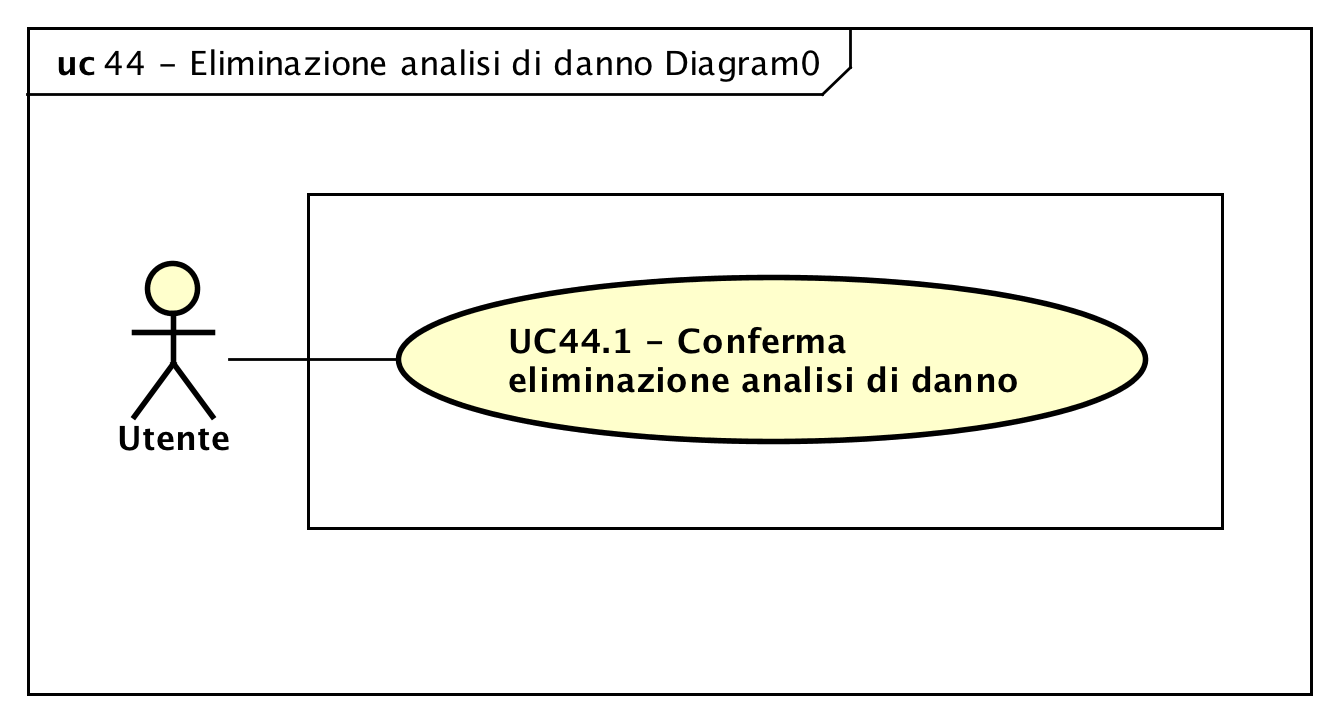
\includegraphics[scale=0.5]{{img/uc44}.png} 
	\caption{UC44 - Eliminazione analisi di danno}
\end{figure}
\def\arraystretch{1.5}
\rowcolors{2}{D}{P}
\begin{tabularx}{\textwidth}{l|p{0.7\textwidth}}
	\rowcolor{I} \multicolumn{2}{c}{\color{white}\textbf{UC44 - Eliminazione analisi di danno}} \\
	\toprule
	\endhead
	\textbf{Attori} & Utente\\
	\textbf{Descrizione} & l'utente elimina un analisi di danno precedentemente eseguita\\
	\textbf{Pre-condizione} & è stata calcolata almeno un'analisi di danno; è stata selezionata un'analisi di danno\\
	\textbf{Post-condizione} & l'analisi di danno è stata eliminata; l'utente visualizza un messaggio che comunica la corretta esecuzione dell'operazione;  l'area informativa viene impostata sulla visualizzazione di default;  la posizione e il livello di ingrandimento della mappa rimangono invariati\\
	\textbf{Estensioni} & \vspace{-1.2em}\begin{itemize}[leftmargin=*,noitemsep,nosep]
		\item \nameref{sssec:UC45}: l'utente interrompe volontariamente
		l'eliminazione dell'analisi di danno
	\end{itemize}\\
	%\textbf{Generalizzazioni} &  \\
	\bottomrule
\end{tabularx}
\subsection{UC44.1 - Conferma eliminazione analisi di danno} 
\label{sssec:UC44.1} 
\def\arraystretch{1.5}
\rowcolors{2}{D}{P}
\begin{tabularx}{\textwidth}{l|p{0.7\textwidth}}
	\rowcolor{I} \multicolumn{2}{c}{\color{white}\textbf{UC44.1 - Conferma eliminazione analisi di danno}} \\
	\toprule
	\endhead
	\textbf{Attori} & Utente\\
	\textbf{Descrizione} & l'utente conferma l'eliminazione dell'analisi di danno\\
	\textbf{Pre-condizione} & il sistema offre la possibilità di confermare l'eliminazione dell'analisi di danno\\
	\textbf{Post-condizione} & l'analisi di danno è stata eliminata; l'utente visualizza un messaggio che comunica la corretta esecuzione dell'operazione;  l'area informativa viene impostata sulla visualizzazione di default;  la posizione e il livello di ingrandimento della mappa rimangono invariati\\
	\textbf{Scenario principale} & \vspace{-1.2em}\begin{enumerate}[leftmargin=*,noitemsep,nosep]
		\item \nameref{sssec:UC44.1}.
	\end{enumerate}\\
	%\textbf{Generalizzazioni} &  \\
	\bottomrule
\end{tabularx}
\subsection{UC45 - Interruzione eliminazione analisi di danno} 
\label{sssec:UC45} 
\def\arraystretch{1.5}
\rowcolors{2}{D}{P}
\begin{tabularx}{\textwidth}{l|p{0.7\textwidth}}
	\rowcolor{I} \multicolumn{2}{c}{\color{white}\textbf{UC45 - Interruzione eliminazione analisi di danno}} \\
	\toprule
	\endhead
	\textbf{Attori} & Utente\\
	\textbf{Descrizione} & l'utente interrompe l'eliminazione dell'analisi di danno\\
	\textbf{Pre-condizione} & il sistema offre la possibilità di confermare l'eliminazione dell'analisi di danno\\
	\textbf{Post-condizione} & l'analisi di danno non è stata eliminata; l'area informativa viene impostata sulla visualizzazione di default; la posizione e il livello di ingrandimento della mappa rimangono invariati\\
	\textbf{Scenario principale} & \vspace{-1.2em}\begin{enumerate}[leftmargin=*,noitemsep,nosep]
		\item \nameref{sssec:UC45}.
	\end{enumerate}\\
	%\textbf{Generalizzazioni} &  \\
	\bottomrule
\end{tabularx}

\subsection{UC46 - Interruzione fruizione tutorial} 
\label{sssec:UC46} 
\def\arraystretch{1.5}
\rowcolors{2}{D}{P}
\begin{tabularx}{\textwidth}{l|p{0.7\textwidth}}
	\rowcolor{I} \multicolumn{2}{c}{\color{white}\textbf{UC46 - Interruzione fruizione tutorial}} \\
	\toprule
	\endhead
	\textbf{Attori} & Utente\\
	\textbf{Descrizione} & L'utente interrompe la fruizione del tutorial\\
	\textbf{Pre-condizione} & il tutorial sta eseguendo\\
	\textbf{Post-condizione} & l'utente ha interrotto la fruizione del tutorial; gli effetti delle operazioni eseguite all'interno del tutorial non vengono annullati; l'area informativa viene impostata alla visualizzazione di default\\
	\textbf{Scenario principale} & \vspace{-1.2em}\begin{enumerate}[leftmargin=*,noitemsep,nosep]
		\item \nameref{sssec:UC46}.
	\end{enumerate}\\
	%\textbf{Generalizzazioni} &  \\
	\bottomrule
\end{tabularx}
\subsection{UC47 - Interruzione fruizione assistente vocale} 
\label{sssec:UC47} 
\def\arraystretch{1.5}
\rowcolors{2}{D}{P}
\begin{tabularx}{\textwidth}{l|p{0.7\textwidth}}
	\rowcolor{I} \multicolumn{2}{c}{\color{white}\textbf{UC47 - Interruzione fruizione assistente vocale}} \\
	\toprule
	\endhead
	\textbf{Attori} & Utente\\
	\textbf{Descrizione} & L'utente interrompe la fruizione dell'assistente vocale\\
	\textbf{Pre-condizione} & l'assistente vocale sta eseguendo\\
	\textbf{Post-condizione} & l'utente ha interrotto la fruizione del tutorial; nessuna operazione è stata eseguita dall'assistente vocale; l'area informativa viene impostata alla visualizzazione di default\\
	\textbf{Scenario principale} & \vspace{-1.2em}\begin{enumerate}[leftmargin=*,noitemsep,nosep]
		\item \nameref{sssec:UC47}.
	\end{enumerate}\\
	%\textbf{Generalizzazioni} &  \\
	\bottomrule
\end{tabularx}
